% Options for packages loaded elsewhere
% Options for packages loaded elsewhere
\PassOptionsToPackage{unicode}{hyperref}
\PassOptionsToPackage{hyphens}{url}
%
\documentclass[
  letterpaper,
]{scrbook}
\usepackage{xcolor}
\usepackage{amsmath,amssymb}
\setcounter{secnumdepth}{5}
\usepackage{iftex}
\ifPDFTeX
  \usepackage[T1]{fontenc}
  \usepackage[utf8]{inputenc}
  \usepackage{textcomp} % provide euro and other symbols
\else % if luatex or xetex
  \usepackage{unicode-math} % this also loads fontspec
  \defaultfontfeatures{Scale=MatchLowercase}
  \defaultfontfeatures[\rmfamily]{Ligatures=TeX,Scale=1}
\fi
\usepackage{lmodern}
\ifPDFTeX\else
  % xetex/luatex font selection
\fi
% Use upquote if available, for straight quotes in verbatim environments
\IfFileExists{upquote.sty}{\usepackage{upquote}}{}
\IfFileExists{microtype.sty}{% use microtype if available
  \usepackage[]{microtype}
  \UseMicrotypeSet[protrusion]{basicmath} % disable protrusion for tt fonts
}{}
\makeatletter
\@ifundefined{KOMAClassName}{% if non-KOMA class
  \IfFileExists{parskip.sty}{%
    \usepackage{parskip}
  }{% else
    \setlength{\parindent}{0pt}
    \setlength{\parskip}{6pt plus 2pt minus 1pt}}
}{% if KOMA class
  \KOMAoptions{parskip=half}}
\makeatother
% Make \paragraph and \subparagraph free-standing
\makeatletter
\ifx\paragraph\undefined\else
  \let\oldparagraph\paragraph
  \renewcommand{\paragraph}{
    \@ifstar
      \xxxParagraphStar
      \xxxParagraphNoStar
  }
  \newcommand{\xxxParagraphStar}[1]{\oldparagraph*{#1}\mbox{}}
  \newcommand{\xxxParagraphNoStar}[1]{\oldparagraph{#1}\mbox{}}
\fi
\ifx\subparagraph\undefined\else
  \let\oldsubparagraph\subparagraph
  \renewcommand{\subparagraph}{
    \@ifstar
      \xxxSubParagraphStar
      \xxxSubParagraphNoStar
  }
  \newcommand{\xxxSubParagraphStar}[1]{\oldsubparagraph*{#1}\mbox{}}
  \newcommand{\xxxSubParagraphNoStar}[1]{\oldsubparagraph{#1}\mbox{}}
\fi
\makeatother


\usepackage{longtable,booktabs,array}
\newcounter{none} % for unnumbered tables
\usepackage{calc} % for calculating minipage widths
% Correct order of tables after \paragraph or \subparagraph
\usepackage{etoolbox}
\makeatletter
\patchcmd\longtable{\par}{\if@noskipsec\mbox{}\fi\par}{}{}
\makeatother
% Allow footnotes in longtable head/foot
\IfFileExists{footnotehyper.sty}{\usepackage{footnotehyper}}{\usepackage{footnote}}
\makesavenoteenv{longtable}
\usepackage{graphicx}
\makeatletter
\newsavebox\pandoc@box
\newcommand*\pandocbounded[1]{% scales image to fit in text height/width
  \sbox\pandoc@box{#1}%
  \Gscale@div\@tempa{\textheight}{\dimexpr\ht\pandoc@box+\dp\pandoc@box\relax}%
  \Gscale@div\@tempb{\linewidth}{\wd\pandoc@box}%
  \ifdim\@tempb\p@<\@tempa\p@\let\@tempa\@tempb\fi% select the smaller of both
  \ifdim\@tempa\p@<\p@\scalebox{\@tempa}{\usebox\pandoc@box}%
  \else\usebox{\pandoc@box}%
  \fi%
}
% Set default figure placement to htbp
\def\fps@figure{htbp}
\makeatother


% definitions for citeproc citations
\NewDocumentCommand\citeproctext{}{}
\NewDocumentCommand\citeproc{mm}{%
  \begingroup\def\citeproctext{#2}\cite{#1}\endgroup}
\makeatletter
 % allow citations to break across lines
 \let\@cite@ofmt\@firstofone
 % avoid brackets around text for \cite:
 \def\@biblabel#1{}
 \def\@cite#1#2{{#1\if@tempswa , #2\fi}}
\makeatother
\newlength{\cslhangindent}
\setlength{\cslhangindent}{1.5em}
\newlength{\csllabelwidth}
\setlength{\csllabelwidth}{3em}
\newenvironment{CSLReferences}[2] % #1 hanging-indent, #2 entry-spacing
 {\begin{list}{}{%
  \setlength{\itemindent}{0pt}
  \setlength{\leftmargin}{0pt}
  \setlength{\parsep}{0pt}
  % turn on hanging indent if param 1 is 1
  \ifodd #1
   \setlength{\leftmargin}{\cslhangindent}
   \setlength{\itemindent}{-1\cslhangindent}
  \fi
  % set entry spacing
  \setlength{\itemsep}{#2\baselineskip}}}
 {\end{list}}
\usepackage{calc}
\newcommand{\CSLBlock}[1]{\hfill\break\parbox[t]{\linewidth}{\strut\ignorespaces#1\strut}}
\newcommand{\CSLLeftMargin}[1]{\parbox[t]{\csllabelwidth}{\strut#1\strut}}
\newcommand{\CSLRightInline}[1]{\parbox[t]{\linewidth - \csllabelwidth}{\strut#1\strut}}
\newcommand{\CSLIndent}[1]{\hspace{\cslhangindent}#1}



\setlength{\emergencystretch}{3em} % prevent overfull lines

\providecommand{\tightlist}{%
  \setlength{\itemsep}{0pt}\setlength{\parskip}{0pt}}



 


\makeatletter
\@ifpackageloaded{bookmark}{}{\usepackage{bookmark}}
\makeatother
\makeatletter
\@ifpackageloaded{caption}{}{\usepackage{caption}}
\AtBeginDocument{%
\ifdefined\contentsname
  \renewcommand*\contentsname{Table of contents}
\else
  \newcommand\contentsname{Table of contents}
\fi
\ifdefined\listfigurename
  \renewcommand*\listfigurename{List of Figures}
\else
  \newcommand\listfigurename{List of Figures}
\fi
\ifdefined\listtablename
  \renewcommand*\listtablename{List of Tables}
\else
  \newcommand\listtablename{List of Tables}
\fi
\ifdefined\figurename
  \renewcommand*\figurename{Figure}
\else
  \newcommand\figurename{Figure}
\fi
\ifdefined\tablename
  \renewcommand*\tablename{Table}
\else
  \newcommand\tablename{Table}
\fi
}
\@ifpackageloaded{float}{}{\usepackage{float}}
\floatstyle{ruled}
\@ifundefined{c@chapter}{\newfloat{codelisting}{h}{lop}}{\newfloat{codelisting}{h}{lop}[chapter]}
\floatname{codelisting}{Listing}
\newcommand*\listoflistings{\listof{codelisting}{List of Listings}}
\makeatother
\makeatletter
\makeatother
\makeatletter
\@ifpackageloaded{caption}{}{\usepackage{caption}}
\@ifpackageloaded{subcaption}{}{\usepackage{subcaption}}
\makeatother
\usepackage{bookmark}
\IfFileExists{xurl.sty}{\usepackage{xurl}}{} % add URL line breaks if available
\urlstyle{same}
\hypersetup{
  pdftitle={Machine Learning: The Quest for Information and Meaning},
  pdfauthor={Weimao Ke},
  hidelinks,
  pdfcreator={LaTeX via pandoc}}


\title{Machine Learning: The Quest for Information and Meaning}
\author{Weimao Ke}
\date{}
\begin{document}
\frontmatter
\maketitle

\renewcommand*\contentsname{Table of contents}
{
\setcounter{tocdepth}{2}
\tableofcontents
}
\listoffigures
\listoftables

\mainmatter
\bookmarksetup{startatroot}

\chapter*{Preface}\label{preface}
\addcontentsline{toc}{chapter}{Preface}

\markboth{Preface}{Preface}

Numerous valuable reference materials exist on the topics of data mining
and machine learning, making it relatively easy for researchers in the
field to locate relevant articles, online tutorials, and specialized
reference books on particular algorithms and methods.

Despite this, as an educator, I have faced challenges in finding
appropriate textbooks for my students enrolled in information retrieval,
data mining, and machine learning courses. A significant number of these
textbooks are excessively technical or rapidly delve into mathematical
equations, making them unsuitable as introductory texts. Consequently,
students---both undergraduate and graduate---often become overwhelmed by
the intricacies of technicality and mathematics, causing them to lose
sight of the overarching concepts and ideas.

I have long desired to create a straightforward book for my students,
one that maintains a balance between overarching concepts and essential
technical specifics; a book that is both technically nuanced and easily
accessible.

This book is not intended to serve as a reference guide, as there are
already numerous resources available. Instead, it aims to rigorously
introduce related subjects with the necessary details, sparking
students' interest and encouraging them to delve deeper. The
presentation will guide them through the field's landscape, helping them
understand particular aspects within context.

My aspiration is for this book to foster imagination and critical
thinking while showcasing the state of the art. As educators, our role
goes beyond transmitting knowledge; we must also prepare future
researchers and practitioners for innovation. I endeavor to discuss
academic topics within the context of real-world applications while
valuing thought experiments involving questions and contemplation. This
approach has been appreciated by my students, and I frequently employ it
in the book to convey crucial ideas or thought processes.

The book's organization will be driven by significant challenges in the
search for pertinent information and methods of addressing data using
computational techniques. Beginning with fundamental questions and their
(competing) solutions, the book will progressively delve into related
issues, removing certain assumptions and considering additional factors
to prompt the reader to seek alternatives and innovative approaches.

Ultimately, each chapter will explore the necessary technical details of
the state-of-the-art, linking them back to the initially raised issues
and discussing what has been addressed or not. Readers will be left with
critical questions and directions for further study and research.

I hope that reading this book will help the audience gain insights into
developing big data solutions for today and the future. On a personal
level, I anticipate that it will aid my students in understanding,
questioning, thinking, and innovating within the dynamic field of data
science and engineering.

Weimao Ke\\
Philadelphia, 2023

\part{Data, Information, and Mathematical Foundations}

\chapter{From Data to Information and Meaning}\label{ch-data-meaning}

With great power comes great responsibility.

\emph{Uncle Ben}, Spider-Man

We encounter data and information every day. We live in a world where
information appears to be constantly generated and consumed. We have
research disciplines where the subject of study is on information. Yet
when it comes to the basic definition of what information is, there is
hardly any agreement.

Information is ubiquitous and conveyed in all sorts of media. It can be
communicated on news papers, radio, or television. It exists in books
that can be read and touched, in records that can be played and listened
to. Yet information is not the physical medium being used nor the
symbols and signals being transmitted. It is a seemingly intangible
concept of a tangible reality. With a conscious mind, information can be
internalized into knowledge, which in turn gives rise to new ideas and,
as it may go on, new information.

Information is power, in so many tangible ways.

The biological coding of DNS dictates the physical growth, development
and functioning of living organisms. The very existence of \emph{mass}
dictates the curvature of space-time and the physics of moving objects.
Is it not a manifestation of information itself?

Information appears to be so universal that a school of prominent
physicists have proposed information to be the fundamental element of
the universe, with matter and energy as its incidents. "Everything is
information," as the late John A. Wheeler put it.

Will it turn out to be true that information is indeed the essence
behind "everything," a reality more fundamental than matter and energy,
or quantum and light? In other words, is the universe simply a
manifestation of its inherent information? If this is the case, we can
perhaps regard the natural world as a giant hologram projected from its
information core.

In this view, everything we encounter originates from the fundamental
reality of information. The pitches of sound we hear, the rays of light
we observe, and the forces that push us together or pull us apart... all
are signals of information from deep within. When we record the signals
and events, they become our data. They are traces of the underlying
information we are yet to discover.

And from here we embark on our quest for \emph{information}, following
the footprints of \emph{data} with the vehicle of \emph{computing}.

\section{From Data to Meaning}\label{from-data-to-meaning}

Suppose we receive the following data:

\protect\phantomsection\label{tab-data-raw}
\begin{longtable}[]{@{}l@{}}
\caption{Raw data}\tabularnewline
\toprule\noalign{}
\endfirsthead
\endhead
\bottomrule\noalign{}
\endlastfoot
011 0100 0010 0 100 0101 1001 1 011 1001 0101 0 \\
011 0010 0100 1 100 0001 1000 1 100 0101 0011 0 ... .\ldots{} .\ldots{}
. \\
\end{longtable}

\protect\phantomsection\label{tab-data-raw}{}

Clearly, the data arrive in the binary form but one has to find out what
the numbers actually stand for. If metadata\footnote{Metadata is simply
  data about data.} are provided, the values can be properly interpreted
and used. Otherwise, one may examine the patterns in the data and
identify potential structures.

For example, one may discover that number of digits between each pause
(space) repeats in a 3-4-4-1 pattern. If we break each combination of
3-4-4-1 into a line and convert the bits into decimals, the data become:

\protect\phantomsection\label{tab-data-raw2}
\begin{longtable}[]{@{}cccc@{}}
\caption{Raw data, with patterns identified and numbers
converted.}\tabularnewline
\toprule\noalign{}
3 & 4 & 2 & 0 \\
\midrule\noalign{}
\endfirsthead
\toprule\noalign{}
3 & 4 & 2 & 0 \\
\midrule\noalign{}
\endhead
\bottomrule\noalign{}
\endlastfoot
4 & 5 & 9 & 1 \\
3 & 9 & 5 & 0 \\
3 & 2 & 4 & 1 \\
4 & 1 & 8 & 1 \\
4 & 5 & 3 & 0 \\
... & .\ldots{} & .\ldots{} & . \\
\end{longtable}

\protect\phantomsection\label{tab-data-raw2}{}

Now in Table~\hyperref[tab-data-raw2]{1.2}, we are yet to find out what
the data mean. There appear to be \(4\) columns for each row we
received. The \(4^{th}\) column is binary, with \(0\) vs.~\(1\)
indicating a boolean answer for one way or the other. We suspect that
values of the first \(3\) columns might have something to do with the
\(4^{th}\).

When examining their relations, it is often helpful to use
visualizations. We may start with a scatter plot for the \(4^{th}\)
column vs.~each of the first \(3\) columns, as shown in
Figure~\ref{fig-data-plot1}.

\begin{figure}

\centering{

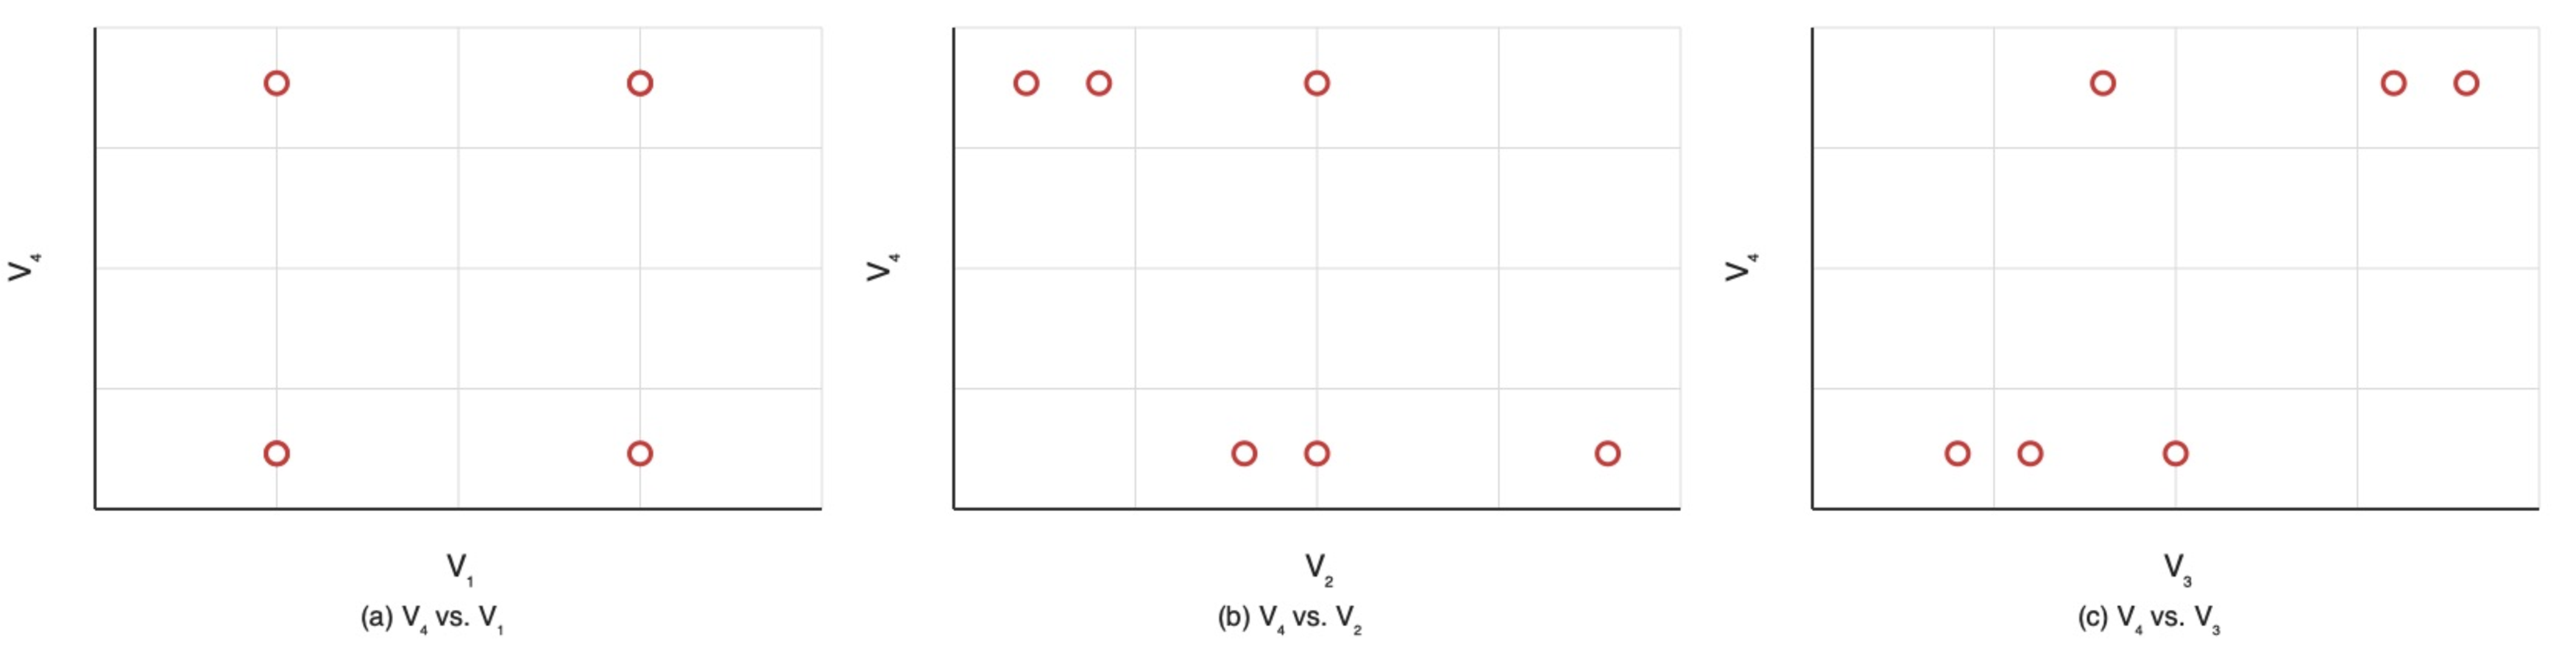
\includegraphics[width=1\linewidth,height=\textheight,keepaspectratio,alt={Three scatter plots comparing the binary fourth variable with each of the first three variables.}]{chapters/../assets/figures/chapter01/scatter-individual.pdf}

}

\caption{\label{fig-data-plot1}Scatter plots: \(V_4\) vs.~\(V_1\),
\(V_2\), and \(V_3\).}

\end{figure}%

Now that the scatter plots hardly reveal any obvious relation, we may
start to look at the interplay of multiple variables. We may ask, for
example, "is the boolean value of the \(4^{th}\) column in any way
associated with the relation between the first two columns?" To answer
this question, we may create a scatter plot of the \(1^{st}\) and
\(2^{nd}\) columns while color-coding the \(4^{th}\). When we do the
same for \(2^{nd}\) vs.~\(3^{rd}\) and \(1^{st}\) vs.~\(3^{rd}\) as
well, we get Figure~\ref{fig-data-plot2}.

\begin{figure}

\centering{

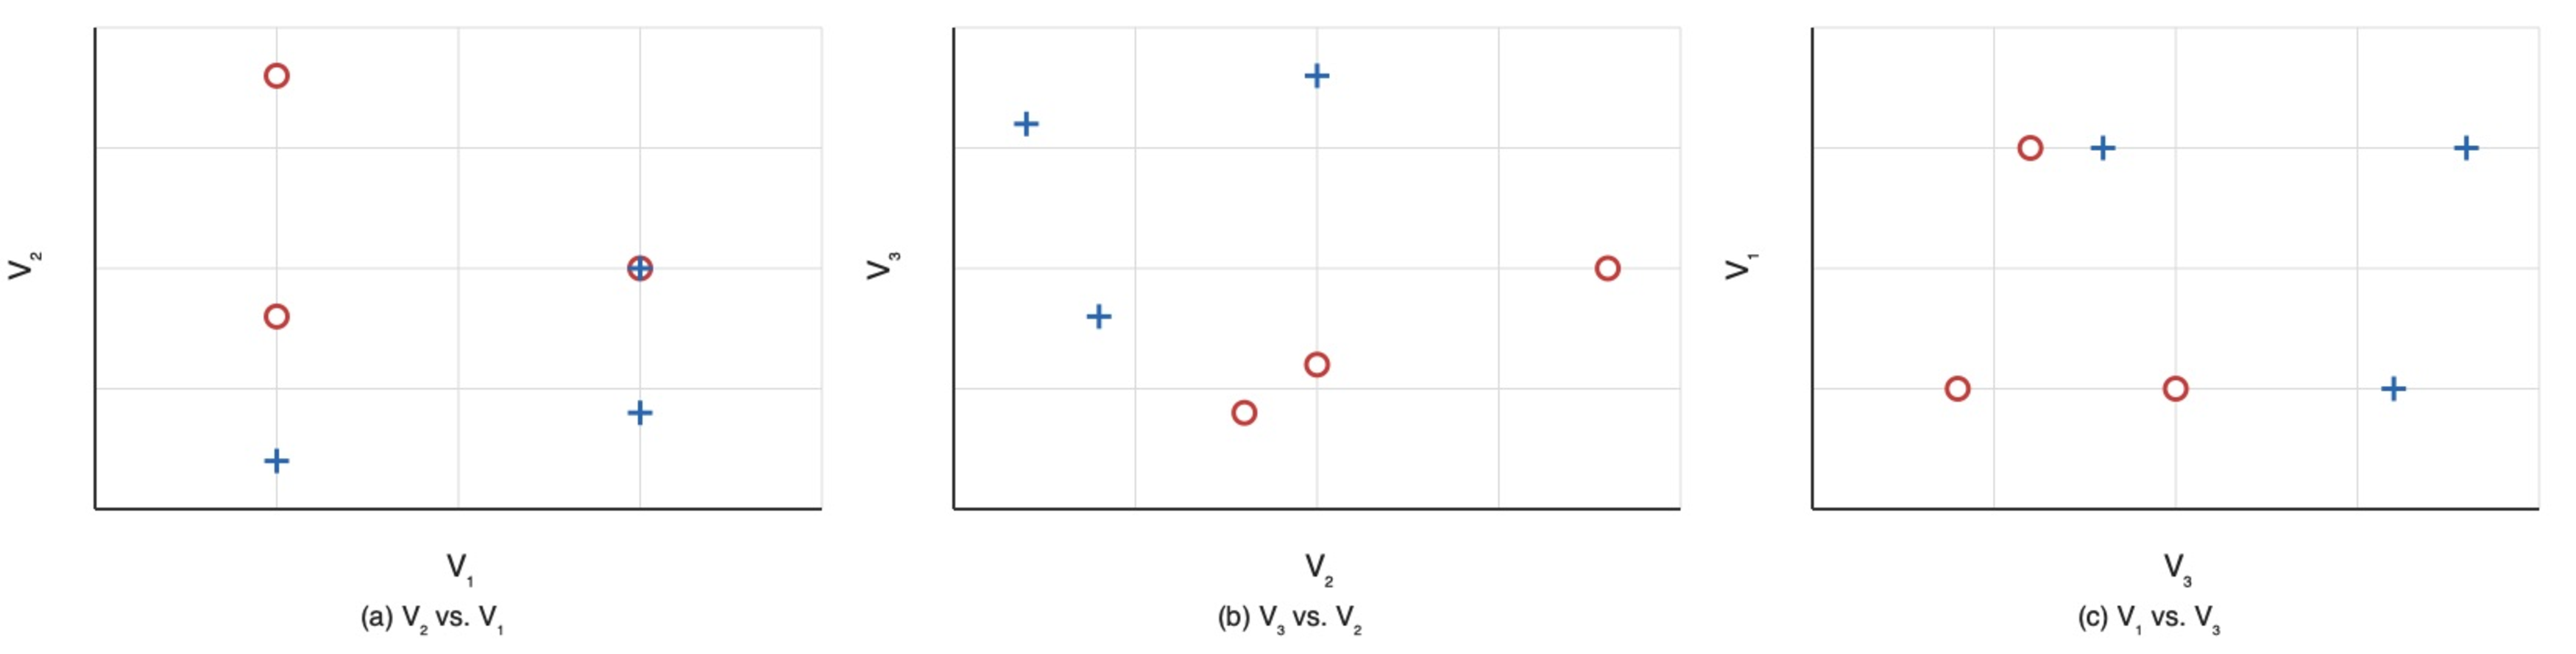
\includegraphics[width=1\linewidth,height=\textheight,keepaspectratio,alt={Three pairwise scatter plots. The middle panel clearly separates red circles below the diagonal from blue plus signs above it.}]{chapters/../assets/figures/chapter01/scatter-pairs.pdf}

}

\caption{\label{fig-data-plot2}Pairwise scatter plots with the value of
\(V_4\) encoded by symbol and color. Red circles represent \(0\); blue
plus signs represent \(1\).}

\end{figure}%

It appears the data are nicely separated in terms of \(4^{th}\) column
values in Figure~\ref{fig-data-plot2} (b), showing the scatter plot of
the \(3^{rd}\) vs.~\(2^{nd}\) column. When the value of the \(3^{rd}\)
column is greater than the value of the \(2^{nd}\), it is \(1\) in the
\(4^{th}\) column; otherwise, it gives \(0\). This can be written as:

\begin{equation}\protect\phantomsection\label{eq-data-ne}{
V_4 = \left\{
\begin{array}{l l}
  1     & if\ V_3 > V_2 \\
  0     & otherwise
\end{array}
\right.
}\end{equation}

This appears to be the pattern so far and can be further verified when
we receive more data. Ultimately, if this is consistent with the
underlying relation in the data -- as far as we can tell from sufficient
data we can receive -- we can claim to have discovered a pattern or new
"knowledge", which is essentially what we have learned in the process of
analyzing the data.

In the machine learning context, we refer to the result of learning,
i.e.~the new "knowledge", as the \emph{concept}.
Equation~\ref{eq-data-ne} is a rule-based approach to concept
representation (descriptor). Sometimes, a (linear) equation may also be
used to represent the result of learning. In this example, equation
\(V_3 - V_2 = 0\) is the straight line that separates the \(0\) and
\(1\) values of column \(4\), as shown in Figure~\ref{fig-data-plot3}.

\begin{figure}

\centering{

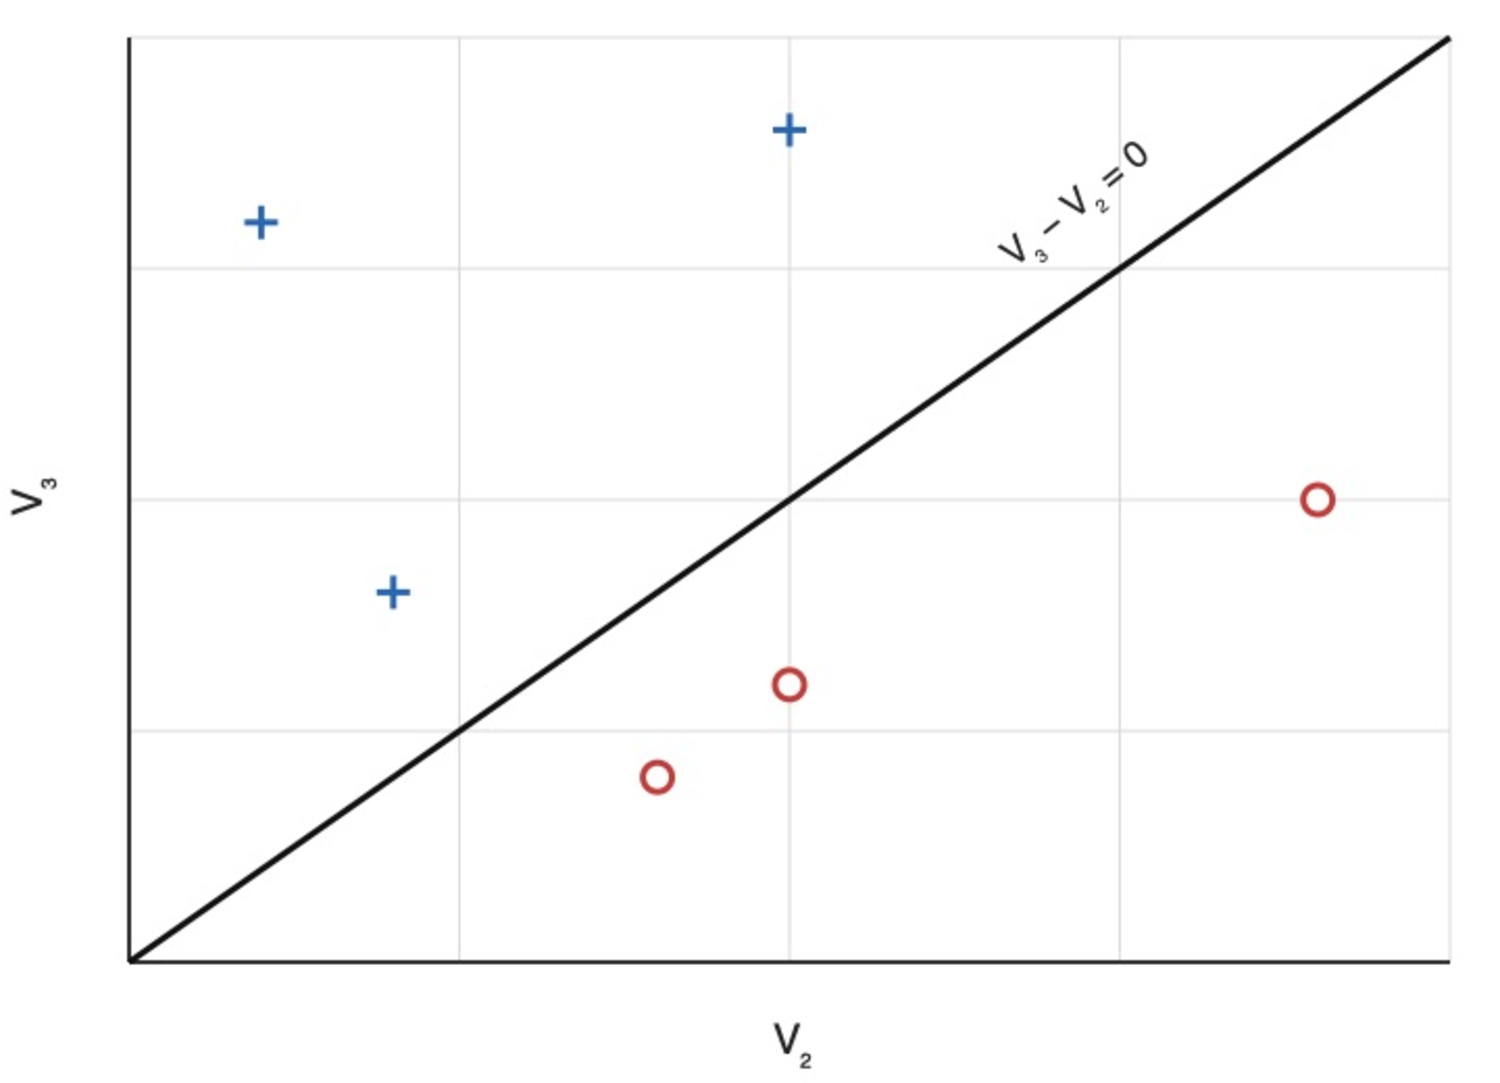
\includegraphics[width=0.7\linewidth,height=\textheight,keepaspectratio,alt={Scatter plot of V3 against V2 with red circles below a diagonal separator and blue plus signs above it.}]{chapters/../assets/figures/chapter01/linear-separator.pdf}

}

\caption{\label{fig-data-plot3}Separating \(0\) vs.~\(1\) in \(V_4\)
with the linear equation \(V_3 - V_2 = 0\).}

\end{figure}%

Whether the concept representation is based on the rules in
Equation~\ref{eq-data-ne} or the linear equation in
Figure~\ref{fig-data-plot3}, it can be identified by computing and
comparing values in the data. Normally such concept representation is
discovered through \emph{training data} and to be applied on testing
data, where decisions or predictions will be made.

\section{Concept Generalizability}\label{concept-generalizability}

The example shows that we can potentially identify a concept and gain
new knowledge by crunching numbers in the data. This could be done
without understanding what the data mean in context. It is important,
however, to examine the representativeness of training data and the
generalizability of concept representation thus learned in the
application domain.

To give the above example some context, the data are in fact about a
collection of shapes, each of which has a number of sides, a width, a
height, and a code indicating whether the shape is \emph{standing} or
\emph{lying}.

\protect\phantomsection\label{tab-data-shapes}
\begin{longtable}[]{@{}cccc@{}}
\caption{Shapes data with column information}\tabularnewline
\toprule\noalign{}
\# Sides & Width & Height & Standing? \\
\midrule\noalign{}
\endfirsthead
\toprule\noalign{}
\# Sides & Width & Height & Standing? \\
\midrule\noalign{}
\endhead
\bottomrule\noalign{}
\endlastfoot
3 & 4 & 2 & 0 \\
4 & 5 & 9 & 1 \\
3 & 9 & 5 & 0 \\
3 & 2 & 4 & 1 \\
4 & 1 & 8 & 1 \\
4 & 5 & 3 & 0 \\
... & .\ldots{} & .\ldots{} & . \\
\end{longtable}

\protect\phantomsection\label{tab-data-shapes}{}

Data in Table~\hyperref[tab-data-shapes]{1.3} represent the shapes shown
in Figure~\ref{fig-data-shapes}. Intuitively, the \emph{concept} of
standing can be understood as describing a human-like object -- when a
person stands, her height is greater than the width; when one lies down,
the horizontal measurement (width) becomes relatively greater.

\begin{figure}

\centering{

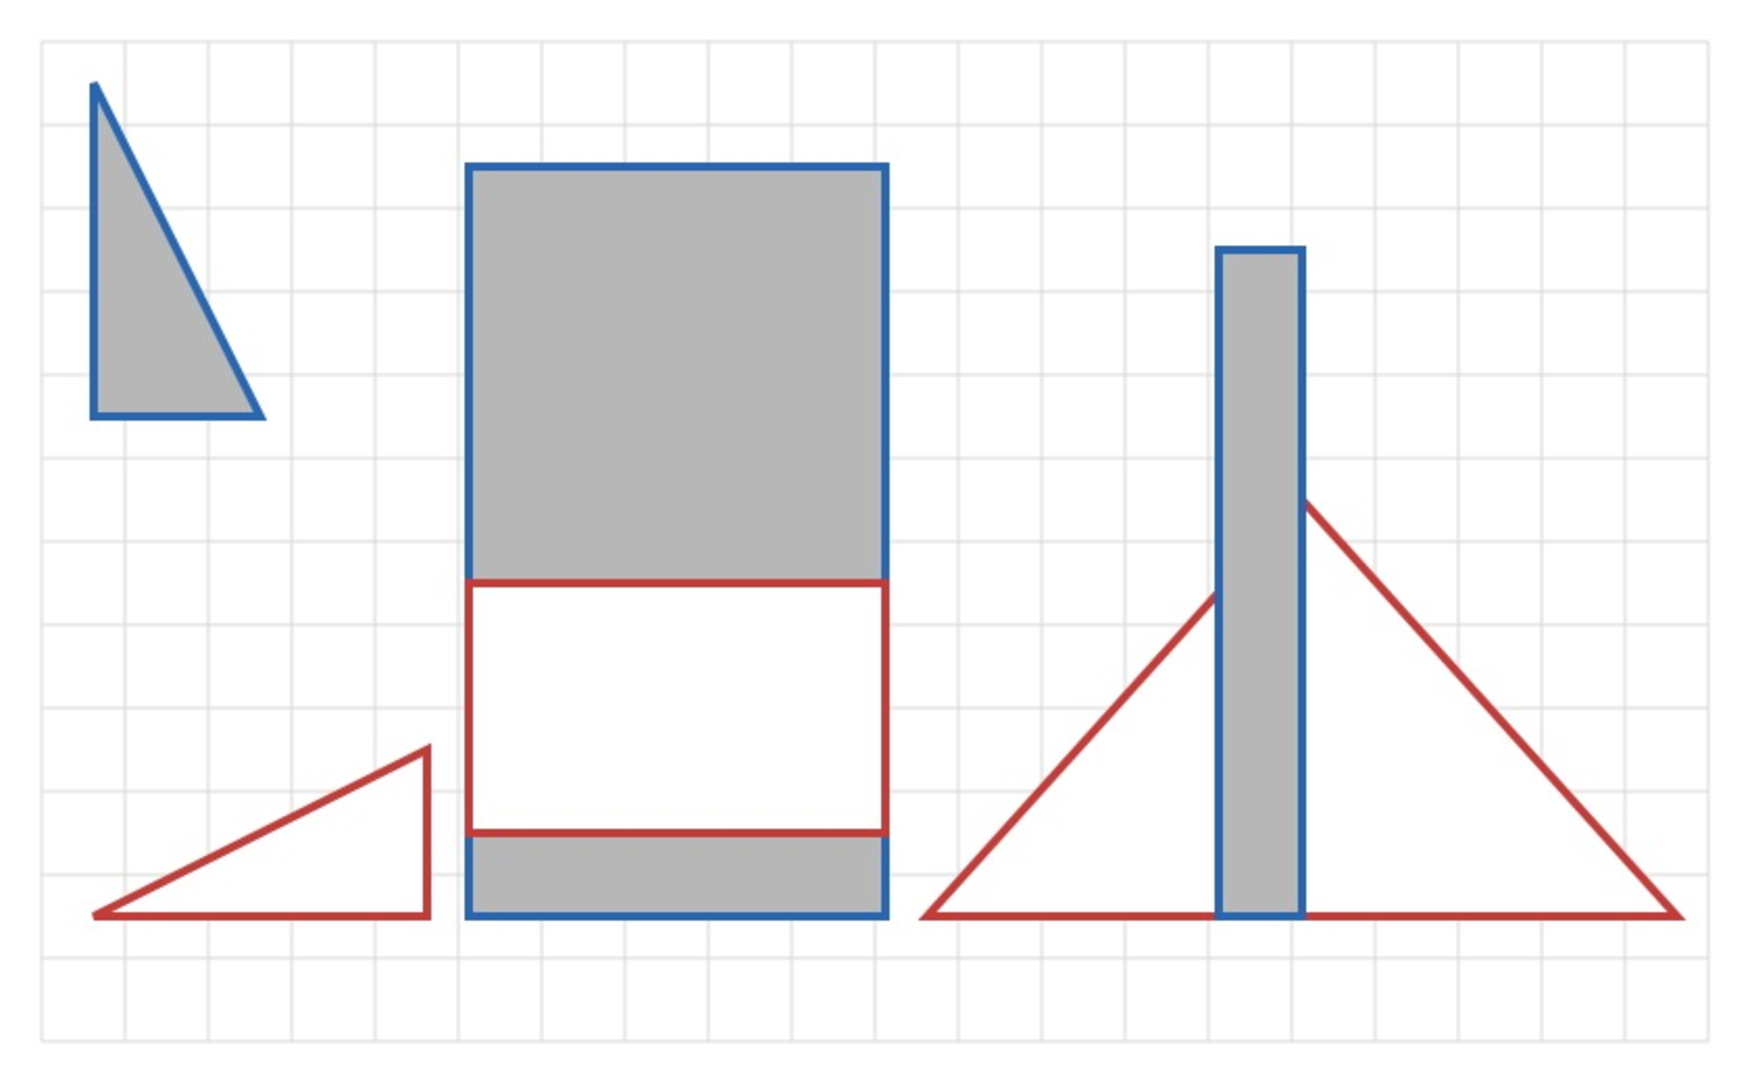
\includegraphics[width=0.75\linewidth,height=\textheight,keepaspectratio,alt={Six triangles and rectangles on a grid. Tall gray shapes are standing; wide white shapes are lying.}]{chapters/../assets/figures/chapter01/shape-examples.pdf}

}

\caption{\label{fig-data-shapes}Shapes of different numbers of sides,
widths, and heights, based on the shapes data. Gray shapes are
classified as \emph{standing}.}

\end{figure}%

It is in this context of human-like shapes that the concept of standing
is injected into the data and can be discovered by mining. It is also in
this context -- again the assumption of human-like shapes -- that the
identified relation of width vs.~height can be applied to related data
for predictions, decision making, etc.

With related assumptions attached, the concept does not represent
universal truth. The same notion of \emph{standing} might be very
different with a more complex shape or structure. In
Figure~\ref{fig-data-building}, for example, the shape of a building may
be flat in terms of its height-width ratio but we see it \emph{standing
as an architecture}.

\begin{figure}

\centering{

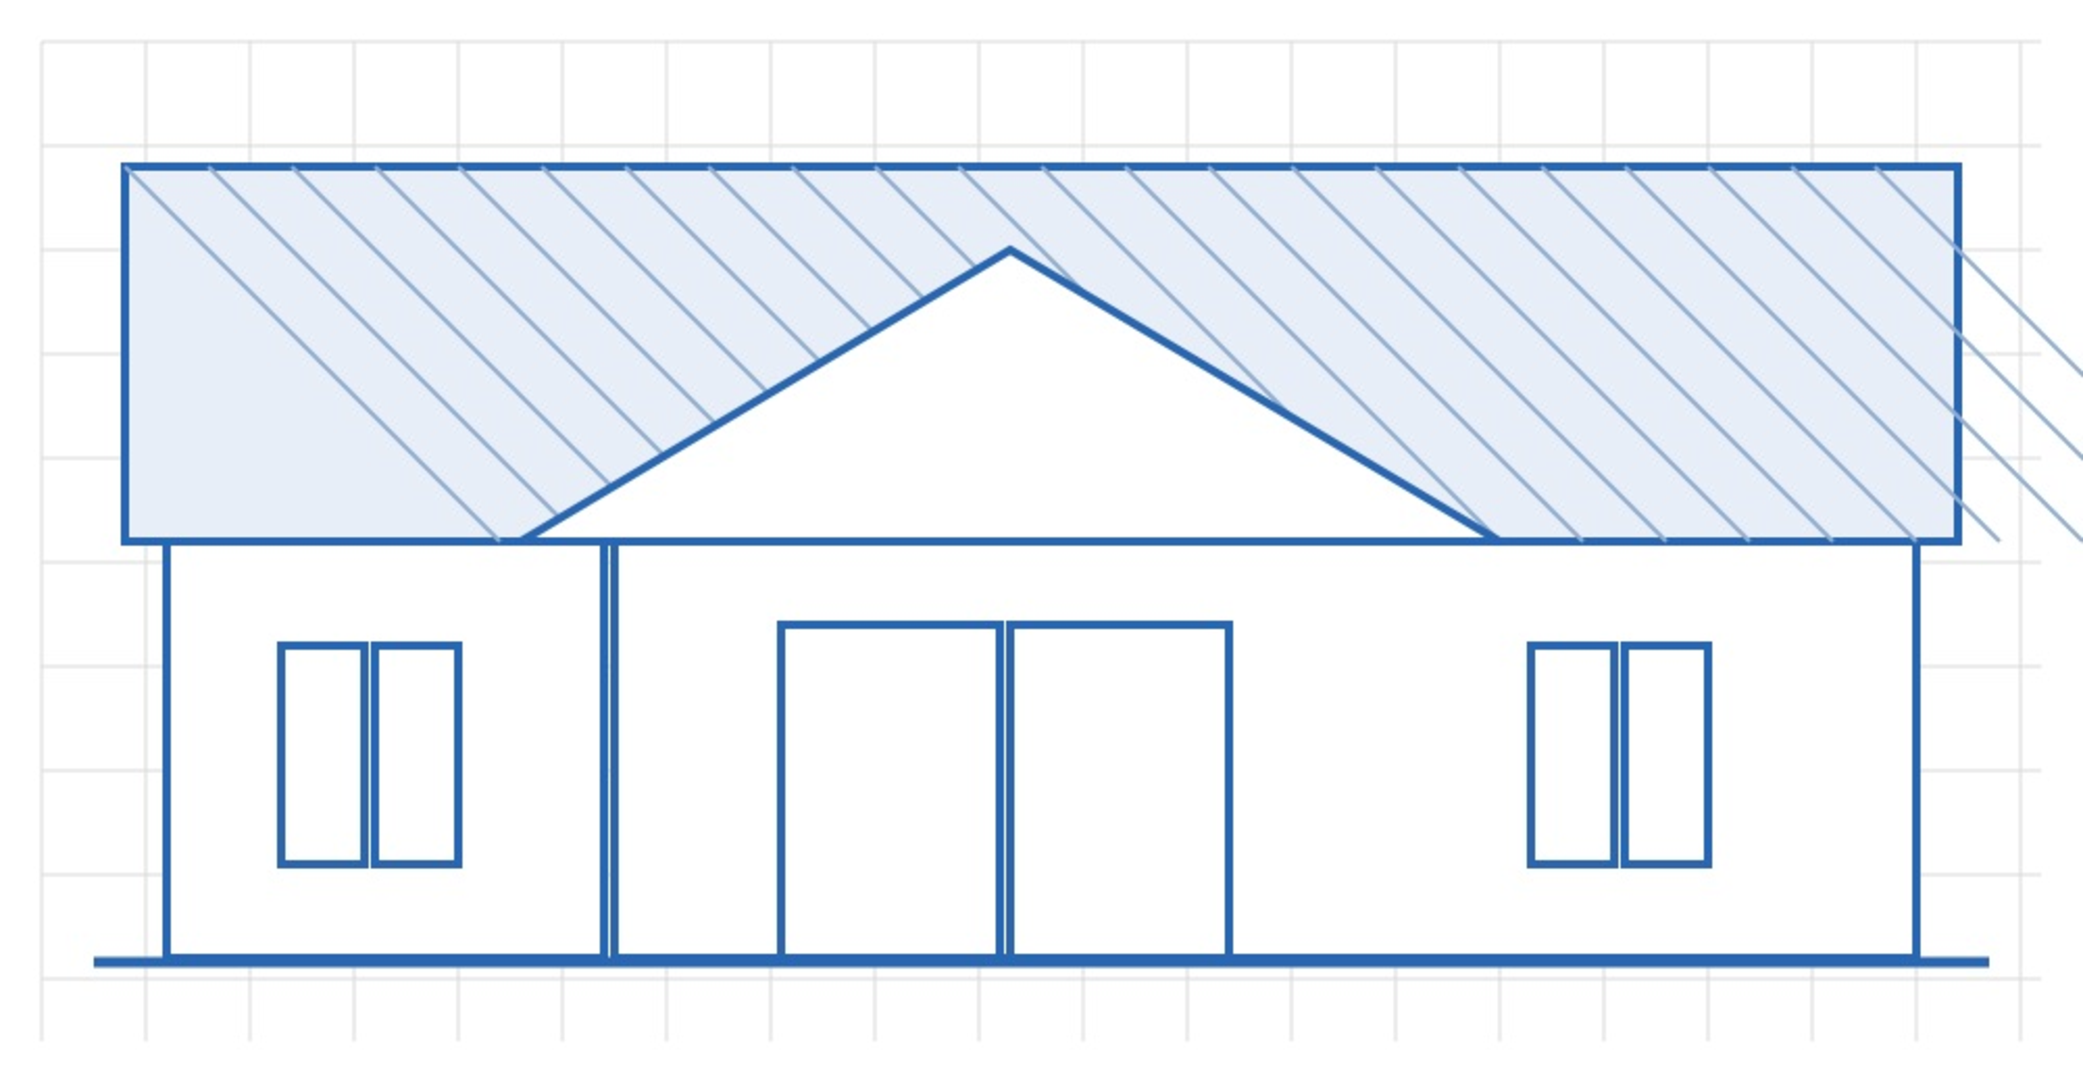
\includegraphics[width=0.75\linewidth,height=\textheight,keepaspectratio,alt={A wide, low building with a roof, doors, and windows on a measurement grid.}]{chapters/../assets/figures/chapter01/standing-building.pdf}

}

\caption{\label{fig-data-building}A \emph{standing} architecture.}

\end{figure}%

It takes an in-depth analysis with proper evaluation and interpretation
to assess the learned concept, its generalizability, and applicability.
This cannot be accomplished by crunching the numbers alone. It requires
human intelligence along with machine learning.

\section{Final Observation}\label{final-observation}

For the concept of \emph{standing}, it turns out that the number of
sides of a shape has no impact on the classification. Variables
(features) as such can be safely removed for the analysis. As far as the
specific concept goes, these variables are part of the noise in the data
and can be identified through feature selection.

The example also shows that it is sometimes (often) insufficient to
model a \emph{concept} on \emph{individual} variables. In the shapes
data example, the concept of \emph{standing} is a relation between the
\emph{width} and \emph{height}. For now, it is a simple, linear
function. Nonetheless, a more complex concept with messier real-world
data may require a non-linear model.\footnote{For example, a non-linear
  model can be a polynomial function. Sometimes, it can also be a linear
  function based on a non-linear transformation of the original data.}
In the following chapters, we will be looking at approaches by which
relations of various complexity can be discovered.

Ultimately, machine learning on massive data may help us identify
patterns and relations that cannot be eye-spotted, which will then lead
to new insight and meaning. And the gained knowledge, if understood
properly, will hopefully result in better decision making and improved
productivity.

\chapter{Data Types and
Representations}\label{data-types-and-representations}

As we employ computers to crunch the data to find meaning and insight,
we need to understand the basic form of data, their basic types and
implications.

\section{Datum}\label{datum}

\subsection{Numerical}\label{numerical}

To compute is to reckon with numbers. Ultimately, all data should be
provided as or transformed into numbers: real numbers, integers or
decimal values.

Consider the mileage of a car \(A\), such as \(96\) thousand miles or,
if one demands to be more precise, \(96,123.5\) miles. Compared to
another car \(B\) at \(64\) thousand miles, one can reasonably make the
following statements:

\begin{enumerate}
\def\labelenumi{\arabic{enumi}.}
\item
  Car \(A\) has a greater mileage than \(B\) has;
\item
  Car \(A\) has \(32\) thousand more miles than \(B\) has;
\item
  The mileage of car \(B\) is \(\frac{2}{3}\) of that of \(A\).
\end{enumerate}

The \(1^{st}\) statement can be made because all numbers can be
compared, e.g.~\(96>64\). However, the \(2^{nd}\) and \(3^{rd}\)
statements make sense because of special characteristics of the
\emph{mileage} variable here.

In fact, we can make the \(3^{rd}\) statement because mileage is a
\emph{ratio-scaled} variable, for which the zero point is well defined.
In this example, a \(0\) mileage corresponds to the fact that the car
has not been driven at all since its production, and is therefore
measured absolutely zero. On such a ratio-scaled variable, many
mathematical operations such as subtraction, addition, and division can
be performed.

Conversely, a temperature variable in Fahrenheit or Celsius is not
ratio-scaled, because a \(0\) value in either \(^{\circ}F\) or
\(^{\circ}C\) is no indication of "zero temperature" or no heat at all.
In this case, we cannot perform addition on its values to get a "total
temperature" or division to obtain a ratio. Nonetheless, related
temperature values are \emph{interval-scaled} because they are measured
in equal units and a distance (difference) between two values is
meaningful.

It is reasonable to say that \(100^{\circ}F\) is \(40\) degrees higher
than \(60^{\circ}F\). As an interval-scaled variable, one can perform
subtraction to compute the distance (interval). The sum (addition),
however, does not have a clear meaning (except as an intermediary step
to calculate the average).

There are also variables for which the unit of measurement is not
necessarily equal or consistent. On a likert scale, for example, rating
numbers from 1 to 5 may be associated with levels of customer
satisfaction, e.g.~extremely unsatisfied to extremely satisfied.
Arguably, the difference between 1 (extremely unsatisfied) and 2
(unsatisfied) may not be the same as that between 3 (moderately
satisfied) and 4 (satisfied). In this case, one can compare the
satisfaction values and rank them. But it is not as meaningful -- at
least not consistent -- to compute and compare their intervals
(differences).

Such a variable is considered \emph{ordinal} as it can be arranged in a
meaningful order but lacks an equal unit of measurement to be
interval-scaled. While we can compare its values, one should refrain
from performing subtraction on them. Neither is addition meaningful with
an ordinal variable.

\subsection{Categorical}\label{categorical}

Ordinal variables are in fact categorical. The values are discrete
numbers to be compared and ranked; but other than that, no mathematical
operations can be performed on them. In fact, they do not have to be
numbers. For example, an \emph{Education} variable with values such as
\emph{high school}, \emph{college}, and \emph{graduate} can be compared
and ranked. These are named values with an order.

A categorical variable can have named values (labels or categories)
without an order. We refer to such variables as \emph{nominal}, of which
values are from a set of \emph{names} or \emph{labels}. The very basic
form of a nominal variable is a binary one, where there are two possible
named values: true or false, yes or no, 0 or 1, etc.

For many variables, these labels are discrete, mutually exclusive
choices without an explicit relation. For example, a \emph{State}
variable can have values such as \emph{PA} and \emph{NY}, and there is
no relation between \emph{PA} and \emph{NY}. One cannot establish such
relation as \(PA>NY\) or \(NY>PA\) unless another variable such as state
population is considered. This type of variable is purely categorical,
not ordinal. With a categorical variable, we can only use the equality
operator to determine whether two values are equal or not, e.g.~is
\emph{PA} the same or different from \emph{NY}.

\section{Data}\label{data}

\subsection{Sets}\label{sets}

We have discussed categorical variables with values from a set of
labels. A set is a collection of member objects or elements. The
elements can be any unique entities, symbols, names, and/or numbers. The
number of elements in a set is referred to as its \emph{cardinality}.

Consider the skill sets of two data science teams A and B:

\[\begin{aligned}
A & = & \{AI, Math, Python, SQL\} \\
B & = & \{InfoVis, Math, R, SQL, Stats\}
\end{aligned}\]

It is easy to count the number of skills in each team and identify their
cardinalities: \(|A|=4\) and \(|B|=5\).

\begin{figure}

\centering{

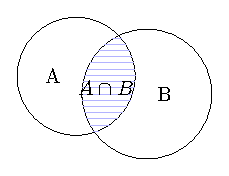
\includegraphics[width=0.45\linewidth,height=\textheight,keepaspectratio,alt={Two overlapping circles labeled A and B, with their intersection shaded.}]{chapters/../assets/figures/chapter02/fig-num-overlap.pdf}

}

\caption{\label{fig-num-overlap}Intersection \(A \cap B\).}

\end{figure}%

The common skill set of the two teams is their \emph{intersection}:

\[\begin{aligned}
A \cap B & = & \{Math, SQL\} \\
|A \cap B| & = & 2
\end{aligned}\]

which is illustrated by the shaded area in Figure~\ref{fig-num-overlap}.
The intersection operation is communicative, i.e.~\(A \cap B=B \cap A\),
because the order does not matter.

Now, if we are to put the two team together on one project, the overall
skill set of the merged project team will be the \emph{union} of the
two:

\[\begin{aligned}
A \cup B
& = & \{AI, InfoVis, Math, Python, R, SQL, Stats\}
\end{aligned}\]

\begin{figure}

\centering{

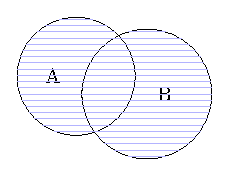
\includegraphics[width=0.45\linewidth,height=\textheight,keepaspectratio,alt={Two overlapping circles labeled A and B, with both circles shaded.}]{chapters/../assets/figures/chapter02/fig-num-union.pdf}

}

\caption{\label{fig-num-union}Union \(A \cup B\).}

\end{figure}%

In this case, the cardinality of the union is:

\[\begin{aligned}
|A \cup B|
& = & |A| + |B| - |A \cap B| \\
& = & 4 + 5 - 2 \\
& = & 7
\end{aligned}\]

Because a set contains only \emph{unique} elements, those in the
intersection \(A \cap B\) will have duplicates when two sets are
combined and should be removed with \(- |A \cap B|\).

The union operation is also communicative, i.e.~\(A \cup B = B \cup A\),
because it does not matter whether we add B to A or A to B. In addition,
both the union and intersection operations have the associative
property, that is:

\[\begin{aligned}
(A \cup B) \cup C & = & A \cup (B \cup C) \\
(A \cap B) \cap C & = & A \cap (B \cap C)
\end{aligned}\]

for any sets A, B, and C. As illustrated in Figure~\ref{fig-num-union3},
we will obtain the same union set (the shaded circles) regardless of
which two are combined first. The same is true with intersection, as
illustrated in Figure~\ref{fig-num-overlap3}.

\begin{figure}

\centering{

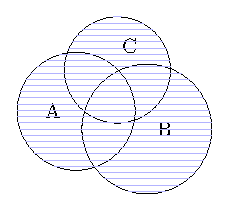
\includegraphics[width=0.45\linewidth,height=\textheight,keepaspectratio,alt={Three overlapping circles labeled A, B, and C, all shaded.}]{chapters/../assets/figures/chapter02/fig-num-union3.pdf}

}

\caption{\label{fig-num-union3}Union of three sets.}

\end{figure}%

\begin{figure}

\centering{

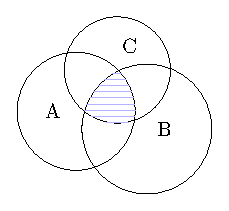
\includegraphics[width=0.45\linewidth,height=\textheight,keepaspectratio,alt={Three overlapping circles labeled A, B, and C, with the common intersection shaded.}]{chapters/../assets/figures/chapter02/fig-num-overlap3.pdf}

}

\caption{\label{fig-num-overlap3}Intersection of three sets.}

\end{figure}%

The union (\(\cup\)) operation is similar to \emph{addition} (\(+\)),
whereas the intersection \(\cap\) operation can be likened to
\emph{multiplication} (\(\times\)). For demonstration, let's look at a
couple of special cases. Let \(0\) denote an empty set, with no elements
at all; \(1\) be the the universal set, containing all elements in the
universe.

For a regular set \(A\), we can show the similarity between union
(\(\cup\)) and addition (\(+\)):

\[\begin{aligned}
A \cup 0  & = & A + 0 \\
          & = & A \\
1 \cup 0  & = & 1 + 0 \\
          & = & 1 \\
1 \cup A  & = & 1 + A \\
          & \approx & 1
\end{aligned}\]

The union of a set A and an empty set \(0\) is the A itself:
\(A \cup 0=A\). The same is true about adding an empty set \(0\) to the
universal set \(1\). \(1 \cup A\) is not exactly \(1 + A\), but they are
roughly the same as long as the universal set \(1\) is far greater than
A.

Likewise, intersection (\(\cap\)) and multiplication (\(\times\))
operations are similar in that:

\[\begin{aligned}
A \cap 0  & = & A \times 0 \\
          & = & 0 \\
1 \cap 0  & = & 1 \times 0 \\
          & = & 0 \\
A \cap 1  & = & A \times 1 \\
          & = & A
\end{aligned}\]

\begin{figure}

\centering{

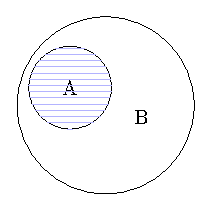
\includegraphics[width=0.45\linewidth,height=\textheight,keepaspectratio,alt={A small shaded circle A entirely contained in a larger circle B.}]{chapters/../assets/figures/chapter02/fig-num-sub.pdf}

}

\caption{\label{fig-num-sub}Subset \(A \subseteq B\).}

\end{figure}%

The intersection between any set (A or 1) and an empty set 0 is always
an empty set: \(A \cap 0 = 0\) and \(1 \cap 0=0\). The intersection
between a set A and the universal set \(1\) is A, because the universal
includes A as a subset. In fact, for any set A that is a subset of B
(see Figure~\ref{fig-num-sub}), their intersection is A and their union
is B:

\[\begin{aligned}
A \cap B & \stackrel{\forall A \in B}{=} & A \\
A \cup B & \stackrel{\forall A \in B}{=} & B
\end{aligned}\]

Besides union and intersection operators that can be likened to addition
and multiplication, there is also the subtraction operator on sets. For
two sets \(A\) and \(B\), \(A-B\) computes the difference between A and
B, or the elements of A that do not appear in B. This is essentially the
removal of their intersection from set A, as shown in
Figure~\ref{fig-num-minus}.

\begin{figure}

\centering{

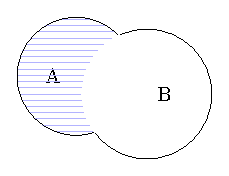
\includegraphics[width=0.45\linewidth,height=\textheight,keepaspectratio,alt={Two overlapping circles labeled A and B, with only the portion of A outside B shaded.}]{chapters/../assets/figures/chapter02/fig-num-minus.pdf}

}

\caption{\label{fig-num-minus}Set subtraction \(A-B\).}

\end{figure}%

The cardinality of the subtracted set can be computed by:

\[\begin{aligned}
  |A-B| & = & |A| - |A \cap B|
\end{aligned}\]

If A and B have no intersection, \(A-B\) is the same as A. If A is a
subset of B, then the result is an empty set. Subtraction is not
communicative, as \(A-B \ne B-A\).

\subsection{Vectors}\label{vectors}

In geometrical terms, a \emph{vector} is an entity having both magnitude
(length) and direction, in a vector space with multiple dimensions.

\begin{figure}

\centering{

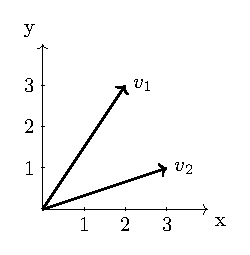
\includegraphics[width=0.65\linewidth,height=\textheight,keepaspectratio,alt={Coordinate plane with vectors from the origin to two points, v1 and v2.}]{chapters/../assets/figures/chapter02/fig-num-vectors.pdf}

}

\caption{\label{fig-num-vectors}Two-dimensional vector space.}

\end{figure}%

Figure~\ref{fig-num-vectors} shows data \(v_1\) and \(v_2\) in a space
with \(X\) and \(Y\) dimensions. In the vector space, each data point is
a vector from the origin \((0,0)\), as shown as directed lines in
Figure~\ref{fig-num-vectors}, and can be represented by its dimensional
values:

\[\begin{aligned}
v_1 & = & (2,3) \\
v_2 & = & (3,1)
\end{aligned}\]

So in this representation, a vector is simply a list of its coordinate
values, each of which represents a feature dimension (variable). The
greater the number of dimensions, the longer the list of the values.

A \emph{set} can be represented by a vector. For example, suppose
\(\{\)AI, InfoVis, Math, Python, R, SQL, Stats\(\}\) is a comprehensive
set of skills for data science teams. Given the A and B teams and their
skills we discussed earlier, we can have the following tabulated binary
representation:

{\def\LTcaptype{none} % do not increment counter
\begin{longtable}[]{@{}lccccccc@{}}
\toprule\noalign{}
Team & AI & InfoVis & Math & Python & R & SQL & Stats \\
\midrule\noalign{}
\endhead
\bottomrule\noalign{}
\endlastfoot
A & 1 & 0 & 1 & 1 & 0 & 1 & 0 \\
B & 0 & 1 & 1 & 0 & 1 & 1 & 1 \\
\end{longtable}
}

where \(0\) represents absence of a skill and \(1\) denotes presence of
the skill. By populating the 0 and 1 values in a fixed order of the
skills, we obtain the vector representations for teams A and B identical
to Table~\hyperref[tab-num-teams]{{[}tab-num-teams{]}}:

\[\begin{aligned}
  A^T     & = & \begin{pmatrix} 1 & 0 & 1 & 1 & 0 & 1 & 0 \end{pmatrix} \\
  B^T     & = & \begin{pmatrix} 0 & 1 & 1 & 0 & 1 & 1 & 1 \end{pmatrix}
\end{aligned}\]

where the vector space has \(7\) dimensions, which correspond to seven
skills in the comprehensive set, to represent instances of data science
teams. These vectors are \emph{row vectors} as they represent data rows.

Note we use superscripted \(A^T\) and \(B^T\), where \(T\) is the
\emph{transpose} operator, because of the convention of using column
vectors by default. By transposing the column vectors A and B -- with a
\(90^\circ\) counterclockwise rotation -- we obtain the row vectors
\(A^T\) and \(B^T\):

\[\begin{aligned}
\begin{matrix}
  A^T     & = & \begin{pmatrix} 1 \\ 0 \\ 1 \\ 1 \\ 0 \\ 1 \\ 0 \end{pmatrix}^T
          & = & \begin{pmatrix} 1 & 0 & 1 & 1 & 0 & 1 & 0 \end{pmatrix}
  \\
  \\
  B^T     & = & \begin{pmatrix} 0 \\ 1 \\ 1 \\ 0 \\ 1 \\ 1 \\ 1 \end{pmatrix}^T
          & = & \begin{pmatrix} 0 & 1 & 1 & 0 & 1 & 1 & 1 \end{pmatrix}
\end{matrix}
\end{aligned}\]

Here, each column vector is a column with \(7\) rows of \emph{real}
numbers. Hence, \(A \in \mathbb{R}^m\) and \(B \in \mathbb{R}^m\), where
\(m=7\). By transposing the column vectors, we obtain row vectors, each
of which has \(m\) columns of \emph{real} numbers.

\chapter{Vectors, Matrices, and Geometric Thinking}\label{ch-matrix}

When we have multiple row vectors of data instances, they form a data
matrix. For example, a data matrix of the two teams \(A^T\) and \(B^T\)
can be represented as \(D\):

\[\begin{aligned}
    D   & = &
    \begin{pmatrix}
        1 & 0 & 1 & 1 & 0 & 1 & 0 \\
        0 & 1 & 1 & 0 & 1 & 1 & 1
    \end{pmatrix}
\end{aligned}\]

Here \(D\) is an \(n \times m\) matrix, with \(n=2\) rows and \(m=7\)
columns. That is, \(D \in \mathbb{R}^{n\times m}\), where \(n=2\) and
\(m=7\). In \(D\), we not only have row vectors for the teams but also
column vectors for the skills:

\[\begin{aligned}
\begin{matrix}
  AI & InfoVis & Math & Python & R & SQL & Stats \\
  = \begin{pmatrix} 1 \\ 0 \end{pmatrix} &
  = \begin{pmatrix} 0 \\ 1 \end{pmatrix} &
  = \begin{pmatrix} 1 \\ 1 \end{pmatrix} &
  = \begin{pmatrix} 1 \\ 0 \end{pmatrix} &
  = \begin{pmatrix} 0 \\ 1 \end{pmatrix} &
  = \begin{pmatrix} 1 \\ 1 \end{pmatrix} &
  =\begin{pmatrix} 0 \\ 1 \end{pmatrix}
\end{matrix}
\end{aligned}\]

\section{Basic Matrix Operation}\label{basic-matrix-operation}

Consider another data set about the annual revenue and profit of three
companies. Let \(X\) be last year's data (in million dollars):

\[\begin{aligned}
    X   & = &
    \begin{matrix}
        x_1 \\
        x_2 \\
        x_3
    \end{matrix}
    \begin{pmatrix}
        3 & 0.5 \\
        20 & 1.5 \\
        12 & 1
    \end{pmatrix}
\end{aligned}\]

where each row is a 2-dimensional vector and can be visualized in
Figure~\ref{fig-matrix-x}.

\begin{figure}

\centering{

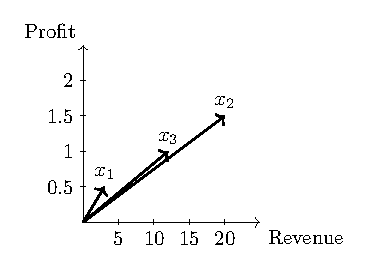
\includegraphics[width=0.6\linewidth,height=\textheight,keepaspectratio,alt={Three vectors representing company revenue and profit in a two-dimensional coordinate plane.}]{chapters/../assets/figures/chapter03/fig-matrix-x.pdf}

}

\caption{\label{fig-matrix-x}Row vectors of matrix \(X\).}

\end{figure}%

Let \(Y\) be this year's data as follow, which, likewise, can be
visualized as \(3\) row vectors in Figure~\ref{fig-matrix-y}:

\[\begin{aligned}
    Y   & = &
    \begin{matrix}
        y_1 \\
        y_2 \\
        y_3
    \end{matrix}
    \begin{pmatrix}
        6 & 1 \\
        15 & 1 \\
        16 & 2
    \end{pmatrix}
\end{aligned}\]

\begin{figure}

\centering{

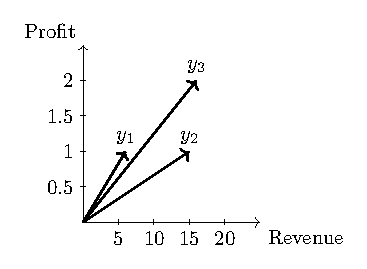
\includegraphics[width=0.6\linewidth,height=\textheight,keepaspectratio,alt={Three updated company vectors in a two-dimensional coordinate plane.}]{chapters/../assets/figures/chapter03/fig-matrix-y.pdf}

}

\caption{\label{fig-matrix-y}Row vectors of matrix \(Y\).}

\end{figure}%

Apparently, \(X\) and \(Y\) have the same dimensionality --
\(X \in \mathbb{R}^{3\times2}\) and \(Y \in \mathbb{R}^{3\times2}\) --
as they are about the same three companies (rows) and two variables
(columns). We can perform simple computation such as addition and
subtraction on the matrices.

For example, it is easy to compute the increase or decrease in revenue
and profit with subtraction:

\[\begin{aligned}
    G
    & = & Y - X   \\
    & = &
    \begin{pmatrix}
        6 & 1 \\
        15 & 1 \\
        16 & 2
    \end{pmatrix}
    -
    \begin{pmatrix}
        3 & 0.5 \\
        20 & 1.5 \\
        12 & 1
    \end{pmatrix} \\
    & = &
    \begin{pmatrix}
        6 - 3 & 1 - 0.5 \\
        15 - 20 & 1 - 1.5 \\
        16 - 12 & 2 - 1
    \end{pmatrix} \\
    & = &
    \begin{matrix}
        g_1 \\
        g_2 \\
        g_3
    \end{matrix}
    \begin{pmatrix}
        3 & 0.5 \\
        -5 & -0.5 \\
        4 & 1
    \end{pmatrix}
\end{aligned}\]

Matrix \(G\), the result of the subtraction, contains data about growth
(increases and decreases). The rows of matrix \(G\) are vectors
connecting respective \(X\) vectors to \(Y\) vectors. Let's single out
the \(3^{rd}\) company from the data, i.e.~\(x_3\), \(y_3\), and
\(g_3\). As shown in Figure~\ref{fig-matrix-xy}, subtraction
\(g_3=y_3-x_3\) is the vector that starts at \(x_3\) and ends at
\(y_3\).

\begin{figure}

\centering{

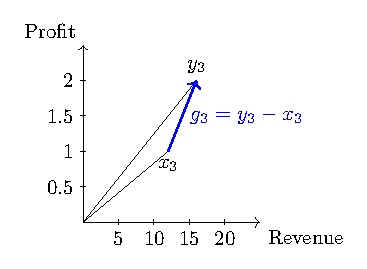
\includegraphics[width=0.6\linewidth,height=\textheight,keepaspectratio,alt={Vectors x3 and y3 connected by their difference vector g3.}]{chapters/../assets/figures/chapter03/fig-matrix-xy.pdf}

}

\caption{\label{fig-matrix-xy}Subtraction geometry.}

\end{figure}%

Suppose the rate of growth in \(G\) is projected to continue (the same)
next year. This will double the growth, which can be computed by:

\[\begin{aligned}
    G \times 2 & = &
    \begin{pmatrix}
        3 & 0.5 \\
        -5 & -0.5 \\
        4 & 1
    \end{pmatrix}
    \times 2 \\
    & = &
    \begin{pmatrix}
        3 \times 2 & 0.5 \times 2 \\
        -5 \times 2 & -0.5 \times 2 \\
        4 \times 2 & 1 \times 2
    \end{pmatrix} \\
    & = &
    \begin{pmatrix}
        6 & 1 \\
        -10 & -1 \\
        8 & 2
    \end{pmatrix}
\end{aligned}\]

\begin{figure}

\centering{

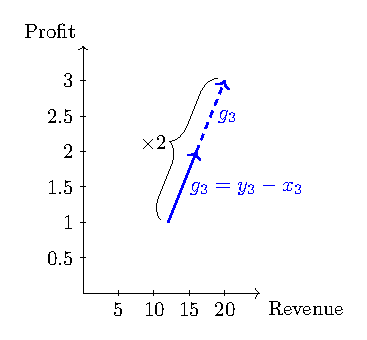
\includegraphics[width=0.6\linewidth,height=\textheight,keepaspectratio,alt={Growth vector g3 and a vector in the same direction with twice its length.}]{chapters/../assets/figures/chapter03/fig-matrix-2g.pdf}

}

\caption{\label{fig-matrix-2g}Geometry of \(g_3 \times 2\), as part of
scalar multiplication \(G\times2\).}

\end{figure}%

Here every value in matrix \(G\) is doubled; so is every vector -- row
or column -- in the matrix. For example, Figure~\ref{fig-matrix-2g}
shows when \(g_3\), the growth vector of the \(3^{rd}\) company (row),
multiplies \(2\), the vector doubles its length (magnitude) in the same
direction. Multiplying a matrix with a scalar (single number) results in
a matrix of the same dimensionality, in which every value is multiplied
by the same scalar. Note the multiplication can be written as
\(2 \cdot G\), \(2G\) or, more generally, \(aG\) given a scalar \(a\)
and a matrix \(G\).

Now with the projected growth (or decrease) data in the \(2G\) matrix,
we can add them to the last year's data matrix \(X\) to compute the
final projection for next year \(Z\):

\[\begin{aligned}
Z & = & Y + 2G \\
  & = &
  \begin{pmatrix}
      3 & 0.5 \\
      20 & 1.5 \\
      12 & 1
  \end{pmatrix}
  +
  \begin{pmatrix}
      6 & 1 \\
      -10 & -1 \\
      8 & 2
  \end{pmatrix} \\
  & = &
  \begin{pmatrix}
      3 + 6 & 0.5+1 \\
      20-10 & 1.5-1 \\
      12 + 8 & 1 + 2
  \end{pmatrix} \\
  & = &
  \begin{matrix}
      z_1 \\
      z_2 \\
      z_3
  \end{matrix}
  \begin{pmatrix}
      9 & 1.5 \\
      10 & 0.5 \\
      20 & 3
  \end{pmatrix}
\end{aligned}\]

\begin{figure}

\centering{

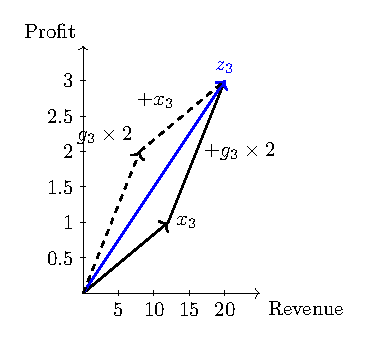
\includegraphics[width=0.6\linewidth,height=\textheight,keepaspectratio,alt={Head-to-tail vector addition showing x3 plus twice g3 resulting in z3.}]{chapters/../assets/figures/chapter03/fig-matrix-z.pdf}

}

\caption{\label{fig-matrix-z}Geometry of addition
\(z_3=x_3 + g_3\times2\).}

\end{figure}%

Note that the data matrix \(Z\) projected from last year's numbers in
\(X\) should be the same as that projected based on this year's data in
\(Y\), i.e.~\(Z=X+2G=Y+G\) given that \(G=Y-X\).

Geometrically, for corresponding vectors in the matrices, the addition
operation is to connect them head to tail. For example, as shown by the
solid lines in Figure~\ref{fig-matrix-z}, for the \(3^{rd}\) row vector,
\(x_3+g_3\times2\) is to connect vectors \(x_3\) and \(2g_3\) and the
result is \(z_3\), which draws from the tail of \(x_3\) to the head of
\(2g_3\). Vector and matrix addition is communicative, the same result
can be obtained by \(2g_3 + x_3\), as shown by dashed lines in
Figure~\ref{fig-matrix-z}.

\section{Sum of Squares}\label{sum-of-squares}

Suppose \(x\) is a m-dimensional column vector, which is essentially a
matrix of \(m\) rows and \(1\) column: \(x \in \mathbb{R}^{m\times1}\).

\[\begin{aligned}
  \begin{matrix}
    x & = &
      \begin{pmatrix}
        x_1 \\
        x_2 \\
        ... \\
        x_m
      \end{pmatrix}
    \end{matrix}
\end{aligned}\]

Now we can transpose the column vector \(x\) into a row vector \(x^T\),
which is a matrix of \(1\) row and \(m\) columns, i.e.
\(x^T \in \mathbb{R}^{1\times m}\):

\[\begin{aligned}
  \begin{matrix}
    x^T & = &
      \begin{pmatrix}
        x_1 &
        x_2 &
        ... &
        x_m
      \end{pmatrix}
    \end{matrix}
\end{aligned}\]

We can multiply \(x^T\) with \(x\) and get their dot product:

\[\begin{aligned}
  \begin{matrix}
    x^Tx & = &
      \begin{pmatrix}
        x_1 &
        x_2 &
        ... &
        x_m
      \end{pmatrix}
      \times
      \begin{pmatrix}
        x_1 \\
        x_2 \\
        ... \\
        x_m
      \end{pmatrix} \\
      & = & x_1^2 + x_2^2 + .. + x_m^2 \\
      & = & \sum_{i=1}^{m} x_i^2
    \end{matrix}
\end{aligned}\]

The result is the total sum of squares, a scalar. Sum of squares is
often performed on error terms in statistical analysis. For example,
given the following errors of three instances:

\[\begin{aligned}
  \begin{matrix}
    e & = &
    \begin{pmatrix}
      0.5 \\
      0.2 \\
      0.7
    \end{pmatrix}
  \end{matrix}
\end{aligned}\]

We can compute the Error Sum of Squares (ESS) by:

\[\begin{aligned}
  \begin{matrix}
    e^Te & = &
      \begin{pmatrix}
        0.5 &
        0.2 &
        0.7
      \end{pmatrix}
      \times
      \begin{pmatrix}
        0.5 \\
        0.2 \\
        0.7
      \end{pmatrix} \\
      & = & 0.5^2 + 0.2^2 + 0.7^2 \\
      & = & 0.78
    \end{matrix}
\end{aligned}\]

\section{Vector Magnitude (Length)}\label{vector-magnitude-length}

Any vector has two components: a direction and a magnitude (length).
Taking the square root of the sum of squares, we can compute a vector's
magnitude:

\[\begin{aligned}
  \begin{matrix}
    \left\lVert x \right\rVert & = & \sqrt{x^Tx} \\
      & = & \sqrt{\sum_{i=1}^{m} x_i^2}
    \end{matrix}
\end{aligned}\]

which is the length from the origin to the data point \(x\). For
example, given a two-dimensional vector \(v\):

\[\begin{aligned}
  \begin{matrix}
    v & = &
      \begin{pmatrix}
        3 \\ 4
      \end{pmatrix}
  \end{matrix}
\end{aligned}\]

Its magnitude can be computed by:

\[\begin{aligned}
  \begin{matrix}
    \left\lVert v \right\rVert & = & \sqrt{3^2 + 4^2} \\
          & = & 5
    \end{matrix}
\end{aligned}\]

\begin{figure}

\centering{

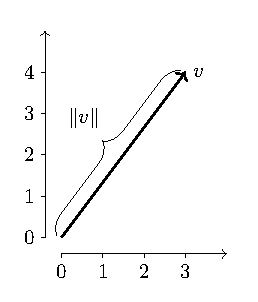
\includegraphics[width=0.55\linewidth,height=\textheight,keepaspectratio,alt={A vector from the origin to the point 3,4, forming a right triangle with length 5.}]{chapters/../assets/figures/chapter03/fig-matrix-magnitude.pdf}

}

\caption{\label{fig-matrix-magnitude}Vector magnitude.}

\end{figure}%

which is the length shown in Figure~\ref{fig-matrix-magnitude}.

\section{Vector Distance}\label{vector-distance}

Let \(y\) be another column vector with the same dimensionality
\(y \in \mathbb{R}^{m\times1}\):

\[\begin{aligned}
  \begin{matrix}
y & = &
  \begin{pmatrix}
    y_1 \\
    y_2 \\
    ... \\
    y_m
  \end{pmatrix}
\end{matrix}
\end{aligned}\]

The difference between \(x\) and \(y\) can be computed by:

\[\begin{aligned}
  \begin{matrix}
x - y & = &
  \begin{pmatrix}
    x_1 \\
    x_2 \\
    ... \\
    x_m
  \end{pmatrix}
  -
  \begin{pmatrix}
    y_1 \\
    y_2 \\
    ... \\
    y_m
  \end{pmatrix}\\
  & = &
  \begin{pmatrix}
    x_1 - y_1 \\
    x_2 - y_2 \\
    ... \\
    x_m - y_m
  \end{pmatrix}
\end{matrix}
\end{aligned}\]

which, geometrically, is the vector connecting the head of \(x\) to that
of \(y\). The magnitude of this difference vector can be computed using
Equation~\hyperref[eq-matrix-magnitude]{{[}eq-matrix-magnitude{]}}:

\[\begin{aligned}
  \begin{matrix}
    \left\lVert x - y \right\rVert & = & \sqrt{(x-y)^T(x-y)} \\
      & = & \sqrt{\sum_{i=1}^{m} (x_i-y_i)^2}
    \end{matrix}
\end{aligned}\]

Consider two two-dimensional vectors:

\[\begin{aligned}
  \begin{matrix}
    u & = &
      \begin{pmatrix}
        2 \\ 1
      \end{pmatrix}
    &
    v & = &
      \begin{pmatrix}
        3 \\ 4
      \end{pmatrix}
  \end{matrix}
\end{aligned}\]

There difference can be computed by:

\[\begin{aligned}
  \begin{matrix}
    v - u & = &
      \begin{pmatrix}
        3 \\ 4
      \end{pmatrix}
      -
      \begin{pmatrix}
        2 \\ 1
      \end{pmatrix} \\
      & = &
        \begin{pmatrix}
          1 \\ 3
        \end{pmatrix}
  \end{matrix}
\end{aligned}\]

\begin{figure}

\centering{

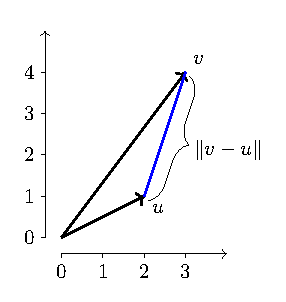
\includegraphics[width=0.55\linewidth,height=\textheight,keepaspectratio,alt={Two vectors from the origin and the difference vector connecting their endpoints.}]{chapters/../assets/figures/chapter03/fig-matrix-distance.pdf}

}

\caption{\label{fig-matrix-distance}Vector distance.}

\end{figure}%

Their Euclidean distance can be computed by the magnitude of their
difference:

\[\begin{aligned}
  \begin{matrix}
    \left\lVert v - u \right\rVert & = & \sqrt{1^2 + 3^2} \\
          & = & \sqrt{10}
    \end{matrix}
\end{aligned}\]

Euclidean distance is symmetric as a metric, i.e.
\(\left\lVert v-u \right\rVert = \left\lVert u-v \right\rVert\). The
distance between the two vectors is illustrated in
Figure~\ref{fig-matrix-distance}.

\section{Vector Angle}\label{vector-angle}

For any vector \(x\), we can factor in its magnitude with
\(\frac{1}{\left\lVert x \right\rVert}\), we obtain its unit vector:

\[\begin{aligned}
  \begin{matrix}
    \hat{x} & = & \frac{x}{\left\lVert x \right\rVert}
    \end{matrix}
\end{aligned}\]

of which the length is normalized to \(1\). We can do the same to
another vector \(y\) to obtain its unit vector:

\[\begin{aligned}
  \begin{matrix}
    \hat{y} & = & \frac{y}{\left\lVert y \right\rVert}
    \end{matrix}
\end{aligned}\]

If \(x\) and \(y\) are both column vectors of the same dimensionality,
\(x \in \mathbb{R}^{m}\) and \(y \in \mathbb{R}^{m}\), we can compute
their dot product by:

\[\begin{aligned}
  \begin{matrix}
    x^Ty & = &
      \begin{pmatrix}
        x_1 &
        x_2 &
        ... &
        x_m
      \end{pmatrix}
      \times
      \begin{pmatrix}
        y_1 \\
        y_2 \\
        ... \\
        y_m
      \end{pmatrix} \\
      & = & x_1 y_1 + x_2 y_2 + .. + x_m y_m \\
      & = & \sum_{i=1}^{m} x_i y_i
    \end{matrix}
\end{aligned}\]

Likewise, we can compute the dot product of their unit vectors:

\[\begin{aligned}
  \begin{matrix}
    \hat{x}^T\hat{y}
      & = &
      \begin{pmatrix}\frac{x}{\left\lVert x \right\rVert}\end{pmatrix}^T
      \begin{pmatrix}\frac{y}{\left\lVert y \right\rVert} \end{pmatrix} \\
      & = & \sum_{i=1}^{m} \frac{x_i}{\left\lVert x \right\rVert} \frac{y_i}{\left\lVert y \right\rVert}
    \end{matrix}
\end{aligned}\]

This turns out to be the cosine of the angle between the two vectors
\(x\) and \(y\):

\[\begin{aligned}
  \begin{matrix}
    cosine(x,y)
      & = &
      \begin{pmatrix}\frac{x}{\left\lVert x \right\rVert}\end{pmatrix}^T
      \begin{pmatrix}\frac{y}{\left\lVert y \right\rVert} \end{pmatrix} \\
      & = & \frac{x^T y}{\left\lVert x \right\rVert \left\lVert y \right\rVert} \\
      & = & \sum_{i=1}^{m} \frac{x_i}{\left\lVert x \right\rVert} \frac{y_i}{\left\lVert y \right\rVert} \\
      & = & \frac{\sum_{i=1}^{m} x_i y_i}{\left\lVert x \right\rVert \left\lVert y \right\rVert}
    \end{matrix}
\end{aligned}\]

Consider the same two vectors discussed earlier:

\[\begin{aligned}
  \begin{matrix}
    u & = &
      \begin{pmatrix}
        2 \\ 1
      \end{pmatrix}
    &
    v & = &
      \begin{pmatrix}
        3 \\ 4
      \end{pmatrix}
  \end{matrix}
\end{aligned}\]

Their magnitudes are:

\[\begin{aligned}
  \begin{matrix}
    \left\lVert u \right\rVert & = & \sqrt{2^2 + 1^2} \\
          & = & \sqrt{5} \\
    \left\lVert v \right\rVert & = & \sqrt{3^2 + 4^2} \\
          & = & 5
    \end{matrix}
\end{aligned}\]

The two vectors can be normalized to unit vectors:

\[\begin{aligned}
  \begin{matrix}
    \hat{u} & = &
      \frac{1}{\sqrt{5}}
      \cdot
      \begin{pmatrix}
        2 \\ 1
      \end{pmatrix}
      & = &
      \begin{pmatrix}
        0.894 \\ 0.447
      \end{pmatrix} \\
    \hat{v} & = &
      \frac{1}{5}
      \cdot
      \begin{pmatrix}
        3 \\ 4
      \end{pmatrix}
      & = &
      \begin{pmatrix}
        0.6 \\ 0.8
      \end{pmatrix}
  \end{matrix}
\end{aligned}\]

\begin{figure}

\centering{

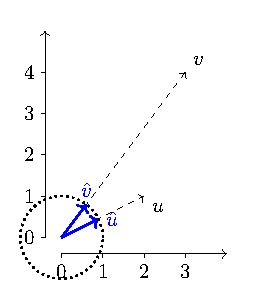
\includegraphics[width=0.6\linewidth,height=\textheight,keepaspectratio,alt={Two vectors and their normalized versions ending on a unit circle.}]{chapters/../assets/figures/chapter03/fig-matrix-unit.pdf}

}

\caption{\label{fig-matrix-unit}Normalization to unit vectors.}

\end{figure}%

As shown in Figure~\ref{fig-matrix-unit}, the normalized unit vectors
\(\hat{u}\) and \(\hat{v}\) point to the same directions of their
original vectors \(u\) and \(v\) respectively. However, the
normalization produce vectors of equal magnitudes. As the dotted circle
shows, the unit vectors are part of a unit circle with radius \(1\).

Please note that we can use a circle to visualize the unit vectors on
the 2-dimensional space (for the 2-dimensional vectors here). For \(3\)
dimensions, we can use a unit sphere for such visualization. For higher
dimensionality, however, we can hardly visualize it but the same idea
holds true mathematically with the notion of \emph{hypersphere}.

Now the dot product of the two unit vectors is:

\[\begin{aligned}
  \begin{matrix}
    \hat{u}^T \hat{v}
      & = &
      \begin{pmatrix}
        0.894 & 0.447
      \end{pmatrix}
      \cdot
      \begin{pmatrix}
        0.6 \\ 0.8
      \end{pmatrix} \\
      & = & 0.894\times0.6 + 0.447\times0.8 \\
      & = & 0.894
  \end{matrix}
\end{aligned}\]

\begin{figure}

\centering{

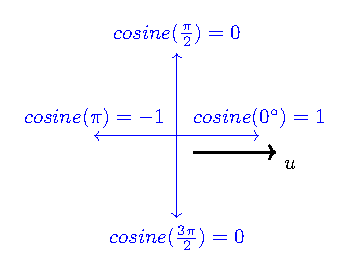
\includegraphics[width=0.6\linewidth,height=\textheight,keepaspectratio,alt={Unit circle diagram showing cosine values for parallel, perpendicular, and opposite vectors.}]{chapters/../assets/figures/chapter03/fig-matrix-cosine.pdf}

}

\caption{\label{fig-matrix-cosine}Cosine values for special angles.}

\end{figure}%

which is the cosine of the angle between \(u\) and \(v\), shown in
Figure~\ref{fig-matrix-unit}. The arc cosine of \(0.894\) corresponds to
an angle of roughly \(27^\circ\) out of a \(360^\circ\) full circle, or
\(0.465\) on a \(2\pi\) scale. Cosine values range between \(-1\) and
\(1\): it is \(1\) when two vector are in the exact same direction
(parallel) and \(-1\) when they are in the opposite direction (a
\(180^\circ\) or \(\pi\) angle). Cosine is \(0\) when two vectors are
orthogonal (perpendicular) to each other (right angle). See
Figure~\ref{fig-matrix-cosine}.

\section{Vector Cross Product}\label{vector-cross-product}

\section{Optimization}\label{optimization}

\section{Kernel Functions}\label{kernel-functions}

\section{Graph Analysis}\label{graph-analysis}

\chapter{Probability and Statistical Thinking}\label{ch-probability}

Probability theory is nothing but common sense reduced to calculation.

\emph{Pierre-Simon Laplace}

In 2012, a national retailer store broke the news by identifying a teen
pregnancy before her father knew about it. After seeing coupons of baby
clothes and cribs sent to his daughter, the enraged father went to the
store to complain about the incident, only to discover later that he was
the one who needed to apologize for his ignorance.

While this story unfolded a spectrum of ethical and privacy-related
issues, we will focus on the technical question for now -- how did the
store figure out the girl was pregnant and it is therefore relevant to
send her baby coupons?

As one can imagine, this was based on the evidence of related purchases
in the girl's shopping history. But even with that, the store could not
be certain about the pregnancy and had to guess how \emph{likely} that
was the case. Computing the \emph{likelihood} or \emph{probability} is
at the core of the technical problem here. We shall look at the basic
theory and rules of \emph{probability} before we can use them to reduce
all this to calculation.

\section{Probability}\label{probability}

\emph{Probability}, according to the Oxford Dictionaries, is "the
quality or state of being probable; the extent to which something is
likely to happen or be the case." While this definition appears common
sense and easy to understand, in reality we use the term
\emph{probability} or likelihood in two very different ways. In the
\emph{Frequentist} view, probability is equivalent to the long-term
frequency of an event's occurrence. Flipping a \emph{perfect} coin, for
example, has a \(50\%\) probability to turn up a head and \(50\%\) tail
because each side has equal chances (frequencies) if it is repeated for
\emph{sufficient} times.

\begin{figure}

\begin{minipage}[t]{0.50\linewidth}

\raisebox{-\height}{

\pandocbounded{\includegraphics[keepaspectratio,alt={Head}]{chapters/../assets/figures/prob/coin_head.png}}

}

\subcaption{\label{}Head}
\end{minipage}%
%
\begin{minipage}[t]{0.50\linewidth}

\raisebox{-\height}{

\pandocbounded{
\includegraphics[keepaspectratio,alt={Tail}]{chapters/../assets/figures/prob/coin_tail.png}}

}

\subcaption{\label{}Tail}
\end{minipage}%

\caption{\label{fig-prob-head-tail}Head versus tail.}

\end{figure}%

On the other hand, the \emph{Bayesian} view of probability is associated
with the degree of belief without complete information or knowledge.
Each coin flipping has nothing to do with a long-term repetition and
which side it turns up is a result of many factors. Likewise, how likely
you are going to get an A on an upcoming test is a belief based on the
known and the unknown -- for example, how well you are prepared and what
questions the test will be comprised of.

These views are rather divided and may lead to different approaches of
modeling and interpretation. Nonetheless, many methods and tools of
great practical values have been derived from both views. And we can
focus on their application without digging deep into the theoretical
subtlety.

\section{Probability Basics}\label{probability-basics}

We denote the probability of an event A's occurrence as \(P(A)\). A
probability is a numeric value between 0 and 1:

\[
0 \le P(A) \le 1
\]

where \(0\) probability means the event will never occur and \(1\), or
\(100\%\), means it will always occur.

Be A the event of turning up a head in a perfect coin flipping,
\(P(A)=\frac{1}{2}\); if A is the event of getting number \(3\) by
rolling a dice, we may estimate \(P(A)\) to be \(\frac{1}{6}\) if we
assume six equal sides without additional information.

The probability of the complement of event A, or that A will NOT occur,
is denoted by \(P(A')\),\footnote{The complementary probability can also
  be denoted by \(P(\bar{A})\), \(P(\neg{A})\) or \(P(A^c)\).} which can
be computed by:

\[\begin{aligned}
P(A') & = & 1 - P(A)
\end{aligned}\]

Head and tail on a coin complement each other. Hence:

\[\begin{aligned}
P(Tail) & = & P(Head') \\
        & = & 1 - P(Head)
\end{aligned}\]

For mutually exclusive events A and B, their union probability, namely
the probability that \emph{either one} of them will occur is the sum of
their individual probabilities:

\[\begin{aligned}
P(A \cup B)
& = & P(A) + P(B)
\end{aligned}\]

\begin{figure}

\centering{

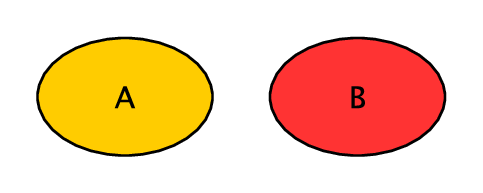
\includegraphics[width=0.45\linewidth,height=\textheight,keepaspectratio,alt={Two separate circles representing events A and B with no overlap.}]{chapters/../assets/figures/prob/p_no_overlap.png}

}

\caption{\label{fig-prob-no-overlap}Mutually exclusive events.}

\end{figure}%

where the symbol \(\cup\) (union) is equivalent to logical OR and
implies addition of the events. When two events are mutually exclusive,
they do not occur simultaneously and, as visualized in
Figure~\ref{fig-prob-no-overlap}, have \emph{no overlap} or intersection
in their probability space. Because of that, we can simply add the two
together.

In the case of flipping a coin, Head and Tail are mutually exclusive. By
the same rule, we have:

\[\begin{aligned}
P(Head \cup Tail)
& = & P(Head) + P(Tail)
\end{aligned}\]

which is \(1\) because Head and Tail complete the entire probability
space. Likewise, numbers \(1\) through \(6\) on a dice are complete,
mutually exclusive events. The same is true that you always get
\emph{one} of the six numbers on a dice:

\[\begin{aligned}
&   & P(1 \cup 2 \cup 3 \cup 4 \cup 5 \cup 6) \\
& = & P(1) + P(2) + P(3) + P(4) + P(5) + P(6) \\
& = & 1
\end{aligned}\]

\section{Joint probability}\label{joint-probability}

If events A and B are not mutually exclusive, their union probability
should be the sum of their probabilities subtracted by the probability
of them occurring simultaneously -- that is the joint probability:

\[\begin{aligned}
P(A \cup B)
  & = & P(A) + P(B) - P(A \cap B)
\end{aligned}\]

\begin{figure}

\centering{

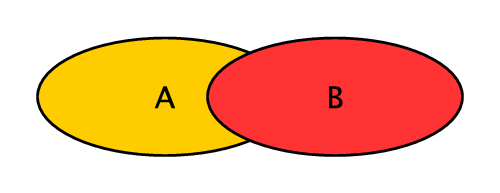
\includegraphics[width=0.45\linewidth,height=\textheight,keepaspectratio,alt={Two overlapping circles representing events A and B.}]{chapters/../assets/figures/prob/p_overlap.png}

}

\caption{\label{fig-prob-overlap}Events that are not mutually
exclusive.}

\end{figure}%

The reason for subtracting the joint probability \(P(A \cap B)\) can be
illustrated in Figure~\ref{fig-prob-overlap}. As shown in the figure,
when A and B can occur simultaneously, they have an overlap
(intersection) which should be discounted so it is not counted
\emph{twice} in the addition.

Here is an example of not mutually exclusive events -- what is the
probability of drawing a card from a deck (52 cards) that is
\emph{either} an Ace (4 out of 52) \emph{or} a Spade (13 out of 52). The
probability of having each can be estimated by:

\[\begin{aligned}
P(Ace) & = & \frac{4}{52} \\
P(Spade) & = & \frac{13}{52}
\end{aligned}\]

\begin{figure}

\centering{

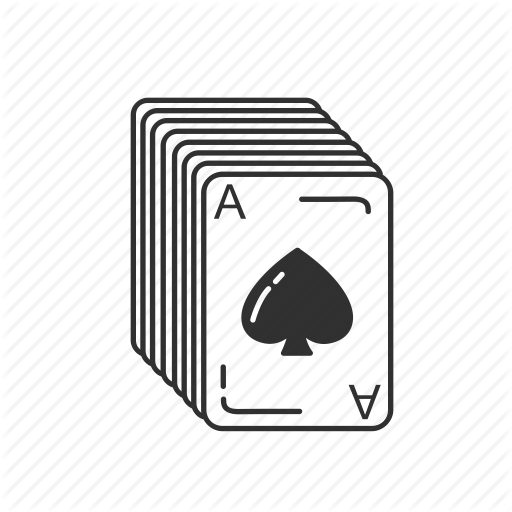
\includegraphics[width=0.35\linewidth,height=\textheight,keepaspectratio,alt={An ace of spades card representing the intersection of aces and spades.}]{chapters/../assets/figures/prob/ace_spades.png}

}

\caption{\label{fig-prob-ace-spade}Ace \(\cap\) spade: a joint (AND)
event.}

\end{figure}%

Because there is \(1\) card that is both an Ace and a Spade, the joint
probability is \(P(Ace \cap Spade) = \frac{1}{52}\) and the union
probability can be computed by:

\[\begin{aligned}
&   & P(Ace \cup Spade) \\
& = & P(Ace) + P(Spade) - P(Ace \cap Spade) \\
& = & \frac{4}{52} + \frac{13}{52} - \frac{1}{52}
\end{aligned}\]

\section{Independent events}\label{independent-events}

Again, the joint probability of A and B, denoted by
\(P(A \cap B)\),\footnote{Joint probability can also be denoted by
  \(P(A, B)\) or P(A AND B).} is the probability that both A and B will
occur.

If A and B are independent, meaning the occurrence of A has nothing to
do with the occurrence of B, then the join probability can be computed
by the simple multiplication:

\[\begin{aligned}
P(A \cap B) & = & P(A) P(B)
\end{aligned}\]

For example, if you flip a coin and roll a dice, how likely will you get
a Head \emph{and} number \(3\). Because the two events are independent,
their joint probability can be computed by:

\[\begin{aligned}
P(Head \cap 3)  & = & P(Head) P(3) \\
                & = & \frac{1}{2} \times \frac{1}{6}
\end{aligned}\]

The joint probability is certainly not limited to two events. You can
apply the same rule to three or more independent events. For a set of
independent events \(E = \{E_1, E_2, .., E_m\}\), their joint
probability is computed by the product of their probabilities:

\[\begin{aligned}
P(E_1 \cap E_2 \cap .. \cap E_m)
& = & \prod_{i=1}^{m} P(E_i)
\end{aligned}\]

Again, the equation holds as long as the events are independent -- that
is, one event's occurrence does not influence the other. While this is
often unrealistic, event independence is often assumed for model
simplicity.

\section{Dependent Events}\label{dependent-events}

Now let's take a step further and look at joint probability of dependent
events. If the occurrence of A is dependent on the occurrence of B, we
can use \(P(A|B)\) to denote the probability of event A \emph{on the
condition that} event B has already been observed. This conditional
probability is referred to as the \emph{posterior probability} because
it is estimated after the fact (here the observation of event B).

The joint probability that both events A and B will occur is then
computed by:

\[\begin{aligned}
P(A \cap B)
& = & P(A|B) P(B)
\end{aligned}\]

where \(P(B)\) is the \emph{prior probability}, which is a priori before
the further observation of data. Again, \(P(A|B)\) is the
\emph{posterior probabilities} conditioned on the observation of the
other event and is about the probability that event A will occur if we
know event B occurs. Likewise, the joint probability can also be
computed by:

\[\begin{aligned}
P(A \cap B)
& = & P(B|A) P(A)
\end{aligned}\]

This is based on the prior probability of and the posterior probability
conditioned on event A. So far the discussion on probability may look
quite abstract. So let's take a look at an example to make sense of
this.

Suppose you are running a restaurant and you look at your transaction
data, and try to learn about the statistics on how to improve your
business. Suppose you find out \(60\%\) of the customers order burgers,
\(54\%\) order burgers and fries. Now you want to know -- if a customer
already orders a burger, how likely he will also order fries. And this
question is certainly relevant to your business.

First let's setup proper notation. Let:

\begin{itemize}
\item
  \(F\) be the event that a customer orders \emph{fries}, and
\item
  \(B\) be the event that a customer orders \emph{burgers}.
\end{itemize}

In this case, you know \(60\%\) of the chance a customer orders burgers,
which is \(P(B) = 0.60\). With \(54\%\) of customers ordering both
burgers AND fries, the joint probability of the two events
\(P(F \cap B) = 0.54\).

Now the question is about the probability of a customer ordering fries
(\(F\)), \emph{on the condition} that she has already ordered a burger
(\(B\)), which is the posterior probability \(P(F|B)\). By replacing A
and B with F and B respectively in
Equation~\hyperref[eq-prob-joint_dep]{{[}eq-prob-joint\_dep{]}}, we
have:

\[\begin{aligned}
P(B) P(F|B) & = & P(F \cap B)
\end{aligned}\]

Divide both sides by P(B), we get:

\[\begin{aligned}
P(F|B)
& = & \frac{P(F \cap B)}{P(B)} \\
& = & 0.54 / 0.60 \\
& = & 0.90
\end{aligned}\]

So it appears the customer will probably (with \(90\%\) probability)
order fries as well if she is ordering a burger.

We can also apply these probability rules to the retailer store story we
discussed at the beginning of the chapter. We can ask questions like --
if a customer has purchased a crib, how likely will she be interested in
coupons of baby clothes? With other related evidence in the shopping
history, can we predict whether the customer is pregnant (or how likely
she is) and, if so, follow up with customized marketing efforts?

\section{The Bayesian Theorem}\label{the-bayesian-theorem}

To attack the above questions, we need to take one step further and look
at the Bayes Theorem.

From equations~\hyperref[eq-prob-joint_dep]{{[}eq-prob-joint\_dep{]}}
and \hyperref[eq-prob-joint_dep2]{{[}eq-prob-joint\_dep2{]}}, we have:

\[\begin{aligned}
P(A|B) P(B)
& = & P(B|A) P(A)
\end{aligned}\]

Divide both sides by \(P(B)\), we get:

\[\begin{aligned}
P(A|B) = \frac{P(A) P(B|A)}{P(B)}
\end{aligned}\]

And with this, we arrive at a very important probability rule, the
\emph{Bayes' Theorem} (rule) on computing posterior probabilities. It is
named after Rev.~Thomas Bayes\footnote{Richard Price helped publish
  Bayes' essay with the formula in 1763, after he passed away. Price, a
  moral philosopher, regarded Bayes Theorem as a means to reason on the
  probability of miracles and to prove the existence of God.} and
further developed by Pierre-Simon Laplace. The rule provides a
foundation for various applications with Bayesian inference and
probabilistic modeling.

\section{Naive Bayes' Model}\label{naive-bayes-model}

Let us look at an application of the Bayes Theorem to get a sense of how
useful the theory is in solving practical problems. One such application
is the Naive Bayes model, which is widely adopted in machine learning,
data mining, and information retrieval. Pay attention to the two
keywords -- \emph{Naive} and \emph{Bayes} -- the model is \emph{Naive}
because the it has naive assumptions about variable \emph{independence},
and is \emph{Bayesian} because the core of the model is the Bayes'
Theorem.

Ultimately, the Naive Bayes model is to estimate the probability of an
inference (hypothesis \(H\)) given observed data (evidence \(E\)), that
is, in the binary scenario, for example, \(P(H|E)\) (true) vs
\(P(H'|E)\) (false). We can compute these probabilities according to the
Bayes' rule:

\[\begin{aligned}
P(H|E) & = & \frac{P(E|H) P(H)}{P(E)} \\
P(H'|E) & = & \frac{P(E|H') P(H')}{P(E)}
\end{aligned}\]

where prior probability \(P(E)\) is the common denominator that does not
differentiate the two and can be ignored for now. \(P(H)\) and \(P(H')\)
can be estimated a priori without evidence \(E\), whereas \(P(E|H)\) and
\(P(E|H')\) can be computed using data observed, in cases when the
hypothesis holds or when it does not.

We shall use a specific example to show how it works. In clinical
diagnosis, a doctor observes a patient's symptoms (evidence) and
determines whether the patient has certain disease (inference /
hypothesis). Chickenpox, for example, exhibits symptoms such as fever
and blisters (rash). Let:

\begin{itemize}
\item
  \(E_1\) denote the symptom of fever, and
\item
  \(E_2\) denote the symptom of blister (rash).
\end{itemize}

The question is how likely the patient has developed chickenpox
(hypothesis \(H\)) if there are symptoms of both fever \(E_1\) and
blisters \(E_2\).

Suppose\footnote{Numbers in the chickenpox example are hypothetical and
  only intended for the sake of computational exercise here.} the
prevalence of chickenpox is \(20\) in every \(1,000\) individuals, that
is \(P(H) = 0.02\) and \(P(H')=0.98\); of those \emph{who develop
chickenpox}, \(90\%\) have fever (\(P(E_1|H)=0.90\)) and \(55\%\) have
blisters (\(P(E_2|H)=0.55\)); of those \emph{without chickenpox}, the
chances of have these individual symptoms are \(P(E_1|H')=0.10\) for
fever and \(P(E_2|H')=0.05\) for blisters.

The first probability we need to attack is \(P(E|H)\), the probability
that a patient exhibiting the observed symptoms \emph{if} she indeed has
chickenpox. Because we consider two symptoms here, this is about the
joint probability when fever and blisters appear simultaneously. With
the \emph{Naive} assumption that the symptoms' occurrences are
statistically independent, \(P(E|H)\) can be computed by:

\[\begin{aligned}
P(E|H)
& = & P(E_1|H) P(E_2|H)
\end{aligned}\]

Put this in
Equation~\hyperref[eq-prob-bayes_he]{{[}eq-prob-bayes\_he{]}} and we
get:

\[\begin{aligned}
P(H|E)
& = & \frac{P(E_1|H) P(E_2|H) P(H)}{P(E)} \\
& = & \frac{0.90 \times 0.55 \times 0.02}{P(E)} \\
& = & \frac{0.0099}{P(E)}
\end{aligned}\]

Likewise, we can compute the probability of a false hypothesis given the
same evidence (symptoms) by:

\[\begin{aligned}
P(H'|E)
& = & \frac{P(E_1|H') P(E_2|H') P(H')}{P(E)} \\
& = & \frac{0.25 \times 0.02 \times 0.98}{P(E)} \\
& = & \frac{0.0049}{P(E)}
\end{aligned}\]

The result shows \(P(H|E) > P(H'|E)\), meaning that it is more likely
than not the patient has developed chickenpox. Again, this model is
based on the Bayes' theorem and the assumption that evidential events
(symptoms) observed are statistically independent. In another word, the
occurrence of one symptom has nothing to do with the other. In reality
we know this independence assumption is rarely true. For example, one
who has blisters is more likely to have fever than those without.

In the above example, we only use two pieces of evidence (symptom
observation) to model the likelihood of chickenpox. In reality, this can
be extended to any number of predictor variables where \(E\) is a set of
variables \(E_1, E_2, .., E_m\) and \(m\) is the size of the set. In
this general case, the Naive Bayesian Model in
equation~\hyperref[eq-prob-bayes_he]{{[}eq-prob-bayes\_he{]}} can be
extended to:

\[\begin{aligned}
P(H|E)  & = & \frac{P(E|H) P(H)}{P(E)} \\
        & = & \frac{P(E_1|H) P(E_2|H)..P(E_m|H) P(H)}{P(E)} \\
        & = & P(H) \prod_{i=1}^{m} P(E_i|H) / P(E)
\end{aligned}\]

Likewise, on the probability of a false hypothesis:

\[\begin{aligned}
P(H'|E)  & = & P(H') \prod_{i=1}^{m} P(E_i|H') / P(E)
\end{aligned}\]

where variables \(E_1, E_2, .., E_m\) are assumed to be statistically
independent. The main purpose of having this naive assumption is for
mathematical simplicity when we compute joint probabilities. Although
this assumption is at odds with reality, related models have turned out
to perform quite well in experiments. Practically the number of
variables (features) \(m\) can be very large. For example, in text
analysis, it is common to treat unique words as individual features
(variables) and, with even a moderate text collection, there can be tens
of thousands, if not millions, of variables in the model.

The Bayes Model is not limited to a binary case, e.g.~chickenpox vs.~not
chickenpox. It can also be applied to any classification problem on a
number of discrete outcomes. In that case, we simply need to compute the
probability of each discrete outcome (hypothesis) and find out which one
has the greatest likelihood. It can also be extended to a continuous
case where numeric predictions can be made based on certain probability
distribution models, which we will discuss later in the chapter.

\section{Probability Estimators}\label{probability-estimators}

Again, consider
Equation~\hyperref[eq-prob-bayes_hem]{{[}eq-prob-bayes\_hem{]}}, in
order to compute the probability of each hypothesis, we need to first
estimate the probability of each evidence \(E_i\) in
\(\prod_{i=1}^{m} P(E_i|H)\). Where do these probabilities come from?
Essentially they are learned from the training data where we can count
their frequencies, or the number of times each unique situation occurs.
For now, the probability \(P(E_i | H)\) is computed by:

\[\begin{aligned}
P(E_i | H) & = & \frac{F(E_i | H)}{F(H)}
\end{aligned}\]

where \(F(E_i | H)\) is the number of instances with \(E_i\) where
hypothesis \(H\) is true and \(F(H)\) is the total number of instances
with the true hypothesis.

Imagine you are working on the problem of email spam detection. You have
a training data set of \(1,000\) emails and \(100\) have been identified
spams (where hypothesis \(H_{spam}\) is true). Suppose \(prize\) is one
of the keywords (evidence \(E_{prize}\)) that can be used to model the
spam detection problem and, of the \(100\) spam emails (\(H_{spam}\))
there are \(20\) containing that keyword \emph{prize}. In this case,
\(F(H_{spam}) = 100\) and \(F(E_{prize} | H_{spam}) = 20\) so, according
to the probability estimator in
equation~\hyperref[eq-prob-pf]{{[}eq-prob-pf{]}}, the probability
\(P(E_{prize} | H_{spam})\) can be computed by:

\[\begin{aligned}
P(E_{prize} | H_{spam})
  & = & \frac{F(E_{prize} | H_{spam})}{F(H_{spam})} \\
  & = & 20 / 100 \\
  & = & 0.2
\end{aligned}\]

This will work just fine as long as the relative frequencies
(occurrences) of related keywords in the training data (\emph{sample})
are proportional to those of the same keywords in all spam emails in the
world (\emph{population}). In this case, we assume what we observe in
the sample data is what will most likely occur in the population.

In reality, however, we may observe data in samples with varied
departures from the entire population. Imagine we want to use
\emph{prize} as one feature in the Naive Bayes but observe no occurrence
at all of this term in the training spam data, that is
\(F(E_{prize} | H_{spam}) = 0\).

In this case, are we to simply conclude the probability of having
\emph{prize} in \emph{any} spam email \(P(E_{prize} | H_{spam})\) is
\(0\)? This is obviously a premature conclusion -- the fact that you
have not seen an \emph{elephant} does not lead you to conclude on the
non-existence of that very creature. There is variance in the data and
we do not want to be misled by data in its departure (skewness) from the
overall reality.

\begin{figure}

\centering{

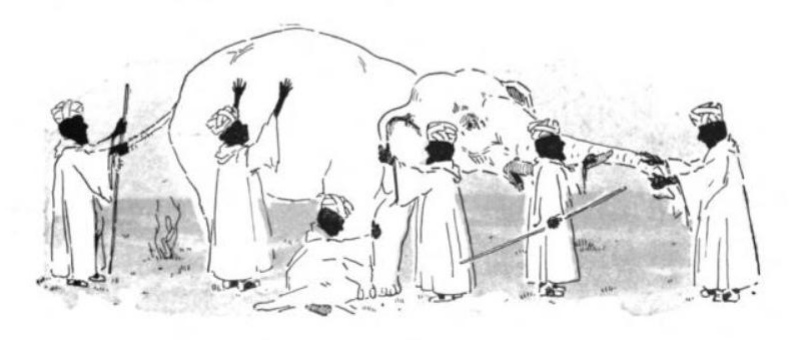
\includegraphics[width=3in,height=\textheight,keepaspectratio]{chapters/../assets/figures/prob/elephant.jpg}

}

\caption{\label{fig-prob-elephant}Blind men and elephant. If you have
not seen an elephant, does it mean there is no elephant? If you only
touch an elephant on its leg, does it mean the elephant is like a tree
trunk? These misperceptions are due to our sample data (where you touch
the elephant) and should be corrected with external knowledge.}

\end{figure}%

Data may be localized, just as the story of \emph{blind men and
elephant} shows (Figure~\ref{fig-prob-elephant}). But we should aim to
see the whole picture.

In addition, there is also an undesired consequence for having a zero
probability in the Naive Bayes model. With \(E_{prize}\) as one of the
evidence features, its probability \(P(E_{prize} | H_{spam})\) is one of
the factors in computing the product in the Bayes equation above. When
\(P(E_{prize} | H_{spam}) = 0\), it leads to \(P(H|E) = 0\) regardless
of the values of other variables.

In short, we have observed that zero probabilities are not desirable,
neither theoretically nor practically. One simple remedy to zero
probability estimates, as suggested by Pierre Laplace, is to add \(1\)
to each frequency (count) in the sample. So the frequency of having term
\(prize\) in the spams becomes:

\[
F(E_{prize} | H_{spam}) + 1
\]

To be fair, we also need to add \(1\) to other frequency counts,
including the frequency of NOT having the term \(prize\) in the spam
subset:

\[
F(E'_{prize} | H_{spam}) + 1
\]

The above two are complete and mutually exclusive cases. Hence, the
total number of instances in the spams becomes:

\[\begin{aligned}
 &   & F(E_{prize} | H_{spam}) + 1 + F(E'_{prize} | H_{spam}) + 1 \\
 & = & F(H_{spam}) + 2
\end{aligned}\]

Note that we add \(2\) to the total number because we have a binary
variable, namely having term \(prize\) (true) vs.~not having it (false).
If a variable has \(k\) discrete values, then we need to add \(k\) to
the total. For example, a categorical variable that marks an email's
importance may have three different levels such as \emph{low},
\emph{normal}, and \emph{high}. If we add \(1\) to the frequency of each
level, in the end we will have added \(3\) to the total.

But the question then is why add \(1\)? In fact the idea is that we can
add any \emph{constant} \(c\) to each count so zero values can be
avoided. And the probability of observing a variable value \(v\) within
the sample where the hypothesis is true can be computed by:

\[\begin{aligned}
P(E_i = v | H) & = & \frac{F(E_i=v | H) + c}{F(H) + kc}
\end{aligned}\]

where \(k\) is the number of discrete values variable \(E_i\) can have,
e.g. \(k=3\) for the email priority variable, and \(c\) is a chosen
constant which represents some prior knowledge about the chance of any
value. A great \(c\) value will make the probability more predetermined
and a lesser value gives relatively more weigh to frequencies observed
in the sample data. When a discrete value occurs less frequently in the
sample, \(c\) will change its probability estimate more dramatically.

In a sense, an added constant \(c\) favors the rare values and penalizes
the frequent ones. Other than simplicity, is this a rational strategy to
estimate the probabilities? The answer depends on how much we know about
the probability distributions with or without the sample data. If in
fact we know some values are going to occur more frequently regardless
-- for example, we can safely assume most emails would have been marked
as \emph{normal} -- then we should add more to its count proportionately
in the sample data. The probability can be estimated by:

\[\begin{aligned}
P(E_i = v | H) & = & \frac{F(E_i=v | H) + c p_v}{F(H) + k c}
\end{aligned}\]

where \(p_v\) is the \emph{a priori} probability of each discrete value
\(v\) (\(v \in [v_1, v_2, .., v_k]\)) and they add up to
\(\sum_v p_v = 1\). The assignment of \(p_v\) values depends on
\emph{prior knowledge}. Practically it is not always clear how they can
be obtained. Besides domain knowledge, training samples are often the
major source where we gather related statistics so the simple
transformation of adding \(1\) or another constant is what works in many
practical applications.

\section{Probability Distributions and
Models}\label{probability-distributions-and-models}

Think about this. The very fact that we have to \emph{normalize} the
obtained frequencies -- to avoid zeros or for other purposes --
indicates that we do not totally trust what observed data (samples) can
tell us about. The underlying assumption is that we have certain
understanding (prior knowledge) about how data should behave and we will
need to \emph{correct} the data whenever they \emph{drift} from that
expected behavior. By doing the normalization or smoothing, we impose a
\emph{model} of expected \emph{probability distributions} on the
analysis.

We shall now prepare us with an introductory discussion of probability
distributions, from discrete to continuous cases.

\begin{figure}

\centering{

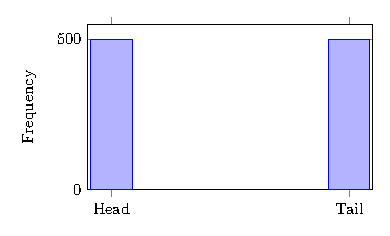
\includegraphics[width=0.55\linewidth,height=\textheight,keepaspectratio,alt={Bar chart with equal frequencies of 500 for heads and tails.}]{chapters/../assets/figures/chapter04/fig-prob-coin-freq.pdf}

}

\caption{\label{fig-prob-coin-freq}Frequency distribution of flipping a
coin: 500 heads versus 500 tails after \(1,000\) trials in the ideal
world.}

\end{figure}%

First let's look at some discrete cases. Imagine you toss a coin for
1000 times and in the perfect world you get 500 heads and 500 tails. And
you can create a simple bar plot to show the frequency distribution of
500 for both heads and tails. This is a uniform distribution because
every event, head vs.~tail, has an equal chance.

\begin{figure}

\centering{

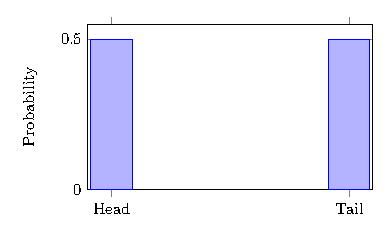
\includegraphics[width=0.55\linewidth,height=\textheight,keepaspectratio,alt={Bar chart with probability 0.5 for heads and 0.5 for tails.}]{chapters/../assets/figures/chapter04/fig-prob-coin-prob.pdf}

}

\caption{\label{fig-prob-coin-prob}Probability distribution of flipping
a coin: heads and tails each have probability \(0.5\).}

\end{figure}%

Now instead of talking about frequencies or counts, we can describe the
distribution in terms of chance (probabilities). And in this case, head
and tail have equal chances (probabilities) of 50\% or 0.5 in the
distribution, as Figure~\ref{fig-prob-coin-prob} shows.

For the sake of discussion, let's extend the binary case, head vs.~tail,
to a larger number of exclusive outcomes. For example, imagine you roll
a dice. If you roll it for a sufficient number of times, the sides will
have equal chances to appear, that is, each side from 1 to 6 has a
probability of 1/6 to occur, as shown in Figure~\ref{fig-prob-dice}.

\begin{figure}

\centering{

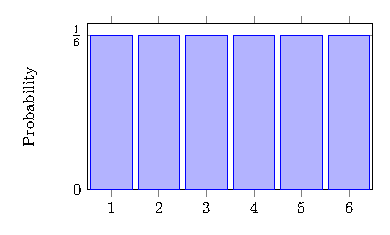
\includegraphics[width=0.65\linewidth,height=\textheight,keepaspectratio,alt={Uniform bar chart assigning probability one sixth to each face from one through six.}]{chapters/../assets/figures/chapter04/fig-prob-dice.pdf}

}

\caption{\label{fig-prob-dice}Probability distribution of rolling a
die.}

\end{figure}%

Two simple but important observations here:

\begin{enumerate}
\def\labelenumi{\arabic{enumi}.}
\item
  The probabilities of the six sides add up to one because they are
  exhaustive, mutually exclusive choices;
\item
  The probability distribution is a uniform distribution as they are all
  equal. The heights of the bars form a flat, horizontal line that
  characterizes the uniform distribution.
\end{enumerate}

\section{Continuous Probability
Distribution}\label{continuous-probability-distribution}

So far these are discrete distributions. But we can extend this to a
continuous distribution. If the outcome \(x\) is no longer limited to
such integers or specific labels. Perhaps the outcome of the question at
hand can be any number in the range of 1 and 6, and you are to predict
that number. If it is a uniform distribution in with the continuous
variable, it remains a flat line in the range of 1 - 6, shown in
Figure~\ref{fig-prob-cont}.

\begin{figure}

\centering{

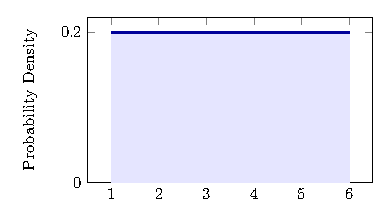
\includegraphics[width=0.65\linewidth,height=\textheight,keepaspectratio,alt={Flat probability-density line between one and six.}]{chapters/../assets/figures/chapter04/fig-prob-cont.pdf}

}

\caption{\label{fig-prob-cont}Probability density of a continuous
variable \(x\).}

\end{figure}%

Again, when we add all probabilities up in the distribution, the total
should still be \(1\). But because this is a continuous space, we are
talking about infinite amount of numbers. The outcome can be number 3 or
any decimal number such as \(3.14159\). To add the infinite number of
heights (some sort of "probability" values) in the distribution is
essentially \emph{integration} of the distribution function (a flat line
in this case), that is, the area under the distribution line or curve.
The result of the integration or the entire area will \emph{always} be
\(1\), as long as the plotted range includes all possible outcomes.

With a uniform (flat) distribution, the area is a rectangle as shown in
Figure~\ref{fig-prob-cont} and it is easy to calculate the area. In the
above case, the area of the rectangle between \(1\) and \(6\) can be
computed by width times height, which is \((6-1) \times 0.2 = 1\). So
this meets the expectation that the sum of the entire probability
distribution is \(1\).

Although the above is discussed as a \emph{probability} distribution, we
shall clarify on an important concept. The uniform height \(0.2\) in
Figure~\ref{fig-prob-cont} is NOT a probability value per se. It is what
we refer to as a \emph{probability density}, but not exactly a
probability. For now, let us move on from the uniform distribution to a
more common distribution in the real world before we come back to
elaborate on the concept of \emph{probability density} again.

In the real world, you do not often see uniform
distributions\footnote{Even in an equal-opportunity society, there is
  rarely any even (uniform) distribution of goods, wealth, etc.}. Normal
(Gaussian) distributions are much more common. For example, if we
collect statistics about adult male heights in the U.S., you will see
the heights are not equally likely. Instead, the overwhelming majority
of (average) people have the average height around 70 inches. And much
rarer are shorter than 62 or taller than 78. The whole distribution is a
bell curve as shown in the figure here.

\begin{figure}

\centering{

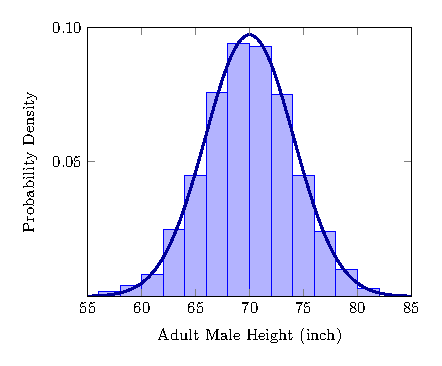
\includegraphics[width=0.65\linewidth,height=\textheight,keepaspectratio,alt={Bell-shaped probability-density curve centered near the average adult male height.}]{chapters/../assets/figures/chapter04/fig-prob-height.pdf}

}

\caption{\label{fig-prob-height}Distribution of adult male heights,
approximately a normal distribution (bell curve).}

\end{figure}%

This is again a probability density distribution so if you integrate the
curve, the total area under it will be \(1\) or \(100\%\) probability.
When you pick a particular number on the \(x\) axis such as \(70\)
inches in the middle, you notice it is \(y = 0.1\) on the distribution
curve. Now be careful that this value \(0.1\) does NOT mean that there
is \(10\%\) chance to be \(70\) inches height (exactly).

Because they are infinite number of values in the range, each exact
height value in fact has a \(0\) probability to occur. The reason is
when we say \(70\) inches, we mean exactly \(70.000000...\) with an
infinite number of decimal zeros. And it is close to \emph{impossible}
to get that exact value on a continuous scale.

Back to the question. So what does a value like \(0.1\) mean on the
\(y\) axis? It means \(0.1\) probability density -- that is, \(0.1\)
probability \emph{per inch} (range) on the adult height scale. And this
value will change if you change the unit of height, for example by
switching to centimeters.

What does this probability density entail now that it is not probability
and it varies on the measuring unit? Probability density does allow you
to compare probabilities of different continuous \emph{values} and
\emph{value ranges}. For example, in the normal distribution here, you
can still tell that the probability of a height \emph{around} \(70\)
inches is greater than that in the proximity of \(80\). But to tell the
exact probability, you will need to specify a range. You can ask the
question of how likely an adult height is \(70\) \emph{something}
(i.e.~between 70 and 71) inches. And you can integrate the area under
the bell curve in the range to find out.

To reiterate this point -- on the simpler example of the uniform
distribution presented in Figure~\ref{fig-prob-cont}, the \(0.2\) value
on y is not probability but probability density or probability per unit.
You can still tell that all probabilities are equal by looking at the
flat line. And you can ask the question about how likely you will get a
value between 2 and 4 by multiplying the density which is \(0.2\) and
the range which is \(2\) and the result turns out to be \(0.4\) -- that
is \(40\%\) of the chance you will get a value \emph{in that range}.

As always, all probabilities add up to \(1\) as you can verify by
\(0.2 \times (6-1) = 1\). So if you ask how likely a value occurs in the
range between \(1\) and \(6\), given the distribution in
Figure~\ref{fig-prob-cont}, the answer is that it will \emph{always be
true}.

There are several major categories of probability distributions beyond
the uniform and normal distributions we discussed here. Some of these
are asymmetric, exhibiting a form of imbalance between the lower and
higher ends. Power-law distributions and their variations, for example,
are very common in many natural and social structures. They are often
associated with basic \emph{counts} in these structures and activities.

The distribution of wealth or income is an example of the power-law
distribution, where the overwhelming majority is \emph{poor} (with
relatively little wealth) and a small percent at the top are extremely
wealthy. This is a result commonly regarded as due to the \emph{Matthew
Effect}\footnote{The term \emph{Matthew Effect} is named after the
  Gospel of Matthew, in which Jesus is recorded as saying, "for to every
  one that hath shall be given, and he shall abound: but from him that
  hath not, that also which he seemeth to have shall be taken away" with
  the parable of the talents.}, in which the rich get rich. In citation
and network analysis, this effect is also known as the \emph{cumulative
advantage}(Price 1976) or \emph{preferential attachment}(Barabási and
Albert 1999).

Spoken language (word frequencies) follows the Zipf law, which can be
regarded as a special case of the power-law distribution.
Figure~\ref{fig-prob-word-freq} shows the distribution of word
frequencies taken from the novel \emph{Moby Dick}. As shown in
Figure~\ref{fig-prob-word-freq} (a), there is a great divide between the
rich and the poor -- a large number of words have only been used once or
twice in the novel (tall bars on the left of the distribution) where
very few words have a frequency higher than \(100\) (the long tail).

It is difficult, however, to examine the long tail on normal coordinates
as the values are very small (low) within a long range. Logarithmic
transformation is often conducted to better visualize the distribution.
The result is Figure~\ref{fig-prob-word-freq} (b), where both \(x\)
(words' occurrences) and \(y\) (frequencies of the occurrences) have
been transformed with logarithm.\footnote{Essentially log-transformation
  reduces a number to its order, e.g. \(1000\) to \(3\) and \(100\) to
  \(2\) with \(log_{10}\).}

\begin{figure}

\begin{minipage}[t]{0.50\linewidth}

\raisebox{-\height}{

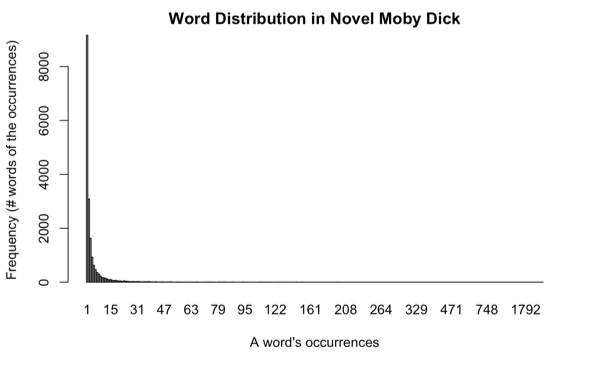
\includegraphics[width=2in,height=\textheight,keepaspectratio,alt={Normal coordinates}]{chapters/../assets/figures/prob/word_freq.png}

}

\subcaption{\label{}Normal coordinates}
\end{minipage}%
%
\begin{minipage}[t]{0.50\linewidth}

\raisebox{-\height}{

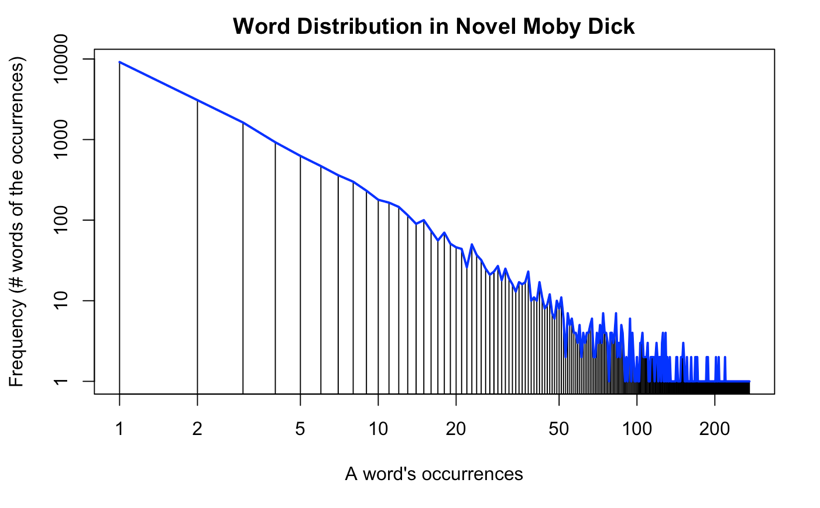
\includegraphics[width=2in,height=\textheight,keepaspectratio,alt={Log-log coordinates}]{chapters/../assets/figures/prob/word_freq_log.png}

}

\subcaption{\label{}Log-log coordinates}
\end{minipage}%

\caption{\label{fig-prob-word-freq}Word frequency distribution}

\end{figure}%

One prominent characteristic of a power-law distribution is that it
follows a straight line on log-transformed coordinates spanning across a
vast range of numeric orders and is therefore considered \emph{scale
free}. One should caution though that many distributions may roughly
look linear with log-transformation when they are in fact the result of
a different distribution. In reality, there are various constraints and
capacity limits on related structures where the outcome is not ideally
power-law. In social networks, for example, even those who are super
active can only maintain up to a certain number of friendly contacts and
therefore the outcome of friendship distribution will be subject to such
human limits and not scale-free.

\section{Probability Estimators}\label{probability-estimators-1}

The first approach we used to compute probability is to follow whatever
the sample data tell us. If we take a sample of \(1000\) emails and
\(300\) of them are spams, the estimated probability is given by
\(300/1000 = 0.3\). If we analyze \(100\) emails and \emph{NONE} of them
have the term \emph{prize} in them, then we are bound to conclude the
probability that we will ever encounter the term is \(0\). This naive
method of trusting whatever in the sample data is part of a spectrum of
methods referred to as the \emph{Maximum Likelihood Estimator} (MLE).

Simply put, an MLE chooses as estimates the values that maximize the
likelihood of the observed sample. In the case of observing \(0\) emails
with term \emph{prize} in the sample, we shall thus estimate the term
never occurs in any email in the whole world (population) so that NOT
observing it is the most likely outcome, which is the case of the
observed sample. In general, for discrete distributions, the result of
an MLE is given by frequencies of related values in the sample without
further transformation.

\subsection{Discrete Probability
Estimation}\label{discrete-probability-estimation}

Now if we have additional knowledge about the domain and can assume
probabilities follow a particular distribution model, then the question
becomes how we can specify parameters of that model to maximize the
probability of the observed data. Suppose among all emails you receive,
you find out for three particular days there are \(5\), \(3\), and \(7\)
emails containing the term \emph{prize} on each day. We assume that:

\begin{itemize}
\item
  The number of such emails you receive one day is independent of that
  on another day. That is, receiving more or less such email today does
  not affect the number you will receive tomorrow and in the future.
\item
  During a small time interval, the probability of receiving such an
  email is proportional to the length of the time interval. That is, the
  longer the time, proportionally greater the probability.
\end{itemize}

Under these conditions, the probability of receiving \(x\) number of
\emph{prize} emails can be modeled by a Poisson probability distribution
and the probability mass function is:

\[\begin{aligned}
P(x) & = & e^{-\mu} \frac{\mu^x}{x!}
\end{aligned}\]

where:

\begin{itemize}
\item
  \(e\) is the Euler constant which is approximately \(2.71828\);
\item
  \(x\) is the number of such emails in question, and \(x!\) is the
  factorial
  \(x!=x \times (x-1) \times (x-2) \times .. \times 2 \times 1\);
\item
  \(u\) is the only parameter, the mean number of \emph{prize} emails,
  to be estimated.
\end{itemize}

With an MLE, we are to maximize the likelihood of obtaining the 3-day
sample, that is the joint probability of having \(5\), \(3\), and \(7\)
emails \(P(x=5 \cap x=3 \cap x=7)\) on three separate days. Now that we
assume the days are independent, the joint probability can be computed
by:

\[\begin{aligned}
  & & P(x=5 \cap x=3 \cap x=7) \\
  & = & P(x=5) P(x=3) P(x=7)
\end{aligned}\]

With the Poisson probability function in
Equation~\hyperref[eq-prob-poisson]{{[}eq-prob-poisson{]}}, this
becomes:

\[\begin{aligned}
  &   & P(x=5 \cap x=3 \cap x=7) \\
  & = & e^{-\mu}\frac{\mu^5}{5!} \times e^{-\mu}\frac{\mu^3}{3!} \times e^{-\mu}\frac{\mu^7}{7!} \\
  & = & \prod_{x \in [5,3,7]} e^{-\mu} \frac{\mu^x}{x!}
\end{aligned}\]

Now MLE of the Poisson distribution is to estimate the only parameter,
the value of mean \(\mu\), so that the above probability in
Equation~\hyperref[eq-prob-point_poisson]{{[}eq-prob-point\_poisson{]}}
is maximized. Now instead of maximizing the product (multiplications) of
the probabilities, we can take the logarithm of
Equation~\hyperref[eq-prob-point_poisson]{{[}eq-prob-point\_poisson{]}},
which becomes:

\[\begin{aligned}
l(\mu) & = & \ln(\prod_{x \in [5,3,7]} e^{-\mu} \frac{\mu^x}{x!}) \\
& = & \sum_{x \in [5,3,7]} \ln(e^{-\mu} \frac{\mu^x}{x!})
\end{aligned}\]

and try to maximize the sum of log likelihood\footnote{With a positive
  variable such as a probability, when its value \(p\) increases, its
  \(log(p)\) always increases. So when \(log(p)\) reaches its maximum,
  so does the \(p\) value. Because of this, we can maximize \(log(p)\)
  in order to maximize \(p\).}. We can do this by taking the derivative
of
Equation~\hyperref[eq-prob-point_poisson_log]{{[}eq-prob-point\_poisson\_log{]}}:

\[\begin{aligned}
l'(\mu) & = & \frac{1}{\mu} \sum_{x \in [5,3,7]} x - n
\end{aligned}\]

where \(n\) is the number of observations of the sample, which is \(3\)
for 3 days. The maximum can be reached with the derivative at \(0\),
which is:

\[\begin{aligned}
  &   & \frac{1}{\mu} \sum_{x \in [5,3,7]} x - 3 \\
  & = & \frac{5+3+7}{\mu} - 3 \\
  & = & 0
\end{aligned}\]

And we can conclude that:

\[\begin{aligned}
\mu & = & (5 + 3 + 7) / 3 \\
    & = & 5
\end{aligned}\]

maximizes the probability of observing the sample data of \(3\), \(5\),
\(7\) on three days following the Poisson distribution. With the
estimate for parameter \(\mu=5\), we can now compute the probability for
any discrete value with
Equation~\hyperref[eq-prob-poisson]{{[}eq-prob-poisson{]}}. For example,
we can find out that it is very unlikely on one day to receive \(10\)
emails containing the term \emph{prize}:

\[\begin{aligned}
  P(x=10)
  & = & e^{-\mu} \frac{\mu^x}{x!} \\
  & = & e^{-5} \frac{5^{10}}{10!} \\
  & \approx & 0.01
\end{aligned}\]

We can also make it a general case that, a Poisson MLE shall estimate
the paramter \(\mu\) based on the sample mean:

\[\begin{aligned}
\mu & = & \bar{x} \\
    & = & \frac{\sum_{i=1}^{n} x_i}{n}
\end{aligned}\]

where \(n\) is the number of observations in the sample data.

\subsection{MLE for a Continuous
Variable}\label{mle-for-a-continuous-variable}

For a continuous variable, we can also assume a specific functional form
of its distribution such as a normal distribution and the objective of
an MLE is to estimate related parameters (e.g.~mean \(\mu\) and variance
\(\delta^2\)) of the distribution function, from which the sample data
are most likely to be observed. These parameter estimates are then used
to compute probability densities at specific values or probabilities
within certain ranges.

Suppose \(X\) is a numeric variable with a normal distribution, the
probability of any value \(x\) is given by the following function:

\[\begin{aligned}
  f(x) & = & \frac{1}{\sqrt{2\pi\delta}} e^{-\frac{(x-\mu)^2}{2\delta^2}}
\end{aligned}\]

This is one of the most recognized formulas in statistics. Although it
looks daunting, there are only two parameters and the rest are
constants, including \(\pi\) the ratio of a circular circumference to
its diameter which is about \(3.14159\). From a sample data of \(n\)
instances, the two parameters, namely mean \(\mu\) and variance
\(\delta^2\), can be estimated by the sample mean and variance:

\[\begin{aligned}
  \hat{\mu} & = & \frac{\sum_{i=1}^{n} x_i}{n} \\
  \hat{\delta^2} & = & \frac{\sum_{i=1}^{n} (x_i - \hat{\mu})^2}{n-1}
\end{aligned}\]

where \(x_i\) is each observed value of \(x\) in the sample data.

Normal distributions are symmetric with the highest probability density
at the very center of the bell curve. Given the objective of MLE to
maximize the likelihood of observed sample, it makes sense that the
parameter estimates should ultimately put the sample data at the center
(so they are more likely to occur). Now that the center is also the mean
of the symmetric distribution, we can now estimate the population mean
using directly the mean of the sample, which is what
Equation~\hyperref[eq-prob-norm_paras]{{[}eq-prob-norm\_paras{]}} does.

\section{Summary}\label{summary}

Because it is probabilistic, we assume there is no absolute certainty.
So any probability estimate is a guess based on the data you have and
best evidence you can identify. There is always a chance it may go
wrong. And so we are not to blindly trust the outcome/prediction of a
model (neither probabilistic nor any other models). In many critical
settings, human machine collaboration is key -- in the medical
environment, there have been retrieval and AI systems that can provide
necessary assistance to technicians and physicians, but they are not
there to take over and do everything for us. That said, we also have to
recognize there are human errors as well. When we think and make
decisions, even as professionals/experts, we cannot be 100 In short, the
point is -- models are not perfect, as humans are. So the best way is to
understand what they are really good at and in what ways we can use
their assistance.

\chapter{Information, Entropy, and Divergence}\label{ch-information}

It from bit.

John Archibald Wheeler

Imagine taking a quiz consisting of \(3\) true/false questions. If one
has not studied the subject, she can take a guess on each of the
questions and there are \(8\) (i.e.~\(2\times2\times2=2^3\)) possible
sets of answers to the entire quiz. Without the ultimate knowledge about
what is correct, each set of answers has a likelihood of \(p = 1/8\) to
be the correct one.

\protect\phantomsection\label{tab-info-quiz}
\begin{longtable}[]{@{}cccccccc@{}}
\caption{All possible sets of answers to a quiz of \(3\) binary
questions. Each answer set has a probability of \(1/8\) to be the
correct one.}\tabularnewline
\toprule\noalign{}
\endfirsthead
\endhead
\bottomrule\noalign{}
\endlastfoot
T & T & T & T & F & F & F & F \\
T & T & F & F & T & T & F & F \\
T & F & T & F & T & F & T & F \\
1 & 2 & 3 & 4 & 5 & 6 & 7 & 8 \\
\end{longtable}

\protect\phantomsection\label{tab-info-quiz}{}

Now if we assume the \(3\) questions are independent (without an overlap
of knowledge), one needs \(3\) piece of information to answer them.
Therefore, the amount of information required to find the correct answer
is proportional to:

\[\begin{aligned}
  H
  & = & 3 \\
  & = & \log_2 2^3 \\
  & = & - \log_2 \frac{1}{8} \\
  & = & - \log_2 p
\end{aligned}\]

where \(p\) is the probability of one out of \(8\) possible outcomes and
the log base \(2\) reflects that fact that each question is binary (true
or false). In the above \(8\) mutually exclusive answer sets, each
represents a choice and adds to the uncertainty of getting the correct
set of answers. Of the overall \(-\log_2 \frac{1}{8}\), each answer set
\(i\) of the \(8\), if treated equally likely, requires the following
amount to be confirmed or eliminated as the ultimate outcome:

\[\begin{aligned}
H_i
& = & - \frac{1}{8} \log_2 \frac{1}{8}
\end{aligned}\]

where \(\frac{1}{8}\) can be regarded as the probability of \(i^{th}\)
outcome \(p_i\):

\[\begin{aligned}
H_i
& = & - p_i \log_2 p_i
\end{aligned}\]

This quantity can be linked to Shannon's information theory, also known
as the Mathematical Theory of Communication, in which the amount of
(missing) information can be measured by the \emph{Entropy} of a
probability distribution.(Shannon 1948)

\section{Shannon Entropy}\label{shannon-entropy}

Indeed, Shannon views communications as a process through which a
sequence of symbols are produced by a random (unpredictable) means. The
degree of unpredictability or uncertainty is due to the lack of
information. Thus information can be measured by the reduction of
entropy.

We can equate the process of communicating a message from a set of
symbols with predicting on a set of events or inferences. Given a set of
\(m\) mutually exclusive events, its Shannon entropy can be computed by:

\[\begin{aligned}
  H & = & \sum_{i=1}^{m} - p_i \log p_i
\end{aligned}\]

where \(p_i\) is the probability of the \(i^{th}\) event (inference).
The Entropy represents the amount of missing information in the
probability distribution. We may discuss the amount in terms of
\emph{bits} if \(2\) is used for the log base. The example of
Equation~\hyperref[eq-info-h_simple]{{[}eq-info-h\_simple{]}} is a
special case of its application, where there are \(3\) pieces (bits) of
missing information for \(3\) binary questions:

\[\begin{aligned}
  H & = & \sum_{i=1}^{8} - \frac{1}{8} \log_2 \frac{1}{8} \\
    & = & 3
\end{aligned}\]

\subsection{Properties of Shannon
Entropy}\label{properties-of-shannon-entropy}

One may question why this has to be \emph{the} equation for entropy. In
fact, Shannon started with several desired properties about such an
\emph{entropy} measure before he concluded that this is the only
function that meets the expected properties. We shall discuss some of
the important properties.

\begin{figure}

\centering{

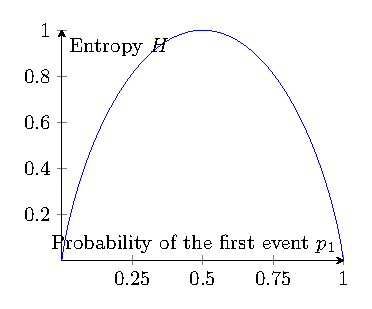
\includegraphics[width=0.55\linewidth,height=\textheight,keepaspectratio,alt={Entropy curve peaking when two outcomes each have probability one half.}]{chapters/../assets/figures/chapter05/fig-info-h.pdf}

}

\caption{\label{fig-info-h}Shannon entropy of two mutually exclusive
events.}

\end{figure}%

Figure~\ref{fig-info-h} shows that the entropy function is smooth with
regard to changes in the probability \(p_1\). When the two mutually
exclusive events are equally likely \(p_1=p_2=0.5\), the entropy of the
system is at its maximum (the peak in the middle).

It has been proved that, with any number of mutually exclusive events,
the greatest entropy is achieved when all events are equally possible.
Imagine a number of applicants compete for the same position. When
everyone has an equal chance and there is no leading candidate, it is
the most uncertain situation with the greatest entropy.

\begin{figure}

\centering{

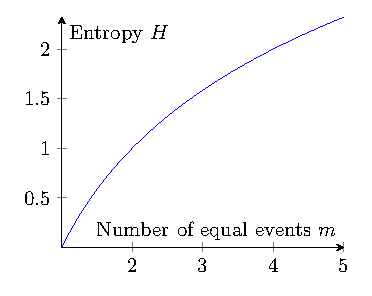
\includegraphics[width=0.55\linewidth,height=\textheight,keepaspectratio,alt={Increasing logarithmic curve showing entropy as the number of equally likely outcomes grows.}]{chapters/../assets/figures/chapter05/fig-info-h-m.pdf}

}

\caption{\label{fig-info-h-m}Shannon entropy of \(m\) equally likely
events.}

\end{figure}%

Figure~\ref{fig-info-h-m} plots entropy \(H\) vs.~the number of equally
likely events \(m\). When the number of events (choices) increases, so
does the entropy. With an increasingly larger pool of applicants for a
position -- supposedly with equal chances -- the harder it is to predict
who will be hired in the end.

A third property of the Shannon entropy is related to how the entropy of
one system can be computed based on entropies of its sub-systems. Let us
look at a simple example: Three candidates running for office, with
candidate \(1\) from party \(A\) and candidates \(2\) and \(3\) from
party \(B\). Suppose their probabilities of winning the election are
estimated as follow:

\[\begin{aligned}
  p_1 & = & 0.3 \\
  p_2 & = & 0.2 \\
  p_3 & = & 0.5
\end{aligned}\]

We can easily compute the overall entropy by:

\[\begin{aligned}
  H_{overall}
  & = & -0.3 \log_2 0.3 - 0.2 \log_2 0.2 - 0.5 \log_2 0.5 \\
  & = & 1.485
\end{aligned}\]

We can also look at the sub-systems, i.e.~parties \(A\) and \(B\), and
their entropies. The probability of party \(A\) is the same as that of
candidate \(1\), \(p_A = p_1 = 0.3\), whereas the probability of party
\(B\) is the sum of its candidates' probabilities
\(p_B = 0.2 + 0.5 = 0.7\). Therefore, the two-party system has an
entropy of:

\[\begin{aligned}
  H_{AB}
  & = & -0.3 \log_2 0.3 - 0.7 \log_2 0.7 \\
  & = & 0.881
\end{aligned}\]

Party \(A\) only has one candidate, which has a \(100\%\) chance to
"win" within the party, and there is no uncertainty:

\[\begin{aligned}
  H_A
  & = & - 1 \times \log_2 1 \\
  & = & 0
\end{aligned}\]

Of party \(B\), there are two candidates with overall probabilities
\(p_2 = 0.2\) and \(p_3=0.5\), which can be translated into the
following probabilities \emph{within} the party:

\[\begin{aligned}
  p_{B2} & = & \frac{0.2}{0.2+0.5} \\
      & = & \frac{2}{7} \\
  p_{B3} & = & \frac{0.2}{0.2+0.5} \\
      & = & \frac{5}{7}
\end{aligned}\]

Therefore, the sub-system entropy of party \(B\) is:

\[\begin{aligned}
  H_B
  & = & - \frac{2}{7} \log_2 \frac{2}{7} - \frac{5}{7} \log_2 \frac{5}{7} \\
  & = & 0.863
\end{aligned}\]

In the end, the entropy of the entire system overall can be computed by
the weighted sum of its sub-systems:

\[\begin{aligned}
  H_{overall}
  & = & H_{AB} + p_A H_A + p_B H_B \\
  & = & 0.881 + 0.3 \times 0 + 0.7 \times 0.863 \\
  & = & 1.485
\end{aligned}\]

This is exactly what we got in
Equation~\hyperref[eq-info-h_overall]{{[}eq-info-h\_overall{]}}, where
we looked at the overall of three candidates regardless of their parties
(sub-systems). It can be shown that the overall entropy of any
probability distribution is the same as the weighted sum of entropies of
its sub-systems.

\subsection{Entropy in Thermodynamics?}\label{entropy-in-thermodynamics}

The notion of \emph{entropy} predated Shannon's information theory, and
had been used in thermodynamics and statistical mechanics. Historically
the information-theoretic entropy has been taken as a completely
separated development and is only mathematically analogous to the same
notion in thermodynamics. Many regarded the identical name as an
accident.\footnote{According to one story, John von Neumann advised
  Shannon to use the term \emph{entropy} for two reasons: first because
  it is something already used in statistical mechanics, and second, "as
  nobody knows what entropy is, whenever you use the term you will
  always be at an advantage."}

Nonetheless, several prominent theoretical physicists, including the
late John A. Wheeler, have argued that the two are equivalent if given
the same dimensionality.(Bekenstein 2003) While it is tempting to
elaborate on the debate, for now we shall avoid the unsettled issues but
emphasize a few useful points drawn from statistical mechanics.

In thermodynamics, entropy measures the degree of uncertainty in the
distribution of microscopic states, e.g.~the distribution of temperature
in a body of gas. This uncertainty, sometimes referred to as some
\emph{disorder} -- not of the system itself, but according to the human
"eye" -- can be attributed to the lack of information or knowledge about
the states.

The second law of thermodynamics asserts that the \emph{entropy} of a
closed system, without external energy input, will never decrease. That
is, it requires energy to reduce entropy and restore \emph{order}. While
the thought experiment of \emph{Maxwell's demon} appears to suggest that
this second law can be violated, some physicists had resorted to the
notion of \emph{information} in refuting the paradox between energy and
entropy.\footnote{The Maxwell's demon goes like this: If we place a
  demon at the gate between two chambers of gas and it only allows
  active particles to pass the gate in one direction, then the overall
  entropy of the two chambers as one closed system will decrease}. One
can argue that obtaining information (e.g.~about "active" particles)
requires energy and the outcome of Maxwell's demon does not violate the
second law of thermodynamics. In this reasoning, there appears to be
some form of connection between information and entropy even in the
physical reality of thermodynamics.

In statistical mechanics, entropy is a measure of uncertainty given the
potential number of arrangements or configurations. For example, thermal
entropy of gas is due to the lack of knowledge about its particle
positions and velocities. It is a macroscopic measure of probability
distributions on related microscopic states. Mathematically, this is
consistent with quantifying entropy in the arrangements of coding and
communication given a probability distribution.

\subsection{Applications}\label{applications}

Shannon's mathematical theory of communication, commonly known as the
information theory, has been used in a wide spectrum of areas including
digital coding, communication, and information technology applications.

On binary media such as digital computer systems, for example, Shannon
entropy offers the basic unit of \emph{bit} to quantify the amount of
information and the necessary space to store and process it. It also
enables a fundamental paradigm shift in the study of communication
channel capacity, from signal power (energy) to bandwidth (frequency).

Modeling information as reduction of entropy (uncertainty) provides a
valuable vehicle in the design and engineering of digital information
systems. In information retrieval and text mining, for example,
information and probability theories have provided important guidance to
the development of classic methods for representation, ranking, and
classification.(Robertson and Zaragoza 2009) For example, computing
information amounts of words based on their probability distributions
enables the weighing and ranking of terms for text representation.

Let's look at the following example where entropy offers a powerful
evaluation tool --

Data mining algorithms often require certain evaluations conducted and
decisions made during related training or modeling processes. For
example, decision tree construction needs a method to evaluate how good
a tree branch is given its membership composition. Data clustering aims
to put like entities together and one needs to measure how similar or
dissimilar entities are within each cluster. In any of these
applications, a good metric of internal homogeneity or heterogeneity
(within each decision tree branch or cluster) is critical for the
success of related processes.

Suppose we are to group a set of shapes (of types \(\triangle\),
\(\heartsuit\), \(\bigcirc\)) into related clusters or branches, and
Table~\hyperref[tab-info-groups]{1.2} shows four clusters with different
membership compositions.

\protect\phantomsection\label{tab-info-groups}
\begin{longtable}[]{@{}
  >{\raggedright\arraybackslash}p{(\linewidth - 22\tabcolsep) * \real{0.0833}}
  >{\raggedright\arraybackslash}p{(\linewidth - 22\tabcolsep) * \real{0.0833}}
  >{\raggedright\arraybackslash}p{(\linewidth - 22\tabcolsep) * \real{0.0833}}
  >{\raggedright\arraybackslash}p{(\linewidth - 22\tabcolsep) * \real{0.0833}}
  >{\raggedright\arraybackslash}p{(\linewidth - 22\tabcolsep) * \real{0.0778}}
  >{\raggedright\arraybackslash}p{(\linewidth - 22\tabcolsep) * \real{0.0833}}
  >{\raggedright\arraybackslash}p{(\linewidth - 22\tabcolsep) * \real{0.0778}}
  >{\raggedright\arraybackslash}p{(\linewidth - 22\tabcolsep) * \real{0.0778}}
  >{\raggedright\arraybackslash}p{(\linewidth - 22\tabcolsep) * \real{0.0778}}
  >{\raggedright\arraybackslash}p{(\linewidth - 22\tabcolsep) * \real{0.0722}}
  >{\raggedright\arraybackslash}p{(\linewidth - 22\tabcolsep) * \real{0.0722}}
  >{\raggedright\arraybackslash}p{(\linewidth - 22\tabcolsep) * \real{0.0722}}@{}}
\caption{Four clusters of shapes}\tabularnewline
\toprule\noalign{}
\endfirsthead
\endhead
\bottomrule\noalign{}
\endlastfoot
\(\triangle\) & \(\triangle\) & \(\triangle\) & \(\triangle\) &
\(\triangle\) & \(\heartsuit\) & \(\triangle\) & \(\triangle\) &
\(\triangle\) & \(\bigcirc\) & \(\bigcirc\) & \(\bigcirc\) \\
\(\heartsuit\) & \(\heartsuit\) & \(\heartsuit\) & \(\heartsuit\) &
\(\bigcirc\) & \(\bigcirc\) & \(\triangle\) & \(\bigcirc\) &
\(\bigcirc\) & \(\bigcirc\) & \(\bigcirc\) & \(\bigcirc\) \\
\(\bigcirc\) & \(\bigcirc\) & \(\bigcirc\) & \(\bigcirc\) & \(\bigcirc\)
& \(\bigcirc\) & \(\bigcirc\) & \(\bigcirc\) & \(\bigcirc\) &
\(\bigcirc\) & \(\bigcirc\) & \(\bigcirc\) \\
\multicolumn{3}{@{}>{\raggedright\arraybackslash}p{(\linewidth - 22\tabcolsep) * \real{0.2500} + 4\tabcolsep}}{%
(1)} &
\multicolumn{3}{>{\raggedright\arraybackslash}p{(\linewidth - 22\tabcolsep) * \real{0.2444} + 4\tabcolsep}}{%
(2)} &
\multicolumn{3}{>{\raggedright\arraybackslash}p{(\linewidth - 22\tabcolsep) * \real{0.2333} + 4\tabcolsep}}{%
(3)} &
\multicolumn{3}{>{\raggedright\arraybackslash}p{(\linewidth - 22\tabcolsep) * \real{0.2167} + 4\tabcolsep}@{}}{%
(4)} \\
\end{longtable}

One classic metric is \emph{purity}, which measures the size of the
dominant type (class) relative to the entire cluster. That is:

\[\begin{aligned}
  Purity(c) & = & \frac{1}{n_c} \max_t c_t
\end{aligned}\]

where \(n_c\) is the size of cluster \(c\) (the total number of members)
and \(c_t\) is the number of members in \(c\) that belong to type \(t\).
For cluster (1) in Table~\hyperref[tab-info-groups]{1.2}, the members
are equally distributed among three types, each has \(3\) and the purity
is:

\[\begin{aligned}
  Purity(c_1)
  & = & \frac{1}{9} max(3, 3, 3) \\
  & = & \frac{3}{9}
\end{aligned}\]

For cluster (4), there is only one type, namely \(\bigcirc\), and its
purity is \(9/9 = 100\%\). So far, purity appears consistent with our
intuitive observation that cluster (4) is pure and cluster (1) is much
less so because it is consisted of three equal types.

If we apply purity to clusters (2) and (3) in
Table~\hyperref[tab-info-groups]{1.2}, we get:

\[\begin{aligned}
  Purity(c_2)
  & = & \frac{1}{9} max(2, 2, 5) \\
  & = & \frac{5}{9} \\
  Purity(c_3)
  & = & \frac{1}{9} max(4, 0, 5) \\
  & = & \frac{5}{9} \\
\end{aligned}\]

Both have the same purity score. However, it is clear that cluster (2)
has three types (2-2-5) and is more heterogeneous than cluster (3),
which only has two types (4-5). Because purity only relies on the
dominant type, it ignores the overall distribution and does not
differentiate between the two clusters here.

Now that we know Shannon entropy is a property of a probability
distribution, it can be applied to the problem here to measure member
distribution in the types. By converting the counts (frequencies) into
probabilities, we can compute the entropy of each cluster by:

\[\begin{aligned}
  H & = & - \sum_t p_t \log p_t
\end{aligned}\]

where \(p_t\) is the probability of type \(t\) and can be estimated by
\(c_t/n_c\), i.e.~the proportion of cluster \(c\) that is in type \(t\).
Hence:

\[\begin{aligned}
  H(c_1)
  & = & - 3 \times \frac{3}{9} \log \frac{3}{9} \\
  & = & 1.585 \\
  H(c_2)
  & = & - \frac{2}{9} \log \frac{2}{9} - \frac{2}{9} \log \frac{2}{9} - \frac{5}{9} \log \frac{5}{9}\\
  & = & 1.436 \\
  H(c_3)
  & = & - \frac{4}{9} \log \frac{4}{9} - \frac{5}{9} \log \frac{5}{9}\\
  & = & 0.991 \\
  H(c_4)
  & = & - \frac{9}{9} \log \frac{9}{9} \\
  & = & 0
\end{aligned}\]

From clusters (1) through (4), the entropy decreases. Cluster (1) has an
even distribution among the three types and the most heterogeneous with
greatest entropy (disorder). Cluster (4), on the other hand, is the
ideal and purest with \(0\) entropy. Furthermore, cluster (3) is not as
broadly distributed as cluster (2) and has less entropy. In terms of the
examples in Table~\hyperref[tab-info-groups]{1.2}, Shannon entropy
measures the overall distribution better than purity.

\section{Limits and Other Measures}\label{limits-and-other-measures}

Despite its broad use, there are assumptions that define the boundary of
the classic information theory, beyond which its application requires
careful examination of the domain context. For one, the basic assumption
that information entails the reduction of entropy does not always hold
true. There are abundant examples where having more information may lead
to confusion and increased uncertainty. Sometimes, less is more.

The original purpose of Shannon's theory, as noted in his master piece,
was for engineering communication systems where the ``meaning of
information was considered irrelevant''. It is about technical problems
that can be treated as independent the semantic content of
messages.(RAPOPORT 1953)

Shannon entropy is best used in applications where uncertainty or the
amount of (missing) information is indeed a \emph{property} of a
distribution, no less and no more. In domains where receiving
information may lead to revised probabilities (change of beliefs) but
not necessarily reduction of uncertainty, Shannon entropy as a function
solely based on \emph{a} probability distribution becomes insufficient.

To clarify on this point, let us look at a real world example --

Consider the 2016 presidential election of the U.S.\footnote{While this
  is an example from politics, the analysis here is apolitical.} Poll
data and analytics had led many people to believe, up until the election
night, that Hillary Clinton would win a landslide against Donald Trump.
A common prediction would put \(90\%\) for Clinton and \(10\%\) for
Trump\footnote{The data are hypothetical, rough estimates of the
  election day sentiment. For a simplified discussion, we only focus on
  candidates of the two major parties rather than the actual four.},
resulting in an entropy of:

\[\begin{aligned}
  H_{2016}
  & = & - 0.9 \log 0.9 - 0.1 \log 0.1 \\
  & = & 0.469
\end{aligned}\]

which is much less than the entropy of a 50-50 case (\(H=1\)). So with
this belief, there was very little uncertainty (doubt) about the outcome
given one was highly favored (likely) to win.

In terms of Shannon entropy, there was \emph{little} missing information
in that belief (probability distribution). This would make sense if the
likely candidate eventually won.

However, when the election turned out in the opposite direction, many
would immediately ask questions like "what went wrong" and "what did the
polls miss?" Clearly there was in fact lots of missing information in
the polls. And the surprising result does require tremendous amount of
explanation (with additional information).

But the Shannon entropy does not "care" as it only models the estimated
distribution, regardless of the outcome or what turns out to be correct.

We can draw from the above example that different amounts of information
are needed to explain different (and sometimes opposite) outcomes. The
amount of information should depend not only on the uncertainty of
inferences but also on the ultimate outcome (the correct inference or
the true probability distribution).

We reason that while uncertainty is a property of a specified
probability distribution, the amount of information required to explain
the outcome and more generally to explain a probability distribution
change is more complex than a linear function of uncertainty and should
depend on both distributions, i.e.~a belief and a changed belief. We
will discuss a couple of models that account for this relative entropy
change.

\subsection{Relative Entropy}\label{relative-entropy}

Relative Entropy, or KL Divergence, models the amount of information it
loses when one uses certain \emph{estimates} to approximate a true
probability distribution.(Kullback and Leibler 1951)

Given a probability distribution \(P\) and an estimated distribution
\(Q\) of the same variable, the relative entropy, or information loss
due to the estimation, can be computed by:

\[\begin{aligned}
  KL(P||Q)
  & = & (- \sum_i p_i \log q_i) - (- \sum_i p_i \log p_i) \\
  & = & \sum_i p_i \log \frac{p_i}{q_i}
\end{aligned}\]

where \(p_i\) and \(q_i\) are, respectively, the (true) probability and
estimate of the \(i^{th}\) inferences. As shown in the formula, the KL
divergence measures the difference in the number of arrangements between
\(Q\) and \(P\), weighted by the \emph{true} probabilities in \(P\).
This is the amount of information (in \emph{bits} with log base \(2\))
lost in the estimates.

We apply this to the 2016 election example. Let \(Q\) denote the
estimates according to polls: \(q_{clinton}=0.9\) and
\(q_{clinton}=0.1\). \(P\) denotes the true probabilities (actual
result).

Suppose the election went as predicted, i.e.~with a Clinton win
\(p_{clinton}=1\). KL can be computed by:

\[\begin{aligned}
  KL(P_{clinton}||Q)
  & = & 1 \times \log \frac{1}{0.9} + 0 \times \log \frac{0}{0.1} \\
  & = & 0.152
\end{aligned}\]

Now that the election actually turned out the opposite, i.e.~with a
Trump win \(p_{trump}=1\), KL is in fact:

\[\begin{aligned}
  KL(P_{trump}||Q)
  & = & 0 \times \log \frac{0}{0.9} + 1 \times \log \frac{1}{0.1} \\
  & = & 3.322
\end{aligned}\]

which indicates a much greater (about \(20\) times) information loss,
compared to the \emph{true} distribution (outcome), in the estimated
chances based on poll data. The relative entropy does appear to capture
the \emph{surprise} factor.

KL divergence has a few useful properties. KL is non-negative for any
distributions. It increases with increasing differences in the \(P\) and
\(Q\) values and can approach infinity with an infinite
\(\frac{p_i}{q_i}\) ratio, e.g.~with a \(q_i \to 0\) -- that is, when
something is mistakenly believed to be impossible when it is in fact
possible.

KL divergence cannot, however, be referred to as a distance measure or
metric. To qualify as a metric distance, a function has to satisfy the
following conditions: 1) it is non-negative, 2) it returns zero for two
identical sets of values, 3) it is symmetric, and 4) it satisfies the
triangular inequality.

KL does meet the first two requirements on non-negativity and identify
of indiscernibles -- KL is zero, \(KL(P||Q)=KL(Q||P)=0\), only when the
two distributions are identical -- but does not satisfy the triangular
inequality.

For any distance function \(d\), the triangle inequality requires that,
given three points (sets of values or probability distributions) \(A\),
\(B\), and \(C\), the sum of two distances (sides) is no less than the
third. This can be illustrated in Figure~\ref{fig-info-triangle}, where
any two distances (sides) \(d(A,B) + d(B,C) \ge d(A,C)\).

\begin{figure}

\centering{

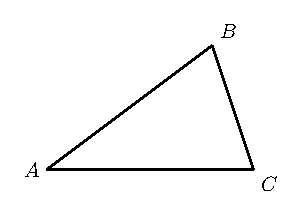
\includegraphics[width=0.5\linewidth,height=\textheight,keepaspectratio,alt={Triangle with vertices A, B, and C and labeled distances between them.}]{chapters/../assets/figures/chapter05/fig-info-triangle.pdf}

}

\caption{\label{fig-info-triangle}Triangle inequality: the sum of two
distances is never less than the third, \(d(A,B) + d(B,C) \ge d(A,C)\).}

\end{figure}%

KL divergence does not satisfy the triangle inequality. That is, it does
allow \(KL(A||B) + KL(B||C) < KL(A||C)\) to happen under certain
conditions. In addition, KL is not symmetric and the divergence from
\(Q\) to \(P\) is not the same as that from \(P\) to \(Q\), i.e.
\(KL(P||Q) \ne KL(Q||P)\), where \(P\) and \(Q\) are not identical.

KL divergence extends the classic Shannon entropy and offers an
alternative to measuring information as a linear reduction of entropy.
However, the fact that it is not symmetric and not a metric disqualifies
it from certain applications where a geometric distance is fitting.

One important consequence of not being a metric is that one cannot add
up the amounts of divergence in the \emph{course} of probability
changes. It is meaningless to add \(KL(A||B)\) and \(KL(B||C)\), which
has little to do with \(KL(A||C)\). In other words, one cannot discuss
the sum of information in KL terms. In addition, as discussed earlier,
KL divergence can approach infinity and there is no upper bound.

KL divergence has enabled important development in statistical analysis.
Mutual information, for example, is the KL relative entropy between the
joint distribution of two random variables and the product of their
marginal distributions.

In information retrieval and text mining, the classic IDF (inverse
document frequency) term weighting scheme in can be regarded as a
function derived from KL divergence. Later in the chapter, we will
discuss related problems due to undesirable properties of KL and a
remedy developed and tested recently.

\section{Jensen-Shannon Divergence}\label{jensen-shannon-divergence}

One approach to make KL divergence symmetric is to compute the sum of
its scores in both ways. For example:

\[\begin{aligned}
  J(P, Q) & = & KL(P||Q) + KL(Q||P)
\end{aligned}\]

However, this does not resolve the problem of no upper bound; nor does
it satisfy other desirable properties such as triangle inequality.
Another alternative is the Jensen-Shannon divergence, which measures the
average of information losses using the mixture of two probability
distributions:

\[\begin{aligned}
  JS(P||Q) & = & \frac{KL(P||M) + KL(Q||M)}{2}
\end{aligned}\]

where \(M\) is the mixture probability, i.e.~\(M=\frac{P+Q}{2}\). It is
easy to show that \(JS(P||Q)=JS(Q||P)\).

A metric can be derived by taking the square root of Jesen-Shannon
divergence:

\[\begin{aligned}
  JSR(P||Q) & = & \sqrt{\frac{KL(P||M) + KL(Q||M)}{2}}
\end{aligned}\]

Using the discussed 2016 election, for example, JSR can be computed for
a Trump win, i.e.~\(P_{trump}=1\) and \(P_{clinton}=0\). Given polling
data shows chances before election night, \(Q_{trump}=0.1\) and
\(Q_{clinton}=0.9\), the mixture probability distribution \(M\) is:

\[\begin{aligned}
  M_{trump} & = & \frac{1+0.1}{2} \\
            & = & 0.55 \\
  M_{clinton} & = & \frac{0+0.9}{2} \\
            & = & 0.45
\end{aligned}\]

The Jesen-Shannon divergence is:

\[\begin{aligned}
  JS(P||Q)
  & = & \frac{KL(P||M) + KL(Q||M)}{2} \\
  & = & \frac{1\times\log\frac{1}{0.55} + 0\times\log\frac{0}{0.45} + 0.1\times\log\frac{0.1}{0.55} + 0.9\times\log\frac{0.9}{0.45}}{2} \\
  & = & 0.758
\end{aligned}\]

Then JSR is the square root of JS:

\[\begin{aligned}
  JSR(P||Q)
  & = & \sqrt{0.758} \\
  & = & 0.871
\end{aligned}\]

In the evening of the election, data and the outcome of some states led
to an increased likelihood of a Trump win. Suppose the changed
probability estimates became \(Q'\) where \(Q'_{trump}=0.9\) and
\(Q'_{clinton}=0.1\), the opposite of the earlier estimates \(Q\).

We can compute JSR between \(Q\) and \(Q'\):

\[\begin{aligned}
  JSR(Q'||Q)
  & = & \frac{0.9\times\log\frac{0.9}{0.5} + 0.1\times\log\frac{0.1}{0.5} + 0.1\times\log\frac{0.1}{0.5} + 0.9\times\log\frac{0.9}{0.5}}{2} \\
  & = & 0.729
\end{aligned}\]

We can also compute JSR between \(Q'\) and \(P\):

\[\begin{aligned}
  JS(P||Q')
  & = & \frac{1\times\log\frac{1}{0.95} + 0\times\log\frac{0}{0.05} + 0.9\times\log\frac{0.9}{0.95} + 0.1\times\log\frac{0.1}{0.05}}{2} \\
  & = & 0.228
\end{aligned}\]

Clearly, the sum of \(JS(P||Q')\) and \(JSR(Q'||Q)\) is
\(0.228 + 0.729 = 0.957\), which is greater than \(JS(P||Q)=0.871\).
This does not violate the triangular inequality.

It has been shown that the square root of Jesen-Shannon divergence (JSR)
satisfies triangular inequality.(Endres and Schindelin 2006) And because
JS measures the average information loss to the mixture probability, the
amount is the same for \(JS(P||Q)\) and \(JS(Q||P)\) -- that is, JS is a
symmetric function and so is its square root JSR.

JSR does satisfy all the requirements for a distance function and can be
used where related metric properties are desired. Whereas JS divergence
can still be regarded as measuring the amount of information in bits (at
least with log base \(2\)), it is not clear what its square root (JSR)
actually means.

\section{IDF and KL Divergence}\label{idf-and-kl-divergence}

Before we get to an alternative to the divergence measures, we shall
discuss an important connection between the classic IDF (inverse
document frequency) method for text processing and KL divergence. The
theoretical connection will enable us to see why certain treatments
based on IDF may or may not be a good idea.

As we discussed in chapter~, one important step in text processing is to
determine how informative each term is and how much weight should be
given. To do this, let's look at probabilities associated with a term.

Suppose we randomly draw a document from a collection of \(N\)
documents, the likelihood of observing term \(t\) in the document can be
estimated by:

\[\begin{aligned}
  Q(t) & = & \frac{n_t}{N}
\end{aligned}\]

where \(n_t\) is the number of documents containing term \(t\). Its
complementary probability, i.e.~the probability that term \(t\) does not
occur, can be computed by \(\bar{Q}(t) = \frac{N - n_t}{N}\).

Now with a specific document where term \(t\) actually appears, its
probability is \(P(t)=1\) and the complementary \(\bar{P}(t)=0\). We can
compute the amount of information loss due to the probability estimate
\(Q\) using KL divergence:

\[\begin{aligned}
  KL(P||Q)
  & = & P(t) \log \frac{P(t)}{Q(t)} + \bar{P}(t) \log \frac{\bar{P}(t)}{\bar{Q}(t)} \\
  & = & 1 \log \frac{1}{\frac{n_t}{N}} + 0 \log \frac{0}{\frac{N - n_t}{N}} \\
  & = & \log \frac{N}{n_t}
\end{aligned}\]

which is exactly the IDF (inverse document frequency) term weighting
scheme, where \(n_t\) is document frequency (DF).

Here we see that the classic IDF can be regarded as an application of KL
divergence in the text processing context. In related applications, it
is common to compute the sum of IDF weights for processes such as
document ranking (in information retrieval). However, this might not be
the proper treatment for a non-metric.

As we observed earlier, KL divergence does not have an upper bound and
can reach infinity. In particular, IDF as an information amount of a
term can be extremely large when the term is very rare. When term IDF
weights are combined to determine ranking, for example, the rare term
will dominate the ranking score and the weights of other terms will no
longer matter.

\section{Least Information Theory (LIT)}\label{ch-info-lit}

The Least Information Theory (LIT), a very recent development, has
attempted to resolve the problems associated with divergence-related
information measures.(Ke 2015) In particular, its major objective is to
create an information quantity that: 1) is a metric, 2) can be
interpreted properly such as in terms of bits, and 3) has an upper bound
and does not produce infinite values even with extreme probabilities.

Based on Shannon entropy, LIT does not assume a linear relation between
information and the reduction of entropy. Rather, we acknowledge that
receiving information can lead to either an increase or decrease of
entropy, and measures the amount of information as the sum of
microscopic, absolute entropy changes. Given two probability
distributions \(P\) and \(Q\) on \(m\) discrete inferences of the same
variable, their Shannon entropies can be computed by:

\[\begin{aligned}
  H(P) & = & - \sum_{i=1}^{m} p_i \log p_i \\
  H(Q) & = & - \sum_{i=1}^{m} q_i \log q_i
\end{aligned}\]

Let \(dH_i\) be the amount of entropy change due to a very small change
in the probability of the \(i^{th}\) inference \(dp_i\). We can compute
\(dH_i\) based on Shannon entropy:

\[\begin{aligned}
  dH_i & = & - \log p_i dp_i
\end{aligned}\]

This microscopic entropy represents the change of the weighted (\(p_i\))
number of arrangements (\(- \log p_i\) or \(\log \frac{1}{p_i}\)). It is
the change in the number of configurations due to a change weight
(probability). By integrating (aggregating) the microscopic changes, we
can compute the amount of entropy due to a greater, macroscopic
probability change from \(P\) to \(Q\) in the \(i^{th}\) inference:

\[\begin{aligned}
  I_i(P \to Q)
  & = & \int_{p_i}^{q_i} - \log p dp \\
  & = & \big| p_i (1-\ln p_i) - q_i (1-\ln q_i) \big|
\end{aligned}\]

The overall entropy change is the sum of entropy changes of all
inferences:

\[\begin{aligned}
  I(P \to Q)
  & = & \sum_{i=1}^{m} \big| p_i (1-\ln p_i) - q_i (1-\ln q_i) \big|
\end{aligned}\]

where \(m\) is the total number of mutually exclusive inferences,
i.e.~the number of discrete values of the probability distribution. Note
that in the final formula, the logarithm is always with a natural base
(\(\ln\)). This is the result of the integral of any log function.

The Least Information measure (LIT) in
Equation~\hyperref[eq-info-lit]{{[}eq-info-lit{]}} can be interpreted as
the minimum amount of information, in Shannon entropic terms,
\emph{necessary} for the probability distribution shift, or a change of
belief. In this model, information does not always reduce entropy -- in
fact, it can lead to entropy change in any direction. In addition, it
does not consider the removal of information, which can be regarded as
new information that refutes prior knowledge.

Figure~\ref{fig-info-lit} compares least information (LIT) with Shannon
entropy and KL divergence, using a binary example (of two mutually
exclusive inferences). The figure assumes the \(1^{st}\) inference to be
the ultimate outcome -- that is, it starts with a probability
distribution \(P\) (with some \(p_1\) and \(p_2\)) and ends with changed
distribution \(Q\), where \(q_1=1\) and \(q_2=0\). For example, the
reading of \((0.5, 1)\) on the LIT curve indicates the amount of least
information is \(1\) that changes the probability distribution from
\(P(0.5, 0.5)\) to \(Q(1, 0)\).

\begin{figure}

\centering{

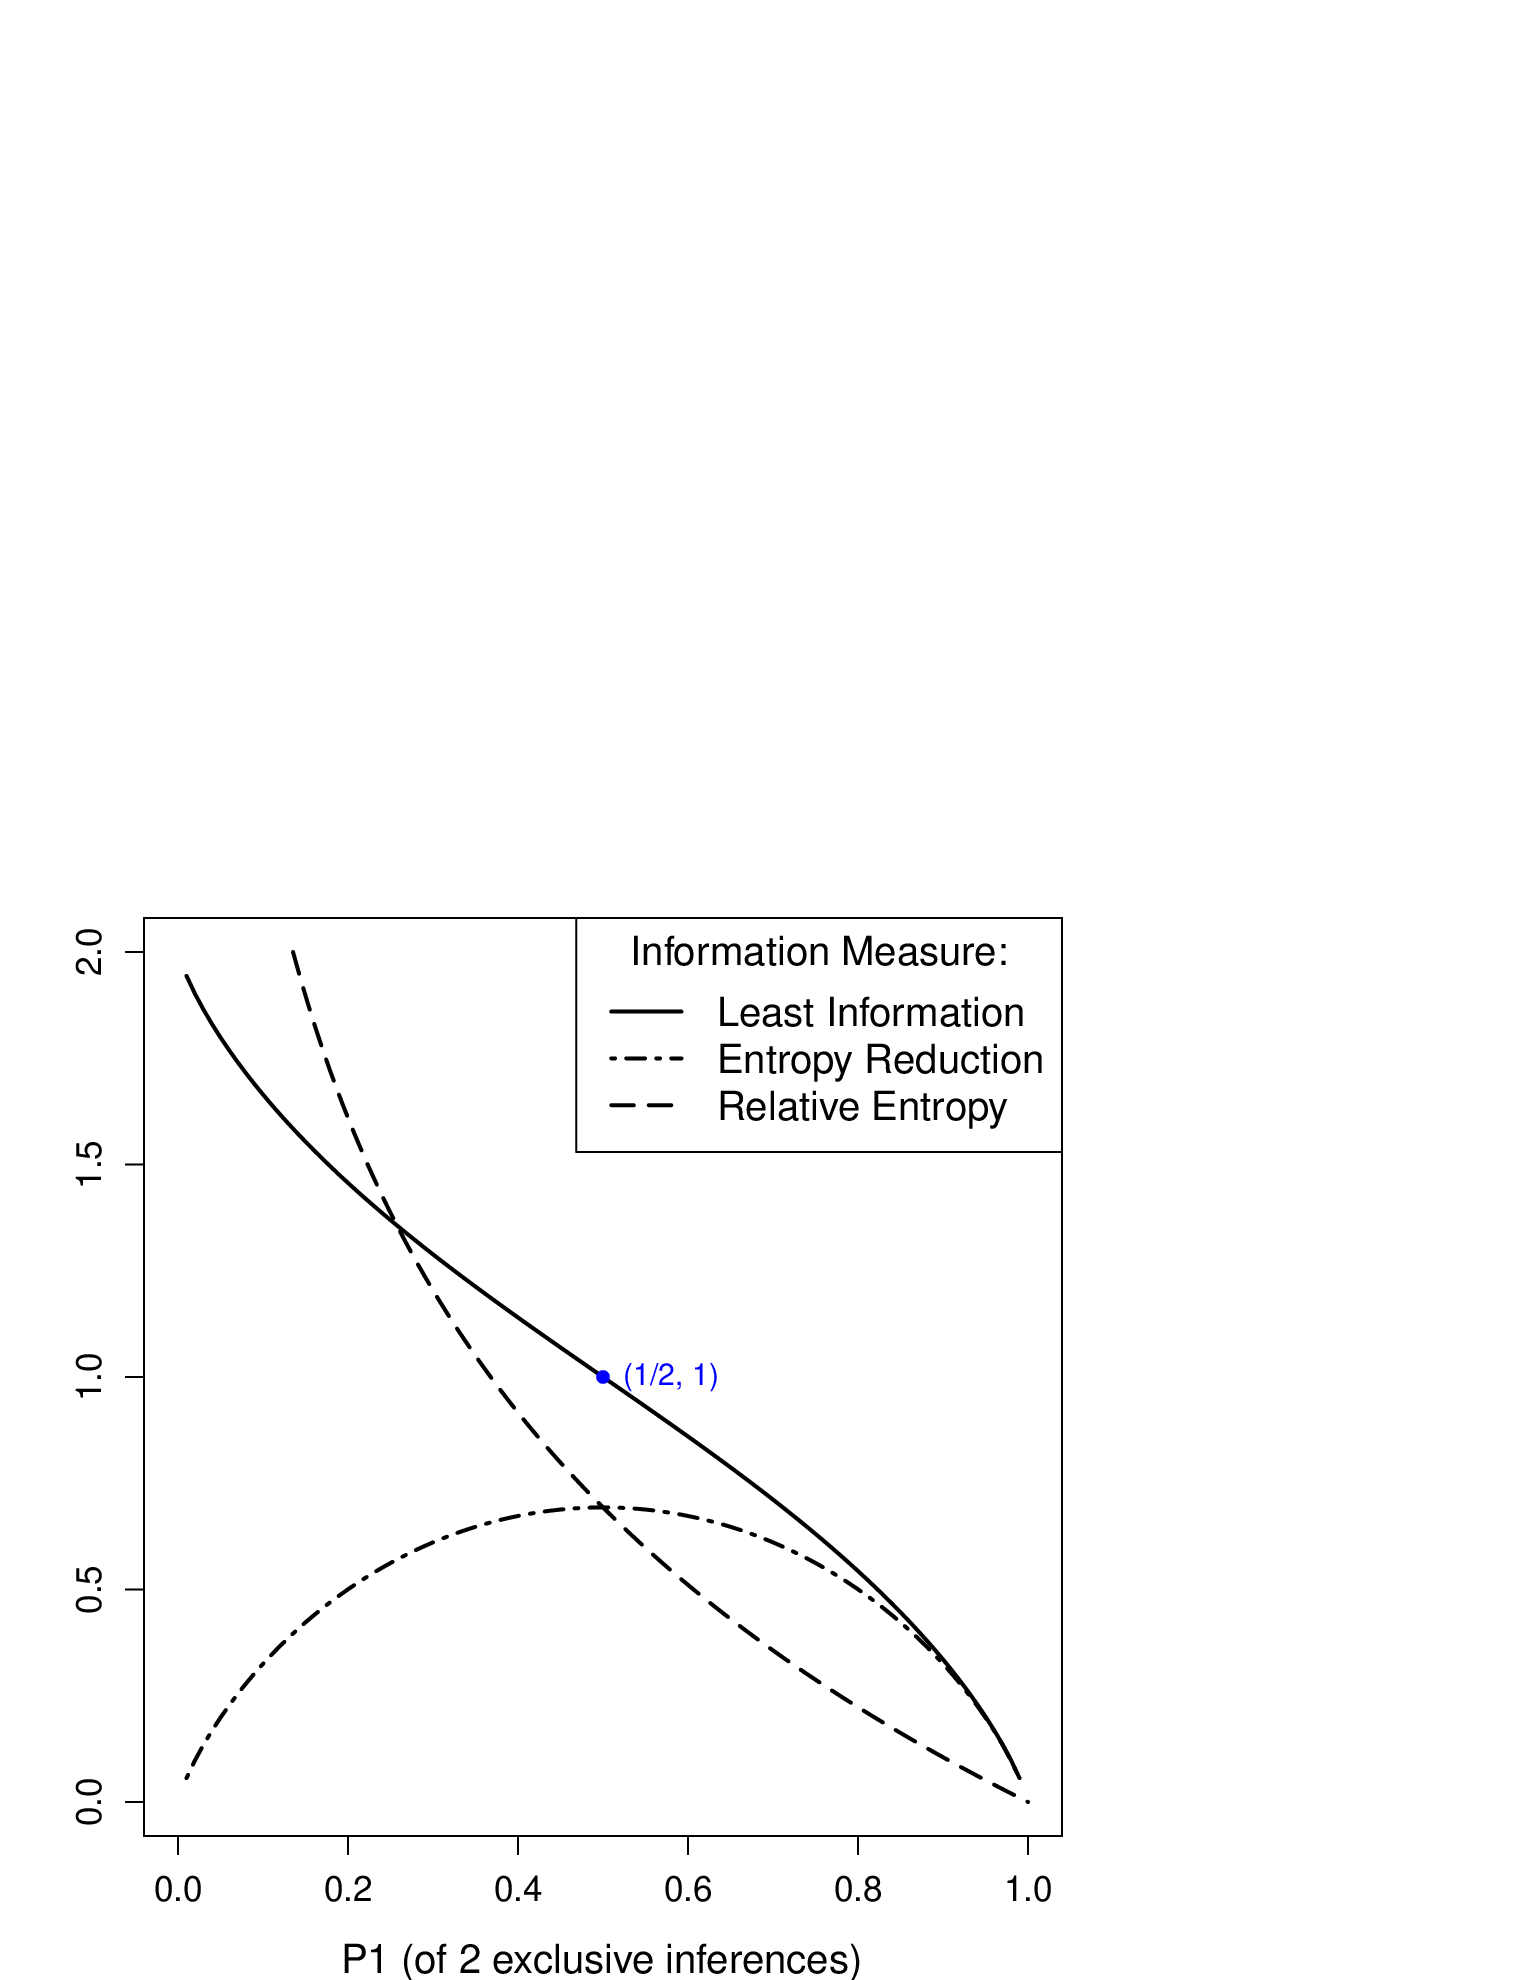
\includegraphics[width=2.5in,height=\textheight,keepaspectratio]{chapters/../assets/figures/info/lit.png}

}

\caption{\label{fig-info-lit}Least Information vs.~Shannon Entropy
vs.~KL Divergence. This shows the amount of information by reducing two
mutually exclusive inferences to certainty. The X axis is \(p_1\), the
probability of the \(1^{st}\) inferences. The Y axis is the amount of
information (I) in terms of each information measure. The \(1^{st}\)
inference is assumed to be the ultimate outcome (\(q_1=1\)) in the
figure.}

\end{figure}%

The symmetry of Shannon entropy indicates that the amount is the same
regardless of the outcome. KL divergence can approach infinity with
\(p_1 \to 0\). Least Information (LIT), however, is limited to the range
of \([0, 2]\) in the binary case.

Further examination of
Equation~\hyperref[eq-info-lit]{{[}eq-info-lit{]}} reveals that the
Least Information Theory (LIT) possesses several important properties:

\begin{enumerate}
\def\labelenumi{\arabic{enumi}.}
\item
  Non-negativity: \(I(P,Q) \ge 0\), the amount of least information is
  no less than zero.
\item
  Identity of indiscernibles: \(I(P,Q)=0\), if and only if \(P\) and
  \(Q\) are identical, i.e.~no change at all in the probability
  distribution.
\item
  Symmetry: \(I(P,Q)=I(Q,P)\), the amount of \emph{least information}
  required for a probability change from \(P\) to \(Q\) is the same as
  that from \(Q\) to \(P\).
\item
  Triangular inequality: \(I(P,Q) + I(Q,R) \ge I(P,R)\), among three
  probability distributions, the sum of two least information amount is
  no less than the third.
\item
  Addition of continuous change: \(I(P,Q) + I(Q,R) = I(P,R)\), when
  \(P \to Q\) and \(Q \to R\) are in the same direction of probability
  changes (i.e.~for each individual inference, they either both increase
  or both decrease its probability). In other words, amounts of
  \emph{least information} for small, continuous probability changes in
  the same directions add linearly to the amount responsible for the
  overall change.
\item
  Unit Information: In the special case when there are two equally
  possible inferences, the amount of \emph{least information} needed to
  explain/interpret an outcome (certainty) is one:
  \(I(p_1=p_2=\frac{1}{2} \to q_1 =1,q_2=0) = 1\) (see data point
  \((\frac{1}{2},1)\) in Figure~\ref{fig-info-lit}).
\item
  In the special case of reducing uncertain inferences to certainty (the
  ultimate case):

  \begin{itemize}
  \item
    With equally likely inferences, when there are more choices, the
    least information needed to explain an outcome is larger.
  \item
    The less likely the outcome, the larger the amount of \emph{least
    information} needed to explain it.
  \end{itemize}
\end{enumerate}

The first four properties listed above mean that the Least Information
(LIT) function is a distance metric. The \(5^{th}\) property can be
likened to a function such as euclidean distance, where small distances
in the same direction can add up to the overall distance. This is
illustrated in Figure~\ref{fig-info-dist-add}, where \(a+b=c\). This is
the only situation in which they are equal with the triangle inequality.

\begin{figure}

\centering{

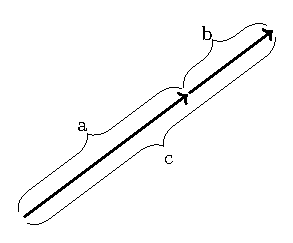
\includegraphics[width=0.55\linewidth,height=\textheight,keepaspectratio,alt={Three collinear points with adjacent distances a and b summing to total distance c.}]{chapters/../assets/figures/chapter05/fig-info-dist-add.pdf}

}

\caption{\label{fig-info-dist-add}Sum of distances in the same
direction, \(a+b=c\).}

\end{figure}%

We can test the Least Information Theory (LIT) on the example of 2016
election. Given the probability change from election day estimates of
\(Q_{trump}=0.1\) and \(Q_{clinton}=0.9\) to adjusted estimates of
\(Q'_{trump}=0.9\) and \(Q'_{clinton}=0.1\) to the final election
outcome of \(P_{trump}=1\) and \(Q_{clinton}=0\), one can compute the
the amounts of LIT on the two stages:

\[\begin{aligned}
  I(Q \to Q')
  & = & \big| 0.9 (1 - \ln 0.9) - 0.1 (1 - \ln 0.1) \big| \\
  &   & + \big| 0.1 (1 - \ln 0.1) - 0.9 (1 - \ln 0.9) \big| \\
  & = & 1.329 \\
  I(Q' \to P)
  & = & \big| 1 (1 - \ln 1) - 0.9 (1 - \ln 0.9) \big| \\
  &   &  + \big| 0 (1 - \ln 0) - 0.1 (1 - \ln 0.1) \big| \\
  & = & 0.335 \\
\end{aligned}\]

The overall LIT from early estimates \(Q\) to the final result \(P\) is:

\[\begin{aligned}
  I(Q \to P)
  & = & \big| 1 (1 - \ln 1) - 0.1 (1 - \ln 0.1) \big| \\
  &   & + \big| 0 (1 - \ln 0) - 0.9 (1 - \ln 0.9) \big| \\
  & = & 1.664 \\
  & = & 1.329 + 0.335
\end{aligned}\]

which is exactly the sum of the two stages' amounts, i.e.
\(I(Q \to P) = I(Q \to Q') + I(Q' \to P)\). This equality occurs because
\(Q \to Q'\) and \(Q' \to P\) represent probability changes in the same
directions -- that is, for each and every inference of the variable,
they either both increase or both decrease in that probability.

In the context of text processing and information retrieval, the least
information measure has produced superior results. Earlier we have shown
that the classic IDF (inverse document frequency) term weighting scheme
is a derived method from KL divergence. We can derive a similar method
based the least information. Again, the likelihood of having term \(t\)
in a random document from a text collection is \(Q(t)=\frac{n_t}{N}\),
where \(n_t\) is document frequency (DF)of term \(t\) and \(N\) the
total number of documents in the collection. The amount of least
information of actually observing term \(t\) in a specific document,
with \(P(t)=1\) and \(\bar{P}(t)=0\), can be computed by:

\[\begin{aligned}
  I(t)
  & = & I(Q_t, P_t) \\
  & = & \big| 1 (1 - \ln 1) - Q_t (1 - \ln Q_t) \big| \\
  &   & + \big| 0 (1 - \ln 0) - \bar{Q}_t (1 - \ln \bar{Q}_t) \big| \\
  & = & \underbrace{\big[ 1 - Q_t (1 - \ln Q_t) \big]}_{Q_t\ terms} + \big[ \bar{Q}_t ( 1 - \ln \bar{Q}_t) \big]
\end{aligned}\]

We may focus on the \(Q_t\) terms (the underbraced in
Equation~\hyperref[eq-info-lib2]{{[}eq-info-lib2{]}}) and neglect
\(\bar{Q}_t\) terms. We can define \(LIB(t,d)\), or least information
binary, to measure the informativeness of term \(t\) for document \(d\)
when it appears (\(t \in d\)) and when it does not (\(t \not \in d\)).
Given that \(Q_t = \frac{n_t}{N}\), we have:

\[
LIB(t,d) = \left\{
\begin{array}{l l}
  1 - \frac{n_t}{N} \Big(1 - \ln{\frac{n_t}{N}}\Big)    & t \in d \\
  - \frac{n_t}{N} \Big(1 - \ln \frac{n_t}{N}\Big)       & t \not\in d
\end{array}
\right.
\]

where \(n_t\) is the document frequency of term \(t\) and \(N\) is the
total number of documents. The larger the LIB, the more information the
term contributes to the document and should be weighted more heavily in
the document representation.

LIB is similar in spirit to IDF and its value represents the
discriminative power of the term when it appears in a document.
Nonetheless, LIB is formulated based on \emph{least information} of
query terms whereas IDF quantifies their KL divergence or the loss of
information due to estimates from the entire collection.

Research has shown that these methods derived from LIT worked extremely
well for text mining. In a range of experiments conducted on several
benchmark data sets, LIT-based methods outperformed their classic
counterparts such as TF*IDF in text clustering, classification, and
information retrieval.(Ke 2017)

\chapter{Data Preparation and Feature Engineering}\label{ch-preparation}

Trust, but verify.

\emph{Ronald Reagan}

\section{Data Quality and Provenance}\label{data-quality-and-provenance}

\section{Missing, Noisy, and Inconsistent
Data}\label{missing-noisy-and-inconsistent-data}

\section{Scaling, Normalization, and
Transformation}\label{scaling-normalization-and-transformation}

\section{Encoding Categorical and Structured
Variables}\label{encoding-categorical-and-structured-variables}

\section{Feature Selection and Dimensionality
Reduction}\label{feature-selection-and-dimensionality-reduction}

\section{Leakage and Reproducible
Pipelines}\label{leakage-and-reproducible-pipelines}

\section{Summary and Exercises}\label{summary-and-exercises}

There is no perfect data. In fact, a Kaggle 2017 survey showed that
\emph{dirty data} "is the most common problem for workers in the data
science realm."(Kaggle, n.d.) About 50\% of survey responses cited it as
a barrier at work.

\part{Learning from Data}

\chapter{Classification: From Neighbors to Neural
Networks}\label{ch-classification}

To be, or not to be,\\
that is the question...

\emph{Hamlet}, William Shakespeare

A binary question represents the basic decision making: yes or no, true
or false, etc. So how do we build a model to answer basic questions of
such? In particular, what does a model \emph{learn} from training data
to make predictions?

We shall continue to use a simple data set we encountered earlier,
namely the instances of shapes on the concept of \emph{standing}
vs.~\emph{lying}. Suppose we have identified \emph{width} and
\emph{height} as relevant attributes to the concept and
Table~\hyperref[tab-bin-shapes]{1.1} shows the data:

\protect\phantomsection\label{tab-bin-shapes}
\begin{longtable}[]{@{}cccl@{}}
\caption{Shapes data}\tabularnewline
\toprule\noalign{}
Width & Height & Standing? & \\
\midrule\noalign{}
\endfirsthead
\toprule\noalign{}
Width & Height & Standing? & \\
\midrule\noalign{}
\endhead
\bottomrule\noalign{}
\endlastfoot
4 & 2 & No & \\
5 & 9 & Yes & \\
9 & 5 & No & \\
2 & 4 & Yes & \\
1 & 8 & Yes & \\
5 & 3 & No & \\
\end{longtable}

\protect\phantomsection\label{tab-bin-shapes}{}

If the shape instances here can serve as training data, how can an
algorithm identify the relation between width and height as a predictor
for the concept of standing?

Given this simple problem -- simple to the human eye -- it may be
tempting to hardcode a selection structure such as \(height>width?\)
into an algorithm and make predictions without the training data. This,
however, defeats the purpose of data-driven machine learning. While we
can easily identify the classification rule with this small data set, it
is impossible to do so with massive data and more complex relations.

We should instead design a general strategy by which related rules and
relations can be captured from training data and then used in
predictions. What potential strategies can we propose? Let's look at a
few proposals.

\section{Lazy Learning}\label{lazy-learning}

The easiest approach to learning is not to learn at all, or simply
memorize all given materials without trying to understand them. We can
refer to this as \emph{lazy learning}, which is similar to what some
"lazy" students may do in reality.

But in the real world, how does a student perform on a test
(examination) if she has not understood anything at all? The solution is
to search, whether it is searching one's memory or materials and notes.
Without understanding, one will try to find notes and sections
\emph{most closely related} to a test question and develop an answer
based on the search result.

Likewise, in machine learning, a lazy learning method does not build any
\emph{model} at all but simply remembers (stores) training instances. To
predict on a test instance, the method searches its memory (training
data), finds the \emph{most closely related} instances to the test, and
predict the answer based on related instances it has found.

\subsection{K Nearest Neighbors (kNN)}\label{k-nearest-neighbors-knn}

We normally refer to the most closely related instances as the
\emph{nearest neighbors}.(Cover and Hart 1967) A classic lazy learning
algorithm is the \emph{k nearest neighbors} (kNN) approach, which makes
predictions based on \(k\) closest training instances.

But how does the algorithm find out which ones are the nearest? It needs
a function to measure the closeness or distance between two instances.
An example of such a distance function is the \emph{Euclidean distance},
which the length a straight line connecting the endpoints of two
instances \(u\) and \(v\) in dimensional space:

\[\begin{aligned}
  D(u,v) & = & \sqrt{\sum_{i=1}^{m} (u_i - v_i)^2}
\end{aligned}\]

where \(m\) is the number of dimensions (features) to represent each
data instance. Figure~\ref{fig-bin-ed} shows the shapes data on two
dimensions, i.e. \emph{width} and \emph{height}. Suppose a new instance
at \((4,7)\), i.e.~\(width=4\) and \(height=7\), is to be tested. The
dashed lines are the euclidean distances from the test instance to the
training instances.

\begin{figure}

\centering{

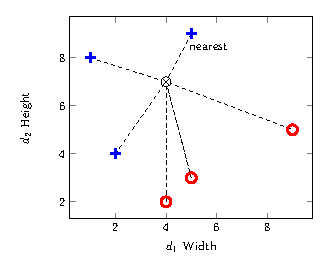
\includegraphics[width=0.7\linewidth,height=\textheight,keepaspectratio,alt={Nearest neighbors k=1, + denotes standing (positive) and denotes lying (negative). is the test instance.}]{chapters/../assets/figures/chapter07/fig-bin-ed.pdf}

}

\caption{\label{fig-bin-ed}Nearest neighbors \(k=1\), \(+\) denotes
\emph{standing} (positive) and \(\circ\) denotes \emph{lying}
(negative). \(\otimes\) is the test instance.}

\end{figure}%

If we set \(k=1\) for the kNN algorithm, we will use only \(1\) nearest
neighbor in prediction. The instance at \((5,9)\), which belongs to the
\emph{standing} class, has a distance from the test instance:

\[\begin{aligned}
  D[(4,7),(5,9)]
  & = & \sqrt{(4-5)^2 + (7-9)^2} \\
  & = & \sqrt{5}
\end{aligned}\]

This turns out to be the nearest in terms of Euclidean distance and the
test instance will be predicted \emph{standing} (positive) as well.

If we change \(k=3\), the \(3\) nearest neighbors will all be positive
(\(+\)) instances and the prediction for the above test instance will
remain positive.

For a different test instance, the \(k\) nearest neighbors might have
conflicting answers. For binary classification, one strategy is to pick
an odd number for \(k\) and let the nearest neighbors vote for the final
prediction.

\begin{figure}

\centering{

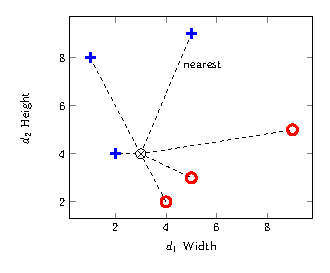
\includegraphics[width=0.7\linewidth,height=\textheight,keepaspectratio,alt={Nearest neighbors k=3, + denotes standing (positive) and denotes lying (negative). is the test instance.}]{chapters/../assets/figures/chapter07/fig-bin-ed2.pdf}

}

\caption{\label{fig-bin-ed2}Nearest neighbors \(k=3\), \(+\) denotes
\emph{standing} (positive) and \(\circ\) denotes \emph{lying}
(negative). \(\otimes\) is the test instance.}

\end{figure}%

Figure~\ref{fig-bin-ed2} shows another test instance at \((3,4)\). With
\(k=3\), it turns out that the three nearest neighbors include \(1\)
positive and \(2\) negatives. Using a majority vote strategy, the test
instance will be mistakenly classified into the negative (lying) class.

Two observations on the misclassification. First, the selection of \(k\)
does have an impact on the classification result. This is especially
true when training instances are sparse. With \(k=1\), the method relies
on one single instance for each test and is hardly robust. A larger
\(k\) can reduce the likelihood of predicting with atypical neighbors
but it introduces noise, e.g.~instances from across the class boundary
as illustrated in Figure~\ref{fig-bin-ed2}. Finding the optimal \(k\)
may require experimentation with data.

Second, more important, a lazy learner such as kNN does not have a
general function (model) to represent a concept of learning. It purely
relies on individual training instances for predictions and has \emph{no
generalizability}. Its success or failure depends on where the test
instance hit and how training data distribute around it. This is
analogous to a \emph{lazy} student who memorizes everything without
understanding -- she will not be able to answer a question for which no
similar examples have been provided in the materials.

\subsection{Other Distance Metrics}\label{other-distance-metrics}

Euclidean distance is a special case of a category of distance metrics
known as the \emph{Minkowski distance}, which is defined as:

\[\begin{aligned}
  MD(u, v) & = & \Big(\sum_{i=1}^{m} |u_i - v_i|^p\Big)^{1/p}
\end{aligned}\]

where \(p \ge 1\) and \(m\) is the number of dimensions. When \(p=2\),
this is the Euclidean distance. When \(p=1\), it becomes the Manhattan
distance:

\[\begin{aligned}
  MD_1(u, v) & = & \sum_{i=1}^{m} |u_i - v_i|
\end{aligned}\]

which is similar to counting the number of blocks in a city grid.

Another metric is similar to (but not exactly) Minkowski distance with
\(p=0\):

\[\begin{aligned}
  MD_0(u, v)
  & = & \sum_{i=1}^{m} (u_i - v_i)^0 \\
  & = & \sum_{u_i \ne v_i} 1
\end{aligned}\]

which counts the number of dimensions where there is a difference and is
often referred to as \emph{edit distance}. This is equivalent to
treating every dimension as a binary variable and the overall distance
is the amount of change in the bits.

\section{Linear Classifiers}\label{linear-classifiers}

As we observed, a lazy learner such as the k Nearest Neighbors (kNN)
does not actually \emph{learn} and build a model (function) that can be
generalized. Although kNN has decent performances in many applications,
it suffers in domains where, for example, test data appear on a
different scale from that of training data.

If we assume the classes can be separated by a \emph{function} (model)
with certain parameters, then building the model requires identification
of those parameters from training data. Surely there are way too many
different functional forms one can choose the model from. We start with
the simplest, a linear function.

With the shapes data in Figure~\ref{fig-bin-ed}, there are two variables
\(width\) (\(v_1\) for the \(x\) axis) and \(height\) (\(v_2\) for \(y\)
axis). \(y\) as a linear function of \(x\) can be written as
\(f(x) = a + b x\) or \(a + b x - y = 0\), with two parameters \(a\) and
\(b\) for two variables.

To make it extendable, We can rewrite this two-variable linear equation
as:

\[\begin{aligned}
  w_0 + w_1 v_1 + w_2 v_2 = 0
\end{aligned}\]

where the \(w\) parameters (instead of \(a\) and \(b\)) are to be
estimated. When there are more variables (dimensions), the function can
be extended to:

\[\begin{aligned}
  0
  & = & w_0 + w_1 v_1 + w_2 v_2 + ... + w_m v_m \\
  & = & w_0 + \sum_{i=1}^{m} w_i v_i
\end{aligned}\]

where \(m\) is the number of variables (dimensions).

With \(m=2\) for the shapes data, how do we estimate the parameters
\(w_0\), \(w_1\), and \(w_2\) in
Equation~\hyperref[eq-bin-lin2]{{[}eq-bin-lin2{]}} to linearly separate
the two classes \emph{standing} vs.~\emph{lying}? Note that a linear
equation in a 2-dimensional space is a straight line. It is a plane
(flat surface)) in a 3-dimensional space and a \emph{hyperplane} in a
higher-dimensional space.\footnote{A hyperplane in more three dimensions
  is hard to visualize. Mathematically, it shares the same functional
  form of Equation~\hyperref[eq-bin-lin]{{[}eq-bin-lin{]}} and is a
  natural extension of the lower-dimensional representation.} We will
discuss several approaches of the linear model.

\subsection{Between Centroids}\label{between-centroids}

We start with finding the \emph{centroid} for instances in each class. A
centroid is the center of the mass for a group of objects and can be
computed as the average of values on each dimension. The \(j^{th}\)
dimension of the centroid for class \(c\) is computed by:

\[\begin{aligned}
  \mu_{j}(c) & = & \frac{\sum_{i=1}^{n_c} v_{ij}}{n_c}
\end{aligned}\]

where \(v_{ij}\) is the value of the \(j^{th}\) dimension of the
\(i^{th}\) instance in class \(c\). Following this equation, the
centroids for the positive (standing) and negative (lying) classes can
be obtained:

\[\begin{aligned}
  \mu(\oplus)
  & = & \big( \mu_1(\oplus), \mu_2(\oplus) \big) \\
  & = & \big( \frac{5+2+1}{3}, \frac{9+4+8}{3} \big) \\
  & = & \big( \frac{8}{3}, 7 \big) \\
  \mu(\ominus)
  & = & \big( \frac{4+5+9}{3}, \frac{2+3+5}{3} \big) \\
  & = & \big( 6, \frac{10}{3} \big)
\end{aligned}\]

Figure~\ref{fig-bin-lin_cent} shows the two centroids and a dashed line
with an arrowhead connecting them. The arrow represents a vector in the
direction
\(\vec{\mu} = (6-\frac{8}{3}, \frac{10}{3} - 7) = (\frac{10}{3}, - \frac{11}{3})\),
whereas the middle of the dashed line is
\(\bar{\mu} = (\frac{13}{3}, \frac{31}{6})\).

Now if we can find a linear equation, i.e.~another straight line, that:
1) passes through the middle of the dashed line (equal to each
centroid), and 2) is perpendicular to the dashed line, then any point on
the linear equation (line) should have an equal distance from both
centroid. In this case, the line can serve as the \emph{boundary}
between the two classes.

Now, identifying the linear equation turns out to be very
straightforward. For any point on the line \((v_1, v_2)\), it can be
seen as a vector originated from the midle point
\(\bar{\mu} = (\frac{13}{3}, - \frac{31}{6})\):

\[\begin{aligned}
  \vec{v} & = & (v_1 - \frac{13}{3}, v_2 - \frac{31}{6})
\end{aligned}\]

For the vector to be perpendicular to the dashed vector \(\vec{\mu}\),
their dot product should be \(0\). That is:

\[\begin{aligned}
  \vec{v} \cdot \vec{\mu}
  & = & \frac{10}{3} (v_1 - \frac{13}{3}) - \frac{11}{3} (v_2 - \frac{31}{6}) \\
  & = & 0
\end{aligned}\]

which is:

\[\begin{aligned}
-1 - \frac{20}{27} v_1 + \frac{22}{27} v_2 = 0
\end{aligned}\]

or:

\[\begin{aligned}
v_2 = 1.227 + 0.909 v_1
\end{aligned}\]

Comparing this to Equation~\hyperref[eq-bin-lin2]{{[}eq-bin-lin2{]}}, we
have identified the parameters \(w_0=-1\), \(w_1=-\frac{20}{27}\), and
\(w_2=\frac{22}{27}\) for the linear classification function. This is
the solid straight line separating the two classes (centroids) in
Figure~\ref{fig-bin-lin_cent}.

\begin{figure}

\centering{

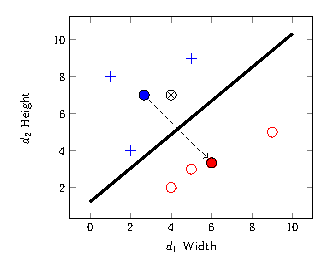
\includegraphics[width=0.7\linewidth,height=\textheight,keepaspectratio,alt={Linear classification with centroids, + denotes standing (positive) and denotes lying (negative). represents a centroid of the respective class. is a test instance.}]{chapters/../assets/figures/chapter07/fig-bin-lin-cent.pdf}

}

\caption{\label{fig-bin-lin_cent}Linear classification with centroids,
\(+\) denotes \emph{standing} (positive) and \(\circ\) denotes
\emph{lying} (negative). \(\bullet\) represents a centroid of the
respective class. \(\otimes\) is a test instance.}

\end{figure}%

With the identified linear function
\(f(v) = 1 + \frac{20}{27} v_1 - \frac{22}{27} v_2\), one can plug in
values of a test instance and make a prediction. If the result is
positive, it will predict positive (standing); otherwise, it will
predict negative (lying). For example, given a test instance at
\((4,7)\) (\(\otimes\) on Figure~\ref{fig-bin-lin_cent}), we can put the
values in the linear function and get:

\[\begin{aligned}
f(4,7)
& = & -1 - \frac{20}{27} \times 4 + \frac{22}{27} \times 7 \\
& = & \frac{47}{27} \\
& > & 0
\end{aligned}\]

The final result is positive -- the same positivity with the positive
class centroid -- and hence the test instance \(\otimes\) will be
classified into the \emph{standing} class.

Theoretically, we understand that the concept of \emph{standing} is on
the relation of \(height - width >0\) or, in terms of the linear
function, \(0 - v_1 + v_2 > 0\). The identified equation is a rough
approximation of this theoretical function. The model assumption about a
linear separation holds true in this example. But how precise we can
establish the exact linear function depends largely on the training
data. The data distribution influences the identification of related
parameters.

In particular, the centroid approach is greatly impacted by the density
of the training set and where most data instances are. For example,
having more data instances with smaller width and height in the negative
class change its centroid, which will, in turn, lead to a very different
linear function, illustrated in Figure~\ref{fig-bin-lin_cent2} (compare
to Figure~\ref{fig-bin-lin_cent}).

\begin{figure}

\centering{

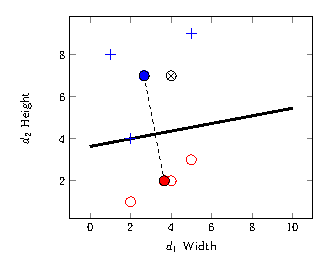
\includegraphics[width=0.7\linewidth,height=\textheight,keepaspectratio,alt={Linear classification with centroids, with smaller values in the negative class}]{chapters/../assets/figures/chapter07/fig-bin-lin-cent2.pdf}

}

\caption{\label{fig-bin-lin_cent2}Linear classification with centroids,
with smaller values in the negative class}

\end{figure}%

The centroid-based approach to linear classification is greatly
influenced by all data points in the training set and how they are
distributed. The basic assumption underlying the above modeling is that
the two classes are of the same size roughly and the "border" lies
halfway between their centers. This is often untrue and its performance
suffers.

\subsection{Support Vector Machines}\label{support-vector-machines}

Imagine settling the border between two countries, for example, the
United States and Canada. It does not matter where the centers of the
two countries are. Even if the two countries are of the same size, the
border is rarely halfway between the centers.

Rather, it is much more relevant to find out where cities, landmarks,
and populations are \emph{on the border}. For U.S. and Canada, cities
such as Seattle vs.~Detroit vs.~Vancouver, Detroit vs.~Toronto help
define their border.

For classification, it matters not where the centroids are but where the
\emph{borderline} data are. The Support Vector Machines, or SVM, is a
method focused on the border populations and draws the "border" based on
the so-called \emph{support vectors}, data points that are located on
the boundary and together form the border.

We start by connecting a number of data points within the same class to
construct a linear function, i.e.~a line on a 2-dimensional space, a
plane for 3 dimensions, and a hyperplane for higher dimensions. On the
2-dimensional shapes data, this means using any two points in each class
to form a straight line that, when used as the linear classification
function, satisfies two conditions: 1) all data points in the same class
fall on \emph{one size} of the linear function, and 2) most if not all
data points of the other class reside on the other side of the line. In
other words, if a line is drawn in the positive (standing class), then
1) data in it will test all positive (or all negative), and 2) data in
the other class will test the opposite, negative (or conversely
positive).

\begin{figure}

\centering{

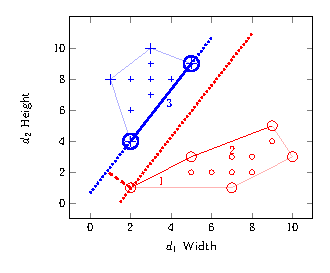
\includegraphics[width=0.7\linewidth,height=\textheight,keepaspectratio,alt={Linear classification with SVM, one candidate margin}]{chapters/../assets/figures/chapter07/fig-bin-svm.pdf}

}

\caption{\label{fig-bin-svm}Linear classification with SVM, one
candidate margin}

\end{figure}%

Figure~\ref{fig-bin-svm} illustrates the idea with the shapes data.
\footnote{Please note additional data points than previously discussed
  in the illustration.} Pairwise lines drawn in the figure all satisfy
the \(1^{st}\) condition and collectively form a \emph{convex hull} for
each class. However, not all lines meet the \(2^{nd}\) condition. In
fact, only the lines marked \(1\), \(2\), and \(3\) meet both
conditions. They are candidate \emph{support vectors}.

For each of the three candidate lines, we can draw a line perpendicular
to it from any point in the other class. From this process, we can find
out the margin between that candidate support vector line and the other
class (convex hull), which is where the boundary can be defined. For
example, in Figure~\ref{fig-bin-svm}, the two dotted lines show the
margin between line \(\#3\) and the negative class.

\begin{figure}

\centering{

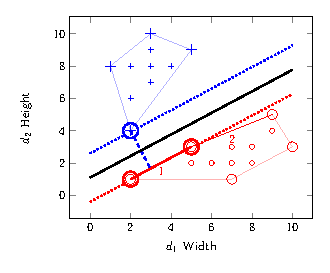
\includegraphics[width=0.7\linewidth,height=\textheight,keepaspectratio,alt={Linear classification with SVM, support vectors and maximum margin}]{chapters/../assets/figures/chapter07/fig-bin-svm2.pdf}

}

\caption{\label{fig-bin-svm2}Linear classification with SVM, support
vectors and maximum margin}

\end{figure}%

Yet a greater margin -- in fact the greatest margin of all -- can be
found between line \(\#1\) and point \((2,4)\) in the positive class, as
the two dotted lines in Figure~\ref{fig-bin-svm2} show. The greatest
margin will be chosen as the decision boundary, which is defined by a
few data points known as the \emph{support vectors}. As shown as circled
data points in Figure~\ref{fig-bin-svm2}, support vectors are those that
determine the maximum margin between the two \emph{convex hulls} of the
two classes.

With this, it is now easy to identify the linear equation in the margin
to separate the two classes. In Figure~\ref{fig-bin-svm2}, for example,
the solid line at \(v_2 = 1.1 + 0.667 v_1\) can be used as the linear
classifier. One can certainly use the linear functions on the support
vectors for classification as well, e.g.~to predict one class
vs.~another if a test instance is within the support vector boundary or
to estimate a probability if it is on the margin.

Note that with the shapes data example, we only have to deal with two
dimensions and any linear equation is a straight line. With a higher
dimensionality, the process remains the same mathematically but a linear
function becomes a plane or hyperplane. On three dimensions, for
example, three data points should be connected to construct a linear
equation (plane) to identify the convex hulls and support vectors.
Chapter~ has details on the mathematics for SVM.

\subsection{Perceptron: Toward a Neural
Network}\label{perceptron-toward-a-neural-network}

The linear function \(f(v)=w_0 + w_1 v_1 + w_2 v_2\) can be visualized
as a \emph{perceptron} in Figure~\ref{fig-bin-perceptron}, where the
node at \(\sum\) computes the weighted sum of input variables.
Obviously, this can be extended to include any number of variables \(m\)
for which \(f(v)=\sum_{i=1}^{m} w_i v_i\).

\begin{figure}

\centering{

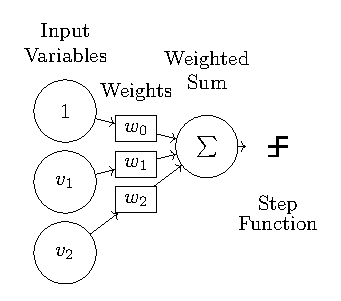
\includegraphics[width=0.7\linewidth,height=\textheight,keepaspectratio,alt={Linear classification with a Perceptron, where the output is a step function based on the weighted sum of input variables}]{chapters/../assets/figures/chapter07/fig-bin-perceptron.pdf}

}

\caption{\label{fig-bin-perceptron}Linear classification with a
Perceptron, where the output is a step function based on the weighted
sum of input variables}

\end{figure}%

A perceptron is a simple, one-layer neural network -- besides the input
variables, there is only one layer of nodes (only one \(\sum\) node) in
the model, as shown in Figure~\ref{fig-bin-perceptron}. The final output
of the perceptron is binary \(0\) or \(1\) by using a step function,
which simply converts values higher than a threshold to \(1\) and those
lower to \(0\). For example, one can use \(0\) as the threshold for a
step function \(f(s)\):

\[\begin{aligned}
  f(s) & = &
  \begin{cases}
  1 & \text{if } s>0\\
  0 & \text{otherwise}
  \end{cases}
\end{aligned}\]

which is visualized in Figure~\ref{fig-bin-step}.

\begin{figure}

\centering{

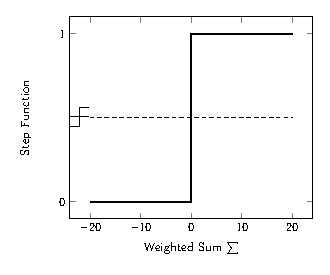
\includegraphics[width=0.7\linewidth,height=\textheight,keepaspectratio,alt={Example of a step function. Output is 0 for any value below zero, and is 1 if above zero.}]{chapters/../assets/figures/chapter07/fig-bin-step.pdf}

}

\caption{\label{fig-bin-step}Example of a step function. Output is \(0\)
for any value below zero, and is \(1\) if above zero.}

\end{figure}%

Before training, the weights are unknown and should be initialized with
certain values, e.g.~all \(0\). For each training instance, its values
\(v_1\) and \(v_2\) will be fed into the input layer and multiplied with
their weights \(w_1\) and \(w_2\) respectively.

Note that in Figure~\ref{fig-bin-perceptron}, the input with weight
\(w_0\) is always \(1\) for every training instance. This is referred to
as the \emph{bias}, which adds the constant \(w_0\) to the linear
function. Once every input is multiplied by its weight, the output
computes the sum of the weighted values.

For the shapes data, we can decide that the model will predict positive
(standing) if the output is greater than \(0\); negative (lying) if
otherwise. During training, if a correct prediction is made, the model
will have no need to adjust its weights (for now) and will simply move
to the next training instance.

If a misclassification occurs, however, the model will have to adjust
its weights so it can potentially make more correct predictions in the
future. When the model predicts negative on an actual positive instance,
the weights should be adjusted so the overall output (sum) will move
toward the positive side; and vice versa.

For example, for a specific shape instance with \(v_1\) (width) and
\(v_2\) (height) values, which is \((1, v_1, v_2)\) with the bias input
included. Suppose \(v_2>v_1\) and this instance actually belongs to the
positive (standing) class. Now if the model finds out
\(w_0 + w_1 v_1 + w_2 v_2 < 0\) and predicts negative (lying). We will
add the input values to their current weights:

\[\begin{aligned}
w'_0 & \gets & w_0 + 1 \\
w'_1 & \gets & w_1 + v_1 \\
w'_2 & \gets & w_2 + v_2
\end{aligned}\]

where \(w'\) is the updated weight. Because \(v_2>v_1\), the weight for
height \(w_2\) will increase more than the weight for width \(w_1\).

Conversely, for a training instance with \(v_1>v_2\) that actually
belongs to the negative (lying) class, if it is misclassified as
positive, then the current weights will be reduced by the input values:

\[\begin{aligned}
w'_0 & \gets & w_0 - 1 \\
w'_1 & \gets & w_1 - v_1 \\
w'_2 & \gets & w_2 - v_2
\end{aligned}\]

Now that \(v_1>v_2\), the weight for width \(w_1\) will be reduced more
than \(w_2\). The training continues for a number of iterations or until
the weights stabilize. With more training instances and
misclassifications, the weights will be adjusted further, leading to
relatively a greater (positive) value of \(w_2\) and a smaller
(negative) value of \(w_1\).

Theoretically, we know that the classification function for
\emph{standing} vs.~\emph{lying} should be in the form of
\(f(v) = 0 - v_1 + v_2\), with \(w_1\) and \(w_2\) having opposite
signs. Overall, the adjustment of weights discussed above is moving in
the correct direction. As for the \emph{bias}, it will simply be
adjusted back and forth with positive and negative misclassifications.
For the shapes data, \(w_0\) will be more or less canceled out and its
absolute value will become much smaller than those of \(w_1\) and
\(w_2\).

The \emph{perception} model is learning by \emph{mistakes}, as it
updates the weights only when there is misclassification. For classes
that are linearly separable, the updating strategy is guaranteed to
converge on a set of weights.

\section{Non-Linear Models}\label{non-linear-models}

Many machine learning problems in the real world cannot be solved by a
linear equation. Consider the car evaluation data in
Table~\hyperref[tab-bin-car]{1.2}.

\protect\phantomsection\label{tab-bin-car}
\begin{longtable}[]{@{}ccl@{}}
\caption{Car evaluation data. Buying price and maintenance cost are on a
scale of \(1\) to \(4\), with \(1\) meaning the lowest price (cost) and
\(4\) the highest.}\tabularnewline
\toprule\noalign{}
Buying Price & Maintenance Cost & Evaluation \\
\midrule\noalign{}
\endfirsthead
\toprule\noalign{}
Buying Price & Maintenance Cost & Evaluation \\
\midrule\noalign{}
\endhead
\bottomrule\noalign{}
\endlastfoot
2 & 2 & Acceptable \\
2 & 1 & Acceptable \\
1 & 2 & Acceptable \\
1 & 1 & Acceptable \\
4 & 4 & Unacceptable \\
4 & 3 & Unacceptable \\
4 & 2 & Unacceptable \\
4 & 1 & Unacceptable \\
3 & 4 & Unacceptable \\
3 & 3 & Unacceptable \\
3 & 2 & Unacceptable \\
3 & 1 & Unacceptable \\
2 & 4 & Unacceptable \\
2 & 3 & Unacceptable \\
1 & 4 & Unacceptable \\
1 & 3 & Unacceptable \\
\end{longtable}

In the data, the concept is about whether a car is \emph{acceptable} or
\emph{unacceptable} given its \emph{buying price} and \emph{maintenance
cost}.\footnote{The tiny data set was inspired by the UCI's Car
  Evaluation collection. However, this simplified version is intended
  for demonstration only and does not represent the actual data in the
  UCI repository.} The price (cost) variables are on an ordinal scale:
low, medium, high, and very high, which we convert into an
equal-interval numeric scale from \(1\) (low) to \(4\) (very high).

While it is possible to include other variables such as the number of
doors and safety features, we will focus on the cost factors in the
discussion here. Figure~\ref{fig-bin-car} plots \emph{maintenance cost}
vs.~\emph{buying price}, with the \(+\) indicating an \emph{acceptable}
car and \(\circ\) unacceptable. The two classes appear not separable
linearly on the two-dimensional space -- that is, there is no straight
line that can be drawn to separate the two.

Again, if one can introduce other predictor variables and the classes
might be separable linearly on a higher-dimensional space. But even with
the only two variables, namely \emph{maintenance cost} and \emph{buying
price}, the plot seems to suggest that a car will be evaluated
\emph{unacceptable} with either a high buying price or a high
maintenance cost.

Perhaps one can draw two straight lines, one to separate the classes on
the price dimension and the other on the maintenance cost. However, this
is no longer one linear equation of the two variables that can fit in
with a linear model. Alternatively, we can still draw a curve (a
non-linear function) to separate them. For example, as shown as the
dashed line in Figure~\ref{fig-bin-car}, a circular function such as
\((v_1-1)^2 + (v_2 -1)^2 = 3\) can set the boundary between the two
classes. The question is: how can we identify such as a non-linear
function from the training data?

\begin{figure}

\centering{

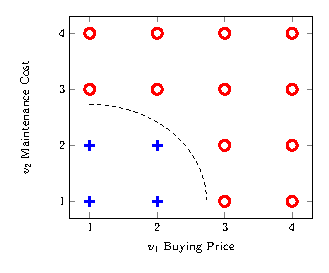
\includegraphics[width=0.7\linewidth,height=\textheight,keepaspectratio,alt={Car evaluation data. + is the positive (acceptable) class and is the negative (unacceptable).}]{chapters/../assets/figures/chapter07/fig-bin-car.pdf}

}

\caption{\label{fig-bin-car}Car evaluation data. \(+\) is the positive
(acceptable) class and \(\circ\) is the negative (unacceptable).}

\end{figure}%

\subsection{Kernel SVM}\label{kernel-svm}

We have discussed the \emph{support vector machines}, which, in its
original form, is a linear model. How can we apply SVM to non-linear
data? Now instead of finding out a non-linear function, we can think
about how the data can be transformed in such a way that they are
linearly separable.

In particular, we can map the data onto a higher dimensional space with
richer features, where a linear classifier is applicable. Now that we do
not have additional variables, how can we create a higher-dimensional
space? The basic idea is to find non-linear combinations of existing
variables, via a so-called \emph{kernel} function. We will have an
in-depth discussion of \emph{kernel} functions in Chapter~. But in the
nutshell, a \emph{kernel} function can be computed by a dot product with
expanded features and makes it extremely efficient to identify the
decision hyperplane in the higher dimensional space.

Among families of kernel functions, a polynomial function is often used.
For example, we may consider a quadratic transformation with the car
evaluation data. Given the two existing variables, any data instance
with \(v = (v_1, v_2)\) (a two-dimensional vector) can be expanded onto
a vector with more dimensions:

\[\begin{aligned}
  \phi(v) & = & (v_1^2, v_2^2, \sqrt{2} v_1 v_2)
\end{aligned}\]

Note that the quadratic expansion should result in \(5\) dimensions
including the original dimensions of \(v_1\) and \(v_2\). We focus on
the \(3\) additional features and thus limit the number of dimensions to
three, which can be visualized.

With the \(v_1^2\) and \(v_2^2\) transformation, data in the two classes
already appear to be linearly separable. As shown in
Figure~\ref{fig-bin-car_q2}, the solid line at \(v_1+v_2-9=0\) can
separate the data we have so far. However, this does not necessarily
represent the general idea of car evaluation and new data may violate
the rule (cross the decision boundary).

\begin{figure}

\centering{

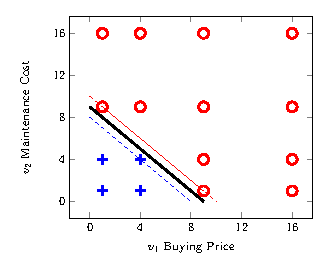
\includegraphics[width=0.7\linewidth,height=\textheight,keepaspectratio,alt={Car evaluation data, with transformed v\_1\^{}2 and v\_2\^{}2.}]{chapters/../assets/figures/chapter07/fig-bin-car-q2.pdf}

}

\caption{\label{fig-bin-car_q2}Car evaluation data, with transformed
\(v_1^2\) and \(v_2^2\).}

\end{figure}%

Whether a car is acceptable or not may depend on some form of
interaction between the buying price and maintenance cost. With the
quadratic expansion, the additional dimension of \(\sqrt{2} v_1 v_2\)
can be seen as an interaction variable in the form of multiplication.

When all three expanded features are considered, the data are mapped to
a three-dimensional space shown in Figure~\ref{fig-bin-car_q3}, where
they may be separated linearly. Of all linear equations (planes) formed
by any three points in each class, we have identified two planes closest
to their opposite classes.

\begin{figure}

\centering{

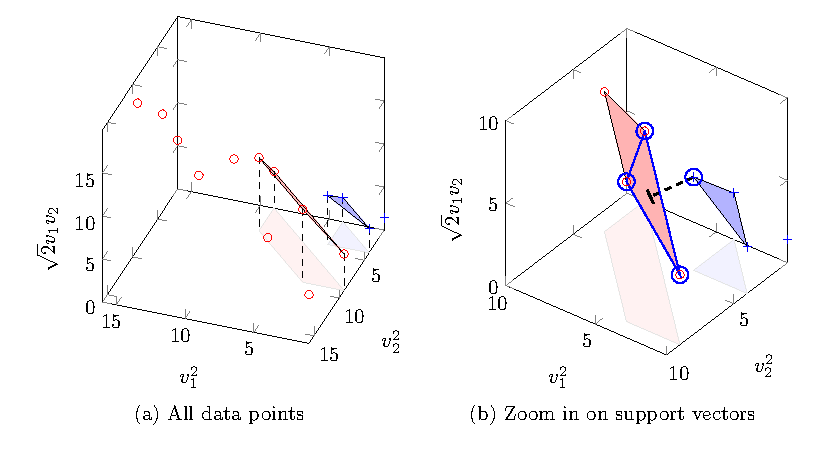
\includegraphics[width=0.7\linewidth,height=\textheight,keepaspectratio,alt={Car evaluation data, mapped to higher dimensions with v\_1\^{}2, v\_2\^{}2, and 2 v\_1 v\_2. The two planes are closest to the opposite class. The projected shadows are for reference only. (a) shows all data points in the three dimensional space, and (b) is a closer view of the two planes with support vectors. Dashed line is the gap (margin) between the two classes. Circled data points are support vectors.}]{chapters/../assets/figures/chapter07/fig-bin-car-q3.pdf}

}

\caption{\label{fig-bin-car_q3}Car evaluation data, mapped to higher
dimensions with \(v_1^2\), \(v_2^2\), and \(\sqrt{2} v_1 v_2\). The two
planes are closest to the opposite class. The projected shadows are for
reference only. (a) shows all data points in the three dimensional
space, and (b) is a closer view of the two planes with support vectors.
Dashed line is the gap (margin) between the two classes. Circled data
points are support vectors.}

\end{figure}%

Figure~\ref{fig-bin-car_q3} (a) shows all data points in the expanded
dimensional space with quadratic mapping. The two planes formed by data
points are the closest to the opposite class, which are candidate
support vectors. Shadows of the planes are projected to the "ground"
(i.e.~\(v_2^2\) vs.~\(v_1^2\) dimensions) for easier reading of related
data points.

Figure~\ref{fig-bin-car_q3} (b) zooms in on the planes formed by
candidate support vectors in the three-dimensional space, where a
decision boundary can be identified to maximize the margin between the
two classes (convex hulls). The dashed line connects the closest points
of data in the two classes (convex hulls), by drawing a line from the
circled positive point perpendicular to the plane formed by three
circled negative points. The four circled points (one positive and three
negative) are the identified support vectors, based on which the margin
is established and classification can be performed.

Besides polynomial kernels, other popular kernel functions for SVM
include radial basis and string kernels. A string kernel, for example,
operates directly on symbol sequences without vectorized features and is
useful in applications such as text classification and gene sequence
analysis.

\subsection{Multi-Layer Neural
Networks}\label{multi-layer-neural-networks}

We know the single perceptron can only be applied to linearly separable
data. The car evaluation data, as shown in Figure~\ref{fig-bin-car},
cannot be separated by one linear function. However, with a step
function, one can transform the data into something linearly separable.
Specifically, for a value \(s\) on the \(v_1\) or \(v_2\) dimension, we
use the following step function:

\[\begin{aligned}
  f(s) & = &
  \begin{cases}
  1 & \text{if } s>2.5\\
  0 & \text{otherwise}
  \end{cases}
\end{aligned}\]

So it returns \(1\) for a value above \(2.5\), and \(0\) for a value
below. Applying the step function to both \(v_1\) (buying price) and
\(v_2\) (maintenance cost), we have transformed data in
Figure~\ref{fig-bin-car_step}. All positive (acceptable) data have been
mapped to the \((0,0)\) point whereas the negative (unacceptable) ones
are at \((0,1)\), \((1,1)\), and \((1,0)\). As the solid line in
Figure~\ref{fig-bin-car_step} shows, the transformed data are now
linearly separable.

\begin{figure}

\centering{

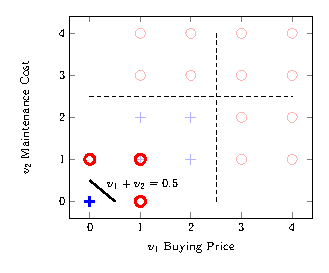
\includegraphics[width=0.7\linewidth,height=\textheight,keepaspectratio,alt={Car evaluation data, transformed by a step function. A step function with a threshold 2.5 converts the original data (+ and in faded colors) to those with 0 and 1 values (+ and in bright colors). The solid line at v\_1+v\_2=0.5 separate the two classes.}]{chapters/../assets/figures/chapter07/fig-bin-car-step.pdf}

}

\caption{\label{fig-bin-car_step}Car evaluation data, transformed by a
step function. A step function with a threshold \(2.5\) converts the
original data (\(+\) and \(\circ\) in faded colors) to those with \(0\)
and \(1\) values (\(+\) and \(\circ\) in bright colors). The solid line
at \(v_1+v_2=0.5\) separate the two classes.}

\end{figure}%

This non-linear classification with step function transformation can be
represented with a multi-layer neural network. As shown in
Figure~\ref{fig-bin-nn}, each of the input variables \(v_1\) and \(v_2\)
is normalized by a step function and then multiplied by \(-1\) before
feeding into the final output, which is combined with the bias weighted
\(0.5\). This is equivalent to
\(0.5 \times 1 -1\times f(v_1) - 1\times f(v_2)\), where \(f\) is the
step function for \(v_1\) and \(v_2\) values.

\begin{figure}

\centering{

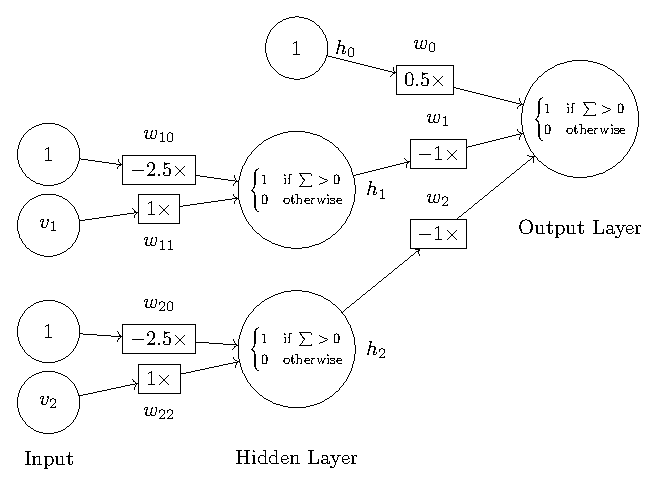
\includegraphics[width=0.7\linewidth,height=\textheight,keepaspectratio,alt={Multi-layer neural network with step functions. represents the weighted sum of input values leading to the present node.}]{chapters/../assets/figures/chapter07/fig-bin-nn.pdf}

}

\caption{\label{fig-bin-nn}Multi-layer neural network with step
functions. \(\sum\) represents the weighted sum of input values leading
to the present node.}

\end{figure}%

For example, with data point \((2,2)\), the step function will convert
them into \((0,0)\). With the bias \(0.5\times1\), the weighted sum is
\(0.5\times1 - 1\times 0 - 1\times 0 = 0.5\) and it will be classified
positive (acceptable). With data point \((3,1)\), it is transformed into
\((1,0)\) by the step function and the final weighted sum is
\(0.5\times1 - 1\times 1 - 1\times 0 = -0.5\), which will be classified
negative (unacceptable).

Using the multi-layer neural network, based on the additional hidden
layer with step functions between the input and final output, it is now
possible to establish a non-linear model such as the one in
Figure~\ref{fig-bin-nn}.

But the question remains -- how can the weights of the model, together
with the step function, be identified properly? While it is tempting to
use a similar strategy as with the single perceptron, the non-linearity
of the model rules out such a linear strategy for weight adjustment.
That is, simply adding or subtracting weights (linear combinations) does
not help when the model is non-linear.

Can we adjust the weights in a non-linear manner during training? In
other words, can we adjust the weights based on how much each variable
contributes to the final output via the hidden layer? The general
optimization technique called \emph{gradient descent} makes it possible
to find optimal values (weights) by searching in the derivatives of
related functions. However, a step function, as illustrated in
Figure~\ref{fig-bin-step}, has a sudden jump (not smooth transition)
between \(0\) and \(1\) and is not differentiable.

If we are to retain the idea of a step function, can we develop one that
functions in the like manner and yet smooth and differentiable? A
candidate is the \emph{sigmoid} function, which is defined by:

\[\begin{aligned}
  f(v) & = & \frac{1}{1+e^{-v}}
\end{aligned}\]

for a value \(v\). Figure~\ref{fig-bin-sigmoid} shows the functional
curve of sigmoid, which transforms the weighted sum of a node to a value
approaching \(0\) or \(1\). The threshold is \(0\) by default but we can
use any threshold for the transformation. For example, with a threshold
of \(5\), the sigmoid function becomes:

\[\begin{aligned}
  f(v) & = & \frac{1}{1+e^{-(v-5)}}
\end{aligned}\]

which shifts the functional curve on the \(x\) coordinates by \(+5\)
(dashed line in Figure~\ref{fig-bin-sigmoid}).
\(v-5 = 1\times v + (-5)\times 1\) is equivalent to the weighted sum of
variable \(v\) (with weight \(w=1\)) and bias \(1\) (with weight
\(w_0=-5\)). It can be generalized as a linear function of any number of
input variables with bias in the form of
\(\sum = w_0 + \sum_i w_i v_i\).

\begin{figure}

\centering{

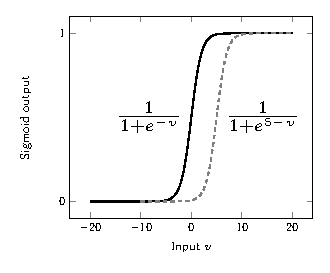
\includegraphics[width=0.7\linewidth,height=\textheight,keepaspectratio,alt={Sigmoid function}]{chapters/../assets/figures/chapter07/fig-bin-sigmoid.pdf}

}

\caption{\label{fig-bin-sigmoid}Sigmoid function}

\end{figure}%

Now if we replace the step function with the sigmoid function in
Figure~\ref{fig-bin-nn}, we have the multi-layer neural network in
Figure~\ref{fig-bin-nn_sigmoid}, in which each layer (node) is
differentiable and the weight can be learned by gradient descent.

\begin{figure}

\centering{

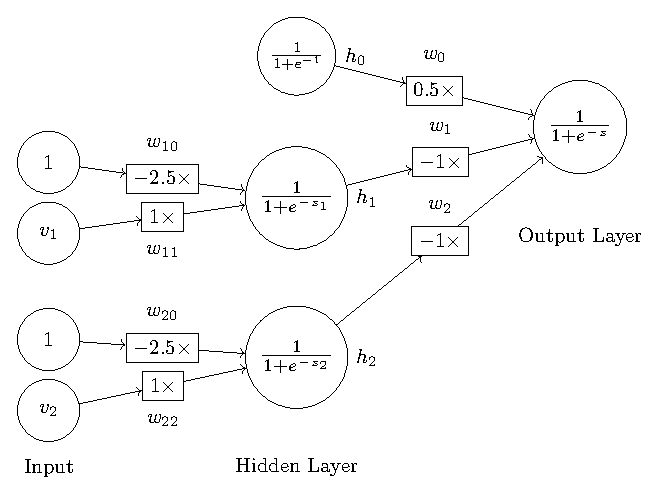
\includegraphics[width=0.7\linewidth,height=\textheight,keepaspectratio,alt={Multi-layer neural network with the sigmoid function. s\_1 and s\_2 are the weighted sum of input values leading to the respective hidden nodes whereas s is the weighted sum of input values leading to the output layer.}]{chapters/../assets/figures/chapter07/fig-bin-nn-sigmoid.pdf}

}

\caption{\label{fig-bin-nn_sigmoid}Multi-layer neural network with the
sigmoid function. \(s_1\) and \(s_2\) are the weighted sum of input
values leading to the respective hidden nodes whereas \(s\) is the
weighted sum of input values leading to the output layer.}

\end{figure}%

The weighted sum for each hidden node \(i\) can be computed by:

\[\begin{aligned}
  s_i & = & \sum_{j=0}^{m} w_{ij} v_j
\end{aligned}\]

where \(m\) is the number of variables and \(v_0\) is the bias, which is
always \(1\). Given the sigmoid function \(f\), the output of each node
in the hidden layer is:

\[\begin{aligned}
  h_i
  & = & f(s_i) \\
  & = & f(\sum_{j=0}^{m} w_{ij} v_j)
\end{aligned}\]

In Figure~\ref{fig-bin-nn_sigmoid}, this can be written as:

\[\begin{aligned}
  h_1
  & = & f(\sum_{j=0}^{m} w_{1j} v_j) \\
  & = & f(w_{10} v_0 + w_{11} v_1 + w_{12} v_2) \\
  & = & f(-2.5\times1 + 1\times v_2 + 0\times v_2) \\
  h_2
  & = & f(\sum_{j=0}^{m} w_{2j} v_j) \\
  & = & f(w_{20} v_0 + w_{21} v_1 + w_{22} v_1) \\
  & = & f(-2.5\times1 + 0\times v_2 + 1\times v_2)
\end{aligned}\]

The final output, predicted value \(\hat{y}\), is the sigmoid of the
weighted sum of values from the hidden layer:

\[\begin{aligned}
  \hat{y}
  & = & f(s) \\
  & = & f(\sum_{i=0}^{m} w_i h_i) \\
  & = & f\Big(\sum_{i=0}^{m} w_i f\big(\sum_{j=0}^{m} w_{ij} v_j\big)\Big)
\end{aligned}\]

which, for the model in Figure~\ref{fig-bin-nn_sigmoid}, can be computed
by:

\[\begin{aligned}
  \hat{y}
  & = & f(w_0 h_0 + w_1 h_1 + w_2 h_2) \\
  & = & f\Big(w_0 f(1) \\
  &   & + w_1 f\big(w_{10} + w_{11} v_1 + w_{12} v_2\big) \\
  &   & + w_2 f\big(w_{20} + w_{21} v_1 + w_{22} v_2\big)\Big)
\end{aligned}\]

Let \(y\) be the actual outcome (class \(0\) or \(1\)) for input from
the hidden layer \(h\). If we define the error \(E\) as a squared
function:

\[\begin{aligned}
  E(h) & = & \frac{1}{2} (y - \hat{y})^2
\end{aligned}\]

For a prediction based on the sigmoid function \(f\), it can be shown
that the differential with respect to a weight \(w_i\) to the output
layer is:

\[\begin{aligned}
  \frac{dE(h)}{dw_i}
  & = & \big( f(s) - y \big) f'(s) f(s_i) \\
  & = & \big( f(s) - y \big) f'(s) h_i
\end{aligned}\]

where \(s\) is the weighted sum at the output layer and \(f'(s)\) is the
derivative of the sigmoid function \(f(s)\), which is as simple as
\(f(s)(1-f(s))\). This gives the differentials needed to optimize
\(w_i\) weights from the hidden layer to the output, i.e.~\(w_0\),
\(w_1\), and \(w_2\) weights in Figure~\ref{fig-bin-nn_sigmoid}.

Now that values in the hidden layer \(h\) are based on weighted sums of
the input layer, we also need to optimize \(w_{ij}\) weights connecting
the input to the hidden layer. Given input values \(v\), the
differential with respect to a weight \(w_{ij}\) to hidden node \(h_i\)
can be computed by:

\[\begin{aligned}
  \frac{dE(v)}{dw_{ij}}
  & = & \big( f(s) - y \big) f'(s) f'(s_i) v_j
\end{aligned}\]

The differentials will be used to update weights to both layers during
the training process. In particular, the differential
\(\frac{dE(h)}{dw_i}\) in
Equation~\hyperref[eq-bin-dwi]{{[}eq-bin-dwi{]}} will be used to
subtract from existing weights of \(w_0\), \(w_1\), and \(w_2\). The
differential \(\frac{dE(v)}{dw_{ij}}\) in
Equation~\hyperref[eq-bin-dwij]{{[}eq-bin-dwij{]}} will be used to
subtract from existing weights of \(w_{10}\) and \(w_{11}\) for \(h_1\);
\(w_{20}\) and \(w_{22}\) for \(h_2\) in
Figure~\ref{fig-bin-nn_sigmoid}. This approach of revising weights to
the two layers can thought of as propagating differentials of squared
errors \emph{backward} in the feed-forward neural network, and is
referred to as \emph{backpropagation}.

To understand how backpropagation actually operates, let's walk through
the training process with the first data instance in
Table~\hyperref[tab-bin-car_nn]{1.3}.

\protect\phantomsection\label{tab-bin-car_nn}
\begin{longtable}[]{@{}ccl@{}}
\caption{Car evaluation, training data for multi-layer neural network.
Evaluation value \(1\) for \emph{acceptable} and \(0\) for
unacceptable.}\tabularnewline
\toprule\noalign{}
Buying Price & Maintenance Cost & Evaluation \\
\midrule\noalign{}
\endfirsthead
\toprule\noalign{}
Buying Price & Maintenance Cost & Evaluation \\
\midrule\noalign{}
\endhead
\bottomrule\noalign{}
\endlastfoot
\textbf{2} & \textbf{2} & \textbf{1} \\
.. & .. & .. \\
\end{longtable}

Before training, we don't know the weights and may initialize them with
all \(0\) values. Note that we use \(0\) initial weights for easy
demonstration. This is not necessarily the best strategy for
initialization.

\begin{figure}

\centering{

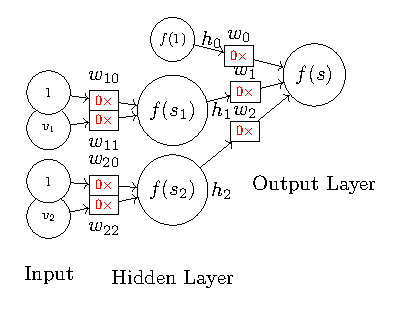
\includegraphics[width=0.7\linewidth,height=\textheight,keepaspectratio,alt={Backpropagation step 1 with 0 initial weights.}]{chapters/../assets/figures/chapter07/fig-bin-nn-sigmoid-0.pdf}

}

\caption{\label{fig-bin-nn_sigmoid_0}Backpropagation step 1 with \(0\)
initial weights.}

\end{figure}%

Now with the model and initial weights in
Figure~\ref{fig-bin-nn_sigmoid_0}, given the first training instance of
\((2,2)\), we can compute:

\[\begin{aligned}
  h_0
  & = & f(1) \\
  & = & \frac{1}{1+e^{-1}} \\
  & = & 0.731 \\
  h_1
  & = & f(s_1) \\
  & = & f(0\times1 + 0\times2) \\
  & = & 0.5 \\
  h_2
  & = & f(s_2) \\
  & = & f(0\times1 + 0\times2) \\
  & = & 0.5
\end{aligned}\]

The final prediction \(\hat{y}\) is computed by:

\[\begin{aligned}
  f(s)
  & = & f(0\times0.731 + 0\times0.5 + 0\times0.5) \\
  & = & f(0) \\
  & = & 0.5
\end{aligned}\]

We get:

\[\begin{aligned}
  \big( f(s) - y \big) f'(s)
  & = & \big( f(s) - y \big) f(s) \big( 1 - f(s)\big) \\
  & = & (0.5 - 1) \times 0.5 \times (1 - 0.5) \\
  & = & - 0.125
\end{aligned}\]

With the actual class being \(1\), we can compute the differentials. For
each \(w_i\) weight leading to the output layer:

\[\begin{aligned}
  \frac{dE(h)}{dw_0}
  & = & \big( f(s) - y \big) f'(s) h_0 \\
  & = & -0.125 \times h_0 \\
  & = & -0.125 \times 0.73 \\
  & = & -0.0914 \\
  \frac{dE(h)}{dw_1}
  & = & -0.125 \times 0.5 \\
  & = & -0.0625 \\
  \frac{dE(h)}{dw_2} & = & -0.0625 \\
\end{aligned}\]

Subtracting these (negative) values from their current weights
respectively, we obtain the new weights \(w_0=0.0914\), \(w_1=0.0625\),
and \(w_2 = 0.625\).

Now we can further back-propagate the error to the \(w_{ij}\) weights
from the input layer:

\[\begin{aligned}
  \frac{dE(v)}{dw_{10}}
  & = & \big( f(s) - y \big) f'(s) f'(s_1) v_0 \\
  & = &  -0.125 \times f(s_1) (1 - f(s_1)) v_0 \\
  & = &  -0.125 \times 0.5 \times (1-0.5) \times 1 \\
  & = & -0.0313 \\
  \frac{dE(v)}{dw_{11}}
  & = & \big( f(s) - y \big) f'(s) f'(s_1) v_1 \\
  & = & -0.125 \times 0.5 \times (1-0.5) \times 2 \\
  & = & -0.0625 \\
  \frac{dE(v)}{dw_{20}}
  & = & -0.0313 \\
  \frac{dE(v)}{dw_{22}}
  & = & -0.0625
\end{aligned}\]

Subtracting these from current \(0\) values, we obtain new weights for
of all \(w_{ij}\), namely \(w_{10}=0.0313\) and \(w_{11}=0.0625\) to
hidden node \(h_1\), and \(w_{20}=0.0313\) and \(w_{22}=0.0625\) for
hidden node \(h_2\).

\begin{figure}

\centering{

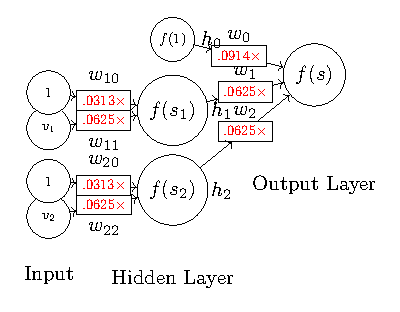
\includegraphics[width=0.7\linewidth,height=\textheight,keepaspectratio,alt={Backpropagation step 2 with updated weights}]{chapters/../assets/figures/chapter07/fig-bin-nn-sigmoid-1.pdf}

}

\caption{\label{fig-bin-nn_sigmoid_1}Backpropagation step 2 with updated
weights}

\end{figure}%

Figure~\ref{fig-bin-nn_sigmoid_1} shows the model with updated weights
after training by the first instance \((2,2)\) with a known class label
\(1\). We can continue to train the model with additional data instances
in Table~\hyperref[tab-bin-car_nn]{1.3}. This can be repeated with the
same data until weights are stabilized and the error is reduced to a
certain level.

\begin{figure}

\centering{

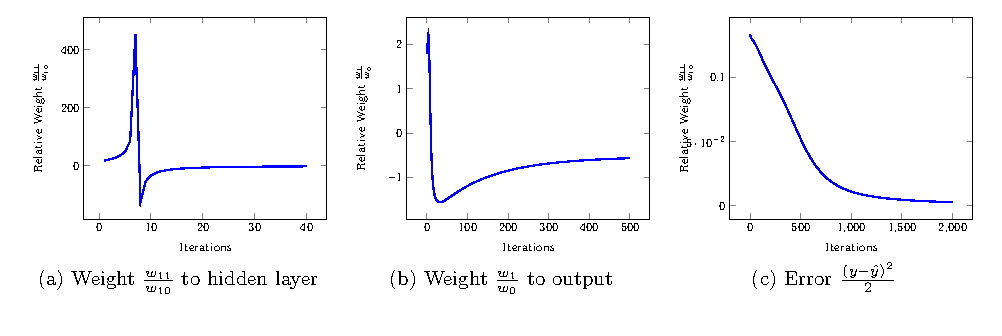
\includegraphics[width=0.7\linewidth,height=\textheight,keepaspectratio,alt={Neural network training iterations and convergence}]{chapters/../assets/figures/chapter07/fig-bin-car-nn-converge.pdf}

}

\caption{\label{fig-bin-car_nn_converge}Neural network training
iterations and convergence}

\end{figure}%

Figure~\ref{fig-bin-car_nn_converge} shows relative weights and error
over time, via iterations of repeated training with data in
Table~\hyperref[tab-bin-car_nn]{1.3}. Note that in linear equations,
absolute values of related weights (coefficients) are not important.
Rather, it is their relative weight to one another that matters. Hence,
we present weights relative to \(w_0\), i.e.~divided by the \emph{bias}
weight.

Overall, the figures show the weights and error all appear to converge.
However, they seem to differ in the number of iterations needed for
their convergence. In Figure~\ref{fig-bin-car_nn_converge} (a), the
relative weight of \(w_{11}\) (the weight of \(v_1\) to the hidden node
\(h_1\)) fluctuates a lot in the first \(10\) iterations but stabilizes
quickly after a few dozen iterations. In
Figure~\ref{fig-bin-car_nn_converge} (b), \(w_1\) -- the weight from the
hidden node \(h_1\) to the final output -- appears to take hundreds of
iterations to converge. The squared error, as shown in
Figure~\ref{fig-bin-car_nn_converge} (c), takes even even more
iterations to be minimized.

In the end, we obtain the weights in
Table~\hyperref[tab-bin-car_nn_result]{{[}tab-bin-car\_nn\_result{]}}
with minimized squared error.

{\def\LTcaptype{none} % do not increment counter
\begin{longtable}[]{@{}ccccccccc@{}}
\toprule\noalign{}
Weights & \(w_0\) & \(w_1\) & \(w_2\) & \(w_{10}\) & \(w_{11}\) &
\(w_{20}\) & \(w_{22}\) & Error \\
\midrule\noalign{}
\endhead
\bottomrule\noalign{}
\endlastfoot
Absolute & -18.4 & 9.47 & 9.44 & 7.35 & -2.93 & 7.43 & -2.96 & 0.0027 \\
Relative & -1 & 0.52 & 0.52 & 1 & -0.40 & 1 & -0.40 & 0.0027 \\
Relative & -1.92 & 1 & 1 & 2.5 & -1 & 2.5 & -1 & 0.0027 \\
\end{longtable}
}

The result of
Table~\hyperref[tab-bin-car_nn_result]{{[}tab-bin-car\_nn\_result{]}}
can be represented as the final (converged) model in
Figure~\ref{fig-bin-car_nn_result}, which is highly similar to the one
in Figure~\ref{fig-bin-nn_sigmoid}. For example, the weighted sum for
hidden node \(h_1\) is \(2.5 - v_1\) in the model here, which is simply
the negative of what is in Figure~\ref{fig-bin-nn_sigmoid}, where the
sum is \(v_1 - 2.5\). We observe the same with the hidden node \(h_2\).
This leads to the different signs of \(w_1, w_2\) vs.~\(w_0\) to the
output layer.

\begin{figure}

\centering{

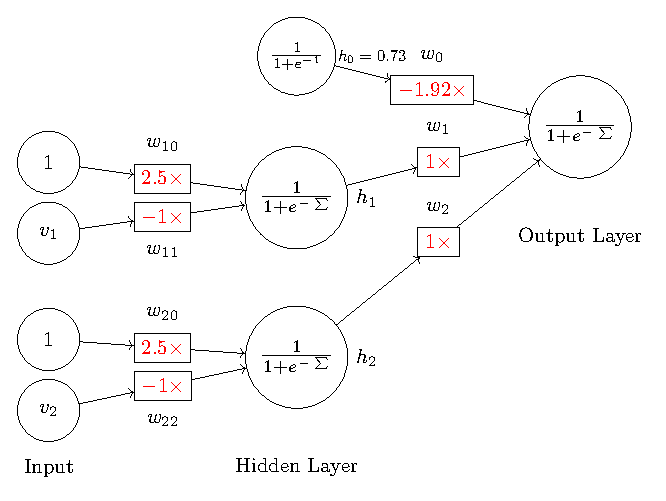
\includegraphics[width=0.7\linewidth,height=\textheight,keepaspectratio,alt={Neural network final model. Compare to the referenced figure. Note that we transform the bias node on the hidden layer with the sigmoid as well, i.e. h\_0 = f(1) = 11+e\^{}-1 = 0.73. In the final model, w\_0 h\_0 = -1.920.73=-1.4.}]{chapters/../assets/figures/chapter07/fig-bin-car-nn-result.pdf}

}

\caption{\label{fig-bin-car_nn_result}Neural network final model.
Compare to the referenced figure. Note that we transform the bias node
on the hidden layer with the sigmoid as well,
i.e.~\(h_0 = f(1) = \frac{1}{1+e^{-1}} = 0.73\). In the final model,
\(w_0 h_0 = -1.92\times0.73=-1.4\).}

\end{figure}%

Figure~\ref{fig-bin-car_nn_result_plot} visualizes how the model
transforms the original data into something separable. A sigmoid
function with a weighted sum of \(2.5 - v\) (for both \(v_1\) and
\(v_2\)) converts the original data (\(+\) and \(\circ\) in faded
colors) to values close to \(0\) (if \(v>2.5\)) and \(1\) values (if
\(v<2.5\)).

\begin{figure}

\centering{

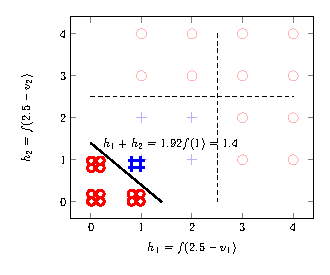
\includegraphics[width=0.7\linewidth,height=\textheight,keepaspectratio,alt={Visualization of the final model on car evaluation. Data transformed by the sigmoid function h\_i = f(s\_i) = 11+e\^{}-s\_i, where s\_i is the weighted sum of each hidden node: s\_1=2.5 - v\_1 and s\_2 = 2.5 - v\_2. The solid line at h\_1+h\_2 - 1.92 f(1)=0 is where the sigmoid of the output layer makes the cut.}]{chapters/../assets/figures/chapter07/fig-bin-car-nn-result-plot.pdf}

}

\caption{\label{fig-bin-car_nn_result_plot}Visualization of the final
model on car evaluation. Data transformed by the sigmoid function
\(h_i = f(s_i) = \frac{1}{1+e^{-s_i}}\), where \(s_i\) is the weighted
sum of each hidden node: \(s_1=2.5 - v_1\) and \(s_2 = 2.5 - v_2\). The
solid line at \(h_1+h_2 - 1.92 f(1)=0\) is where the sigmoid of the
output layer makes the cut.}

\end{figure}%

Given the limited training data we have, there are many non-linear
solutions to the classification problem. In the end, we obtain the model
in Figure~\ref{fig-bin-car_nn_result} which is different from what we
proposed in Figure~\ref{fig-bin-nn_sigmoid}. Both models will make
perfect classifications on the training data presented in
Table~\hyperref[tab-bin-car_nn]{1.3}. However, a model thus obtained has
not necessarily found the global optimal. In fact, the back-propagation
mechanism via gradient descent can converge to a local optimum, which
depends on many factors such as the starting point (initial values) and
the sequence of training data. The learning rate also impacts the
convergence of weights and, occasionally, may also influence where they
converge.

\chapter{Multiclass and Structured Decisions}\label{ch-multiclass}

\section{From Binary to Multiple
Classes}\label{from-binary-to-multiple-classes}

\section{One-vs-Rest and One-vs-One
Strategies}\label{one-vs-rest-and-one-vs-one-strategies}

\section{Scores, Probabilities, and
Softmax}\label{scores-probabilities-and-softmax}

\section{Decision Trees and Rule-Based
Decisions}\label{decision-trees-and-rule-based-decisions}

\section{Multilabel and Ordinal
Outcomes}\label{multilabel-and-ordinal-outcomes}

\section{Error Analysis and
Calibration}\label{error-analysis-and-calibration}

\section{Summary, Exercises, and Lab}\label{summary-exercises-and-lab}

\chapter{Numeric Prediction and Regression}\label{ch-regression}

\section{Prediction with Continuous
Outcomes}\label{prediction-with-continuous-outcomes}

\section{Linear Regression}\label{linear-regression}

\section{Loss Functions and Fitting}\label{loss-functions-and-fitting}

\section{Regularization}\label{regularization}

\section{Nonlinear Regression}\label{nonlinear-regression}

\section{Uncertainty and Diagnostics}\label{uncertainty-and-diagnostics}

\section{Summary, Exercises, and Lab}\label{summary-exercises-and-lab-1}

\chapter{Clustering and Organization}\label{ch-clustering}

We as human organize things. An important aspect of human development is
to recognize the commonality of objects and group them together, for
example, in terms of shapes and colors.

A related category of machine learning algorithms is called
\emph{clustering}, which aims to bring like entities together and, by
doing so, discovers major groups, patterns, and themes in the data.
Clustering is often referred to as unsupervised learning because its
outcome is not predetermined (unsupervised) but whatever the data shall
reveal.

\begin{figure}

\centering{

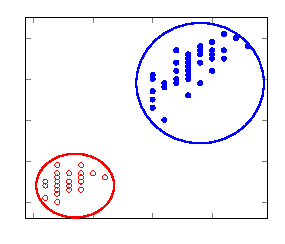
\includegraphics[width=0.7\linewidth,height=\textheight,keepaspectratio,alt={Hard, flat partitioning}]{chapters/../assets/figures/chapter10/fig-org-partitions.pdf}

}

\caption{\label{fig-org-partitions}Hard, flat partitioning}

\end{figure}%

Clustering helps in the organization (grouping) of information and makes
it easier to access and navigate. For example, when a student organizes
course materials in folders of subject areas, it becomes more efficient
for her to locate related materials when she needs to review them.

Clustering is also an important step toward information aggregation and
pattern recognition of data at hand. By discovering major groups and
themes, a high-level summarization and overview can be identified with
data instances representative of these groups. This can often be
integrated with interactive information visualization for graphical
representation and navigation of the data space.

We often think of clustering as \emph{hard} and \emph{flat partitioning}
-- \emph{hard} because cluster membership is concrete and every data
instance belongs to only one group and \emph{flat} because there is only
one level of clusters. Figure~\ref{fig-org-partitions} shows an example
of two flat partitions, where data belong to either one of them.
However, the result of clustering can be a more complex structure than
that.

\begin{figure}

\centering{

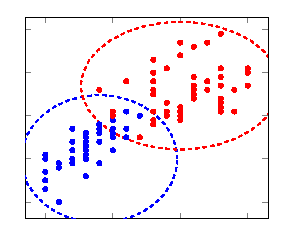
\includegraphics[width=0.7\linewidth,height=\textheight,keepaspectratio,alt={Illustration of soft partitioning, where data may belong to multiple clusters}]{chapters/../assets/figures/chapter10/fig-org-fuzzy.pdf}

}

\caption{\label{fig-org-fuzzy}Illustration of soft partitioning, where
data may belong to multiple clusters}

\end{figure}%

There are such methods for \emph{soft} or \emph{fuzzy} clustering, where
each data instance can belong to multiple clusters. For example, a book
on quantum computing can group with other books on quantum physics as
well as those in computer science/engineering. The membership is not a
concrete assignment but a degree of association. One can certainly view
such cluster associations as probabilities. Soft clustering can be very
helpful in applications where one may need different \emph{routes}, so
to speak, to data of interest.

In addition, there are clustering algorithms that produce a hierarchical
structure with levels of nested partitions, i.e.~a tree with branches
and branches of branches. Figure~\ref{fig-org-hierarchy} illustrates
hierarchical clustering, where a circle represents a cluster and a
nested circle is a child (branch) of the one containing it. This can be
achieved by either recursively merging data instances until the whole
structure has emerged (the bottom-up approach) or recursively dividing
the entire data into subsets until they can no longer be broken down
(the top-down approach).

\begin{figure}

\centering{

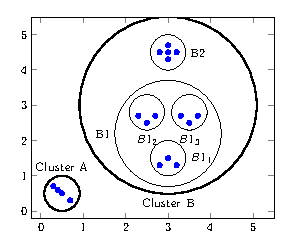
\includegraphics[width=0.7\linewidth,height=\textheight,keepaspectratio,alt={Hierarchical clustering. A nested circle represents child (branch) of the enclosing cluster.}]{chapters/../assets/figures/chapter10/fig-org-hierarchy-circles.pdf}

}

\caption{\label{fig-org-hierarchy_circles}Hierarchical clustering. A
nested circle represents child (branch) of the enclosing cluster.}

\end{figure}%

The result of hierarchical clustering in
Figure~\ref{fig-org-hierarchy_circles} can also be represented as a tree
structure in Figure~\ref{fig-org-hierarchy}. A hierarchy or dendrogram
thus constructed may reveal the underlying taxonomy of themes in the
data. It is a great tool for information organization and data
exploration.

\begin{figure}

\centering{

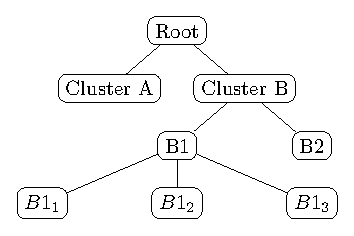
\includegraphics[width=0.7\linewidth,height=\textheight,keepaspectratio,alt={Tree representation of the hierarchical structure in the referenced figure}]{chapters/../assets/figures/chapter10/fig-org-hierarchy.pdf}

}

\caption{\label{fig-org-hierarchy}Tree representation of the
hierarchical structure in the referenced figure}

\end{figure}%

\section{Example Data}\label{example-data}

Now that we have had an overview of what clustering does and what it can
produce, we shall examine how related algorithms perform clustering on
data. We will look at a few classic methods and illustrate the
clustering process with a well-known dataset, namely the IRIS flower
data created by British statistician and geneticist Ronald Fisher. Table
shows a small sample of the data set:

\protect\phantomsection\label{tab-org-iris}
\begin{longtable}[]{@{}ccccl@{}}
\caption{IRIS flowers sample data}\tabularnewline
\toprule\noalign{}
\endfirsthead
\endhead
\bottomrule\noalign{}
\endlastfoot
Sepal & Sepal & Petal & Petal & \\
Length & Width & Length & Width & Class \\
5.1 & 3.5 & 1.4 & 0.2 & Setosa \\
7.0 & 3.2 & 4.7 & 1.4 & Versicolor \\
6.3 & 3.3 & 6.0 & 2.5 & Virginica \\
.. & .. & .. & .. & .. \\
\end{longtable}

\protect\phantomsection\label{tab-org-iris}{}

Each instance is an Iris flower observation, with measurements of its
sepal length, sepal width, petal length, and petal width in centimeters,
as well as classification of three Iris species (setosa, versicolor, or
virginica). For demonstration, we use only \(5\) data instances from
each species (\(15\) total) and focus on two variables in the analysis,
namely \emph{petal length} vs.~\emph{petal width}. In
Figure~\ref{fig-org-iris}, we plot \emph{petal length} vs.~\emph{petal
width} and color code data in each class (species).

\begin{figure}

\centering{

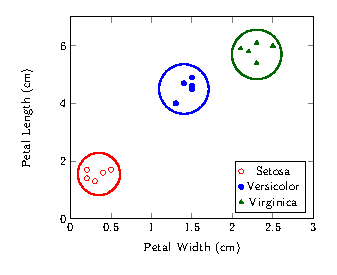
\includegraphics[width=0.7\linewidth,height=\textheight,keepaspectratio,alt={IRIS flowers data: Petal Length vs. Petal Width}]{chapters/../assets/figures/chapter10/fig-org-iris.pdf}

}

\caption{\label{fig-org-iris}IRIS flowers data: Petal Length vs.~Petal
Width}

\end{figure}%

There appear to be three clusters, as shown in
Figure~\ref{fig-org-iris}, consistent with the three species. But how
can we design algorithms to identify these clusters? Bear in mind that
any clustering method, as unsupervised learning, should be data driven
and should aim to discover inherent patterns from rather than imposing a
structure on the data.

Although clustering does not predict on the class label, we will use the
classes of the IRIS data to help evaluate (at least visually) how well a
clustering method has performed. In the end, if each identified cluster
can be related to one of the species, then the clustering process must
have done something right with regard to the data.

\section{Hierarchical Clustering}\label{hierarchical-clustering}

Hierarchical clustering is primarily used to create a tree structure of
the data. Nonetheless, one can cut the tree at a specific level to
obtain a desired number of clusters. As we discussed, there are two ways
to construct a hierarchical structure: 1) the top-down divisive approach
and 2) the bottom-up approach. We will first discuss a classic bottom-up
method, namely Hierarchical Agglomerative Clustering (HAC), and come
back to the top-down approach in the next section on .

In the bottom up approach, we start with each data instance as a
separate cluster and repeatedly merge the closest pair of clusters.
Given \(N\) instances, the initial number of clusters will be \(N\) and
this number will be reduced by \(1\) whenever two clusters are joined
together as one. The process will continue until the number of clusters
have been reduced to a (predefined) desired number \(k\) , or, if the
objective is to build the entire hierarchical structure, until all
clusters have been merged into one (the root).

This process is simple but we should clarify on two aspects before a
demonstration with the IRIS data. First, how do we measure distances in
order to determine which two are the \emph{closest}? There are many
distance and similarity functions one can use. Among others, we discuss
the Euclidean distance as a commonly used measure in Chapter~ and cosine
similarity for text analysis in
Chapter~\hyperref[ch-text]{{[}ch-text{]}}. One should carefully evaluate
how suitable a measure is with the data before adopting it.

Second, when two clusters are merged to become one, how do we represent
the new cluster so that we can measure its distance (or similarity) to
other clusters? A basic strategy is to compute the centroid of the new
cluster using vector values of member data instances. And this is the
strategy that we will use in the following demonstration as it is easy
to visualize. We will discuss several other strategies after that.

\begin{figure}

\centering{

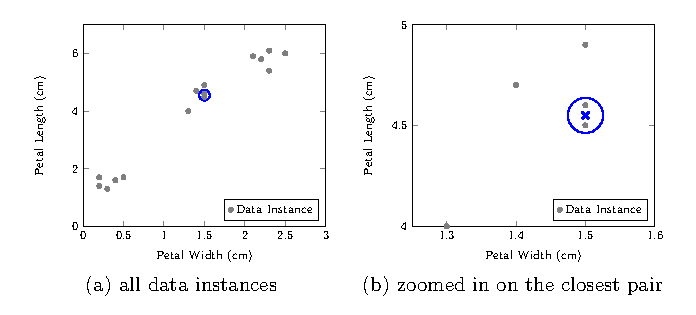
\includegraphics[width=0.7\linewidth,height=\textheight,keepaspectratio,alt={Step 1 of HAC clustering on IRIS data. The circle indicates a new cluster formed by the closest pair of instances. The centroid of the cluster is marked in (b).}]{chapters/../assets/figures/chapter10/fig-org-hac1.pdf}

}

\caption{\label{fig-org-hac1}Step \(1\) of HAC clustering on IRIS data.
The circle indicates a new cluster formed by the closest pair of
instances. The centroid of the cluster is marked \(\times\) in (b).}

\end{figure}%

Figure~\ref{fig-org-hac1} (a) plots the IRIS data and visualizes the
\(1^{st}\) step of HAC clustering. Using Euclidean distance, the closest
pair of instances can be identified, as circled on the plot, and joined
as a new cluster.

Figure~\ref{fig-org-hac1} (b) offers a closer look at the new cluster.
Once the new cluster is formed, it is represented by the average values
of its members, i.e.~the geometric center of the two data instances on
the plot (see \(\times\) in the circled cluster). Now this new cluster
with a centroid at \(\times\) is simply treated as another data instance
that can be compared to and merged with others.

Now we can continue to find the next closest pairs. In
Figure~\ref{fig-org-hac2} (a), the \(1^{st}\) merged cluster is found to
be closest to yet another data instance, and they are joined to form a
new cluster again. This continues to merge with another instance, as
shown in Figure~\ref{fig-org-hac2} (b).

\begin{figure}

\centering{

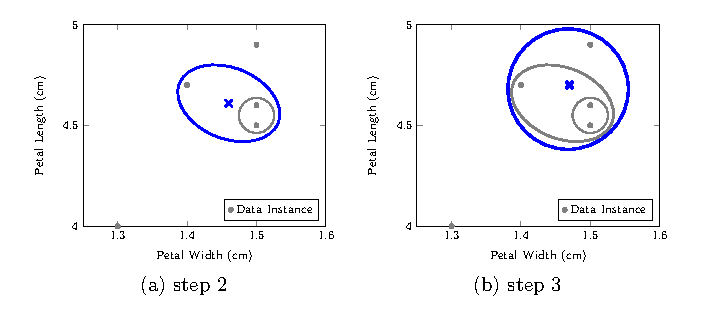
\includegraphics[width=0.7\linewidth,height=\textheight,keepaspectratio,alt={Further iterations of HAC clustering on IRIS data}]{chapters/../assets/figures/chapter10/fig-org-hac2.pdf}

}

\caption{\label{fig-org-hac2}Further iterations of HAC clustering on
IRIS data}

\end{figure}%

Repeat the merging process, we can get results in
Figure~\ref{fig-org-hac3}. If the desired number of clusters \(k\) is
predefined, one can stop the iterative process once \(k\) clusters have
been obtained. In Figure~\ref{fig-org-hac3} (a), for example, the
clustering process stops at \(3\) clusters (\(k=3\)). If one desires to
build the entire hierarchy of the data, as Figure~\ref{fig-org-hac3} (b)
shows, the process can continue until all clusters have been merged into
the root (\(k=1\)).

\begin{figure}

\centering{

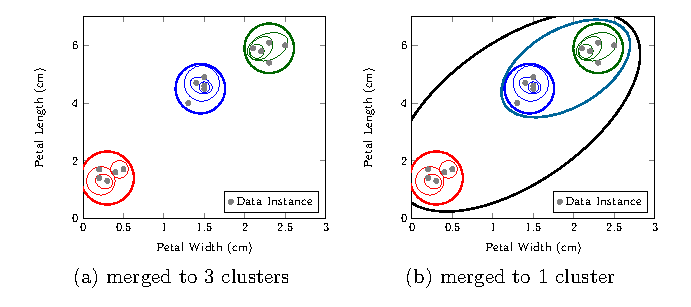
\includegraphics[width=0.7\linewidth,height=\textheight,keepaspectratio,alt={Result of HAC clustering on IRIS data}]{chapters/../assets/figures/chapter10/fig-org-hac3.pdf}

}

\caption{\label{fig-org-hac3}Result of HAC clustering on IRIS data}

\end{figure}%

\subsection{Issues of HAC}\label{issues-of-hac}

In the above demonstration, we have relied on the notion of
\emph{centroid} (with average values of cluster members) when we compute
the distance between clusters. Regardless of the distance or similarity
function being used, there are several alternative strategies for
measuring intra-cluster distances or similarities.

\emph{Average link}, for example, compare each data instance in one
cluster to another instance in the other cluster, and computes the
average distance (or similarity) of all pair-wise distances.

\emph{Single link} does the same pair-wise comparisons between members
of two clusters, but singles out the closest or most similar pair. The
shortest distance (or the greatest similarity) is then used as the
distance (or similarity) of the two clusters. \emph{Complete link}, on
the other hand, identifies the farthest pair and uses the greatest
distance (or the least similarity) as the distance (or similarity) of
the two clusters.

Hierarchical Agglomerative Clustering (HAC) is not an efficient method
and does not scale well with large data sets. Consider the amount of
computation during each iteration of HAC. Given \(N\) data instances --
which will later include merged clusters as pseudo-instances -- it
requires \(N\times(N-1)/2\) pair-wise comparison to identify the closest
pair, which is \(O(N^2)\) complexity. When we factor in the number of
iterations, which is proportional to \(\log_2{N}\) as each iteration
reduces two clusters into one, the time complexity of the entire process
is of \(O(N^2 \log{N})\).

Suppose we can manage to perform HAC on \(N=1000\) data instances, say
in \(1\) minute. For \(N=10^6\) data instances, it will take
\((\frac{10^6}{10^3})^2 \log \frac{10^6}{10^3} \approx 10,000,000\)
minutes (about \(19\) years). On large volumes of data, HAC can be
costly to perform and one has to find an alternative to hierarchical
clustering in a cost-effective way.

\section{K-means Partitioning}\label{sect:org:kmeans}

We shall now look at \emph{k-means}, a more efficient method for flat
partitioning but, as we will discuss later, can also be used for
hierarchical clustering as well. In the nutshell, k-means is a cluster
optimization technique that improves on initial (random) clusters
through iterations of cluster membership assignment and adjustment.

In the beginning when clusters are unknown, it picks a number of random
cluster centroids and assigns every data instance to a centroid
depending on its proximity (similarity). Once all cluster membership has
been determined, the centroid (center) of each cluster can be
re-computed based on its assigned member instances. With the re-computed
centroids, data instances will be reassigned, which will lead to further
change of cluster centroids. So the process will continue on with
centroid adjustment and cluster membership re-assignment, until the
centroids no longer move (or move very little) or it has gone through a
sufficient number of iterations.

Now let's look at how k-means may identify clusters from the IRIS data.
Again, we set the number of desired clusters \(k=3\) to see whether it
may produce clusters consistent with the three Iris species.

\begin{figure}

\centering{

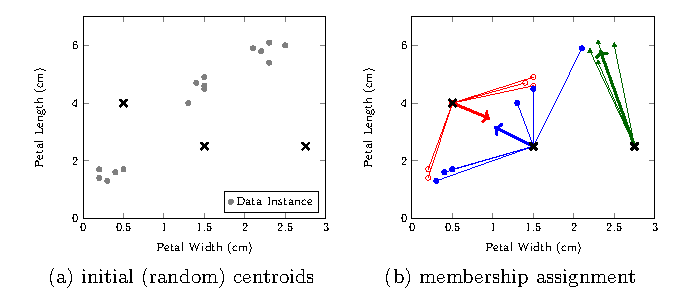
\includegraphics[width=0.7\linewidth,height=\textheight,keepaspectratio,alt={K-means initial steps. A represents an initial centroid. Undirected lines represent cluster membership. Directed lines indicates how the centroid will move (change) after re-computation based on assigned members.}]{chapters/../assets/figures/chapter10/fig-org-kmeans1.pdf}

}

\caption{\label{fig-org-kmeans1}K-means initial steps. A \(\times\)
represents an initial centroid. Undirected lines represent cluster
membership. Directed lines \(\nearrow\) indicates how the centroid will
move (change) after re-computation based on assigned members.}

\end{figure}%

With data plotted in Figure~\ref{fig-org-kmeans1} (a), we start with
\(3\) random cluster centroids, shown as \(\times\) in the plot. For
each data instance, we compute its distance to each of the three initial
centroids and identify the closest centroid, to which it will be
assigned as a member. Figure~\ref{fig-org-kmeans1} (b) shows lines
connecting data instances to their corresponding closest centroids.

Once membership of each cluster is assigned, the center of cluster can
be re-computed based on averaging member instances. After this
computation, the centroids will likely change (move). Directed lines
(arrows) in Figure~\ref{fig-org-kmeans1} (b) represent the changes of
cluster centroids.

\begin{figure}

\centering{

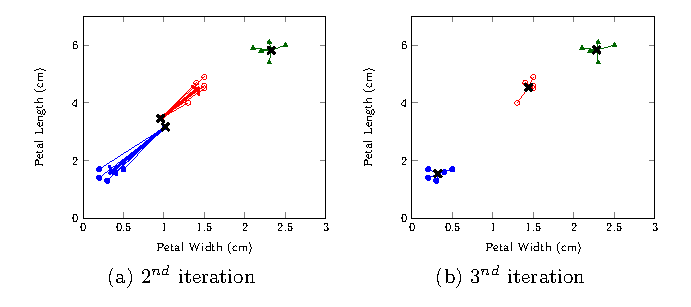
\includegraphics[width=0.7\linewidth,height=\textheight,keepaspectratio,alt={K-means further steps. A represents an centroid before it is updated. Undirected lines represent cluster membership. Directed lines indicates how the centroid will move (change) after re-computation based on assigned members.}]{chapters/../assets/figures/chapter10/fig-org-kmeans2.pdf}

}

\caption{\label{fig-org-kmeans2}K-means further steps. A \(\times\)
represents an centroid before it is updated. Undirected lines represent
cluster membership. Directed lines \(\nearrow\) indicates how the
centroid will move (change) after re-computation based on assigned
members.}

\end{figure}%

With the new cluster centroids, the distance of each data instance has
also changed and should be measured again to find out which cluster one
belongs to now. By doing so, some data instances may move from one
cluster to another, as shown in the \(2^{nd}\) iteration in
Figure~\ref{fig-org-kmeans2} (a), which, in turn, leads to further
changes of cluster centroids. See the \(3^{rd}\) iteration in
Figure~\ref{fig-org-kmeans2} (b). By repeating the iterations of cluster
member assignment and centroid re-computation, the cluster centroids
will continue to move and gradually converge. One may stop the k-means
optimization process when cluster centroid does not move or moves very
little, or after a certain number of iterations.

\begin{figure}

\centering{

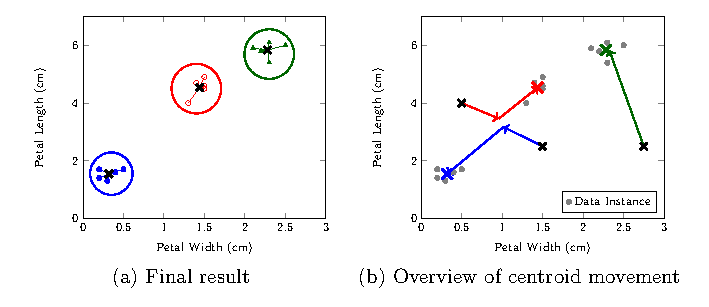
\includegraphics[width=0.7\linewidth,height=\textheight,keepaspectratio,alt={K-means final clusters and steps}]{chapters/../assets/figures/chapter10/fig-org-kmeans3.pdf}

}

\caption{\label{fig-org-kmeans3}K-means final clusters and steps}

\end{figure}%

For the small IRIS data set here, it only takes less than \(5\)
iterations for the cluster centroids to converge (with little further
movement). Figure~\ref{fig-org-kmeans3} (a) shows the final \(3\)
clusters thus identified and they are consistent with the three species
of Iris flowers in the data. Figure~\ref{fig-org-kmeans3} (b) gives an
overview of the movement of cluster centroids through the iterations.
Even though we started with random centroids, k-means gradually moves
the centroids toward more representative segments of the data and, in
the end, reaches an optimal outcome.

\subsection{Issues of K-means}\label{issues-of-k-means}

K-means can be interpreted as to minimize member instances' mean squared
distance from their centroid. The iterative process can always converge
to an optimum, but there is no guarantee that it will be globally
optimal. In each iteration, it compares \(k\) clusters to \(N\) data
instances, which is \(O(kN)\). Because \(k\) is usually much smaller
than \(N\), k-means is much more efficient and scalable than HAC.

Clustering is understood as unsupervised learning. Theoretically, it is
data driven without human input. In practice, however, it is not a clear
cut. There are many ways in which one can influence the outcome of
clustering, making it somewhat supervised. With the k-means method, for
example, one has to predefine the number of clusters to be generated,
which makes the outcome rather arbitrary. The data at hand does not
necessarily have that supposed \(k\) number of clusters. One may have to
test and evaluate clustering with different numbers of clusters to find
out what an ideal \(k\) may be.

The distance function also plays an important role in clustering. For
text clustering, feature (term) distributions matter more than the
absolute weights of terms. In that domain of applications, cosine
(angle) similarity works better than Euclidean distance and like
measures. Furthermore, even with the same distance function, the weights
and scales of variables (features) make a major difference. If all
variables are to be treated equally, then they should be normalized to
the same scale, e.g.~within \([0,1]\) for positive values. Otherwise,
they should be properly weighted by their discriminative power based on
domain theory and/or statistics.

\section{Probabilistic Clustering}\label{probabilistic-clustering}

While k-means discovers cluster centroids, the Euclidean distance, for
example, essentially defines a cluster boundary as a sphere of a certain
radius in a dimensional space, e.g.~circles on two dimensions in
Figure~\ref{fig-org-kmeans3} (a). This implies two basic assumptions: 1)
the distribution of member instances in a cluster is spherical, and 2)
each data instance only belongs to one and only one cluster.

Is it possible to assume a different data distribution for clustering?
In the same time, can there be soft (fuzzy) associations between data
instances and clusters? The soft cluster membership can perhaps be
thought of as probabilities.

Indeed, there is a general probabilistic approach to clustering, namely
a model-based clustering. The term \emph{model} means that data are
assumed to follow a distribution function with certain parameters
(model) to be discovered. So based on the model, one can estimate the
probabilities of cluster membership and try to maximize the
probabilities in the process of identifying the clusters.

For simpler illustration and explanation, let's first consider only one
variable, \emph{petal width}, in the IRIS data. Suppose data instances
with petal width values \(v\) follows the normal distribution, based on
which, as we discussed in Chapter~, the probability density of value
\(v\) is computed by:

\[\begin{aligned}
  f(v)
  & = & f(v|\mu,\delta^2) \\
  & = & \frac{1}{\sqrt{2\pi\delta^2}} e^{-\frac{(v-\mu)^2}{2\delta^2}}
\end{aligned}\]

In the context of clustering, however, we assume the same normal
distribution \emph{within} each cluster \(c\). The above density
function can be extended to include terms related to the cluster \(c\)
and the probability of a value \(v\) in cluster \(c\) can bey computed
by:

\[\begin{aligned}
  P(v|c)
  & \propto & f_{c}(v) \\
  & = & f(v|\mu_c,\delta_c^2) \\
  & = & \frac{1}{\sqrt{2\pi\delta_c^2}} e^{-\frac{(v-\mu_c)^2}{2\delta_c^2}}
\end{aligned}\]

where \(\mu_c\) and \(\delta_c^2\) are the mean and variance of values
associated with cluster \(c\), the only two parameters of the model for
each cluster.

The above formula shows that, in order to compute related probabilities,
we need to know parameter values, namely mean \(\mu_c\) and variance
\(\delta_c^2\), for each cluster \(c\). The problem is, we are yet to
identify these values, which, in fact, are based on related
probabilities.

With the chicken or the egg dilemma, we shall start with some initial
values for the \(\mu_c\) and \(\delta_c^2\) so that we can feed them
into the calculation of probabilities, which then help in the
identification of better \(\mu_c\) and \(\delta_c^2\) values. This is
similar to k-means where we start with initial centroids, which, through
membership assignment and reassignment, change and improve.

\subsection{Initialization}\label{initialization}

With the IRIS data on only one dimension, i.e.~petal width, we randomize
\(\mu_c\) and \(\delta_c\) for \(k=3\) clusters: \(\mu_1=1\) and
\(\delta_1=0.25\) for cluster \(c_1\), \(\mu_2=1.6\) and
\(\delta_2=0.25\) for cluster \(c_2\), and \(\mu_3=2.8\) and
\(\delta_1=0.25\) for cluster \(c_3\). Figure~\ref{fig-org-em1} shows
the distribution of IRIS data instances on the petal width \(v\)
dimension, with a normal (bell) curve based on each set of initial
parameters.

\begin{figure}

\centering{

\includegraphics[width=0.7\linewidth,height=\textheight,keepaspectratio,alt={Initial parameters of normal distributions. are IRIS data instances. marks each an initial (random) mean (similar to a centroid), around which a normal distribution curve is plotted. The shaded area under curve shows the range of deviation from mean, i.e. {[}-, +{]}.}]{chapters/../assets/figures/chapter10/fig-org-em1.pdf}

}

\caption{\label{fig-org-em1}Initial parameters of normal distributions.
\(\circ\) are IRIS data instances. \(\times\) marks each an initial
(random) mean \(\mu\) (similar to a centroid), around which a normal
distribution curve is plotted. The shaded area under curve shows the
range of deviation from mean, i.e.~\([\mu-\delta, \mu+\delta]\).}

\end{figure}%

In addition, we don't know the prior probability \(P(c)\) of each
cluster \(c\). If we assume equal chances, we have for the \(3\)
clusters in the IRIS data: \(P(c_1)=P(c_2)=P(c_3)=1/3\).

\subsection{Expectation}\label{expectation}

Given each cluster model with the initial parameter, we can estimate
\(P(v|c)\), how likely an instance \(v\) can be observed -- generated
from the model -- in that cluster \(c\).

For now, however, we are more interested in finding the probability of
an instance's membership association with a cluster. That is, given an
instance \(v\), how likely it is associated with each cluster \(c\),
\(P(c|v)\). Following the Bayes Theorem, \(P(c|v)\) can be estimated
using \(P(v|c)\):

\[\begin{aligned}
  P(c|v)
  & = & \frac{P(v|c) P(c)}{P(v)}  \\
  & = & \frac{f(v|\mu_c,\delta_c^2) P(c)}{\sum_{i=1}^{k} P(c_i) f(v|\mu_{c_i},\delta_{c_i}^2)}
\end{aligned}\]

where \(k\) is the number of clusters and the denominator is the sum of
probabilities for the data instance \(v\) to be generated by
distribution models of all \(k\) clusters.

Computing \(P(c|v)\) is similar to the membership assignment of data
instances to clusters in k-means. But instead of a \emph{hard}
membership, we have a probabilistic (soft) assignment here. We refer to
the process of estimating the posterior probabilities of cluster
membership as \emph{Expectation}.

Let's apply this to the IRIS data. We use the first data instance with
petal width \(v=0.2\) (cm) (see the \(\circ\) closest to the zero in
Figure~\ref{fig-org-em1}). First, we compute \(P(v|c)\), probability
that each cluster model will generate the instance \(v=0.2\):

\[\begin{aligned}
  P(v=0.2|c_1)
  & \propto & f_{c_1}(v=0.2) \\
  & = & f(v=0.2|\mu_1=1,\delta_1=0.25) \\
  & = & \frac{1}{\sqrt{2\times0.25^2 \pi}} e^{-\frac{(0.2-1)^2}{2\times0.25^2}} \\
  & = & 0.00954 \\
  P(v=0.2|c_2) & \propto &  2.5 \times 10^{-7} \\
  P(v=0.2|c_3) & \propto &  5.2 \times 10^{-24} \\
\end{aligned}\]

As you can see from the Figure~\ref{fig-org-em1}, \(v=0.2\) is on the
far left side of the first (red) bell curve centered on \(1\), and has a
very small probability density \(P(v=0.2|c_1) \propto 0.00954\). This is
further remove from the centers of the second (blue) and third (green)
normal curves, and probability densities corresponding to \(c_2\) and
\(c_3\) are much smaller.

With these values, we can now compute \(P(v)\), which is the weighted
sum of probabilities that the \(3\) cluster models will generate data
\(v=0.2\):

\[\begin{aligned}
  P(v=0.2)
  & = & \sum_{i=1}^{3} P(c_i) f(v=0.2|\mu_{c_i},\delta_{c_i}^2) \\
  & = & 1/3 \times 0.00954 + 1/3 \times 2.5 \times 10^{-7} + 1/3 \times 5.2 \times 10^{-24} \\
  & = & 0.00318
\end{aligned}\]

Plug these values into Equation~\hyperref[eq-org-pcv]{{[}eq-org-pcv{]}},
we can compute the probability of data instance \(v=0.2\) belonging to
each cluster for the \emph{Expectation} step:

\[\begin{aligned}
  P(c_1|v=0.2)
  & = & \frac{P(v=0.2|c_1) P(c_1)}{P(v=0.2)} \\
  % & = & \frac{f(v|\mu_{c_1},\delta_{c_1}^2) P(c_1)}{\sum_{i=1}^{3} P(c_i) f(v|\mu_{c_i},\delta_{c_i}^2)} \\
  & = & \frac{0.00954 \times 1/3}{0.00318} \\
  & \approx & 1 \\
  P(c_2|v=0.2) & = & 2.59 \times 10^{-5} \\
  P(c_3|v=0.2) & = & 5.46 \times 10^{-22}
\end{aligned}\]

Apparently, data instance \(v=0.2\) is much more likely to belong to the
cluster \(c_1\) (the red bell curve on the left) than to the other
clusters, which are far away away as shown in Figure~\ref{fig-org-em1}.

Now that we have identified the membership probabilities for the first
instance, we shall continue to do the same for all other data instances
(\(N=15\) for the IRIS data) and conclude the \emph{Expectation} step
with all probabilistic membership "assignment." For example, here are
related probabilities for two more data instances in IRIS: \(v=0.4\)
(\(2^{nd}\) instance) and \(v=2.3\) (\(15^{th}\) instance).

\[\begin{aligned}
  P(c_1|v=0.4) & \approx & 1 \\
  P(c_2|v=0.4) & = & 0.000177 \\
  P(c_3|v=0.4) & = & 1.7 \times 10^{-19} \\
  P(c_1|v=1.3) & = & 8.66 \times 10^{-6} \\
  P(c_2|v=1.3) & = & 0.128 \\
  P(c_3|v=1.3) & = & 0.872
\end{aligned}\]

\begin{figure}

\centering{

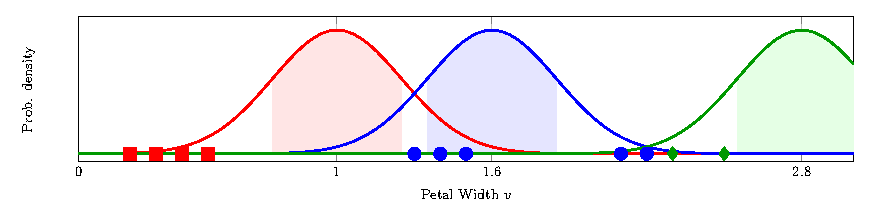
\includegraphics[width=0.7\linewidth,height=\textheight,keepaspectratio,alt={First expectation result. Color of a data instance indicates the cluster membership with the highest probability.}]{chapters/../assets/figures/chapter10/fig-org-em2.pdf}

}

\caption{\label{fig-org-em2}First expectation result. Color of a data
instance indicates the cluster membership with the highest probability.}

\end{figure}%

Figure~\ref{fig-org-em2} shows the color-coded result of the first
\emph{Expectation} step on the IRIS data. A data instance's color
indicates the cluster with the highest probability -- that is, the bell
curve that best "covers" the data instance.

\subsection{Maximization}\label{maximization}

The objective of clustering is to find clusters such that the overall
probability of observed data instances is maximized. That is to maximize
the joint probability for all data instances, which is the product of
all \(P(v|c)\) if we assume statistical independence:

\[\begin{aligned}
  \mathop{\mathrm{arg\,max}}_{\theta_c} \prod_v P(v|c)
\end{aligned}\]

where \(\theta\) are parameters of the distribution models and, with the
normal distribution assumption, are \(\mu\) and \(\delta^2\) of each
cluster distribution. This is equivalent to maximizing the
log-likelihood:

\[\begin{aligned}
    \log \prod_v P(v|c)
    & = & \log \prod_v f(v|\mu_c,\delta_c^2) \\
    & = & \sum_v \log f(v|\mu_c,\delta_c^2)
\end{aligned}\]

The parameters can be estimated by:

\[\begin{aligned}
  \hat{\mu_c} & = & \frac{\sum_v v P(c|v)}{\sum_v P(c|v)} \\
  \hat{\delta_c^2} & = & \frac{\sum_v (v - \hat{\mu_c})^2 P(c|v)}{\sum_v P(c|v)}
\end{aligned}\]

where \(v\) is each one of \(N\) data instances (\(N=15\) in the small
IRIS data subset here) and \(P(c|v)\) is the probability that \(v\) is
associated with cluster \(c\).

It turns out that there is not a simple direct solution to maximizing
the log-likelihood. However, if we look at the result from the
\emph{Expectation} step, there is a way in which we can maximize this by
following the data and improving the \emph{representative} of the
cluster models, similar to how k-means iterates.

Now that data instances have been assigned, probabilistically, to each
cluster, the original model for each cluster is no longer representative
of data associated with them. In Figure~\ref{fig-org-em2}, for example,
the first (red) bell curve is not centered on the data instances most
highly associated with it.

This is similar to k-means where the original centroid does no longer
represent the center of member instances. And the models -- with
parameters mean \(\mu_c\) and variance \(\delta_c^2\) for each cluster
\(c\) -- will have to be recomputed. This re-computation of parameters,
in the context of model-based clustering, is the \emph{Maximization}
step.

Now back to the IRIS data. With the assigned posterior probabilities
\(P(c|v)\), we can now update the mean and variance for each cluster
model. For cluster \(c_1\) and \(N=15\) data instances, we have:

\[\begin{aligned}
  \hat{\mu_1}
  & = & \frac{\sum_v v P(c_1|v)}{\sum_v P(c_1|v)} \\
  % & = & \frac{v_1\times P(c_1|v_1) + v_2\times P(c_1|v_2) + .. + v_{15}\times P(c_1|v_{15})}{P(c_1|v_1) + P(c_1|v_2) + .. + P(c_1|v_{15})} \\
  & = & \frac{0.2\times1 + 0.4\times1 + .. + 1.3\times8.66 \times 10^{-5}}{1+1+..+8.66 \times 10^{-5}} \\
  & = & 0.522 \\
  \hat{\delta_1}
  & = & \sqrt{ \frac{\sum_v (v - \hat{\mu_1})^2 P(c_1|v)}{\sum_v P(c_1|v)} }\\
  & = & \sqrt{ \frac{(0.2-0.522)^2\times1 + (0.4-0.522)^2\times1 + .. + (1.3-0.522)^2\times8.66 \times 10^{-5}}{1+1+..+8.66 \times 10^{-5}} }\\
  & = & 0.433
\end{aligned}\]

Likewise, we can update models for cluster \(c_2\) with
\(\hat{\mu_2}=1.67\) and \(\hat{\delta_2}=0.332\), and cluster \(c_3\)
with \(\hat{\mu_3}=2.34\) and \(\hat{\delta_3}=0.116\).

\begin{figure}

\centering{

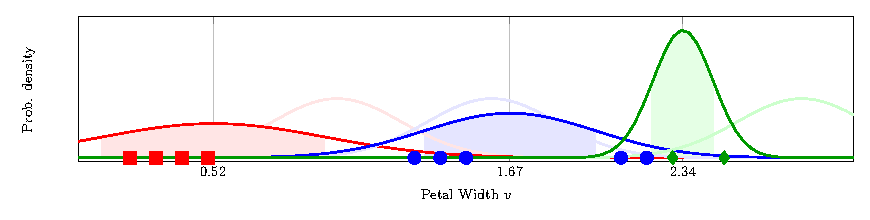
\includegraphics[width=0.7\linewidth,height=\textheight,keepaspectratio,alt={First Maximization result. A bell curve with with a shaded area ( delta) is the new model with updated parameters for the cluster.}]{chapters/../assets/figures/chapter10/fig-org-em3.pdf}

}

\caption{\label{fig-org-em3}First Maximization result. A bell curve with
with a shaded area (\(\pm delta\)) is the new model with updated
parameters for the cluster.}

\end{figure}%

Figure~\ref{fig-org-em3} shows the result of this \emph{Maximization}
step. The models (normal curves) have moved closer to their more highly
associated data instances. This is very similar to re-computation of
centroids -- thus causing them to move -- in k-means clustering. With
Maximization, more than one parameters are needed to specify a model.
For normal distribution models, both mean \(\mu\) and variance
\(\delta^2\) are to be updated. If one assumes a different probability
distribution, then a different set of parameters will be maximized.

\subsection{Iterations of
Expection-Maximization}\label{iterations-of-expection-maximization}

Now that the cluster models have changed, we need to go back to the
\emph{Expectation} step and re-compute the posterior probabilities
\(P(c|v)\). Once the probabilities are changed, the model parameters
will be updated again in the next \emph{Maximization} step. The process
of Expectation-Maximization will repeat itself until the models no
longer changed, where the overall probability of models generating
observed data instances has been maximized.

Figure~\ref{fig-org-em4} shows further iterations of EM on the IRIS
data. Visually, the cluster models (curves) move increasingly closer to
the data instances they represent and, in the end, get well aligned with
them.

\begin{figure}

\centering{

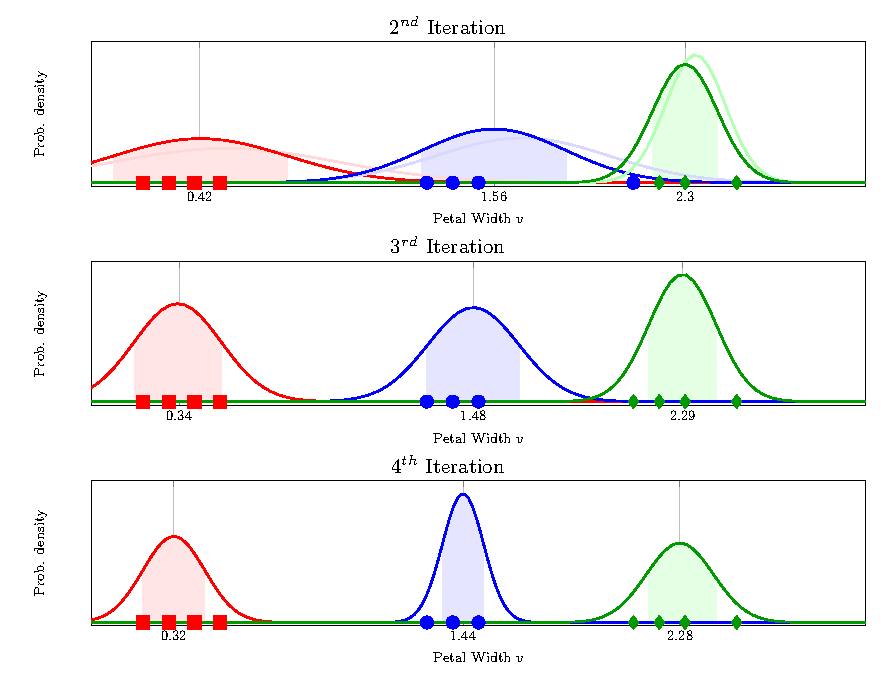
\includegraphics[width=0.7\linewidth,height=\textheight,keepaspectratio,alt={Iterations of Expectation and Maximization. Note that there are 5 data instances in each iris species. But because their petal width values overlap on the only dimension, there appear to be 3 or 4 instances in each cluster, which, in fact, has 5.}]{chapters/../assets/figures/chapter10/fig-org-em4.pdf}

}

\caption{\label{fig-org-em4}Iterations of Expectation and Maximization.
Note that there are \(5\) data instances in each iris species. But
because their petal width values overlap on the only dimension, there
appear to be \(3\) or \(4\) instances in each cluster, which, in fact,
has \(5\).}

\end{figure}%

\subsection{EM with Higher
Dimensionality}\label{em-with-higher-dimensionality}

Our discussion has been focused on the it Expectation-Maximization
method on one dimension with the univariate normal distribution. In
real-world applications, however, there is hardly any clustering problem
that can be resolved with this simplified version.

Normally EM has to take into account multiple, if not thousdands or even
millions of, variables. Instead of univariate distributions, one will
have to rely on multivariate distributions. For example, rather than
using univariate normal distributions with means and variances, one will
instead rely on co-variances in a mixture Gaussian model.

In addition, the normal (Gaussian) distribution is only one of many
distribution functions that can be used with EM clustering. In text
clustering application, for example, it is very common to use poisson
distributions. Regardless of the assumed distribution, the idea and
process of expectation and maximization for the optimization of
log-likelihood of observed data remain the same.

\part{Language, Retrieval, and Structure}

\chapter{Text and Human Language}\label{ch-text}

The big print giveth, and the fine print taketh away.

\emph{Fulton J. Sheen}

Text has been the primary form of documentation in human history. Today
large volumes of unstructured text data are being generated and
disseminated at an unprecedented pace, via such media as tweets, emails,
and scholarly publications. The magnitude of these data has far exceeded
our human capacity to read and digest. How can we possibly sift through
the world of written text and access what we need? In what ways can
computers, which have helped create this ever-growing pile of data, be
harnessed to also help us discover relevance and meaning?

\section{Text Vectorization}\label{text-vectorization}

Let's start with some basic issues and ideas for processing text.

Imagine having a long legal document, it can be stored digitally along
with other documents and files. In its raw text format, you can hardly
use the document to compute and compare -- for example, to find other
documents related to the same or similar cases -- unless we can convert
the text into some numbers to be used in the calculation.

Indeed, the first step of text processing involves a general process
called \emph{vectorization}, which identifies elements in the text and
assigns numbers (weights) to them as its numerical representation. The
result of this is a list of values, which can then be used for
searching, ranking, and association.

\subsection{Tokenization}\label{tokenization}

Through \emph{tokenization}, the text can be split into basic elements
(tokens) such as paragraphs, sentences, phrases, and/or words. Taking
single words as basic elements, the following text:

John is quicker than Mary.

can be split into individual tokens \emph{John}, \emph{is},
\emph{quicker}, \emph{than}, and \emph{Mary}. In a simple classic
approach, we only try to capture what tokens (keywords) occur in the
text and pay no heed to the order in which they appear. This is referred
to as the \emph{bag of words} model, which will lead to some loss of
information. Apparently, with this treatment, tokenization of the above
text will result in the identical \emph{bag of words} with the
following:

Mary is quicker than John.

where the only difference is the order and the meaning is simply the
opposite. Indeed, for analyses where the semantic interpretation of a
text is critical, the model will suffer from the loss of order. In many
practical applications, nonetheless, the \emph{bag of words} works
sufficiently well where the central problem is about finding
associations through the keywords. For now, we stick with this basic
model and revisit the issue of word order later.

Now that we identify the tokens (words), one may consider normalize them
so that the same word types in various forms can be unified and treated
as the same. In English, one can apply normalization techniques such as:

\begin{itemize}
\item
  \emph{Case folding}, which changes all tokens into lower-case,
  e.g.~\emph{John} and \emph{JOHN} \(\to\) \emph{john};
\item
  \emph{Stemming}, which reduces tokens to their \emph{roots},
  e.g.~\emph{compression} and \emph{compressed} \(\to\) \emph{compress};
\item
  \emph{Lemmatization}, which converts word variants to their base form,
  e.g. \emph{are} and \emph{is} \(\to\) \emph{be};
\end{itemize}

These techniques are language and domain-dependent. Aside from potential
benefits of unifying tokens of the same type, token normalization may
also lead to undesired consequences, e.g.~to treat \emph{CAT} (the
company) and \emph{cat} as the same. So careful examination of data and
application is necessary to determine whether related normalization
techniques may be instrumental or detrimental.

Also, note that tokens are not limited to single words. One can use a
moving window to take two, three, or more consecutive words at a time to
identify all possible phrases or n-grams. Likewise, you can use a moving
window to identify any \(n\) consecutive characters as tokens. Character
n-grams have shown its utility in applications such as spam detection,
where junk emails may pad normal keywords with special characters to
avoid being identified.

\subsection{Term Weighting}\label{fig-text-weight}

Once tokens -- single words or phrases -- have been identified, they can
be sorted and merged into a set of unique tokens, which we refer to as
the \emph{dictionary}. Suppose we have a book collection of \emph{The
Chronicles of Narnia}, for which we only store their titles\footnote{Bear
  in mind that full-text is often considered and analyzed in real-world
  text data. We use the title only here for the simplicity of
  illustration.}:

\begin{enumerate}
\def\labelenumi{\arabic{enumi}.}
\item
  The Lion, the Witch and the Wardrobe
\item
  The Voyage of the Dawn Treader
\item
  The Horse and His Boy
\end{enumerate}

Based on tokenization of single words with case-folding, the following
dictionary (alphabetically ordered) can be identified from this small
collection:

{\def\LTcaptype{none} % do not increment counter
\begin{longtable}[]{@{}cccccccccccl@{}}
\toprule\noalign{}
1 & 2 & 3 & 4 & 5 & 6 & 7 & 8 & 9 & 10 & 11 & \\
\midrule\noalign{}
\endhead
\bottomrule\noalign{}
\endlastfoot
and & boy & dawn & his & horse & lion & the & treader & voyage &
wardrobe & witch & \\
\end{longtable}
}

Now we can use terms in this dictionary to represent each document based
on their occurrences, \(0\) if one does not occur and \(1\) if it does.
The following matrix shows such a \emph{binary representation}:

{\def\LTcaptype{none} % do not increment counter
\begin{longtable}[]{@{}lccccccccccc@{}}
\toprule\noalign{}
& 1 & 2 & 3 & 4 & 5 & 6 & 7 & 8 & 9 & 10 & 11 \\
\midrule\noalign{}
\endhead
\bottomrule\noalign{}
\endlastfoot
DOC & and & boy & dawn & his & horse & lion & the & treader & voyage &
wardrobe & witch \\
1 & 1 & 0 & 0 & 0 & 0 & 1 & 1 & 0 & 0 & 1 & 1 \\
2 & 0 & 0 & 1 & 0 & 0 & 1 & 1 & 1 & 1 & 0 & 0 \\
3 & 1 & 1 & 0 & 1 & 1 & 0 & 1 & 0 & 0 & 0 & 0 \\
\end{longtable}
}

\protect\phantomsection\label{tab-text-binary}{}

The size of the dictionary will increase with the size of the text
collection and the length of each document. However, one can imagine
that, for each document, not all dictionary terms will occur and
therefore some (many in fact) of vector values are \(0\)s. A more
efficient representation is a sparse vector, where only non-zero values
(\(1\) in the binary case here) are retained. For example, document
\(3\) in the above matrix can be represented as:

{\def\LTcaptype{none} % do not increment counter
\begin{longtable}[]{@{}ccccccc@{}}
\toprule\noalign{}
( & 1 & 2 & 4 & 5 & 7 & ) \\
\midrule\noalign{}
\endhead
\bottomrule\noalign{}
\endlastfoot
& and & boy & his & horse & the & \\
\end{longtable}
}

which only includes terms that appear in the document and have \(1\)
values.

The binary representation only whether or not a term occurs. This is a
reasonable treatment for small text documents such as the above example
and tweets. With longer text documents, when full-text is used for
vectorization, it is useful to also consider \emph{term frequency} (TF).

\(TF_{dt}\) is the number of times a term \(t\) appears in document
\(d\). It is often observed that a term with a higher term frequency in
a document is more relevant to the document's topical theme and should,
therefore, be given a higher weight. One can simply use the term
frequency as term weight:

\[\begin{aligned}
  w_{dt} & = & TF_{dt}
\end{aligned}\]

One can also normalize the TF value with logarithm:

\[\begin{aligned}
  w_{dt} & = &
\begin{cases}
  1 + \log TF_{dt}, & \text{if}\ TF_{dt}>0 \\
  0, & \text{otherwise}
\end{cases}
\end{aligned}\]

A basic assumption of counting occurrences in the term frequency weight
is that all occurrences are equal and should count equally. In light of
the Zipf law, however, we know words are used unequally.

Some words appear more frequently simply because of the effect of
\emph{least effort}. Some are stop-words like \emph{a} and \emph{the}
that contribute little in meaning. For many of these, there is one thing
in common -- they appear frequently not only in the current document but
also in other documents as well.

In general, we observe that some terms are used so \emph{broadly} in so
many documents that they can hardly help differentiate one document from
another. They are too broad to be \emph{specific} and informative.

On the other extreme, some terms are used in only a very few documents
and they very clearly distinguish these documents from others. These
terms are rarer, more specific, and should be given more weight
according to the observation here.

Imagine we randomly draw a document from the entire text collection,
there is a probability that term \(t\) will appear, which can be
estimated by:

\[\begin{aligned}
  p(t|C) & = & \frac{n_t}{N} \\
  p(t'|C) & = & 1 - \frac{n_t}{N}
\end{aligned}\]

where \(n_t\) is the number of documents containing term \(t\) and \(N\)
is the total number of documents in the collection \(C\). \(p(t'|C)\) is
the complimentary probability that \(t\) does NOT occur.

For a specific document \(d\) where term \(t\) appears, it is certain so
the probability of observing the term is:

\[\begin{aligned}
  p(t|d) & = & 1 \\
  p(t'|d) & = & 0
\end{aligned}\]

The amount of \emph{information gain} or relative entropy, according to
chapter~\hyperref[ch-info]{{[}ch-info{]}}, by seeing the term in
document \(d\) out of collection \(C\), can be computed by:

\[\begin{aligned}
  Info(t)
  & = & DL[P(t|d) || P(t|C)] \\
  & = & - \sum_{x \in (t,t')} p(x|d) \log \frac{p(x|C)}{p(x|d)} \\
  & = & - p(t|d) \log \frac{p(t|C)}{p(t|d)} - p(t'|d) \log \frac{p(t'|C)}{p(t'|d)} \\
  & = & - 1 \cdot \log \frac{n_t}{N} - 0 \cdot  \log \frac{p(t'|C)}{p(t'|d)} \\
  & = & - \log \frac{n_t}{N}
\end{aligned}\]

This information gain of term \(t\) is in fact the exactly the classic
\emph{Inverse Document Frequency} (IDF) weighting scheme:

\[\begin{aligned}
  IDF_t
  & = & Info(t) \\
  & = & \frac{N}{n_t}
\end{aligned}\]

where \(n_t\), the number of documents with term \(t\), is commonly
referred to as \emph{document frequency} (DF).

IDF measures how informative a term is when it appears in a document.
For a term that appears in all documents in the collection -- the
stop-words for example -- \(n_t\) is the same as \(N\) and its IDF
weight becomes:

\[\begin{aligned}
  IDF_t & = & \log \frac{N}{N} \\
        & = & \log 1 \\
        & = & 0
\end{aligned}\]

For a term that appears in very few documents in a large collection,
\(n_t << N\) and the IDF weight is great. In this way, the IDF weight
penalizes broader terms used in many documents and rewards more
selective, rare terms.

Please note that IDF is a collection-wide statistic for each term
whereas term frequency (TF) is term statistic specific to a document.
They address two separate aspects of term weighting and are often
combined for document representation. The combined weighting scheme,
namely the classic \emph{TF*IDF}, assigns a term's weight by:

\[\begin{aligned}
w_{dt} & = & TF_{dt} \log \frac{N}{n_t}
\end{aligned}\]

or with log-transformed TF weight:

\[\begin{aligned}
w_{dt} & = &
\begin{cases}
  (1 + \log TF_{dt}) \log \frac{N}{n_t} , & \text{if}\ TF_{dt}>0 \\
  0, & \text{otherwise}
\end{cases}
\end{aligned}\]

where \(TF_{dt}\) is the number of times term \(t\) occurs in document
\(d\) (TF), \(n_t\) is the number of documents having \(t\) (DF), and
\(N\) is the total number of document in the collection.

In certain applications, TF may be normalized by document length to
alleviate potential favoritism toward longer documents. This is one of
the most widely used term weighting methods in information retrieval and
text mining.

\section{Similarity Measures}\label{fig-text-sim}

Once each document is represented as a vector of terms with weights, we
can conduct various operations, such as clustering and ranking, on them.
The basic unit of these computational tasks is to measure how similar or
dissimilar one document is to another.

A simple method to compute the similarity of any two documents \(d_u\)
and \(d_v\) is by the dot product of their vector values:

\[\begin{aligned}
Sim(d_u, d_v) & = & \sum_{t \in T}^{m} w_{ut} w_{vt}
\end{aligned}\]

where for each term \(t\) in dictionary \(T\), \(w_{u,t}\) is the weight
of \(t\) in document \(d_u\), and \(w_{v,t}\) is the weight of \(t\) in
document \(d_v\). For example, the similarity of doc \(1\) and \(3\)
given the binary matrix of
Table~\hyperref[tab-text-binary]{{[}tab-text-binary{]}} can be computed
by:

\[\begin{aligned}
Sim(d_1, d_3)
& = & 1\times1 + 0\times1 + 0\times0 + ... + 1\times0 \\
& = & 2
\end{aligned}\]

The dot product coefficient in
Equation~\hyperref[eq-text-dotp]{{[}eq-text-dotp{]}} can be used with
any term weighting schemes including TF and TF*IDF. However, this
similarity measure is not normalized by any size factor and its score
can be inflated by document lengths and favor those longer documents. A
remedy of this is the classic cosine similarity, which we will discuss
in depth.

A binary sparse vector can also be regarded as a \emph{set}, that is, a
set including all unique terms that occur in the document. Several
similarity coefficients can be computed based on sets. The \emph{Dice
Coefficient} computes the ratio between two sets' intersection size and
the mean of their sizes:

\[\begin{aligned}
Dice(d_u, d_v)
& = & \frac{|d_u \cap d_v|}{(|d_u| + |d_v|)/2}  \\
& = & \frac{2|d_u \cap d_v|}{|d_u| + |d_v|}
\end{aligned}\]

where \(|d_u|\) and \(|d_v|\) are cardinalities (sizes) of the two sets,
and \(d_u \cap d_v\) is their interaction (the set of common terms).

A similar method, \emph{Jaccard Coefficient}, measures the same
intersection but as a fraction of the union of the two sets:

\[\begin{aligned}
Jaccard(d_u, d_v) & = & \frac{|d_u \cap d_v|}{|d_u \cup d_v|}
\end{aligned}\]

Beyond binary representation, document vectors can be treated as data
points in a dimensional space where each term is an independent
dimension (coordinate). To simplify the discussion and visualize the
dimensional space, suppose we have only two terms in the dictionary,
\emph{Data} and \emph{Machine}.\footnote{In real world applications, the
  number of terms can be very large and we may be dealing with
  thousands, if not millions, of dimensions. While mathematically
  possible, we cannot visualize more than three dimension due to the
  limit of our visible, three-dimensional world.} Suppose we use TF term
weighting and the following is a matrix representation of two documents
where the terms appear:

{\def\LTcaptype{none} % do not increment counter
\begin{longtable}[]{@{}lcc@{}}
\toprule\noalign{}
& 1 & 2 \\
\midrule\noalign{}
\endhead
\bottomrule\noalign{}
\endlastfoot
DOC & Machine & Data \\
1 & 1 & 5 \\
2 & 4 & 1 \\
\end{longtable}
}

\protect\phantomsection\label{tab-text-tf}{}

These two documents can be plotted on the two-dimensional space, e.g.
\emph{machine} for the \(x\) dimension and \emph{data} for the \(y\)
dimension, shown in Figure~\ref{fig-text-2d}:

\begin{figure}

\centering{

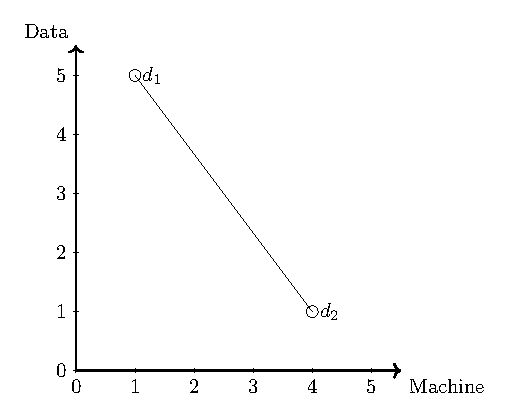
\includegraphics[width=0.7\linewidth,height=\textheight,keepaspectratio,alt={Documents in a two-dimensional space}]{chapters/../assets/figures/chapter11/ch-text-2d.pdf}

}

\caption{\label{fig-text-2d}Documents in a two-dimensional space}

\end{figure}%

With this dimensional representation, pair-wise similarity or difference
can be measured by the geometric distance between two document data
points. A classic metric of such is the \emph{Euclidean Distance}, which
measures the length of the straight line connecting the two data points
in question, as shown in Figure~\ref{fig-text-2d}. In an
\(m\)-dimensional space, the general \emph{Euclidean Distance} function
is:

\[\begin{aligned}
  ED(u,v) & = & \sqrt{\sum_{i=1}^{m} (u_i - v_i)^2}
\end{aligned}\]

where \(u_i\) and \(v_i\) are the \(i^{th}\) dimensional value of data
points \(u\) and \(v\) respectively. Given documents \(d_1\) and \(d_2\)
in Figure~\ref{fig-text-2d}, their euclidean distance is:

\[\begin{aligned}
  ED(d_1,d_2)
  & = & \sqrt{(5-1)^2 + (1-4)^2}   \\
  & = & 5
\end{aligned}\]

While \emph{Euclidean Distance} is widely used in text mining, its
performance may suffer in applications where there is a wide
distribution of document sizes. A thought experiment will help
illustrate the problem.

Imagine we have two documents \(d_1 = (4,5)\) and \(d_2=(5,4)\) (with TF
weights) that are highly similar and have a very small Euclidean
distance between them, as show in Figure~\ref{fig-text-thought}:

\begin{figure}

\centering{

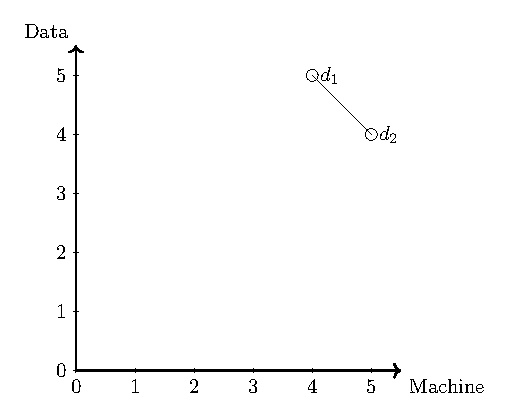
\includegraphics[width=0.7\linewidth,height=\textheight,keepaspectratio,alt={Thought experiment with two documents}]{chapters/../assets/figures/chapter11/ch-text-thought.pdf}

}

\caption{\label{fig-text-thought}Thought experiment with two documents}

\end{figure}%

For now, one may think the line distance in
Figure~\ref{fig-text-thought} is a reasonable estimate of their
difference. But imagine make a double-copy of \(d_2\) and treat the new
copy as \(d_3\), resulting in Figure~\ref{fig-text-thought}:

\begin{figure}

\centering{

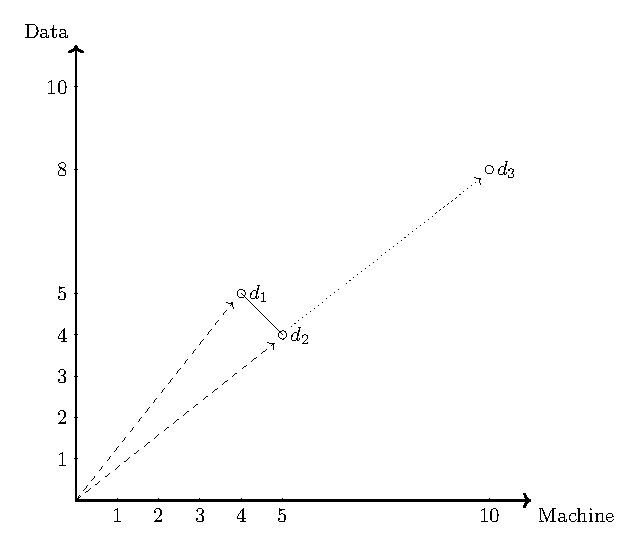
\includegraphics[width=0.7\linewidth,height=\textheight,keepaspectratio,alt={Thought experiment a third document, where d\_3 doubles the content of d\_2}]{chapters/../assets/figures/chapter11/ch-text-thought2.pdf}

}

\caption{\label{fig-text-thought2}Thought experiment a third document,
where \(d_3\) doubles the content of \(d_2\)}

\end{figure}%

Because \(d_3\) is copy of \(d_2\) -- the only difference is that it
doubles everything in \(d_2\) -- its semantics should remain the same as
\(d_2\). A fair distance measure should give a relatively small value,
indicating \(d_3\) is \emph{close} to \(d_1\) and especially \(d_2\).
However, as shown in Figure~\ref{fig-text-thought}, \(d_3\) is much
farther away from \(d_1\) and consequently the euclidean distance is
much greater.

In short, Euclidean Distance treats documents differently simply because
they are of different sizes (magnitude). In this light, we should
somehow disregard the sizes when measuring their similarities.

Another perspective on similarity vs.~distance in the dimensional space
is by measuring the \emph{direction} of a vector. In physics, the notion
of vector has been used extensively for quantities such as velocity,
which has both a \emph{magnitude} (speed) and direction. Likewise, as
shown as dashed lines in Figure~\ref{fig-text-thought2}, documents such
as \(d_1\) and \(d_2\) can be treated as vectors from the origin, with a
magnitude (line length) and direction (arrow). The difference between
the two documents can be measured by their angle distance.

Also in Figure~\ref{fig-text-thought2}, \(d_3\) as copy of \(d_2\) is
pointing in the exact same direction of \(d_2\) and their angle distance
is \(0\). Consequently, the angle distance between \(d_1\) and \(d_3\)
is the same as that of \(d_1\) and \(d_2\).

All this makes sense with angle distance as \(d_2\) and \(d_3\)
essentially have the same content and should be treated equivalent. In
this \emph{vector space} representation, a vector's direction is
dependent on the \emph{distribution of term weights} in the
corresponding text document. While the magnitude is about the absolute
values of term weights, the direction is a rather relative measure --
that means, in the case of Figure~\ref{fig-text-thought2}, to what
degree a document vector is more or less about \emph{machine} (to the
east) vs.~\emph{data} (to the north).

To measure an \emph{angle distance}, one can calculate the degree of the
angle between two vectors. Nonetheless, a classic approach is to measure
the \emph{cosine} of the angle as their \emph{similarity}.

\begin{figure}

\centering{

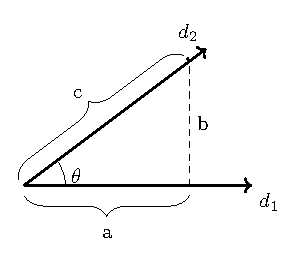
\includegraphics[width=0.7\linewidth,height=\textheight,keepaspectratio,alt={Cosine of an angle}]{chapters/../assets/figures/chapter11/ch-text-cosine.pdf}

}

\caption{\label{fig-text-cosine}Cosine of an angle}

\end{figure}%

As shown in Figure~\ref{fig-text-cosine}, with the help line
perpendicular to vector \(d_1\), the cosine of \(d_1\) and \(d_2\) is:

\[\begin{aligned}
  Cosine(d_1, d_2)
  & = & \frac{a}{c}
\end{aligned}\]

With the vector representations of any two documents \(u\) and \(v\),
the same cosine can be computed by:

\[\begin{aligned}
Cosine(d_u, d_v)
& = & \frac{\sum_{i=1}^{m} u_i v_i}{\sqrt{\sum_{i=1}^{m} u_i^2} \sqrt{\sum_{i=1}^{m} v_i^2}}
\end{aligned}\]

where \(u_i\) is the weight of the \(i^{th}\) term in document \(u\) and
\(v_i\) is the same term's weight in document \(v\). For the three
documents in the thought experiments, \(d_1=(4,5)\), \(d_2=(5,4)\), and
\(d_3=(10,8)\), we can compute their pairwise similarities:

\[\begin{aligned}
Cosine(d_1, d_2)
& = & \frac{4*5 + 5*4}{\sqrt{4^2+5^2}\sqrt{5^2+4^2}}  \\
& \approx & 0.98  \\
Cosine(d_1, d_3)
& = & \frac{4*10 + 5*8}{\sqrt{4^2+5^2}\sqrt{10^2+8^2}}  \\
& \approx & 0.98  \\
Cosine(d_1, d_2)
& = & \frac{4*8 + 5*10}{\sqrt{4^2+5^2}\sqrt{10^2+8^2}}  \\
& = & 1  \\
\end{aligned}\]

In this case, \(d_1\) and \(d_2\) are identical with cosine \(1\)
whereas \(d_2\) and \(d_3\) have the same similarity compared to
\(d_1\).

Cosine is inversely related to the angle \(\theta\) (distance) and is a
similarity measure. When two vectors are close in their direction, with
a small angle shown in Figure~\ref{fig-text-cosine2}, \(a\) is almost
the same as \(c\) and cosine similarity is nearly \(1\). The two vectors
are highly similar in their directions, with \(1\) indicating the same
direction and perfect match.

\begin{figure}

\centering{

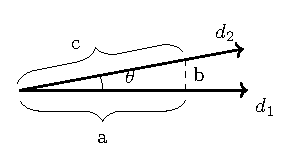
\includegraphics[width=0.7\linewidth,height=\textheight,keepaspectratio,alt={Cosine of a small angle, i.e. vectors of close directions}]{chapters/../assets/figures/chapter11/ch-text-cosine2.pdf}

}

\caption{\label{fig-text-cosine2}Cosine of a small angle, i.e.~vectors
of close directions}

\end{figure}%

On the other hand, when two vectors point to directions nearly
perpendicular to one another, with a large angle shown in
Figure~\ref{fig-text-cosine3}, \(a\) becomes extremely small and cosine
similarity is close to \(0\). For vectors based on text documents, their
vector values are normally positive (in the first quadrant in the
two-dimensional space). Therefore, the smallest cosine similarity value
one can obtain is \(0\) when two vectors are exactly perpendicular
(orthogonal directions).

\begin{figure}

\centering{

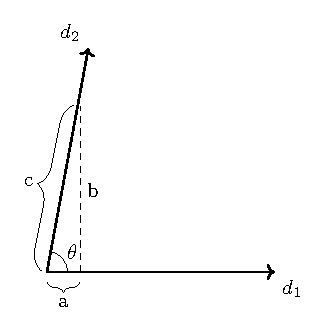
\includegraphics[width=0.7\linewidth,height=\textheight,keepaspectratio,alt={Cosine of a large angle, i.e. vectors with nearly perpendicular directions}]{chapters/../assets/figures/chapter11/ch-text-cosine3.pdf}

}

\caption{\label{fig-text-cosine3}Cosine of a large angle, i.e.~vectors
with nearly perpendicular directions}

\end{figure}%

In short, cosine is a similarity measure in the vector space model,
which ranges from \(0\) and \(1\). A greater cosine value indicates a
higher similarity of two vectors.

\section{Probabilities and
Implications}\label{probabilities-and-implications}

\subsection{Zipf's Law}\label{zipfs-law}

The notion of \emph{least action} or \emph{least effort} has long been
observed in the natural world as well as human behavior. In spoken
language, we tend to minimize our efforts by reusing old words and
expressions, as if they are old tools meant for many applications. The
results of this: words tend toward "a minimum in number and size" and
"the older the tool (word) the more different jobs it can perform."(Zipf
1949)

Under the \emph{Principle of Least Effort}, there appears to be a great
divide between a small number of words so frequently used and those
rarely mentioned. In particular, if we sort words by their frequencies,
a term \(t\)'s frequency \(f_t\) is proportional to the inverse of its
rank \(k_t\):

\[\begin{aligned}
  f_t & \propto & \frac{1}{k_t}
\end{aligned}\]

where word \(t\) is ranked the \(k^{th}\) most frequent. If we consider
probabilities rather than raw frequencies, the above can be written as:

\[\begin{aligned}
  p(t) & = & \frac{c}{k_t}
\end{aligned}\]

where \(c\) is a constant. In the English language, empirical data have
shown \(p(t) \approx 0.1 / k_t\) within the top \(1,000\) rank. This
relation can be visualized in Figure~\ref{fig-text-zipf} (a).

\begin{figure}

\centering{

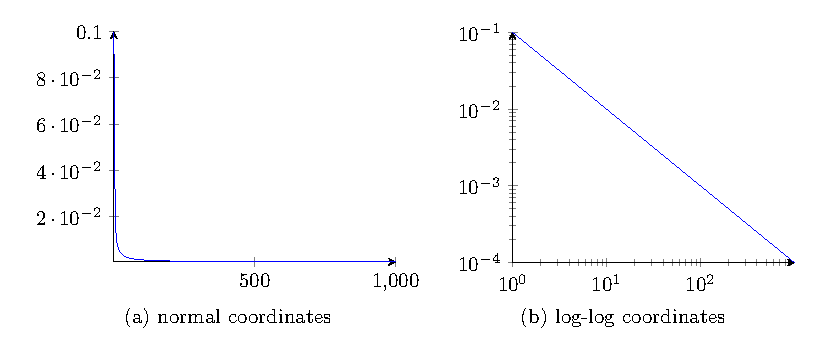
\includegraphics[width=0.7\linewidth,height=\textheight,keepaspectratio,alt={Zipf law function, roughly for the top 1,000 in English}]{chapters/../assets/figures/chapter11/fig-text-zipf.pdf}

}

\caption{\label{fig-text-zipf}Zipf law function, roughly for the top
\(1,000\) in English}

\end{figure}%

With a long tail, Figure~\ref{fig-text-zipf} (a) on normal coordinates
is difficult to examine and it is often useful to apply the logarithmic
transformation. By taking the log of both \(x\) (rank) and \(y\)
(frequency) values, this can be transformed into
Figure~\ref{fig-text-zipf} (b). As shown, Zipf law is a linear function
on log-log coordinates and is a special case of \emph{power-law}
distributions, which, as we discussed in Chapter~, are results of the
\emph{Matthew effect} (the rich get richer). In fact, there is an
intrinsic connection between the \emph{Principle of Least Effort} and
the \emph{Matthew effect} -- as we tend to a minimum set of vocabulary,
what we have frequently used (old "rich" words) will be used even more
frequently (richer).

\subsection{Feature Selection}\label{feature-selection}

We have observed that any text processing may involve a very large
number of features (terms) and it is a common practice to perform
\emph{feature selection} in such processes as clustering,
classification, and retrieval (search).

In light of Zipf's law, there are a large number of words that are
rarely used, only in a few documents. While these terms might be
informative when they occur, their rare occurrences make them less
useful in such tasks as clustering and classification where documents
are grouped by terms they have in common. Given that there are many low
frequent words -- the long tail of the Zipf function -- removing them
will reduce the dictionary size (feature space) significantly.

In terms of document frequency (DF), on the other hand, we know highly
frequent words such as stop words are not informative and can be safely
removed in certain applications. In practice, simple feature selection
techniques such as DF (document frequency) thresholding has performed
very effectively with little computational cost.(Yang and Pedersen 1997)
It has been shown that having the right number of features is key to the
success of text clustering and classification -- using all features not
only slows down the processing but also contributes more noise than
information for related tasks.(Ke 2015)

\section{Text Classification}\label{text-classification}

With a distance or similarity measure in the vector representation, it
is now possible to compare documents to one another and associate them
with data groups or labels. For example, one may use an instance-based
lazy learning method such as kNN (see
Chapter~\hyperref[ch-choices]{{[}ch-choices{]}}) with cosine similarity
to perform classification and prediction based on the nearest data
vectors.

Another successful approach is to model the probability that a document
belongs to each class (label) and assign the document to the class that
maximizes the probability. That is, given a document representation
\(d\), we need to estimate the probability of each class \(p(c_i|d)\),
where \(c_i\) is one of the given classes to be predicted.

Say we are working on email \emph{spam} filtering based on subject
titles. This is a binary classification problem, for which we have two
classes (labels) -- an email is either a \emph{ham} (normal) or a
\emph{spam} (junk). Suppose we have a small collection of email subjects
which we have labeled \emph{ham} or \emph{spam} to train our model
(learning):

{\def\LTcaptype{none} % do not increment counter
\begin{longtable}[]{@{}clc@{}}
\toprule\noalign{}
DOC & Email Subject & Class \\
\midrule\noalign{}
\endhead
\bottomrule\noalign{}
\endlastfoot
1 & You have been selected! & spam \\
2 & Have a prize for you! & spam \\
3 & You won! & spam \\
4 & Project meeting schedule & ham \\
5 & Nice to meet you! & ham \\
6 & Project update & ham \\
7 & Update on research & ham \\
\end{longtable}
}

\protect\phantomsection\label{tab-text-emails}{}

\subsection{Naive Bayes with Binary Term Occurrences
(Bernoulli)}\label{naive-bayes-with-binary-term-occurrences-bernoulli}

Given the short subject titles, let us first look at how we can model
probabilities in text if we only consider binary occurrences of terms.
Assume we remove some of stop-words (e.g.~have, been) and normalize some
others (e.g.~meeting \(\to\) meet, won \(\to\) win), we can represent
the email using the following dictionary:

{\def\LTcaptype{none} % do not increment counter
\begin{longtable}[]{@{}lccccccccccl@{}}
\toprule\noalign{}
& 1 & 2 & 3 & 4 & 5 & 6 & 7 & 8 & 9 & 10 & \\
\midrule\noalign{}
\endhead
\bottomrule\noalign{}
\endlastfoot
DOC & meet & nice & prize & project & research & schedule & select &
update & win & you & Class \\
1 & & & & & & & 1 & & & 1 & spam \\
2 & & & 1 & & & & & & & 1 & spam \\
3 & & & & & & & & & 1 & 1 & spam \\
4 & 1 & & & 1 & & 1 & & & & & ham \\
5 & 1 & 1 & & & & & & & & 1 & ham \\
6 & & & & 1 & & & & 1 & & & ham \\
7 & & & & & 1 & & & 1 & & & ham \\
\end{longtable}
}

\protect\phantomsection\label{tab-text-emails_bin}{}

Within a class \(c\), there is a probability that a term \(t\) will
occur in a (random) document \(p(t|c)\). To estimate the probability,
one can simply count the ratio between the number of emails \(t\)
appears and the total number of emails in class \(c\).

However, as we discussed in Chapter~, this approach may lead to skewed
estimates and potential zero probability values due to data variance in
the sample. Now that we have a very small data set here, we will use the
Laplace estimator with an added constant \(\mu\) to any count, that is:

\[\begin{aligned}
  p(t|c) & = & \frac{n(t|c)+\mu}{N(c)+2\mu}
\end{aligned}\]

where \(n(t|c)\) is the number of documents in class \(c\) that contain
term \(t\) (document frequency) and \(N(c)\) is the total number of
documents belonging to \(c\). \(\mu\) is a constant added to avoid zero
probability estimates and \(2\mu\) in the denominator is to account for
\(\mu\) being added to the binary cases (for when \(t\) occurs and when
it does not).

For example, with \(\mu=0.05\), some of the term probabilities in the
spam class can be computed by:

\[\begin{aligned}
  p(meet|spam)  & = & (0+0.05)/(3+0.1) \\
                & = & 0.016 \\
  p(prize|spam) & = & (1+0.05)/(3+0.1) \\
                & = & 0.339 \\
  p(you|spam)   & = & (3+0.05)/(3+0.1) \\
                & = & 0.984
\end{aligned}\]

The same probabilities in the ham class are:

\[\begin{aligned}
  p(meet|ham)  & = & (2+0.05)/(4+0.1)  \\
                & = & 0.5 \\
  p(prize|ham) & = & (0+0.05)/(4+0.1) \\
                & = & 0.012 \\
  p(you|ham)   & = & (1+0.05)/(4+0.1) \\
                & = & 0.256
\end{aligned}\]

In the binary representation, \(w_t = 1\) when term \(t\) occurs in the
document and \(w_t = 0\) if it does not. Given \(p(t|c)\) probability
term \(t\) occurs in a (random) document in class \(c\), \(1 - p(t|c)\)
is the probability that it does not occur. That is, the probability of
observing a binary term weight \(w_t\) can be written as the
\emph{Bernoulli} probability mass function:

\[\begin{aligned}
  p(w_t|c)
  & = & p(t|c)^{w_t} (1-p(t|c))^{1-w_t} \\
  & = &
  \begin{cases}
    p(t|c), & \text{if}\ w_t = 1 \\
    1-p(t|c), & \text{otherwise}\ w_t = 0
  \end{cases}
\end{aligned}\]

For term \emph{prize} in the spam class, the above can be written as:

\[\begin{aligned}
  p(w_{prize}|spam)
  & = & p(prize|spam)^{w_{prize}} (1-p(prize|spam))^{1-w_{prize}} \\
  & = &
  \begin{cases}
    0.339, & \text{if prize occurs}\ w_{prize} = 1 \\
    0.661, & \text{otherwise}\ w_{prize} = 0
  \end{cases}
\end{aligned}\]

Similarly, probability of a term weight for \emph{you} in the ham class:

\[\begin{aligned}
  p(w_{you}|ham)
  & = & p(you|ham)^{w_{prize}} (1-p(you|spam))^{1-w_{you}} \\
  & = &
  \begin{cases}
    0.256, & \text{if it occurs}\ w_{you} = 1 \\
    0.744, & \text{otherwise}\ w_{you} = 0
  \end{cases}
\end{aligned}\]

Following this, we can estimate the probability of \emph{any} term
weight \(w_t\) in the classes ham vs.~spam. Now suppose we receive a new
email and try to determine whether it is a \emph{ham} or a \emph{spam}:

\protect\phantomsection\label{tab-text-emails_new}
\begin{longtable}[]{@{}clc@{}}
\caption{A new email to be classified}\tabularnewline
\toprule\noalign{}
DOC & Email Subject & Class \\
\midrule\noalign{}
\endfirsthead
\toprule\noalign{}
DOC & Email Subject & Class \\
\midrule\noalign{}
\endhead
\bottomrule\noalign{}
\endlastfoot
\(d\) & Your prize! & ? \\
\end{longtable}

\protect\phantomsection\label{tab-text-emails_new}{}

which can be represented as:

{\def\LTcaptype{none} % do not increment counter
\begin{longtable}[]{@{}lccccccccccl@{}}
\toprule\noalign{}
& 1 & 2 & 3 & 4 & 5 & 6 & 7 & 8 & 9 & 10 & \\
\midrule\noalign{}
\endhead
\bottomrule\noalign{}
\endlastfoot
DOC & meet & nice & prize & project & research & schedule & select &
update & win & you & Class \\
\(d\) & & & 1 & & & & & & & 1 & ? \\
\end{longtable}
}

\protect\phantomsection\label{tab-text-new_bin}{}

The question here is how we can estimate the probability of the email
\(d\) being \emph{ham} or \emph{spam}, \(p(ham|d)\) vs.~\(p(spam|d)\).
Using the Bayes theorem, they can be computed by:

\[\begin{aligned}
  p(ham|d) & = & \frac{p(ham)p(d|ham)}{p(d)} \\
  p(spam|d) & = & \frac{p(spam)p(d|spam)}{p(d)} 
\end{aligned}\]

Both equations above have \(p(d)\) as the denominator, which does not
affect the ratio of the two values (classification outcome) and can be
ignored in the calculation.

\(p(ham)\) and \(p(spam)\) can be estimated by counting the number of
hams vs.~spams. With a Laplace estimator, they are:

\[\begin{aligned}
  p(ham)  & = & (4+0.05)/(7+0.1) \\
                & = & 0.57 \\
  p(spam)   & = & (3+0.05)/(7+0.1) \\
                & = & 0.43 \\
\end{aligned}\]

For \(p(d|spam)\), email \(d\) can be viewed as a collection of its term
weights \(w_t\). Given the \(10\) terms in the dictionary, \(p(d|spam)\)
is their joint probabilities \(p(w_t|spam)\) in the \emph{spam} class.
Assume the term probabilities are independent (naive assumption), the
conditional probability can be computed by:

\[\begin{aligned}
  p(d|spam)
  & = & \prod_{t} p(w_{dt}|spam) \\
  & = & p(w_{meet}=0|spam) p(w_{nice}=0|spam) p(w_{prize}=1|spam) ... p(w_{you}=1|spam) \\
  & = & 0.984 \times 0.984 \times 0.339 ... \times 0.984 \\
  & = & 0.132
\end{aligned}\]

Likewise, we can compute the probability conditioned on the \emph{ham}
class:

\[\begin{aligned}
  p(d|ham)
  & = & \prod_{t} p(w_{dt}|ham) \\
  & = & p(w_{meet}=0|ham) p(w_{nice}=0|ham) p(w_{prize}=1|ham) .. p(w_{you}=1|ham) \\
  & = & 0.5 \times 0.744 \times 0.012 ... \times 0.256 \\
  & = & 0.013
\end{aligned}\]

Plug the numbers back in
Equations~\hyperref[eq-text-nb_ham]{{[}eq-text-nb\_ham{]}} and
\hyperref[eq-text-nb_spam]{{[}eq-text-nb\_spam{]}}, we have:

\[\begin{aligned}
  p(spam|d)
  & = & \frac{p(spam)p(d|spam)}{p(d)}  \\
  & = & \frac{0.43 \times 0.293}{p(d)} \\
  & = & \frac{0.132}{p(d)} \\
  p(ham|d)
  & = & \frac{p(ham)p(d|ham)}{p(d)} \\
  & = & \frac{0.57 \times 0.013}{p(d)} \\
  & = & \frac{0.007}{p(d)} \\
\end{aligned}\]

Clearly \(p(ham|d) < p(spam|d)\) and the new email \(d\) will be
predicted as a spam.

Two important notes here. First, although the example only has two
classes, the Naive Bayes classifier can be applied to more than two
classes. Given a document \(d\) and a set of classes
\(C = [c_1, c_2, .., c_k]\), where \(k \ge 2\), the general Naive Bayes
model with Bernoulli distribution is to identify a class \(\hat{c}\)
such that the posterior probability \(p(c|d)\) is maximized:

\[\begin{aligned}
  \hat{c}
  & = & \mathop{\mathrm{arg\,max}}_{c \in C} p(c|d) \\
  & = & \mathop{\mathrm{arg\,max}}_{c \in C} \frac{p(c)p(d|c)}{p(d)} \\
  & = & \mathop{\mathrm{arg\,max}}_{c \in C} \frac{p(c)\prod_{t} p(w_{dt}|c)}{p(d)}
\end{aligned}\]

where \(w_{dt}\) is the binary weight of term \(t\) in document \(d\)
(to be classified). \(p(d)\) is the common denominator for all classes
and can be ignored in the calculation.

Second, the product of joint probabilities (with \(\prod_t\) in the
above equation) in the model can become a very small value, especially
when there are a great number of terms in the dictionary. To avoid this
computational difficulty, it is a better practice to convert this into a
log-likelihood (by taking the logarithm of the probabilities):

\[\begin{aligned}
  \hat{c}_{log}
  & = & \mathop{\mathrm{arg\,max}}_{c \in C} \log \frac{p(c)\prod_{t} p(w_{dt}|c)}{p(d)} \\
  & = & \mathop{\mathrm{arg\,max}}_{c \in C} \log p(c) + \sum_{t} \log p(w_{dt}|c) - \log p(d)
\end{aligned}\]

In this way, we perform the addition of log-likelihood and can maintain
a better precision with float points. Again \(\log p(d)\) is a constant
across the classes and can be omitted in the computing.

\subsection{Naive Bayes with Term Frequencies
(Multinomial)}\label{naive-bayes-with-term-frequencies-multinomial}

Now let us look beyond binary term occurrences for text classification.
As we discussed earlier in the chapter, term frequency (TF) is a useful
statistic, which we should also take advantage of in this task.

Suppose we extend the email representation from subject title to include
email body (content) as well. Assume the dictionary (vocabulary) remains
the same as in
Table~\hyperref[tab-text-emails_bin]{{[}tab-text-emails\_bin{]}} but
obviously terms may occur multiple times in the email text. The
following is a hypothetical TF representation of the same emails:

{\def\LTcaptype{none} % do not increment counter
\begin{longtable}[]{@{}lccccccccccl@{}}
\toprule\noalign{}
& 1 & 2 & 3 & 4 & 5 & 6 & 7 & 8 & 9 & 10 & \\
\midrule\noalign{}
\endhead
\bottomrule\noalign{}
\endlastfoot
DOC & meet & nice & prize & project & research & schedule & select &
update & win & you & Class \\
1 & & & & & & & 1 & & & 3 & spam \\
2 & & & 3 & & & & & & & 2 & spam \\
3 & & & & & & & & & 2 & 2 & spam \\
4 & 2 & & & 1 & & 3 & & & & & ham \\
5 & 1 & 1 & & & & & & & & 2 & ham \\
6 & & & & 2 & & & & 1 & & & ham \\
7 & & & & & 3 & & & 1 & & & ham \\
\end{longtable}
}

\protect\phantomsection\label{tab-text-emails_tf}{}

The probability of term \(t\) in class \(c\), \(p(t|c)\) can be computed
by its overall term frequency (in all documents) over the total term
frequency of documents in that class. Given term frequencies in
Table~\hyperref[tab-text-emails_tf]{{[}tab-text-emails\_tf{]}}, the
following terms' probabilities in the spam class can be estimated
by\footnote{Again, we add a Laplace constant of \(1\), which is \(1\)
  added to the numerator and \(2\) added to the denominator.}:

\[\begin{aligned}
  p(nice|spam)  & = & (0+1)/[(1+3+3+2+2+2)+2] \\
                & = & 1/15 \\
  p(prize|spam) & = & (3+1)/15 \\
                & = & 4/15 \\
  p(you|spam)   & = & (3+2+2+1)/15 \\
                & = & 8/15
\end{aligned}\]

Likewise, these terms' probabilities in the ham class can be estimated
by:

\[\begin{aligned}
  p(nice|ham)  & = & (1+1)/[(2+1+3+1+1+2+2+1+3+1)+2] \\
                & = & 2/19 \\
  p(prize|ham) & = & (0+1)/19 \\
                & = & 1/19 \\
  p(you|ham)   & = & (2+1)/19 \\
                & = & 3/19
\end{aligned}\]

Now given the following new document to be classified:

{\def\LTcaptype{none} % do not increment counter
\begin{longtable}[]{@{}lccccccccccl@{}}
\toprule\noalign{}
& 1 & 2 & 3 & 4 & 5 & 6 & 7 & 8 & 9 & 10 & \\
\midrule\noalign{}
\endhead
\bottomrule\noalign{}
\endlastfoot
DOC & meet & nice & prize & project & research & schedule & select &
update & win & you & Class \\
\(d\) & & 1 & 3 & & & & & & & 2 & ? \\
\end{longtable}
}

\protect\phantomsection\label{tab-text-new_tf}{}

Document \(d\) can be regarded as a sequence of terms that are drawn
from their probability distributions. And the probability of generating
the document \(p(d)\) is proportional to the joint probability of
drawing the individual terms, following the Multinomial
distribution\footnote{With the bag-of-words approach, the Multinomial
  probability mass function has to include as a factor
  \(\frac{n_d!}{\prod_t TF_{dt}!}\) because of the permutations the
  terms can appear in. This Multinomial coefficient, however, is a
  constant given a fixed document \(d\), is the same for all classes and
  can be omitted.}:

\[\begin{aligned}
  p(d)
  & \propto & \prod_{k=1}^{n_d} p(t_k) \\
  & = & \prod_{t \in T} p(t)^{TF_{dt}}
\end{aligned}\]

where \(n_d\) is the length of document \(d\) (the total number of terms
including duplicates) and \(t_k\) is term \(t\) at position of \(k\) in
the document. In the bag-of-words approach, positional information is
irrelevant so \(p(t_k) = p(t)\) for any position \(k\). \(T\) is the
dictionary of unique terms, and \(TF_{dt}\) is term frequency of term
\(t\) in document \(d\).

If document \(d\) belongs to be particular class \(c\), the posterior
probability can be computed in the same manner:

\[\begin{aligned}
  p(d|c)
  & = & \prod_{t \in T} p(t|c)^{TF_{dt}}
\end{aligned}\]

For document \(d\) in
Table~\hyperref[tab-text-new_tf]{{[}tab-text-new\_tf{]}}, IF it belongs
to the spam class, then the log-likelihood of having document \(d\)
is\footnote{Note that in the calculation we omit terms that do not occur
  in document because a \(0\) TF value will lead to \(0\) in the
  log-likelihood and does not affect the result.}:

\[\begin{aligned}
  \log p(d|spam)
  & = & \log \prod_{t \in T} p(t|spam)^{TF_{dt}} \\
  & = & \sum_{t \in T} TF_{dt}\log p(t|spam) \\
  & = & 1 \log p(nice|spam) + 3 \log p(prize|spam) + 2 \log p(you|spam) \\
  & = & \log \frac{1}{15} + 3 \log \frac{4}{15} + 2 \log \frac{8}{15} \\
  & = & - 3.444
\end{aligned}\]

Likewise, we can compute the log-likelihood of \(d\) IF it belongs to
the \emph{ham} class instead:

\[\begin{aligned}
  \log p(d|ham)
  & = & \sum_{t \in T} TF_{dt}\log p(t|ham) \\
  & = & 1 \log p(nice|ham) + 3 \log p(prize|ham) + 2 \log p(you|ham) \\
  & = & \log \frac{2}{19} + 3 \log \frac{1}{19} + 2 \log \frac{3}{19} \\
  & = & - 6.417
\end{aligned}\]

Finally, we can estimate the posterior probability of document \(d\)
belonging to either spam or ham by using the Bayes theorem. Again, the
log-likelihood is used:

\[\begin{aligned}
  \log p(spam|d)
  & = & \log \frac{p(spam)p(d|spam)}{p(d)} \\
  & = & \log p(spam) + \log p(d|spam) - \log p(d) \\
  & = & \log 0.43 - 3.444 - \log p(d) \\
  & = & - 3.811 - \log p(d) \\
  \log p(ham|d)
  & = & \log \frac{p(ham)p(d|ham)}{p(d)} \\
  & = & \log p(ham) + \log p(d|ham) - \log p(d) \\
  & = & \log 0.57 - 6.417 - \log p(d) \\
  & = & - 6.66 - \log p(d)
\end{aligned}\]

In this case, \(\log p(spam|d)> \log p(ham|d)\) so
\(p(spam|d)> p(ham|d)\) and document \(d\) should be labeled a spam.

Back to the general model of Naive Bayes with a Multinomial
distribution, the idea is to consider term frequencies in the model and
identify the class that maximizes the log-likelihood of the document's
membership to that class. That is\footnote{Here we omit \(\log p(d)\) as
  it is constant for all classes.}:

\[\begin{aligned}
  \hat{c}
  & = & \mathop{\mathrm{arg\,max}}_{c \in C} \log p(c)\prod_{t} p(t|c)^{TF_{dt}} \\
  & = & \mathop{\mathrm{arg\,max}}_{c \in C} \log p(c) + \sum_{t \in T} TF_{dt} \log p(t|c)
\end{aligned}\]

where \(c\) is each class in the set of classes \(C\), \(t\) is each
term in dictionary \(T\), \(p(t|c)\) is the probability of term \(t\) in
class \(c\), and \(TF_{dt}\) is the term frequency of \(t\) in document
\(d\), the document to be classified.

\section*{Summary}\label{text-summary}
\addcontentsline{toc}{section}{Summary}

\markright{Summary}

The basic method for text processing is the \emph{bag of words}
approach, in which we disregard the order of \emph{tokens}. In practice,
for the English language, tokens are often single words which can be
obtained using word boundaries such as space and punctuation.
Nonetheless, a token can be a phrase or any number of characters in a
sequence (character n-gram). For example, you may treat every four
consecutive characters (4-gram) in a document as a token and use all
unique 4-gram tokens as your vocabulary.

Some form of token normalization can be helpful. However, the extent of
its use depends on the language, data domain, and use cases, e.g.~how
users express their queries vs.~words used in written documents of the
data collection.

Once tokens or terms are obtained and normalized, we can then assign
certain weights to them for the representation of text documents. We
have discussed term weighting schemes including the binary, term
frequency (TF), and TF*IDF (Inverse Document Frequency). TF*IDF is a
classic treatment where a term's weight increases with the increase of
term frequency in the current document and its rarity in other
documents. IDF, or a term's rarity, indicates the degree of
\emph{specificity} and \emph{informativeness} of the term.

Text documents can be treated as vectors based on the term weights. When
comparing two vectors in the vector space model, we noticed that vector
direction is more important than vector magnitude (length). Whereas the
magnitude is a function of the absolute values of term weights, the
vector direction is due to the distribution of these (relative) weights.
Because of this nature, we often use an angle-based distance function
such as cosine similarity to compare two vectors.

The probabilistic view provides an important approach to text
processing. The Zipf's is an empirical generalization of the
probabilistic occurrences of spoken or written words. The Bayes theorem
lays the foundation for probabilistic modeling of problems such as text
classification and retrieval.

\chapter{Search and Retrieval}\label{ch-search}

Ask, and it shall be given you; seek, and you shall find; knock, and it
shall be opened to you.

\emph{The Gospel of Matthew}

We are in constant pursuit of information, knowledge, and truth. We have
questions and we ask. Today, we ask questions and seek information with
the help of technologies. We search for information and web pages by
Googling. We pose questions to digital assistants such as Amazon's
Alexa. Regardless of differences in the specifics, the essence of these
interactions is to find the right (relevant) piece of information that
can satisfy us (the user) -- be it a web page, a short answer, a
prediction or some kind of recommendation.

This is about search and the general area of research is commonly
referred to as \emph{Information Retrieval}. In 1951 -- when searches
for information were primarily conducted in the libraries with the
assistance of reference librarians without a computer -- Calvin Mooers
coined the term \emph{Information Retrieval} as "the investigation of
information description and specification for search and techniques for
search operations."(Mooers 1951) A library catalog with index cards was
the state of the art to help people seek and find quickly.

With the support of computers, we can perform the same type of search
tasks even more efficiently, yet with ease on the user's side and
sophistication on the system's side. Now that computers are essential to
the various search systems we have in place, the notion of
\emph{Information Retrieval} (IR) may be redefined, in a narrower sense,
as:(Manning et al. 2008)

finding material (usually documents) of an unstructured nature (usually
text) that satisfies an information need from within large collections
(usually stored on computers)

With this narrower definition, a basic task of IR is, given a user
query, to find \emph{relevant} documents from a collection of text
materials. Traditionally, the data collection such as a library of books
is assumed to be static, and certain pre-computation and indexing can be
conducted before querying processing. In reality, this assumption does
rarely hold as data can grow to include new materials which in turn
should be incorporated into the index.

Web search engines are \emph{Information Retrieval} (IR) systems and the
Web is a huge collection of data that constantly grow and change. The
magnitude, dynamics, and decentralization of data on the Web pose great
challenges, which have led to waves of innovation on Web IR\footnote{First
  came Lycos and Yahoo, which borrowed traditional text indexing and
  reference catalog/directory techniques from libraries. AltaVista
  enhanced the technologies with a larger index and a responsive
  interface. Google and Baidu came after them and revolutionized search
  ranking by using \emph{citation analysis}, another method that had
  been studied extensively in library science. Now very few people know
  AltaVista, not to mention Lycos. Looking forward, what will come in
  the next ten or twenty years? Will Google remain relevant then.}. We
will discuss some of these challenges and related ideas later in the
chapter.

\section{Basic Paradigm}\label{basic-paradigm}

In information retrieval, the basic problem is to search and find
matched documents against a query representation based on a user's
information need. Documents need to be stored in proper representation
so that related matches can be computed (numerically). An index is also
necessary to conduct the matching process timely.

As shown in Figure~\ref{fig-ir}, the user with an information need
issues a query to the retrieval system, which in turn match it against
the document representation in the store to identify relevant documents
in the search result. The result can also be ranked (sorted) in terms of
predicted relevance of each document.

\begin{figure}

\centering{

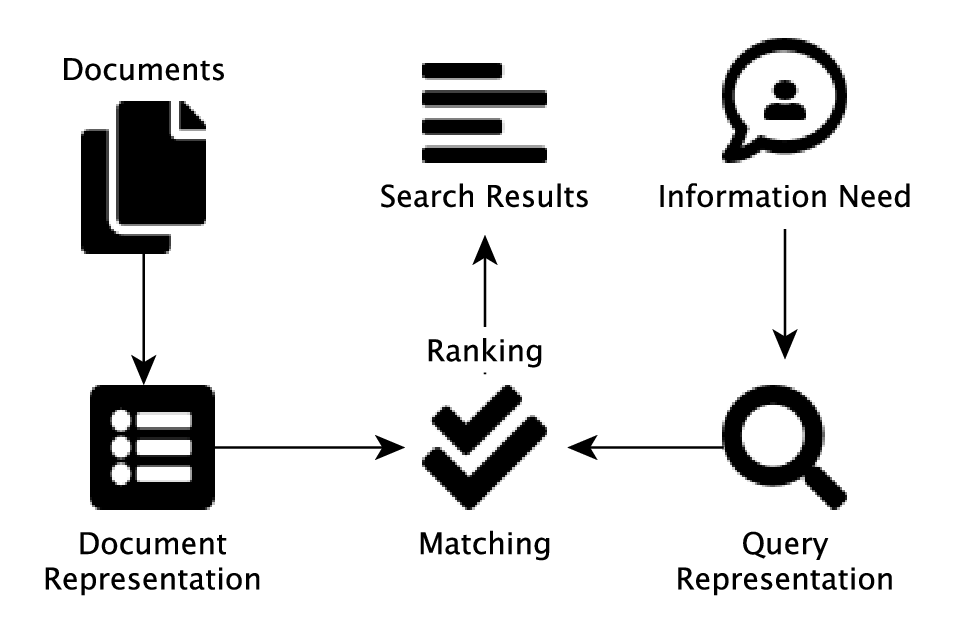
\includegraphics[width=3.5in,height=\textheight,keepaspectratio,alt={Basic paradigm of an Information Retrieval system}]{chapters/../assets/figures/ir2.png}

}

\caption{\label{fig-ir}Basic paradigm of an \emph{Information Retrieval}
system}

\end{figure}%

The notion of \emph{relevance} is key in information retrieval research.
Yet it remains one of the least understood concepts in the field.
Whether a piece of information is relevant depends on many factors such
as the user's objectives and the context of the current task. Sometimes,
these may be difficult for the user to articulate; and even if she does,
the query expression thus constructed may hardly be precise.

Retrieval systems have to attack the issue of uncertainty often
associated with understanding the user's need and what is truly relevant
in context. We can factor this in when building a retrieval model. With
probabilistic models, for example, the degree of uncertainty can be
quantified for proper probabilistic ranking in light of probability and
information theories.

However, uncertainty is often due to lack of information (data) and
requires further data collection. Techniques that support relevance
feedback and interactive, exploratory searching may help engage the user
in order to understand more precisely what she is looking for.

\section{Indexing}\label{indexing}

For now, let's assume the basic model presented in Figure~\ref{fig-ir}
and walk through some of the major ideas for finding matched (and
potentially relevant) documents.

In Figure~\ref{fig-ir}, the data collection can be very large with a
great number of documents, e.g. a library of a million books. In order
to conduct searches with matching and ranking responsively, some amount
of data pre-processing is necessary. This is also practically sensible
if the collection is relatively static (no dramatic changes frequently).

In chapter~, we discuss basic processes for text vectorization. The
result of vectorizing a text collection can be represented by a matrix
with documents as rows and terms as columns. Each document here is a
vector of values corresponding to terms in the dictionary. These values
can be obtained using methods such as binary, term frequency (TF), or
TF*IDF term weighting scheme.

Assume we start with the binary representation, which is very simple
with \(0\)s and \(1\)s, for a collection of \(1,000\) documents each
containing a dozen words. In terms of the Heaps' law, we probably obtain
somewhere close to \(1,000\) unique terms, leading to a large matrix in
the order of million values. With an even larger collection, the entire
matrix representation can become too expensive to be stored and
computed.\footnote{On the benchmark Reuters RCV1 text collection, the
  observed Heaps' function indicates that the vocabulary size \(M\),
  i.e.~the number of unique terms, is proportional to \(T^{0.5}\), where
  \(T\) is the total number of tokens. Given that \(T\) is about
  linearly associated with the number of documents \(N\), the number of
  values in the matrix representation is \(N \cdot M\), which is
  \(\propto N^{1.5}\).}

Now if we examine actual values of each document (row) in the matrix, we
will quickly realize that most values are \(0\) (zero). This is due to
the fact that even though we have a larger number of unique terms in the
entire collection -- thus many columns in the matrix -- each document
(row) only contains a small number of these terms. So instead of storing
the entire matrix with all values, we can use a \emph{Sparse Matrix}
representation where only non-zero values are stored.

On the document level, this means each document is a \emph{Sparse
Vector} that only stores data about what terms actually appear in it.
With the sparse representation, we can significantly reduce the amount
of storage needed for document representation (i.e.~better space
efficiency).

However, the use of sparse vectors does not necessarily address the
issue of query processing efficiency. That is, even with document sparse
vectors, it still requires lots of computational effort on the system
side to sift through all documents to find matches for a query. The
amount of time to perform this matching task increases linearly with the
increasing number of the documents. For searching a very large data
collection such as the Web, this will become too slow to serve users on
the fly.

Efficient query processing requires a better data structure that
supports: 1) fast lookup of individual query terms with their associated
documents, and 2) fast merging of all terms in the query expression. The
1st objective can be achieved if the terms are sorted where a binary
search can be performed. Each of the terms on the sorted list can then
point to the list of documents (using their IDs) containing it. We refer
to such a sorted structure of terms with references to documents as an
\emph{Inverted Index}. Each term is now a vector of document IDs,
inverted from the original document vectors of terms.

When presented with a single-term query, the system can conduct a binary
search to quickly identify all documents matching (containing) the term
from the inverted index. With a query expression of multiple terms, each
term can be looked up in the same manner.

But how can we merge documents associated with the individual terms to
find out which documents actually satisfy the entire query, where,
either explicitly or implicitly, terms are used in a logical context
with AND, OR, and/or NOT?

To achieve the 2nd objective of fast merging, documents for each term in
the inverted index should also be sorted (by their IDs). So in the end
when an inverted index is built, all the terms will be sorted, each of
which in turn contains a list of sorted document IDs. In the next
section, we will look at a couple of methods to see how we can take
advantage of the sorted lists to merge query terms for document-query
matching.

\section{Matching}\label{ch-ir-match}

One who is interested in reading about the U.S. revolution may issue a
query "\emph{The Declaration of Independence}" on a collection of
historical artifacts to find that particular document. If we assume the
system treats words \emph{the} and \emph{of} as stop-words, they will be
disregarded in the query processing. In this case, the query has two
terms, namely \emph{Declaration} and \emph{Independence}, which can be
further interpreted as \emph{Declaration} AND \emph{Independence}
assuming the user is looking for both terms.

Given an inverted index with a sorted list of all unique terms in the
collection, it takes binary search logarithmic time to find each term's
entry. That is, given \(M\) terms in the index, the system makes
\(O(\log{M})\) comparisons to find \emph{Declaration} and
\emph{Independence} in the worse case. This is logarithmic time
complexity is rather efficient and scalable. An example of the two term
entries found in the inverted index may look like this:

\begin{figure}

\centering{

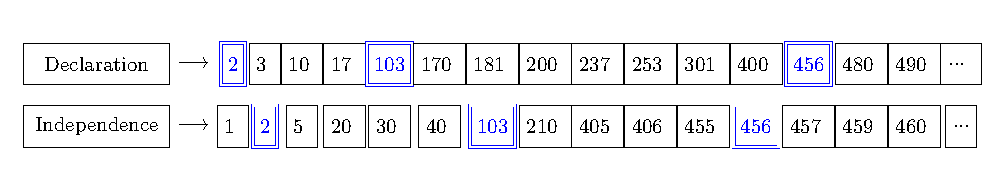
\includegraphics[width=0.7\linewidth,height=\textheight,keepaspectratio,alt={Two postings from the inverted index. Highlighted document IDs with double border indicate matched documents that satisfy Declaration AND Independence.}]{chapters/../assets/figures/chapter12/fig-ir-postings.pdf}

}

\caption{\label{fig-ir-postings}Two postings from the inverted index.
Highlighted document IDs with double border indicate matched documents
that satisfy \emph{Declaration} AND \emph{Independence}.}

\end{figure}%

We now refer to each term's list of documents -- in fact only their IDs
-- as the \emph{posting} of the term. An inverted index is thus a
collection of \emph{postings}. After examining the two postings, we can
conclude that documents \(\#2\), \(\#103\), and \(\#456\) in
Figure~\ref{fig-ir-postings} contain both terms. But how can an
algorithm merge the two postings to identify these matched documents?

A very simple approach is to go through the documents IDs in the posting
for term \emph{Declaration} and, for each of them, we compare it with
every document ID in the second posting for term \emph{Independence}.
Suppose the first posting has \(n_1\) documents and the second has
\(n_2\), this will conduct \(n_1 \cdot n_2\) comparisons. This approach
is going to be very slow with large postings and it has yet to take
advantage of the sorting (pre-computation) that has been performed on
the document IDs.

Apparently, we can improve on the above brute force method is by
conducting a binary search on the second posting for each document on
the first posting. In this case, the time complexity of the matching
process will become \(O(n_1 \log n_2)\) as the binary search is of
\(O(\log n_2)\) complexity. Assume \(n_2 > n_1\) is a large number, this
will significantly reduce query processing time.

So far we have used one posting as the primary to iterate through and,
in the process, compare each value there to those in the second posting.
In this approach, the two postings play unequal roles in the matching
process.

A different approach is to take the postings equally and iterate through
them simultaneously. Assuming document IDs are sorted in the ascending
order, we start at the beginning of each posting. In each step, we
compare the current values of the two postings and the one with a small
value will move to the next (greater) value. This continues until it has
been found a value greater or equal to the current value of the other
posting. In that case, we switch to the other posting to go next.

For the above example, we start at first document ID in each posting
shown in Figure~\ref{fig-ir-matching}, where the \emph{Declaration}
posting has a value \(2\) and the \emph{Independence} posting has \(1\)
(see step 1 in the figure). As the one with a smaller document ID, the
\emph{Independence} posting will move to the next document ID, which is
\(2\) and matches the the current value in \emph{Declaration} (see step
2).

\begin{figure}

\centering{

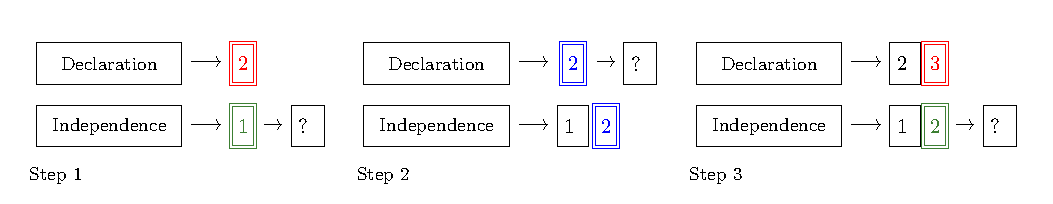
\includegraphics[width=0.7\linewidth,height=\textheight,keepaspectratio,alt={Simultaneous walking to merge postings, starting at the first document ID. The posting with the smaller value will move to the next ID.}]{chapters/../assets/figures/chapter12/fig-ir-matching.pdf}

}

\caption{\label{fig-ir-matching}Simultaneous walking to merge postings,
starting at the first document ID. The posting with the smaller value
will move to the next ID.}

\end{figure}%

Now that the second posting (\emph{Independence}) is already with an
equal or greater document ID, the process will shift to the first
posting (\emph{Declaration}) to catch up, which, as shown in
Figure~\ref{fig-ir-matching} step 3, then goes to document \(\#3\) and
switches the turn back as it surpasses \(2\). This process will continue
until no more matches can possibly be found.

In the worse case scenario, it iterates through the two postings from
start to end, which is \(O(n_1 + n_2)\) time complexity. Practically,
this is better than the previous method with \(O(n_1 \log n_2)\)
complexity where \(\log n_2\) may remain a large number (\(\gg 2\)).

These techniques are particularly useful to merge postings for logical
AND, i.e.~for document containing both or all query terms. They also
work well with the OR query expressions, where documents containing any
of the terms should be brought together after the removal of duplicate
IDs.

The simultaneous iterative process can be further improved with skip
pointers that the iterations faster by skipping a significant amount of
document IDs in each posting. However, the skip pointers technique is of
little use for OR queries as it skips documents that should be included
with a logical OR.

\section{Ranking}\label{ranking}

With techniques presented in the previous section, we know how to
process a query with an inverted index and identify matched documents by
merging postings for the query terms. This can be conducted rather
efficiently if proper preprocessing is already in place, e.g.~with
sorting and skip pointers.

If the user can articulate her need for information with relevant query
terms in a precise boolean expression, then the system should be able to
serve the user's need via matching. There is potentially a long list of
documents that match the query. In the old days, this perhaps worked
just fine for scholars who would like to find a list of research
publications for a comprehensive literature review.

In the context of today's World Wide Web and online social media, it
will not be helpful by retrieving an extremely long list of pages and
presenting them all at once to the user. For one, the query expression
of any ordinary user is most likely imprecise and a lot of matched
documents will turn out to be non-relevant.

More important, many information seekers on the web are not looking for
comprehensive literature. Often they are in need of the one page, if not
a few, that can satisfy their need or at least something they can start
with. In these cases, the challenge is not about the thoroughness of the
result, but how precise and relevant the result is.

The common practice of today's web search engines is to present a ranked
list of matched documents where, ideally, the most relevant documents
will appear early on so the user can see them and follow with a
clickthrough. So in addition to query matching, document ranking
(sorting) in the retrieved result is essential for the success of a
search engine.

\subsection{Content-based Ranking}\label{content-based-ranking}

So in what order shall we rank documents or pages according to a query?
Among the matched ones, what documents should be presented to the user
early in the result?

As the key to \emph{information retrieval} (IR) is relevance, the first
reaction to the questions here is to rank documents according to how
\emph{relevant} they are to the query. But how do we quantify relevance?
Without the user's subjective feedback on what is relevant vs.~what is
not, there is simply no data to quantify relevance. The alternative is
to assume that documents that match the user's query expression to a
higher degree are more relevant to her information need.

Based on this assumption, there are several approaches we can take. For
example, using the \emph{Term Frequency} (TF) scheme discussed in
chapter , we can count the total number of query term occurrences in
each document. The matching score of a document \(d\) with regard to
query \(q\) can be therefore computed by:

\[\begin{aligned}
score(q,d) & = & \sum_{t \in q \cap d} TF_{t,d}
\end{aligned}\]

where \(t\) is each term appearing in both the query and the document,
and \(TF_{t,d}\) is the term frequency of \(t\) in \(d\), i.e.~the
number of times it appears in the document.

Now one would argue that this scoring function will not work well as it
give equal importance to each query term. With this method, one who
issues a query like "the declaration" may retrieve a bunch of documents
with lots of "the" in the writing (suppose "the" has not been removed as
a stop-word from being indexed). We may therefore consider the relevance
of individual terms by replacing the TF with TF-IDF weights (Term
Frequency * Inverse Document Frequency):

\[\begin{aligned}
score(q,d)
% & = & \sum_{t \in q \cap d} w_{t,d} \\
& = & \sum_{t \in q \cap d} TF_{t,d} \cdot IDF_{t}
\end{aligned}\]

where \(IDF_t\) is IDF weight of term \(t\).

Both TF and TF-IDF scoring functions above are dependent on the terms'
occurrences. Apparently, longer documents (e.g.~books) are more likely
to contain more instances of the same terms than the shorter documents.
To remedy for this bias, one can normalize term frequency by the
document length:

\[\begin{aligned}
score(q,d)
& = & \sum_{t \in q \cap d} \frac{TF_{t,d}}{L_d} \cdot IDF_{t}
\end{aligned}\]

where \(L_d\) is the length of document \(d\), i.e.~the number of terms
in the documents including duplicates. Now that we factor in document
length, short documents will have \emph{equal} chances to be ranked and
long documents will no longer dominate\footnote{An alternative to
  document length normalization is to use \emph{cosine similarity}
  instead of a sum of term weights. Cosine is focused on the angle
  proximity (vector direction) in a vector space, which is essentially
  about terms' distributions rather than their absolute occurrences. See
  related discussions in chapter~.}. After all, for any document \(d\),
\(\sum_t \frac{TF_{t,d}}{L_d} = 1\) regardless of its length. This is
after the fact that the overall probability of \emph{any term} drawn
from the document is always \(1\).

The document-length-normalized TF is a a probability estimate. Imagine
if we put all the terms of document \(d\) in a black box and randomly
draw a term from it, the likelihood of getting term \(t\) can be
estimated by \(\frac{TF_{t,d}}{L_d}\). The length-normalized scoring
function here is essentially modeled on the probability of each query
term's occurrence in the document.

Like document-length normalized TF, IDF is also based on a probability
estimate. As discussed in chapter~, a term's IDF weight is also a
measure based on the term's likelihood to appear in any document drawn
randomly from the entire data collection. The component
\(\frac{n_t}{N}\) in the IDF function, where \(N\) is the total number
of documents and \(n_t\) the number of documents containing term \(t\),
is to estimate the term's collection-wide probability. The logarithmic
transformation: \[\begin{aligned}
IDF_t
& = & -\log{\frac{n_t}{N}} \\
& = & \log{\frac{N}{n_t}}
\end{aligned}\]

does convert dramatically varied probability values into a more
comparable scale and dampens their differences. However, this
formulation is not accidental but has in fact a concrete theoretical
root in the information theory. \(IDF_t\) can be derived from measuring
the amount of \emph{relative entropy} (KL divergence) when term \(t\) is
observed in a document from the collection.(Aizawa 2003)

In light of uncertainties involved in understanding user needs to
quantify relevance, one may also think of ranking documents in terms of
the \emph{probability of relevance}. Indeed, early probabilistic IR
research followed the \emph{Probability Ranking Principle} (PRP), which
states that documents should be ranked in order of the probability of
relevance, or how likely documents will be useful to the user.(Robertson
1977) The principle can be operationalized by estimating those
probability from data, e.g.~data on term distributions and user
relevance feedback.

Based on PRP and a logarithmic transformation of the Bayes rule, one can
model the odds of a document's relevance given a query and derive a
weighting function similar to IDF. This is known as the \emph{Binary
Independence Model} (BIM), where the notion of relevance is binary
(either relevant or not relevant)\footnote{This is not to confuse with
  the fact that the probability (of relevance) is still a continuous
  measure, not a binary one. In other words, even though the final
  answer is either yes (1) or no (0), the probability of yes vs.~no
  remains a continuous value between 0 and 1.} and documents are assumed
to be independent of one another (Robertson and Sparck-Jones 1976). The
relevance weight \(w^{RSJ}_t\)\footnote{RSJ stands for Robertson and
  Spark-Jones, the authors of the weighting scheme.} of a term \(t\) in
BIM is computed by:

\[\begin{aligned}
w^{RSJ}_t
& = & \log{\frac{(r_t + 0.5)(N - R - n_t + r_t + 0.5)}{(n_t - r_t + 0.5)(R - r_t + 0.5)}}
\end{aligned}\]

where \(R\) is the number of relevant documents, \(n_t\) is document
frequency of term \(t\), and \(r_t\) is the number of \emph{relevant}
ones in the \(n_t\) documents. The weight approximates IDF when both the
number of relevant documents \(r_t\) is much fewer \(n_t\), which in
turn is much smaller compared to the entire collection \(N\). That is,
\(w^{RSJ}_t \approx IDF_t\) when \(r_t \ll n_t \ll N\).

Further development of this probabilistic model led to another
well-known method called \emph{BM25}(Robertson and Zaragoza 2009), where
a term's weight is computed by:

\[\begin{aligned}
w^{BM25}_{t,d}
& = &
\frac{TF_{t,d}}{k_1(1-b)+b\frac{L_d}{\bar{L}}+TF_{t,d}}
\cdot w^{RSJ}_t
\end{aligned}\]

where \(\bar{L}\) is the average document length in the collection, and
\(k_1\) and \(b\) are parameters to be optimized (tuned) through
experiments. \(b\) adjusts the degree of document normalization, with
full normalization at \(b=1\) and no normalization at \(b=0\). This
highly resembles TF*IDF, where \(w^{RSJ}_t\) corresponds to \(IDF_t\)
and the rest of the formula is \(TF_{t,d}\) with document-length
normalization. The scoring (ranking) function for BM25 is then the sum
of term weights:

\[\begin{aligned}
score(q,d) & = & \sum_{t \in q \cap d} w^{BM25}_{t,d}
\end{aligned}\]

\subsection{Popularity-based Ranking}\label{popularity-based-ranking}

With document ranking methods such as those based on TF*IDF and BM25, an
\emph{information retrieval} system will be able to sort documents
according to their match scores, especially in terms of important
keywords in the user query. This worked well in the traditional library
context, where documents were in fact selected publications such as
books and articles. Because of the editorial processes these
publications went through, the contents of the documents were
trustworthy in general. Ranking based on document content is a sensible
solution in that setting.

When the World Wide Web started to grow in the 1990s, the first
generation of web search engines adopted the same technologies developed
in the libraries and continued to rely on text contents in their
ranking. It soon became clear that this is easily susceptible to
spamming.

The Web is a decentralized space for publication without a central
editorial process. Everyone is a publisher who writes anything he wants,
in his own way of expression. A ranking method based on TF*IDF, for
example, is impacted by TF and IDF. You probably can exert very little
influence on the IDF part as it is a \emph{global} statistic of the
entire web collection. However, if you want to be ranked number one for
queries like "The Declaration of Independence," you simply repeat those
keywords in your page contents.

By simple repetition in the text, you increase the terms' frequencies
(TFs) and therefore the ranking of your page to related queries. The
point here is that page contents on the web are not necessarily
trustworthy and we cannot simply rely on the \emph{claims} of authors in
this rather decentralized, autonomous environment.

Without a central authority that we can trust on individual pages, we
may perhaps consider input from their \emph{peers} -- those who know
these pages and what they have to say about them. On the web, pages
reference one another via \emph{hyperlinks}. Figure~\ref{fig-hlinks}
shows an example of a web page, from which the user can click on a label
(text), a button, or an image to visit another page.

\begin{figure}

\centering{

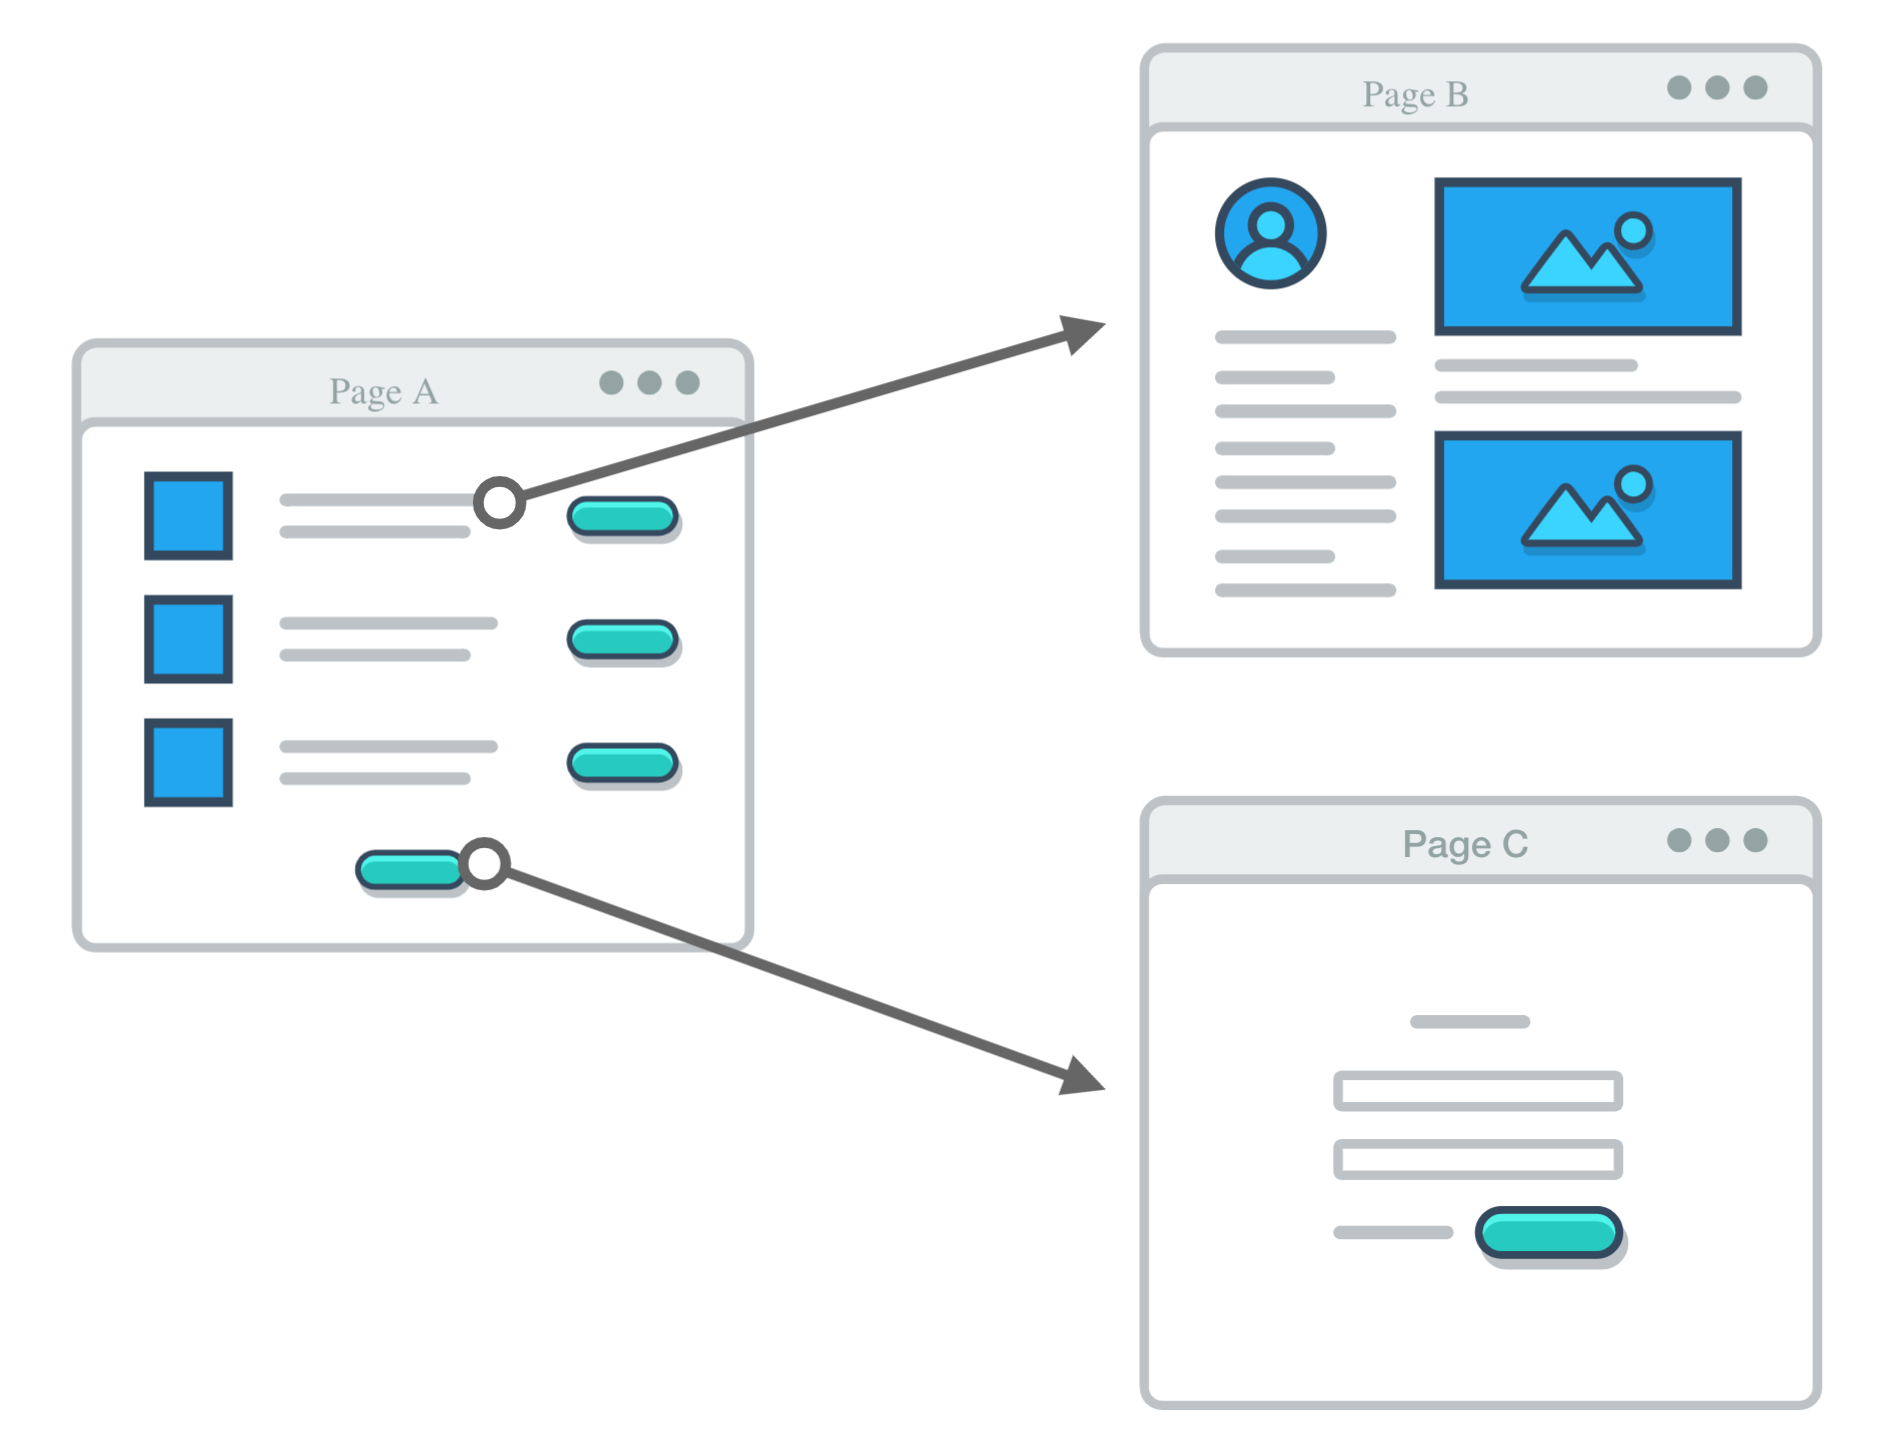
\includegraphics[width=2in,height=\textheight,keepaspectratio,alt={Page references via hyperlinks from page A to pages B and C}]{chapters/../assets/figures/pageflow2.png}

}

\caption{\label{fig-hlinks}Page references via hyperlinks. Page A links
to several other pages, including B and C.}

\end{figure}%

With hyperlinks, we pages form a directed network on which structural
analysis can be performed. And when a text label (i.e.~anchor text) is
provided as part of the hyperlink, it provides useful data about what
the target page is about.

In Figure~\ref{fig-hlinks}, when page A links to page B, descriptions or
keywords page A uses on the hyperlink can be considered for the
representation of page B. Assuming the pages are on different web sites
with separate ownership, then this piece of anchor text represents an
independent evaluation of page B's contents. By aggregating anchor text
data from all other pages linking to page B, its inverted index can be
adjusted with the crowd-sourced data, which are potentially more
reliable than self-claimed page contents.\footnote{Anchor text can also
  be hacked and abused to boost one's search engine ranking. There has
  been known practice of self- or mutual-linking from sites set up by
  the same group of people. On the other hand, websites can team up to
  \emph{bomb} a target with off-topic anchor text in order to "promote"
  its ranking for those keywords, e.g.~for political activism.}

Based on the classic BM25, BM25F is an example of related methods that
go beyond the body text of a web page to include other structural
elements (fields) and relevant data streams (particularly anchor text
data).(Zaragoza et al. 2004) Among others, the use of anchor text data
for indexing and matching is a common practice of web search engines.

When the user issues a search query, the question remains what is more
\emph{relevant} and should be ranked higher in the result. For web
searches, \emph{relevance} does not merely mean \emph{on-topic} because
a very large number of pages will be considered on topic in terms of
their contents (anchor text included). The notion of \emph{relevance}
also entails certain degree of \emph{importance} while on topic.

Importance, however, can be subjective and hard to quantify. To borrow
an idea from \emph{scientometrics}, we can instead substitute
\emph{importance} with \emph{impact} or \emph{popularity}. While in
scholarly communication scientific research is evaluated based on the
amount of citations, web pages can be treated likewise in terms of
hyperlinks.

If we regard each hyperlink as a citation to the target page, we can now
measure a page's impact or popularity by counting the number of incoming
links, i.e.~\emph{in-degree}. That is, the impact score \(R_d\) of a
target document (page) \(d\) is computed by:

\[\begin{aligned}
r_d & = & \sum_{p \in P_d} 1
\end{aligned}\]

where \(P_d\) is the collection of pages linking to \(d\). For each
linking page \(p\), the contribution is considered equal with \(1\). In
Figure~\ref{fig-ir-2links}, for example, page \(t\) has two in-links
from pages \(p_1\) and \(p_2\) and its impact score is therefore \(2\).

\begin{figure}

\centering{

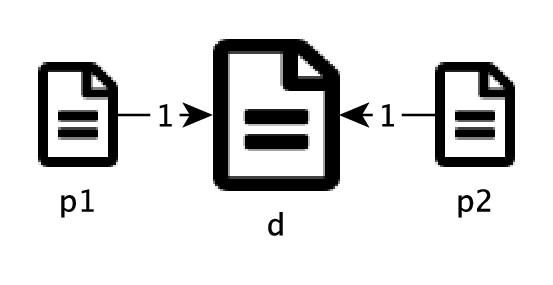
\includegraphics[width=1.5in,height=\textheight,keepaspectratio,alt={Two pages linking to the same target page with equal contributions}]{chapters/../assets/figures/ir/ir_2links.png}

}

\caption{\label{fig-ir-2links}Two links being equal. Without more data,
the two links are assumed to contribute equally to the target page's
impact.}

\end{figure}%

But are all hyperlinks created equal? Let's consider an extreme case
where we have more data for the two linking pages in
Figure~\ref{fig-ir-2links}. Suppose \(p_1\) is an ordinary page that is
linked to by another page but links to many others (including page
\(d\)). On the other hand, \(p_2\) is a very popular page that is
referenced by many pages but has chosen to link to only one page
(i.e.~page \(d\)). Figure~\ref{fig-ir-2links_more} illustrates this
scenario.

\begin{figure}

\centering{

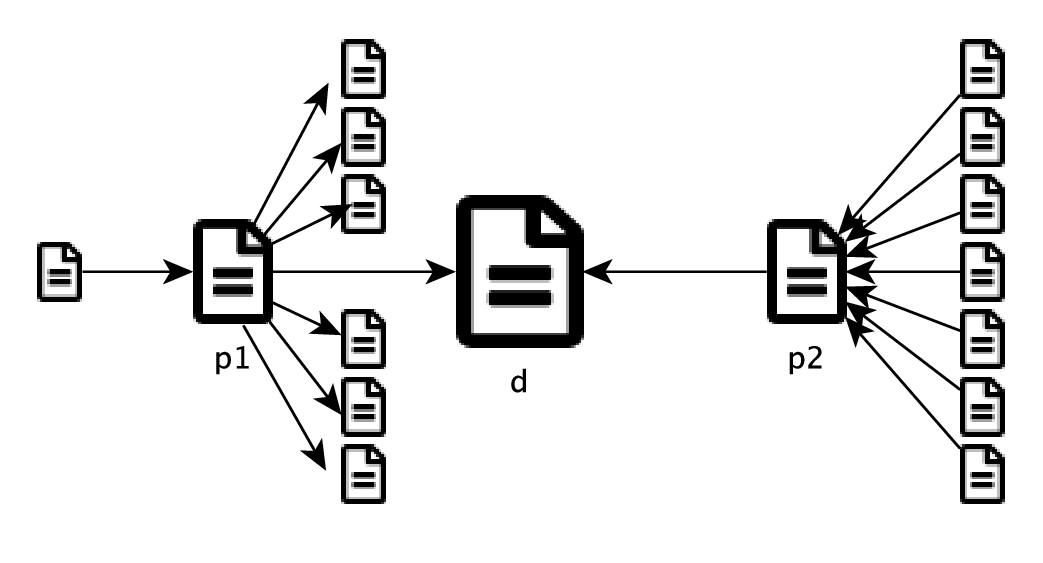
\includegraphics[width=3in,height=\textheight,keepaspectratio]{chapters/../assets/figures/ir/ir_2links_more.png}

}

\caption{\label{fig-ir-2links_more}Two links being different. When we
know more about the pages linking to the target page, we can no longer
assume their contributions are equal.}

\end{figure}%

Based on the above hypothetical scenario, it is apparent that the links
from \(p_1\) and \(p_2\) to the page \(t\) are not equal. For one,
\(p_2\) is much more popular and has more impact than \(p_1\) given the
number of in-links it receives. Moreover, it gives out the only one link
to page \(d\), making its contribution (endorsement) even stronger. On
the contrary, \(p_1\) receives very little (from only one page) and
gives out a lot, further diluting its already small share.

In reality, \(p_2\) can be the page of an influential figure like the
Pope who receives lots of media attention. If he chooses to post only
one link and that goes to your page, you must be thrilled. We can also
think of \(p_1\) as the total opposite, a page of yours or mine with a
long list of notes and references. The longer the list goes, the less
significant each reference may become.

This discussion sheds lights on two important aspects for scoring a
page's impact or popularity. First, it matters who gives the link and
how impactful the \emph{link giver} is. A link from an important figure
should carry more weight in itself. Second, it also matters how many
links the giver \emph{gives out}. When one gives out to more recipients,
the share of each link is diluted and the weight should be divided by
the number of out-links. Mathematically, the second aspect can be easily
quantified by counting the out-links for each page in \(P\).

On the first point, however, the solution does not appear
straightforward. Again in Figure~\ref{fig-ir-2links_more}, the impact of
document \(d\) depends on the impact of linking pages \(p_1\) and
\(p_2\), which in turn depend on the ones that link to them. And this
will go on. How can we proceed to solve this problem of \emph{chicken
and egg} without going into a loop? But the solution is indeed a loop,
or a recursive process.

\subsection{PageRank}\label{pagerank}

The \emph{directed graph} of web pages pointing to one another can be
thought of as a city of one-way streets (hyperlinks) you can follow and
locations (pages) that you can visit via these streets. If you want to
simply explore the city, you can randomly pick a street to get where it
leads to. Then from there, you can pick a random street again and
continue on.

Imagine if you continue this over and over again, ultimately you may be
able to reach every corner of the city (if every location is connected).
Over time, you will be able to visit some locations for many times. And
chances are, you will visit some locations more often than others -- in
other words, some locations are more \emph{popular} than others on your
tireless, random tour of the city.

So which ones will be visited more frequently by chance? Apparently,
those with more incoming streets, which in turn have more incoming
streets, and so on. And this appears to match the problem we had
earlier, where we wanted to calculate the impact or popularity score of
a page, which depends on the impact of linking pages, which in turn
depends on their linking pages, and so on.

In this thinking, the impact or popularity score of a web document
(similar to a location in the above imaginary city) is equivalent to its
\emph{chance} (frequency) of being visited on a random walk over time --
that is, its \emph{long-term visit rate}.

This is essentially the \emph{Random Surfer} (random "walker" on the
web) model proposed for the Google's original \emph{PageRank}\footnote{While
  PageRank is indeed about ranking \emph{pages} on the web, the name is
  in fact after its primary author and Google co-founder, Larry Page.}
function.(Page et al. 1999) In this model, the computer simulates a user
following the link structure of the web after pages have been collected
(crawled) and parsed. It starts at any page and, at each step, goes out
along one (randomly chosen) of the links on page to reach another.
Ultimately, each page will have a long-term visit rate if this
simulation is conducted with sufficient time (to reach the steady
state).

There is one problem, however. Some pages do not have out-links -- they
are dead ends where the surfer will get stuck. To avoid this issue, the
surfer should be allowed to jump (\emph{teleport}) out of the current
page to visit another random page. Also for pages with few or no
in-links to be visited a bit more frequently -- so that they are no
totally disregarded in the ranking model -- the surfer will
\emph{teleport} periodically regardless of out-links. The probability
associated with this periodic teleporting is referred to as the
\emph{damping factor}. With this model, the impact score \(r_d\) of a
page \(d\) is equivalent to the long-term visit rate, which is computed
by:

\[\begin{aligned}
r_d & = & \alpha \sum_{p \in P_d} \frac{r_p}{n_p} + \beta
\end{aligned}\]

where \(n_p\) is the out-degree (number of out-links) of page \(p\),
which links to \(d\) and is having a current score of \(r_p\). On the
right side of the equation, the first part \(\alpha \sum r_p /n_p\) is
the score one receives from in-links and the term \(\beta\) represents
the amount each page is given "for free." Both \(\alpha\) and \(\beta\)
can be regarded as parameters related to the damping factor.

For example, with a periodic teleporting probability of \(0.15\), we can
set \(\alpha = 1 - 0.15 = 0.85\) for the earned portion (from links) and
\(\beta = 0.15 \frac{1}{N}\) for the "free" portion, where \(N\) is the
total number of documents (pages) in the collection.\footnote{The
  original PageRank paper used \(0.15\) for the damping factor based on
  earlier experimental results.} In this way, \(\beta\) represents the
chance each page will be visited with teleporting.

With equation~\hyperref[eq-pagerank]{{[}eq-pagerank{]}}, one needs to
follow the recursive approach of a random surfer to calculate the
ultimate PageRank scores for all pages. Because we do not know these
values (i.e.~the \(r_p\) values), which are needed to start the
computation (i.e.~to calculate \(r_d\)), we will kick off with arbitrary
initial values, for example, by setting every page's score to \(1/N\) --
that is, they are treated equally likely to be visited before we proceed
to find out the actual values. In each iteration, we update the all
pages' scores using equation~\hyperref[eq-pagerank]{{[}eq-pagerank{]}}
until there is very little or no change at all to the scores.

In the end, the PageRank score of a page corresponds to the probability
that the page will be visited by the random surfer. The more prominent a
page is in the web graph, the more likely (frequently) it will be
visited and therefore will have a higher PageRank score. PageRank scores
are query independent as they are only determined by the network
structure. When a search engine ranks pages with regard to a specific
user query, results should first limited to those meeting query criteria
before PageRanks are combined with query-related weights such as those
based on TF*IDF.

Although the basic version of PageRank computes its scores regardless of
a query, one can easily modify
equation~\hyperref[eq-pagerank]{{[}eq-pagerank{]}} to make it
query-dependent. For example, the \(\beta\) does not have to be a
universal constant for all the pages. If we assume each document (page)
can have its individual \(\beta_d\) value, then the PageRank function
becomes:

\[\begin{aligned}
r_d & = & \alpha \sum_{p \in P_d} \frac{r_p}{n_p} + \beta_d
\end{aligned}\]

where we may assign different \(\beta_d\) to pages based on, for
example, other indicators about their relevance to a search query.

PageRank, which is essentially a \emph{centrality} measure in network
analysis, is an extension of computing eigenvector and Katz
centrality.(Newman 2010) The Hyperlink-Induced Topic Search algorithm,
or HITs, can be regarded as a further extension of PageRank.(Kleinberg
1999) While PageRank only considers contributions from in-links, HITS
gives credit to pages that point to others (out-links) as well. With
\emph{hub} (centrality based on out-links) and \emph{authority}
(centrality based on in-links), the algorithm propagates the scores in a
similar iterative process until stabilized.

With HITS, the analysis is performed on a sub-collection including pages
relevant to a query (text-wise) as well as other pages with in-links
from and/or out-links to the relevant ones. This setup makes HITS
query-dependent and the relevance to a query is reinforced through the
propagation of \emph{hubs} and \emph{authorities}.

\section{Information Filtering}\label{information-filtering}

\emph{Information Filtering} (IF) looks at the same information seeking
problem from the opposite angle of IR -- instead of reaching out to find
information, IF is to eliminate the non-relevant so that the user only
receives the relevant. IR and IF are considered to be "two sides of the
same coin."(Belkin and Croft 1992)

\emph{Information filtering} usually operates on an ongoing information
stream such as emails. Look at how many junk emails or spams\footnote{We
  refer to relevant emails as \emph{hams} and the irrelevant as
  \emph{spams}.} you receive daily and you see the importance of having
a good spam filter. Filtering for recommendation, e.g.~on news and
movies, is another popular application of information filtering.

One major challenge in information filtering is the information stream
that constantly feeds and changes in its content. Patterns that you have
discovered from past spam emails, for example, may turn out to be
useless for future spam filtering as spammers learn and change their
behavior. News that you used to follow closely may become irrelevant in
the next news cycle or as your interests move on. It requires constant
learning of the user and the environment to adapt to the ongoing
changes.

\section{Questions}\label{questions}

I do want to stress the key advantage AND disadvantage of normalization,
which is to treat terms of different forms as the same.

1) There are situations in which the different variations are indeed
about the same and should be treated as one term. This way, users who
uses one variation in the query may be able to find documents containing
terms in another.

2) But there are also situations where normalization is an
over-treatment and can lead to results that are in fact not relevant
(false positives). There are plenty of examples in both 1) and 2). In
specific domains, there might be more in 1) vs.~2), or vise versa. By
examining your domain data and use cases, you may find whether it is
better to do certain normalization or not (e.g.~casefolding, but not
stemming).

Now, we have increasingly more storage and computing power at a cheaper
price. So often we can do more with these technologies. For example, it
is common to have multiple indices even for the same data, e.g.~one with
certain normalization and one without. Then at search time, you combine
evidence from all indices to final matching and ranking of results.

We know terms have different discriminative powers -- that some terms
are more useful than the others. We know stopwords (highly frequent
terms) are generally less useful. What about rare terms, i.e., terms
that are used in a very tiny portion of documents? What about terms in
between (neither rare or too frequent)? If you have to choose a limited
number of terms to index your documents, what kind of terms would you
pick?

In the vector space model, cosine similarity is often used to measure
how close (or distant) two vectors are? For example, you can compare a
query (vector) with each document (vector), and rank them according to
their cosine similarities. Given that cosine is about the angle (vector
directions) and disregards vector magnitude (length), why is vector
direction more important than magnitude here (for term-based text
representation)?

Your analogue is good in that both "generators" are in a dynamic process
of generating something, which can trap a crawler in their space (in
both worlds).

The generator here in the context of the web is a general reference to
dynamic web pages that generate page contents based on different given
parameters.

An example of this is the "next page" link to help users navigate to
additional lists of information. An ordinary user may click on "next",
and "next", ... for a few iterations.

But a spider, without sufficient intelligence and design, may go on and
on by simply "clicking" on (following) the "next page" link nonstop...
The notion of "trap" goes both ways -- it traps the crawler on the site
gathering data on and on; but it also leads to intensive load on the
generator (as there appear to be lots of clicks and page loads to the
web server). Years ago when I was a graduate student, I developed a
crawler with an aim to collect all web pages of the entire university
(where I was studying) and, the first night I ran it, it was able to
collect 2 million+ pages with a cost. The crawler was trapped by another
college/school's site with a page "generator" and, in the end, brought
the entire server down... You can imagine what happened the next morning
when the IT manager found out... And it did take me some time to settle
the issue as as a student. ;)

Good question.

For website or pages that no one knows and links to, crawlers won't be
able to collect them. A crawler starts with seed websites (those already
known) and, ultimately, will get to those where there is a path. But
there are "islands" to which there is no path. There are also pages that
can be reached from certain parts of the web and cannot be reached
either unless you have seeds to crawl from specific locations...

There is always a part of the web where crawlers cannot penetrate. We
generally refer to this as the deep web. There are private sites, sites
with access control, and sites that can be interacted with but too
difficult for crawler to collect... they represent a space much much
greater than the regular web covered by search engines. 

\section*{Exercise}\label{exercise}
\addcontentsline{toc}{section}{Exercise}

\markright{Exercise}

Assume we have a tiny collection of two documents with the following
terms: Doc 1: apple, pear, dessert, cream, cook, work, berry Doc 2:
work, computer, disk, apple, network, system Given a free text query
"apple computer," rank the documents using Dice's coefficient. Please
provide the formula and list calculation steps.

Which ones (more than one) of the following statements about Euclidean
distance are true? It measures that distance between the end points of
two vectors. It measures that angle between two vectors. Euclidean
distance is affected by vector magnitudes. Euclidean distance is zero
when two vectors point to the same direction.

Which ones (more than one) of the following statements about Cosine
similarity are true? It measures that distance between the end points of
two vectors. It measures that angle between two vectors. Cosine is
affected by vector magnitudes. Cosine is 1 (max value) when two vectors
point to the same direction.

Does vector length normalization (dividing a vector by its
length/magnitude) have any impact on Cosine ranking?

\chapter{Graphs and Structural Analysis}\label{ch-graphs}

\section{Graphs as Data}\label{graphs-as-data}

\section{Paths, Connectivity, and
Traversal}\label{paths-connectivity-and-traversal}

\section{Centrality and Influence}\label{centrality-and-influence}

\section{Communities and Structural
Roles}\label{communities-and-structural-roles}

\section{Link Prediction}\label{link-prediction}

\section{From Graph Features to Graph
Learning}\label{from-graph-features-to-graph-learning}

\section{Summary, Exercises, and Lab}\label{summary-exercises-and-lab-2}

\part{Trustworthy and Practical Machine Learning}

\chapter{Evaluation and Experimentation}\label{ch-evaluation}

Imagine you are asked to design an algorithm to help detect credit card
fraud. Suppose you are told that your algorithm will be tested for its
accuracy and, as a way to motivate you, your boss promises a bonus based
on its accuracy. Accuracy, as it turns out, can be roughly defined as
the fraction of answers that are correct. In the context of credit card
fraud detection, one can produce a confusion matrix by cross-examining
predictions (model) vs.~real outcomes (ground truth):

\protect\phantomsection\label{tab-eval-cmatrix}
\begin{longtable}[]{@{}lcc@{}}
\caption{A confusion matrix}\tabularnewline
\toprule\noalign{}
& Predicted Positive \(\hat{\oplus}\) & Predicted Negative
\(\hat{\ominus}\) \\
\midrule\noalign{}
\endfirsthead
\toprule\noalign{}
& Predicted Positive \(\hat{\oplus}\) & Predicted Negative
\(\hat{\ominus}\) \\
\midrule\noalign{}
\endhead
\bottomrule\noalign{}
\endlastfoot
Actual Positive \(\oplus\) & True Positive (TP) & False Negative (FN) \\
Actual Negative \(\ominus\) & False Positive (FP) & True Negative
(TN) \\
\end{longtable}

Based on the counts in Table~\hyperref[tab-eval-cmatrix]{1.1}, accuracy
can be computed by:

\[\begin{aligned}
  Accuracy & = & \frac{TP + TN}{TP + TN + FP + FN}
\end{aligned}\]

which is again the total number of correct answers (true positive and
true negative) divided by the total number of answers.

Given the evaluation based on accuracy, how would you do to maximize
your reward? Surely you can develop a very sophisticated algorithm with
massive data and effort. There is, nonetheless, a simple response to
this challenge. If you look at statistics on credit cards, fraud
transactions represent only a very small fraction. Suppose the
likelihood of a fraud is \(10\) out of every \(1000\). One may simply
classify all \(1000\) transactions as non-fraud and the confusion matrix
will become:

\protect\phantomsection\label{tab-eval-cmatrix0}
\begin{longtable}[]{@{}lcc@{}}
\caption{Confusion matrix based on the zero-effort solution, by
classifying all transactions to non-fraud.}\tabularnewline
\toprule\noalign{}
& Predicted Fraud & Predicted Non-Fraud \\
\midrule\noalign{}
\endfirsthead
\toprule\noalign{}
& Predicted Fraud & Predicted Non-Fraud \\
\midrule\noalign{}
\endhead
\bottomrule\noalign{}
\endlastfoot
Actual Fraud & 0 & 10 \\
Actual Non-Fraud & 0 & 990 \\
\end{longtable}

And the accuracy is:

\[\begin{aligned}
  Accuracy
  & = & \frac{0 + 990}{1000} \\
  & = & 0.99
\end{aligned}\]

This solution requires virtually zero effort but its accuracy appears to
be pretty good: \(99\%\). There are several reasons why an overall
accuracy can be rather misleading, if not completely useless here. For
one, the evaluation metric ignores the data distribution among class
labels (e.g.~fraud vs.~non-fraud) and does not account for potential
\emph{chance} accuracy. In the above example, it is very easy to cheat
and get rewarded just \emph{by chance}. Here you simply favor the
dominant class (non-fraud) to boost accuracy.

Second, an evaluation metric should align properly with the purpose of
the assigned task. For credit card fraud detection, one can argue that
missing a \emph{fraud} transaction is much more costly and undesirable
than misclassifying a normal transaction as fraud. In other words, one
should be motivated to identify most if not \emph{all} fraud
transactions; and the result should be heavily penalized if real frauds
are identified as non-fraud (false negative). We shall look into these
issues to see what alternatives may offer.

\section{Precision}\label{precision}

Given a skewed distribution of data in the classes, it may be useful to
evaluate accuracy within each predicted class. This is equivalent to a
metric commonly known as \emph{precision}, which is the fraction of
those predicted positive to a class that actually belong to that class.
In terms of the confusion matrix Table~\hyperref[tab-eval-cmatrix]{1.1},
precision is computed by:

\[\begin{aligned}
  Precision
  & = & \frac{TP}{TP + FP}
\end{aligned}\]

When both \(TP\) and \(FP\) are zero, precision is \(1\) (\(100\%\)) by
definition. Based on the numbers in
Table~\hyperref[tab-eval-cmatrix0]{1.2}, we can compute precision for
those predicted to be fraud (in the first column of numbers):

\[\begin{aligned}
  Precision(fraud)
  & = & \frac{0}{0 + 0} \\
  & = & 1
\end{aligned}\]

This does not seem to resolve the issue with accuracy, to which
precision is very similar. This is due to the second reason we
discussed, that there should be a greater emphasis and penalty on the
\emph{false negative}. Now instead of looking at the columns to compute
precision, we can examine the rows and evaluate the same result from a
very different perspective.

\section{Recall}\label{recall}

\emph{Recall}, a classic evaluation metric, refers to the fraction of
actual positive that have been classified positive. In the example here,
it is the fraction of real fraud transactions that have been identified
as such. Recall can be computed in terms of the confusion matrix
Table~\hyperref[tab-eval-cmatrix]{1.1}:

\[\begin{aligned}
  Recall
  & = & \frac{TP}{TP + FN}
\end{aligned}\]

where false negative (FN) is part of the denominator. Applying this to
data in Table~\hyperref[tab-eval-cmatrix0]{1.2}, we get a recall of:

\[\begin{aligned}
  Recall(fraud)
  & = & \frac{0}{0 + 10} \\
  & = & 0
\end{aligned}\]

By focusing on true positive vs.~false negative, recall gives a better
indication than precision on the poor performance in fraud detection.
Precision and recall are often used together in evaluation. It is
attempting to compute an average score of the two so there is only one
score to represent the overall performance. The arithmetic mean of
precision and recall here is \((1+0)/2 = 0.5\), which still appears too
good for a zero-effort solution.

Arithmetic mean gives equal weights to both metrics and is not very
indicative of the overall performance. We suggest that such an
"averaging" measure show an alarming score if one of the scores is
extremely low -- that is, we will regard a method as bad if it performs
miserably in one metric. One function that leans more heavily on the
lower score is the \(F\) measure of precision and recall:

\[\begin{aligned}
  F_\beta
  & = & (1+\beta^2) \frac{Precision \cdot Recall}{\beta^2 \cdot Precision + Recall}
\end{aligned}\]

where \(\beta\) value can be adjusted in favor of precision or recall.
When \(\beta=1\), this becomes the \(F_1\) measure, i.e.~the
\emph{harmonic mean}:

\[\begin{aligned}
  F_1
  & = & \frac{2 \cdot Precision \cdot Recall}{Precision + Recall}
\end{aligned}\]

With \(Precision=1\) and \(Recall=0\) in the above example, the harmonic
mean is \(F_1=0\) -- here, the one zero score (recall in this case)
completely dominates and the average suffers.

In applications where a model can be adjusted or tuned, we can evaluate
the model based on more than one pairs of precision and recall scores. A
common practice is to plot the precision-recall curve.
Figure~\ref{fig-eval-pr_curve} shows precision-recall curves of two
methods, where method 1 appears to perform better as its curve is closer
to the top-right (higher precision and recall).

\begin{figure}

\centering{

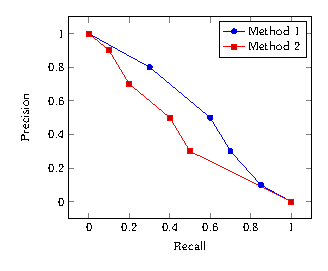
\includegraphics[width=0.7\linewidth,height=\textheight,keepaspectratio,alt={Precision-recall curve}]{chapters/../assets/figures/chapter14/fig-eval-pr-curve.pdf}

}

\caption{\label{fig-eval-pr_curve}Precision-recall curve}

\end{figure}%

\section{Sensitivity and Specificity}\label{sensitivity-and-specificity}

Precision and recall are both focused on the fraction of true positive.
Recall is also referred to as the \emph{true positive rate} (TPR),
sensitivity, or the probability of detection. It measures how
\emph{sensitive} a method is in identifying the actual positives.

Conversely, one can also measure the \emph{true negative rate} (TNR) or
the fraction of actual negatives that have been correctly identified as
such. This is often referred to as \emph{specificity}, which is computed
by:

\[\begin{aligned}
  Specificity
  & = & \frac{TN}{TN + FP}
\end{aligned}\]

Sensitivity and specificity are concepts relative to the class in
question. Sensitivity for the \emph{fraud} class is specificity for the
\emph{non-fraud} class; and vise versa.

The false negative rate (FNR) is complementary to specificity or the
true negative rate (TNR), i.e.~\(FNR=1 - TNR\), and is often referred to
as fall-out or \emph{probability of false alarm}. Similar to precision
vs. recall, sensitivity and fall-out (i.e.~1 - specificity) are often
plotted to produce an \emph{ROC}\footnote{ROC stands for \emph{receiver
  operating characteristic} and was initially used in the military to
  evaluate the performance of a radar detector.} curve.

ROC analysis has been widely used and well studied for model performance
assessment in many fields including defense and medicine. It not only
enables the evaluation of model effectiveness in terms of true positive
and true negative rates, but can also help identify best practice with
cost constraints.

\begin{figure}

\centering{

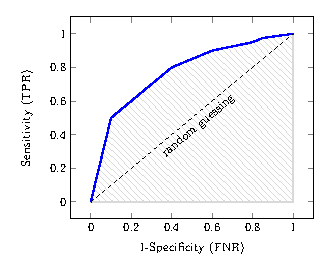
\includegraphics[width=0.7\linewidth,height=\textheight,keepaspectratio,alt={ROC curve and area under curve (AUC)}]{chapters/../assets/figures/chapter14/fig-eval-roc.pdf}

}

\caption{\label{fig-eval-roc}ROC curve and area under curve (AUC)}

\end{figure}%

Figure~\ref{fig-eval-roc} illustrates a plot of an ROC curve, where the
diagonal line (dashed) defines the acceptable performance. To understand
what the diagonal line means, imagine we create a random model that
takes a 50-50 guess during classification. As a result of this random
guessing, there will be an equal split between the predicted positives
\(\hat{\oplus}\) and predicted negatives \(\hat{\ominus}\). Hence,
column values of the same row in Table~\hyperref[tab-eval-cmatrix]{1.1}
will be identical:

\[\begin{aligned}
  N_{\hat{\oplus}} & = & N_{\hat{\ominus}} \\
  TP & = & FN \\
  FP & = & TN
\end{aligned}\]

where \(N_{\hat{\oplus}}\) and \(N_{\hat{\ominus}}\) are the numbers of
predicted positives and negatives respectively. It follows that
\(TPR = FNR\), i.e.~\(Sensitivity = 1 - Specificity\) or
\(Sensitivity + Specificity=1\). This equation defines the diagonal line
in Figure~\ref{fig-eval-roc} and is the result of random guessing.

Below the diagonal line \(Sensitivity+Specificity=1\), the model
performs worse than random and is undesirable. The farther the ROC curve
is above the diagonal line, the better the performance with a greater
area under curve. Therefore, the \emph{area under curve} (AUC), i.e.~the
shaded area in the plot, is a single score that can be computed to
measure the overall performance in terms of ROC.

\section{Kappa and Chance Agreement}\label{kappa-and-chance-agreement}

So far the metrics are focused on different aspects of the confusion
matrix in evaluation. However, we are yet to address one important
problem in assessing the agreement between the predicted and the ground
truth -- chance agreement. A method may hit the correct answer simply by
chance. The evaluation cannot be fairly conducted unless we find a way
to discount the chance agreement.

Let's first look at some of the chances or probabilities. In binary
classification, for example, the outcome is either positive (e.g.~fraud)
or negative (e.g.~non-fraud). Based on the confusion matrix
Table~\hyperref[tab-eval-cmatrix]{1.1}, the likelihood of a positive
prediction vs.~a negative prediction can be estimated:

\[\begin{aligned}
  P(\hat{\oplus})
  & = & \frac{N_{\hat{ \oplus}}}{N} \\
  & = & \frac{TP + FP}{TP + FN + FP + TN} \\
  P(\hat{\ominus})
  & = & \frac{N_{\hat{\ominus}}}{N} \\
  & = & \frac{TN + FN}{TP + FN + FP + TN}
\end{aligned}\]

where \(N_{\hat{\oplus}}\) and \(N_{\hat{\ominus}}\) are the number of
predicted positive and negative answers respectively. \(N\) is the total
number of instances. \(TP+FP\) is the sum of the \emph{Predicted
Positive \(\hat{\oplus}\)} column where as \(TN+FN\) is the sum of the
\emph{Predicted Negative \(\hat{\ominus}\)} column in
Table~\hyperref[tab-eval-cmatrix]{1.1}. These are probabilities of model
predictions.

Likewise, we can estimate probabilities of having a positive vs.
negative outcome in the ground truth:

\[\begin{aligned}
  P(\oplus)
  & = & \frac{N_{\oplus}}{N} \\
  & = & \frac{TP + FN}{TP + FN + FP + TN} \\
  P(\ominus)
  & = & \frac{N_{\ominus}}{N}  \\
  & = & \frac{TN + FP}{TP + FN + FP + TN}
\end{aligned}\]

where \(N_{\oplus}\) and \(N_{\ominus}\) are the numbers of actual
positive and negative results respectively. \(TP+FN\) is the sum of the
\emph{Actual Positive} row and \(TN+FP\) is the sum of the \emph{Actual
Negative} row in Table~\hyperref[tab-eval-cmatrix]{1.1}. These are
probabilities based on the ground truth.

With these probability, it is now possible to estimate chance agreement.
If we assume the model and ground truth are independent, then the
(hypothetical) probabilities that they will reach the same conclusion,
namely the joint probability of both saying "yes" (positive) and the
joint probability of both saying "no" (negative) can be computed by:

\[\begin{aligned}
  P_e(\oplus \cap \hat{\oplus}) & = & P(\oplus) P(\hat{\oplus}) \\
  P_e(\ominus \cap \hat{\ominus}) & = & P(\ominus) P(\hat{\ominus})
\end{aligned}\]

The overall chance agreement, the probability of either both "yes" or
both "no" is:

\[\begin{aligned}
   P_e
   & = & P_e[ (\oplus \cap \hat{\oplus}) \cup  (\ominus \cap \hat{\ominus})]  \\
   & = & P_e(\oplus \cap \hat{\oplus}) + P_e(\oplus \cap \hat{\oplus})  \\
   & = & P(\oplus) P(\hat{\oplus}) + P(\ominus) P(\hat{\ominus})
\end{aligned}\]

Note that we add the two probabilities to compute the OR (\(\cup\))
probability because \emph{positive} and \emph{negative} are mutually
exclusive.

Now that we know the chance agreement \(P_e\), we can use it to discount
the overall agreement \(P_o\):

\[\begin{aligned}
   \kappa & = & \frac{P_o - P_e}{1 - P_e}
\end{aligned}\]

where \(P_o\) is the relative agreement of two, e.g.~two raters such as
a model and an expert (the ground truth), and is identical to the
accuracy metric in our discussion \(P_o = Accuracy\). This is commonly
known as the \emph{Kappa} coefficient, a statistic that measures the
agreement of two sets of results.

As Equation~\hyperref[eq-eval-kappa]{{[}eq-eval-kappa{]}} shows, Kappa
takes into account potential agreement by chance and discounts the
overall coefficient by the chance agreement. This makes it harder for a
model to "cheat" on the result by simply favoring the dominant classes
(e.g.~classifying all transactions into non-fraud).

With the result in Table~\hyperref[tab-eval-cmatrix0]{1.2}, the chance
agreement \(P_e\) is:

\[\begin{aligned}
  P_e
  & = & P(\oplus) P(\hat{\oplus}) + P(\ominus) P(\hat{\ominus}) \\
  & = & \frac{10}{1000} \times 0 + \frac{990}{1000} \times \frac{1000}{1000} \\
  & = & 0.99
\end{aligned}\]

By discounting this chance agreement, we get a \emph{Kappa} coefficient
of zero:

\[\begin{aligned}
  \kappa
  & = & \frac{P_o - P_e}{1 - P_e} \\
  & = & \frac{0.99 - 0.99}{1 - 0.99} \\
  & = & 0
\end{aligned}\]

A kappa score of \(0\) does not mean there is no agreement. There is in
fact an agreement between the model prediction and the ground truth.
However, this agreement is purely due to chance and is reduced to \(0\)
after discounted for the chance agreement.

Indeed, \(\kappa=0\) means completely chance agreement. Its minimum
value, \(\kappa=-1\), indicates total disagreement whereas a maximum
value \(\kappa=1\) shows the two are in full agreement even after
accounting for chances.

\section{Averaging}\label{averaging}

When evaluating model performance on multiple classes -- even binary
classification entails two classes -- there are two major strategies to
compute an overall score (average).

Suppose precision is the evaluation metric, one can construct a
confusion matrix for each class \(c\) and compute its precision by:

\[\begin{aligned}
  P_c & = & \frac{TP_c}{TP_c + FP_c}
\end{aligned}\]

And the overall (average) precision can be computed by:

\[\begin{aligned}
  \bar{P}_{macro} & = & \frac{\sum_{c \in C} P_c}{|C|}
\end{aligned}\]

where \(C\) is the set of unique classes and \(|C|\) is the size of the
set or the number of classes, e.g.~\(2\) for binary classification. This
is \emph{macro averaging}, which computes the average based on
class-level scores. It gives equal treatment to each class and disregard
their relative sizes (significance).

The alternative is micro averaging which takes into account the
composition of each classes and produces a final average weighted by
class sizes. With micro averaging, all related counts are summed up
before a ratio is taken. For example, average precision can be computed
by:

\[\begin{aligned}
  \bar{P}_{micro} & = & \frac{\sum_{c \in C} TP_c}{\sum_{c \in C} TP_c + FP_c}
\end{aligned}\]

This turns out to be the overall fraction of predictions that are
correct -- in fact, a micro averaged precision is identical to
\emph{accuracy} in binary classification.

Whether one should use macro or micro averaging depends on the relative
importance of classes in the final assessment. If all classes are
equally important regardless of their sizes, macro-averaging should be
preferred. If one aims to emphasize the absolute number of correct
predictions, then micro-averaging is appropriate.

\section{Rank Evaluation}\label{rank-evaluation}

There are applications where the focus is not about definitive correct
vs.~incorrect answer. In information retrieval, for example, a model may
return a sorted list of search results. Such a rank list requires a
different approach to evaluation.

Surely one can regard a rank list as the set of correct answers and use
the discussed metrics such as precision and recall. More precisely, we
can create a cut-off at a certain position \(k\) in the rank and use the
top \(k\) as the set to be evaluated. For example, precision at \(k=10\)
is useful to evaluate early results in web searches, where the emphasis
is often on the first result page (top \(10\)).

If one knows the total number of relevant document \(r\) (recall) for a
query, the cut-off can be set at position \(r\) to measure it precision.
This is referred to as \emph{R-Precision} because at this particular
position precision is equal to recall. It is also possible to measure
average precision by starting with the top position \(k=1\) and
increasing it until recall reaches \(100\%\).

Several other metrics can be derived from variations of these
strategies. However, they only attack the problem of rank list
evaluation by indirectly addressing positions in the list.

A direct attack on this issue is to assign a \emph{different score}
(amount of reward) for a correct (relevant) answer in a \emph{different
position}. A relevant answer at the top should be highly rewarded, which
should be discounted down the rank.

This is the idea behind the \emph{Normalized Discounted Cumulative
Gain}, or nDCG, which has been widely used in the information retrieval
community since its proposal.(Järvelin and Kekäläinen 2002) Given the
relevance \(rel_i\)\footnote{Relevance scores can be on any scale
  dictated by the evaluation protocol. For example, they can be as
  simple as \(1\) for a relevant (correct) answer and \(0\) if
  otherwise.} of an answer at position \(i\), the Discounted Cumulative
Gain at position \(k\) can be computed by:

\[\begin{aligned}
  DCG_k
  & = & \sum_{i=1}^{k} \frac{rel_i}{\log_2(i+1)} \\
  & = & rel_i + \sum_{i=2}^{k} \frac{rel_i}{\log_2(i+1)}
\end{aligned}\]

where a relevant (correct) answer at position \(1\) will receive its
full credit and others will be discounted by their positions down the
rank, with \(\log_2(i+1)\).

Among all possible arrangements of the rank list for a query, there
exists at least one ideal (perfect) list in which answers are sorted by
their relative relevance scores in the descending order. This produces
the best possible DCG score, which we call the ideal DCG or IDCG.
Comparing a DCG score against its corresponding ideal score, we can
obtain the \emph{normalized} DCG or nDCG:

\[\begin{aligned}
  nDCG_p & = & \frac{DCG_p}{IDCG_p}
\end{aligned}\]

Normalized by the ideal score, an nDCG score is always between
\([0, 1]\), with \(1\) indicating a perfect ranking and \(0\) no
relevant answer at all in the list\footnote{Here assume relevance scores
  are non-negative, e.g.~\(0\) no reward for non-relevance. In certain
  applications, it might be reasonable to assign negative scores for
  non-relevant answers to penalize a ranking with any non-relevant
  results.}. nDCG is a popular metric for web search evaluation and one
can adjust the position \(k\) to emphasize relevant results at the very
top, e.g.~with \(nDCG_3\).

\section{Evaluation of Numeric
Predictions}\label{evaluation-of-numeric-predictions}

When the outcome of a model is a on a continuous scale rather than
discrete values, the evaluation is no longer about \emph{correct}
answers because it is rarely possible to make predictions that are
\emph{exactly} the actual outcome. Instead, the focus should be on how
closely predictions are to the actual values or how much apart they are
(errors).

\subsection{Error Metrics}\label{error-metrics}

Many evaluation metrics for numeric predictions are indeed based on the
error terms. The mean absolute error (MAE), mean squared error (MSE),
and root mean-squared error (RMSE), for example, compute mean errors in
their absolute, squared, and root squared forms:

\[\begin{aligned}
  MAE & = & \frac{\sum_{i=1}^{N} |\hat{v}_i - v_i|}{N} \\
  MSE & = & \frac{\sum_{i=1}^{N} (\hat{v}_i - v_i)^2}{N} \\
  RMSE & = & \sqrt{\frac{\sum_{i=1}^{N} (\hat{v}_i - v_i)^2}{N}}
\end{aligned}\]

where \(N\) is the total number of instances to test the numeric
predictions, \(\hat{v}_i\) is the predicted value on the \(i^{th}\)
instance, and \(v_i\) is the actual value of the \(i^{th}\) instance.
Relatively speaking, metrics based on squared errors such as MSE and
RMSE are amplify the impact of large errors and are more sensitive to
outliers.

Each of these error metrics can be normalized by the corresponding error
of a pseudo-model predicting the mean value of training data, to obtain
its \emph{relative} error. For example, relative squared error (RSE) can
be computed by:

\[\begin{aligned}
RSE & = & \frac{\sum_{i=1}^{N} (\hat{v}_i - v_i)^2}{\sum_{i=1}^{N} (\bar{\mu} - v_i)^2}
\end{aligned}\]

where \(\bar{\mu}\) is the estimated mean based on training data. Root
relative squared error (RRSE) and relative absolute error (RAE) can be
established in the like manner.

\subsection{Correlation}\label{correlation}

While RSE measures the deviation of predicted values \(\hat{v_i}\) from
actual values \(v_i\), standard deviations of predicted and actual
values can be computed by:

\[\begin{aligned}
  \sigma & = & \sqrt{\frac{\sum_{i=1}^{N} (v_i - \mu)^2}{N-1}} \\
  \hat{\sigma} & = & \sqrt{\frac{\sum_{i=1}^{N} (\hat{v}_i - \hat{\mu})^2}{N-1}}
\end{aligned}\]

where \(\mu\) is the mean of actual values and \(\hat{\mu}\) the mean of
predicted values. The covariance between the predicted and actual is:

\[\begin{aligned}
  cov(\hat{v},v) & = & \frac{\sum_{i=1}^{N} (\hat{v}_i - \hat{\mu})(v_i - \mu)}{N-1}
\end{aligned}\]

By normalizing the covariance by the product of both standard deviations
(also a value of variance), we can obtain the Pearson correlation
between the predicted and actual values:

\[\begin{aligned}
  cor(\hat{v},v)
  & = & \frac{cov(\hat{v},v)}{\hat{\sigma}\sigma} \\
  & = & \frac{\sum_{i=1}^{N} (\hat{v}_i - \hat{\mu})(v_i - \mu)}{\sqrt{\sum_{i=1}^{N} (v_i - \mu)^2} \sqrt{\sum_{i=1}^{N} (\hat{v}_i - \hat{\mu})^2}}
\end{aligned}\]

Pearson correlation measures the similarity in their variances from
means and is equivalent to cosine of \(v\) and \(\hat{v}\) as vectors
from their means. Figure~\ref{fig-eval-cor} illustrates the connection
using a 2-dimensional space. To simplify the discussion, suppose there
are only \(N=2\) instances on which the actual outcomes are
\((v_1, v_2)\) and predicted values are \((\hat{v_1},\hat{v_2})\), with
means \(\mu\) and \(\hat{\mu}\) respectively.

\begin{figure}

\centering{

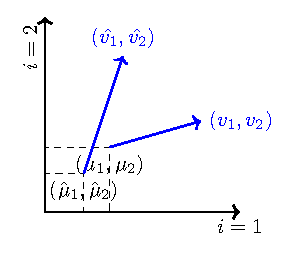
\includegraphics[width=0.7\linewidth,height=\textheight,keepaspectratio,alt={Pearson correlation as cosine of vectors originated from means, with N=2 for a 2-dimensional visualization}]{chapters/../assets/figures/chapter14/fig-eval-cor.pdf}

}

\caption{\label{fig-eval-cor}Pearson correlation as cosine of vectors
originated from means, with \(N=2\) for a 2-dimensional visualization}

\end{figure}%

As shown in Figure~\ref{fig-eval-cor}, the actual values can be regarded
as a vector pointing in the \(\vec{v} = (v_1-\mu, v_2-\mu)\) direction,
whereas the predicted is represented by the vector
\(\vec{\hat{v}}=(\hat{v_1}-\hat{\mu}, \hat{v_2}-\hat{\mu})\). In this
representation, Pearson correlation is identical to the cosine of the
two vectors, i.e.~\(cov(\hat{v}, v) = cosine(\vec{\hat{v}},\vec{v})\).
Chapter~ has more on the cosine similarity.

Because of this connection, Pearson correlation shares important
characteristics with cosine. It reaches its maximum value of \(1\) when
errors from their mean, i.e.~\(\hat{v_i} - \hat{\mu}\) vs.~\(v_i - \mu\)
for all instances, are distributed identically (in the same vector
direction) -- they are perfectly correlated in this case. When the
errors are distributed in absolutely \emph{orthogonal} directions, the
two are perfectly independent and has no correlation. When their errors
distribute in the opposite direction, they are negatively correlated,
with the minimum value of \(-1\) indicating perfectly opposite.

\section{Experimentation}\label{experimentation}

Now that we know some of the metrics for model evaluation, how do we
actually conduct the assessment with data? In the ideal world, one
builds a model using training data with known outcomes and rolls out the
model to be tested in the operating environment. In the real world,
however, we have to make sure a model works reliably well for its
purpose before it is used in production for important predictions and
decision making.

We often have to use existing data to test models with experiments. It
is a common practice to split the data into training and testing subsets
-- one to build and train the model, and the other to evaluate its
performance.

Random sampling can be used to create the training and testing subsets.
Once a model is trained, it can be experimented with the test data and
evaluated using metrics suitable for related objectives. This process
can be repeated to test different models or the same model with
different parameters or configurations. It can be done with different
random samples.

Along the process, one may be able to find out what leads to best
performances in terms of certain metrics. Given various model
configurations, it is also possible to create plots such as
precision-recall or ROC curves, where one can examine related parameters
and tradeoffs.

The ratio to split training vs.~testing depends the amount of available
data and the amount required to sufficiently train the specific model.
One may be tempted to conduct a 50-50 split. In this case, you use half
of the data (sample) for training and the other half for testing.
Afterwards, it also makes sense to switch the two subsets, testing data
now for training and training for testing.

This is cross validation. And you can do it on 50-50, a 2-fold
validation, you can certainly do it on more folds. Practically, it is
popular to conduct a 10-fold cross validation, where the data is split
into 10 random subsets. Each time, \(1\) subset is held out for testing
and the other \(9\) are used for training. This is repeated \(10\) times
so the model is tested on every fold of the data.

\section{On Efficiency}\label{on-efficiency}

In this chapter, we have focused on the evaluation of model
\emph{effectiveness} or, loosely speaking, how satisfactory predictions
are compared to the ground truth. This is about the \emph{quality} of a
model.

The other side of evaluation is on the \emph{efficiency} of operations.
This is about the time and cost necessary to train a model and to
perform assigned tasks. It depends on the space and time complexity of
the model, and the structure and magnitude of data the model has to work
on in the production settings.

A thorough evaluation should include an assessment of both effectiveness
and efficiency. We will elaborate on important aspects of efficiency as
well as \emph{scalability} in Chapter .

\chapter{Generalization, Model Selection, and
Fit}\label{ch-generalization}

Torture the data, and it will confess to anything.

\emph{Ronald Coase}

\section{Training Performance and
Generalization}\label{training-performance-and-generalization}

\section{Bias, Variance, and Model
Capacity}\label{bias-variance-and-model-capacity}

\section{Validation and
Cross-Validation}\label{validation-and-cross-validation}

\section{Regularization}\label{regularization-1}

\section{Learning Curves and
Diagnostics}\label{learning-curves-and-diagnostics}

\section{Hyperparameter Selection Without
Leakage}\label{hyperparameter-selection-without-leakage}

\section{Summary, Exercises, and Lab}\label{summary-exercises-and-lab-3}

Under- and over-fitting...

Bias, variance, and error...

Combined, ensemble learning...

\chapter{Scaling, Deployment, and Responsible Use}\label{ch-scaling}

\section{Time, Space, Data, and
Compute}\label{time-space-data-and-compute}

\section{Batch, Streaming, and Distributed
Workflows}\label{batch-streaming-and-distributed-workflows}

\section{From Experiment to Reproducible
Pipeline}\label{from-experiment-to-reproducible-pipeline}

\section{Deployment, Monitoring, and
Drift}\label{deployment-monitoring-and-drift}

\section{Privacy, Security, and
Misuse}\label{privacy-security-and-misuse}

\section{Energy, Sustainability, and
Proportionality}\label{energy-sustainability-and-proportionality}

\section{Responsible Decisions and Human
Oversight}\label{responsible-decisions-and-human-oversight}

\section{Summary and Exercises}\label{summary-and-exercises-1}

\bookmarksetup{startatroot}

\chapter*{References}\label{references}
\addcontentsline{toc}{chapter}{References}

\markboth{References}{References}

\protect\phantomsection\label{refs}
\begin{CSLReferences}{1}{1}
\bibitem[\citeproctext]{ref-Aizawa2003IDF}
Aizawa, Akiko. 2003. {``An Information-Theoretic Perspective of TF-Idf
Measures.''} \emph{Information Processing and Management} (Tarrytown,
NY, USA) 39 (1): 45--65.
\url{https://doi.org/10.1016/S0306-4573(02)00021-3}.

\bibitem[\citeproctext]{ref-Barabasi1999}
Barabási, Albert-László, and Réka Albert. 1999. {``Emergence of Scaling
in Random Networks.''} \emph{Science} 286 (5439): 509--12.
\url{https://doi.org/10.1126/science.286.5439.509}.

\bibitem[\citeproctext]{ref-Bekenstein:2003}
Bekenstein, Jacob D. 2003. {``Information in the HOLOGRAPHIC
UNIVERSE.''} \emph{Scientific American} 289 (2): 58--65.
\url{http://www.jstor.org/stable/26060403}.

\bibitem[\citeproctext]{ref-Belkin1992IF}
Belkin, Nicholas J., and W. Bruce Croft. 1992. {``Information Filtering
and Information Retrieval: Two Sides of the Same Coin?''} \emph{Commun.
ACM} (New York, NY, USA) 35 (12): 29--38.
\url{https://doi.org/10.1145/138859.138861}.

\bibitem[\citeproctext]{ref-Cover:1967}
Cover, T., and P. Hart. 1967. {``Nearest Neighbor Pattern
Classification.''} \emph{IEEE Transactions on Information Theory} 13
(1): 21--27. \url{https://doi.org/10.1109/TIT.1967.1053964}.

\bibitem[\citeproctext]{ref-Endres:2006}
Endres, D. M., and J. E. Schindelin. 2006. {``A New Metric for
Probability Distributions.''} \emph{IEEE Transactions on Information
Theory} (Piscataway, NJ, USA) 49 (7): 1858--60.
\url{https://doi.org/10.1109/TIT.2003.813506}.

\bibitem[\citeproctext]{ref-Jarvelin:2002}
Järvelin, Kalervo, and Jaana Kekäläinen. 2002. {``Cumulated Gain-Based
Evaluation of IR Techniques.''} \emph{ACM Trans. Inf. Syst.} (New York,
NY, USA) 20 (4): 422--46. \url{https://doi.org/10.1145/582415.582418}.

\bibitem[\citeproctext]{ref-Kaggle:2017}
Kaggle. n.d. \emph{The State of Data Science \& Machine Learning 2017}.
\href{https://www.kaggle.com/surveys/2017}{Https://www.kaggle.com/surveys/2017}.

\bibitem[\citeproctext]{ref-Ke:2015}
Ke, Weimao. 2015. {``Information-Theoretic Term Weighting Schemes for
Document Clustering and Classification.''} \emph{International Journal
on Digital Libraries} 16 (2): 145--59.
\url{https://doi.org/10.1007/s00799-014-0121-3}.

\bibitem[\citeproctext]{ref-Ke:2017}
Ke, Weimao. 2017. {``Text Retrieval Based on Least Information
Measurement.''} \emph{Proceedings of the ACM SIGIR International
Conference on Theory of Information Retrieval} (New York, NY, USA),
ICTIR '17, 125--32. \url{https://doi.org/10.1145/3121050.3121075}.

\bibitem[\citeproctext]{ref-Kleinberg1999HITS}
Kleinberg, Jon M. 1999. {``Authoritative Sources in a Hyperlinked
Environment.''} \emph{J. ACM} (New York, NY, USA) 46 (5): 604--32.
\url{https://doi.org/10.1145/324133.324140}.

\bibitem[\citeproctext]{ref-Kullback:1951}
Kullback, S., and R. A. Leibler. 1951. {``On Information and
Sufficiency.''} \emph{Annals of Mathematical Statistics} 22: 79--86.
\url{https://doi.org/10.1214/aoms/1177729694}.

\bibitem[\citeproctext]{ref-Manning2008IIR}
Manning, Christopher D., Prabhakar Raghavan, and Hinrich Schütze. 2008.
\emph{Introduction to Information Retrieval}. Cambridge University
Press.

\bibitem[\citeproctext]{ref-Mooers1951IR}
Mooers, Calvin N. 1951. {``Zatocoding Applied to Mechanical Organization
of Knowledge.''} \emph{American Documentation} 2 (1): 20--32.
\url{https://doi.org/10.1002/asi.5090020107}.

\bibitem[\citeproctext]{ref-Newman2010Networks}
Newman, Mark. 2010. \emph{Networks: An Introduction}. Oxford University
Press, Inc.

\bibitem[\citeproctext]{ref-PageRank99}
Page, Lawrence, Sergey Brin, Rajeev Motwani, and Terry Winograd. 1999.
\emph{The PageRank Citation Ranking: Bringing Order to the Web.}
Technical Report Nos. 1999-66. Stanford InfoLab; Stanford InfoLab.
\url{http://ilpubs.stanford.edu:8090/422/}.

\bibitem[\citeproctext]{ref-Price1976}
Price, Derek De Solla. 1976. {``A General Theory of Bibliometric and
Other Cumulative Advantage Processes.''} \emph{Journal of the American
Society for Information Science} 27 (5): 292--306.
\url{https://doi.org/10.1002/asi.4630270505}.

\bibitem[\citeproctext]{ref-Rapoport:1953}
RAPOPORT, ANATOL. 1953. {``WHAT IS INFORMATION?''} \emph{ETC: A Review
of General Semantics} 10 (4): 247--60.
\url{http://www.jstor.org/stable/42581363}.

\bibitem[\citeproctext]{ref-Robertson1977PRP}
Robertson, Stephen. 1977. {``The Probability Ranking Principle in
{IR}.''} \emph{Journal of Documentation} 33 (December): 294--304.
\url{https://doi.org/10.1108/eb026647}.

\bibitem[\citeproctext]{ref-Robertson1976BIM}
Robertson, Stephen, and Karen Sparck-Jones. 1976. {``Relevance Weighting
of Search Terms.''} \emph{Journal of the American Society for
Information Science} 27 (May): 129--46.
\url{https://doi.org/10.1002/asi.4630270302}.

\bibitem[\citeproctext]{ref-Robertson2009PRF}
Robertson, Stephen, and Hugo Zaragoza. 2009. {``The Probabilistic
Relevance Framework: BM25 and Beyond.''} \emph{Foundations and Trends in
Information Retrieval} (Hanover, MA, USA) 3 (4): 333--89.
\url{https://doi.org/10.1561/1500000019}.

\bibitem[\citeproctext]{ref-Shannon1948}
Shannon, Claude E. 1948. {``A Mathematical Theory of Communication.''}
\emph{Bell System Technical Journal} 27: 379-423 and 623-656.

\bibitem[\citeproctext]{ref-Yang:1997}
Yang, Yiming, and Jan O. Pedersen. 1997. {``A Comparative Study on
Feature Selection in Text Categorization.''} \emph{Proceedings of the
Fourteenth International Conference on Machine Learning} (San Francisco,
CA, USA), ICML '97, 412--20.
\url{http://dl.acm.org/citation.cfm?id=645526.657137}.

\bibitem[\citeproctext]{ref-Zaragoza2004BM25F}
Zaragoza, H., N. Craswell, M. Taylor, S. Saria, and S. E. Robertson.
2004. {``Microsoft Cambridge at TREC 2004: Web and HARD Track.''}
\emph{The Thirteenth Text Retrieval Conference (TREC 2004)}, 1--7.

\bibitem[\citeproctext]{ref-Zipf:1949}
Zipf, George K. 1949. \emph{Human Behaviour and the Principle of Least
Effort}. Addison-Wesley.

\end{CSLReferences}


\backmatter


\end{document}
